\chapter{Results}
\label{chap: Results}

\todo{add chapter introduction}

\section{Experimental Setup and Conventions}
\label{sect: 4_setup}

Every hybrid run reported in this chapter is accompanied by a reference simulation $\mathcal{S}_\text{ref}$ that is advanced purely by WaterLily. The reference simulation is instantiated using the exact same initial condition of the hybrid simulation $u_0$ at $t^*=0$. This initial condition is a saved flow state taken from a previously developed simulation, so the wake has already reached the fully developed, periodic vortex-shedding regime, and the trajectories are free of transient start-up effects. This means that $\mathcal{S}$ and $\mathcal{S}_\text{ref}$ are exact copies of each other in terms of grid, immersed geometry and time-stepping parameters, and are integrated with the same solver during each conventional CFD step. The reference simulation is never re-synchronised to the hybrid state: once the two share an initial condition, they evolve as two independent trajectories, with $\mathcal{S}_\text{ref}$ representing the outcome the conventional solver would have produced if there weren't any latent-space acceleration. This allows us to quantify the effects of the pipeline integrations, since the two simulations differ only in whether the latent dynamics $f_\phi$ are used to advance the simulation.

All runs reported in this chapter use the serial execution mode, explained in \autoref{subsect: serial_exec}: the data-collection, training, hybrid-loop and retraining phases execute sequentially within a single allocation, so each phase's wall time adds directly to the total. The parallel model of \autoref{subsect: parallel_exec} is the intended deployment but is not implemented here and left as a setup for future work; the speed-up metrics below (\autoref{subsect: 4_metrics}) are defined on this additive, non-overlapping basis.

The simulation clocks are kept aligned by monitoring the mismatch in $t^*$ across the simulations. After each update of $\mathcal{S}$, be it a numerical CFD step or a latent rollout, $\mathcal{S}_\text{ref}$ is advanced by repeated solver steps, governed by the CFL condition \cite{Weymouth2025}, until its convective time $t^*(\mathcal{S}_\text{ref})$ has caught up to that of the hybrid simulation, so the two are co-located in $t^*$ to within a single time step at every checkpoint.

While both simulations advance in time, relevant mean flow components (time-averaged velocity, pressure, and velocity fluctuations) are stored in the WaterLily \texttt{MeanFlow} object. The mean flow components of the hybrid and reference simulations are sampled at fixed intervals. It is important to note that during the latent rollout (\autoref{alg: predict_flex}), each new latent vector $\tilde{\mathbf{z}}$ that corresponds to the saving interval for the mean flow components is also saved, batched and decoded together with the final rollout prediction that has not been flagged as OOD by the KNN monitor, this assures that the mean flow components of the hybrid simulation are updated using the exact same amount of snapshots at the same $t^*$. 



\subsection{Comparison metrics} 
\label{subsect: 4_metrics}
Because the cylinder wake at $Re = 2500$ is chaotic, the hybrid and reference trajectories can quickly separate in time when given a slight perturbation in the velocity field. Because of this, comparing $\mathcal{S}$ and $\mathcal{S}_\text{ref}$ using a pointwise field error is not a meaningful measure of accuracy, and is therefore not used. The simulations are instead compared through statistical and integral quantities, which are the physically reproducible observables of the flow.

\subsubsection{Computational cost}
The primary motivation of the hybrid scheme is acceleration, so the first metric to compare is wall time. Both simulations integrate the identical convective-time window $0 \mapsto t^*_\text{end}$ on the same hardware, so the ratios below isolate the algorithmic gain rather than a platform difference. Two speed-up metrics are reported:

\begin{align}
  S_\text{loop} = \frac{T_\text{wall}^\text{ref}}{T_\text{wall}^\text{h, cfd} + T_\text{wall}^\text{h, rollout}} = \frac{T_\text{wall}^\text{ref}}{T_\text{wall}^\text{h, tot}},
  \qquad
  S_\text{eff}
  = \frac{T_\text{wall}^\text{ref}}{T_\text{wall}^\text{h, tot} + T_\text{wall}^\text{h, training}}
\end{align}
Where $S_\text{loop}$ is the speedup achieved by the hybrid loop (\autoref{alg: run_hybrid}); the denominator splits the loop costs into conventional CFD steps that stabilise the field between rollouts, $T_\text{wall}^\text{h, cfd}$, and the latent rollouts of $\mathcal{P}$, $T_\text{wall}^\text{h, rollout}$. It reflects the cost of hybrid ML-CFD timestepping after the ML models have been trained. $S_\text{eff}$ additionally charges the training costs $T_\text{wall}^\text{h, training}$ of the networks in $\mathcal{P}$, and is able to quantify the speed-up of the complete integrated workflow of \autoref{fig: workflow_serial}. 

\subsubsection{Integrated forces}

Pressure force coefficients are used to compare performance in an engineering context. It allows the verification of the hybrid loop using the integrated loading on the cylinder, independent of where in the wake the two solutions agree. The
time-mean drag $\langle C_D \rangle$ and the root-mean-square lift $C_L^\text{rms}$ are compared against the reference, as shown in
\autoref{fig: 256_forces}, through their absolute errors

\begin{align}
  e_{C_D} &= \bigl| \langle C_D \rangle - \langle C_D \rangle_\text{ref} \bigr|,
  &
  e_{C_L} &= \bigl| C_L^\text{rms} - C_{L,\text{ref}}^\text{rms} \bigr|,
\end{align}
together with their relative counterparts 
\begin{align}
  e^\text{rel}_{C_D} &= \frac{\bigl| \langle C_D \rangle - \langle C_D \rangle_\text{ref} \bigr|}{C_{D, \text{ref}}},
  &
  e^\text{rel}_{C_L} &= \frac{\bigl| C_L^\text{rms} - C_{L,\text{ref}}^\text{rms} \bigr|}{C_{L,\text{ref}}^\text{rms}},
\end{align}

The mean drag coefficient allows the assessment of the physically meaningful streamwise loading, whereas the mean lift coefficient vanishes due to symmetry, so the fluctuation amplitude $C_L^\text{rms}$ is compared. The comparison of the relative errors allows comparison between different hybrid simulations. These integral force metrics confirm loading but tell nothing about the errors in the wake of the simulation, which motivates the comparison metrics of the field quantities below. 

\subsubsection{Mean flow and Reynolds stresses}
 Each time-averaged field is compared against its reference cell-by-cell over the fluid domain $\Omega$ through two complementary metrics, namely the mean absolute error (MAE):
 
\begin{align}
\varepsilon_q
  = \frac{1}{N_\Omega}\sum_{\mathbf{x}\in\Omega}
    \bigl\lvert q(\mathbf{x}) - q_\text{ref}(\mathbf{x}) \bigr\rvert,
\qquad
q \in \bigl\{ \langle u\rangle,\, \langle v\rangle,\,
              \langle u'u'\rangle,\, \langle v'v'\rangle,\,
              \langle u'v'\rangle \bigr\},
\end{align}
      
with $N_\Omega$ the number of fluid cells, which quantifies the pointwise error in magnitude between $\mathcal{S}$ and $\mathcal{S}_\text{ref}$. The spatial Pearson correlation coefficient measures whether the two fields share the same spatial structure independent of amplitude:
\begin{align}
\rho_q
  = \frac{\sum_{\mathbf{x}\in\Omega}
           \bigl(q - \bar{q}\bigr)
           \bigl(q_\text{ref} - \bar{q}_\text{ref}\bigr)}
         {\sqrt{\sum_{\mathbf{x}\in\Omega}\bigl(q - \bar{q}\bigr)^2}\;
          \sqrt{\sum_{\mathbf{x}\in\Omega}
                \bigl(q_\text{ref} - \bar{q}_\text{ref}\bigr)^2}},
\qquad
\bar{q} = \frac{1}{N_\Omega}\sum_{\mathbf{x}\in\Omega} q(\mathbf{x}),
\end{align}
     
The two are complementary: $\varepsilon_q$ captures the amplitude bias of $\mathcal{P}$ directly, whereas $\rho_q$ stays near unity as long as the wake topology is preserved, even when the fluctuation magnitudes are damped.


All of the metrics above are expressed over the full simulation time window (unless mentioned otherwise), being $0 \mapsto t^*_\text{end}$, which includes all CFD sections in the initial data-gathering, hybrid, training and retraining phases of the acceleration workflow. 

\subsection{Execution environment and hardware mapping}
\label{subsect: 4_hardware}

All reported hybrid simulations were carried out on a single \texttt{gpu-a100} node of the DelftBlue HPC cluster~\cite{DHPC2024}; the node hardware and the requested SLURM allocation are summarised in \autoref{tab: hardware}. A single job requested 12 of the node's 64 CPU cores and one of its four A100 GPUs; the remaining cores and GPUs are unused.

\begin{table}[htbp]
  \centering
  \begin{tabular}{lll}
    \toprule
              & \texttt{gpu-a100} node                              & Requested per run \\
    \midrule
    CPU       & 2$\times$ Intel Xeon Gold 6448Y, 64 cores @ 2.1\,GHz & 12 cores          \\
    GPU       & 4$\times$ NVIDIA A100 80\,GB                         & 1$\times$ A100 80\,GB \\
    Memory    & 512\,GB                                             & 48\,GB            \\
    \bottomrule
  \end{tabular}
   \caption{DelftBlue \texttt{gpu-a100} node hardware and the per-run SLURM allocation used throughout this chapter.}
  \label{tab: hardware}
\end{table}

However, not all phases highlighted in \autoref{fig: workflow_serial} are run on the same device. Only the autoencoder training $(\varphi_\theta,\psi_\theta)$ is placed on the A100: because this training procedure is dominated by dense, batched convolutions over the $256\times256$ velocity fields, all of which are operations that efficiently map onto the GPU architecture. Every other component ($\mathcal{S}_\text{ref}$, initial data-collection, retraining data-collection, stabilisation CFD steps, the neural ODE training $f_\phi$, and the latent rollout) runs on the 12 CPU cores. Both $\mathcal{S}$ and $\mathcal{S}_\text{ref}$ are advanced on WaterLily's multithreaded-CPU backend, with Julia launched on the 12 available threads so that the solver's kernel loops get parallelised across the 12 allocated cores.

This split in devices is deliberate. The neural ODE is a small network whose training and inference costs are dominated by the sequential ODE solve and reverse-mode differentiation; as a result, neither its training nor its inference benefits from running on GPU hardware in this case, so placing $f_\phi$ on the A100 would yield little performance benefit. Furthermore, the CFD domain being relatively small at $256^2$ ($\sim$0.07\,M DOF) also means that it does not benefit from the advantages of WaterLily's GPU backend, since that advantage only materialises once the GPU memory is substantially filled~\cite{Weymouth2025}. With neither phase able to use the GPU optimally, mapping them onto the GPU means repeatedly transferring small arrays across the CPU--GPU boundary to feed kernel operations that are too cheap to recoup the transfer overhead. Because the transfer cost outweighs any benefit the GPU could provide in these phases, every component except autoencoder training is run on the CPU. Keeping all timed phases on the same device also has a methodological advantage: the reported $S_\text{loop}$ becomes a CPU-to-CPU comparison on identical hardware, isolating the algorithmic gain of the hybrid loop rather than conflating it with differences between devices.


\section{Hybrid Acceleration of the Cylinder Flow}
\label{sect: 4_base_hybrid}

\subsection{Baseline Configuration}
\label{subsect: 4_baseline}
As a starting point for presenting the acceleration results, a base pipeline $\mathcal{P}$ is set up against which all subsequent experiments are compared. The hyperparameters for each $\mathcal{P}$ component ($\varphi_\theta, \; \psi_\theta, \; f_\phi, \; \mathcal{K}$) are listed and discussed in the paragraphs below.

\subsubsection{Autoencoder}
Following the autoencoder design choices highlighted in \autoref{sect: AE}, a baseline autoencoder is constructed. The autoencoder is to minimise the physics-informed loss function \autoref{eq: AE_loss}, using the $L_1$ reconstruction term with the divergence and curl regularisers. The baseline architecture was chosen via a grid search tuning. That swept over latent dimensions $N_Z$, physics informed weights $\lambda_\text{div},\,\lambda_\text{curl}$, convolutional blocks $n_\text{conv}$ and dense bottleneck layers $n_\text{dense}$. The exact scoring mechanism and all other evaluated models are discussed in \autoref{app: ae_arch}. 

\begin{table}[H]
    \centering
    
    \begin{tabular}{@{}llc@{}}
        \toprule
        Hyperparameter & Symbol & Value \\
        \midrule
        \multicolumn{3}{l}{\textit{Architecture}} \\
        Latent dimension          & $N_z$            & $16$ \\
        % Input channels            & $C_\text{in}$    & $4$  \\
        % Output channels           & $N_u$            & $2$  \\
        Convolutional blocks      & $n_\text{conv}$  & $5$  \\ % TODO confirm: code default = 5
        Dense bottleneck layers   & $n_\text{dense}$ & $1$  \\ % TODO confirm: code default = 1
        Base channel count        & $C_\text{base}$  & $8$  \\
        Convolution kernel        & $k$              & $3$  \\
        Pooling kernel            & $p$              & $2$  \\
        Convolution stride        & $s$              & $1$  \\
        \midrule
        \multicolumn{3}{l}{\textit{Training}} \\
        Reconstruction loss       & --                      & $L_1$ \\
        Divergence weight         & $\lambda_\text{div}$    & $100$ \\ % TODO confirm: slides = 1000
        Curl weight               & $\lambda_\text{curl}$   & $100$ \\
        Weight decay              & $\lambda$               & $9\times10^{-4}$ \\
        Learning rate             & $\eta$                  & $1\times10^{-3}$ \\
        Retrain Learning rate     & $\eta_r$                & $2\times10^{-4}$ \\
        Optimiser                 & --                      & AdamW \\ % TODO confirm AE optimiser
        Batch size                & --                      & $16$  \\
        Epochs                    & --                      & $500$ \\
        Retrain Epochs            & --                      & $100$ \\
        Trajectory Downsample     & --                      & $300$ \\
        Train - Validation split  & --                      & $0.2$ \\
        Initial Test split        & --                      & $0.25$ \\
        \bottomrule
    \end{tabular}
    \caption{Baseline autoencoder configuration.}
    \label{tab: 4_ae_config}
\end{table}

An interesting thing to note is the choice of $n_\text{dense}$. During hyperparameter optimisation, the resulting score in \autoref{tab: ae_grid_sweep} consistently favoured a single dense bottleneck layer ($n_\text{dense}=1$) over deeper alternatives. This reduces the dense stack in the encoder to a linear compression from the last feature map $H_{n_\text{conv}}\!\cdot\! W_{n_\text{conv}}\!\cdot\! C_{n_\text{conv}}$ to the latent space, meaning the encoder gains nothing from the additional ReLU nonlinearity in the intermediate dense layers for this compression case. The reason is that the additional ReLU activations rectify the negative values of the latent dynamics to zero, as shown in \autoref{fig: activations}. These negatively signed latent dynamics are essentially lost and cannot be recovered by the encoder. This loss of latent information directly degrades reconstruction quality, which is why deeper dense stacks score worse in the sweep.


The choice for $n_\text{conv}$ shows that convolution up to a small spatial dimension (like in the example architecture in \autoref{fig: encoder}) is also adversarial to autoencoder performance, showing how a feature map with small spatial dimensions can not contain enough information to accurately be compressed to a latent vector $\mathbf{z}$. Which is why the autoencoder tuning scheme preferred five $n_\text{conv}$ to the deeper options

% \todo{come back to this}

\subsubsection{Neural ODE}
\label{subsubsect: 4_baseline_node}

The latent dynamics $\frac{\partial{\mathbf{z}}}{\partial t} = f_\phi(\mathbf{z})$ are parametrised by a single-hidden-layer multilayer perceptron and trained with the multiple-shooting loss~\eqref{eq: node_loss_ms}. The hidden width is set by $\texttt{dense\_mult}\times N_z$, and the shooting hyperparameters correspond to the group size $n_s$ and continuity weight $\lambda_c$ as introduced in \autoref{subsect: NODEtraining}. 

\begin{table}[H]
    \centering
    \begin{tabular}{@{}llc@{}}
        \toprule
        Hyperparameter & Symbol & Value \\
        \midrule
        \multicolumn{3}{l}{\textit{Network}} \\
        Latent dimension          & $N_z$                & $16$ \\
        Hidden-width multiplier   & \texttt{dense\_mult} & $2$  \\ % TODO confirm: slides = 3
        Hidden layers             & --                   & $1$  \\
        Activation                & --                   & \texttt{tanhshrink} \\
        \midrule
        \multicolumn{3}{l}{\textit{Integration}} \\
        ODE solver                & --                   & \texttt{Tsit5} \\
        Relative tolerance        & --                   & $1\times10^{-3}$ \\
        Absolute tolerance        & --                   & $1\times10^{-5}$ \\
        \midrule
        \multicolumn{3}{l}{\textit{Training}} \\
        Optimiser                 & --                   & AdamW \\
        Learning rate             & $\eta$               & $1\times10^{-2}$ \\
        Iterations                & --                   & $300$ \\
        Retrain Iterations        & --                   & $150$ \\
        Group size                & $n_s$                & $15$  \\
        Continuity weight         & $\lambda_c$          & $200$ \\
        Retrain Continuity Weight & $\lambda_{c, r}$     & $400$ \\
        Training samples          & --                   & $300$ \\
        \bottomrule
    \end{tabular}
    \caption{Baseline neural ODE configuration.}
    \label{tab: 4_node_config}
\end{table}

As discussed in \autoref{subsect: NODEarch}, the network is kept deliberately small With $N_z = 16$ and $\texttt{dense\_mult}=2$ it maps the latent state from $16 \to 32 \to 16$, which is sufficient to capture the smooth, quasi-periodic latent dynamics of the shedding cycle while keeping the rollout cost well below that of a conventional solver step. 

The neural ODE uses \texttt{tanhshrink} as activation function, $x \mapsto x - \tanh x$. This choice was made empirically during the earlier single-shooting experiments of \autoref{subsect: NODEtraining}, where, among activation functions tried, it produced the most stable fits over the horizons on which single shooting was able to converge to a solution. Under the multiple-shooting scheme adopted here, the fit is decomposed into $N_s+1$ independent segment integrations (\autoref{eq: node_loss_ms}), each treated as a short single-shooting operation. Because training stability over long single-shot runs is no longer a relevant metric in the multiple-shooting regime, the precise form of the activation function was found to be non-decisive for this flow case. Because of this, the choice of \texttt{tanhshrink} is retained here without re-tuning. 

The group size $n_s$ and continuity weight $\lambda_c$ are set empirically at $15$ and $200$; their influence on rollout
stability and accuracy, together with the empirical justification for this choice, are examined in \autoref{subsect: 4_node_performance}.

\subsubsection{Hybrid Solver and OOD Monitor}
\label{subsubsect: 4_baseline_hybrid}

The hybrid solver alternates between WaterLily time integration and latent rollouts, gated by the KNN out-of-distribution monitor of \autoref{sect: KNN} using the fallback strategy of \autoref{sect: fallback}. 

\begin{table}[H]
    \centering
    \begin{tabular}{@{}llc@{}}
        \toprule
        Parameter & Symbol & Value \\
        \midrule
        \multicolumn{3}{l}{\textit{OOD monitor}} \\
        Nearest neighbours        & $k$       & $5$ \\
        Threshold quantile        & $q$       & $0.999$ \\
        \midrule
        \multicolumn{3}{l}{\textit{Hybrid loop}} \\
        initial data-gathering window   & $t_\text{handoff}^*$ & $20$ \\
        Training window & $t_\text{train}^*$     & $17.5$ \\ % TODO confirm: slides = 17.5
        Update window   & $t_\text{update}^*$    & $10$ \\
        Hybrid horizon            & $t_\text{end}^*$     & $100$ \\
        Prediction cadence        & $n_\text{switch}$       & $150$  \\
        Integration step          & $\Delta t^*_\text{pred}$ & $0.011$ \\
        Max amount of OOD flags   & $n_\text{max, flags}$        & $3$ flags \\
        \bottomrule
    \end{tabular}
     \caption{Baseline hybrid-solver and OOD-monitor configuration.}
    \label{tab: 4_hybrid_config}
\end{table}

The values of $t^*_\text{handoff}, \; t^*_\text{train}$ and $ t^*_\text{update}$ were empirically chosen to display the learning progress of the ML pipeline. Where a $t^*_\text{train} = 17.5$ corresponds to roughly 4 shedding periods, as visible in \autoref{fig: 256_forces}, for the discussed flow case. The difference of $2,5$ with $t^*_\text{handoff} = 20$ is subsequently used as test data for AE training to perform a preliminary assessment of AE performance when compressing flow snapshots outside its initial training data. 

The cadence of the hybrid loop is controlled by $n_\text{switch}$ and $\Delta t_\text{pred}$. Where $n_\text{switch}$ is the number of CFD steps between rollout attempts in the hybrid loop (\autoref{alg: run_hybrid}). It controls the stabilisation time between rollout attempts and, in effect, also the achievable speedup of the hybrid loop; each block of $n_\text{switch}$ CFD steps is the cost of allowing the injected field to relax back to a stable state before the next rollout attempt. The second variable, $\Delta t_\text{pred}$, sets the physical time advanced per latent step, so a successful rollout of $n_\text{integr}$ steps injects $n_\text{integr}\!\cdot\!\Delta t_\text{pred}$ of simulation time at once. A larger $\Delta t_\text{pred}$ allows for a bigger gain per step, but advances the latent state further, raising potential drift and the chance of crossing the KNN threshold (\autoref{sect: KNN}). The value for $\Delta t^*_\text{pred}$ was determined empirically, as it is the mean $\Delta t^*$ of the reference simulation. 


\subsection{Wall-Time Performance}
\label{subsect: 4_wall_time}
Having established the parameters of the baseline hybrid simulation in \autoref{subsect: 4_baseline}, the computational performance of the hybrid simulation can be assessed by means of wall time. \autoref{fig: hybrid_bars} shows the acceleration performance of the hybrid loop compared to the reference simulation in terms of cost per CTU and total wall-time cost.

\begin{figure}[htb]
    \centering
    \begin{subfigure}[t]{0.48\textwidth}
        \centering
        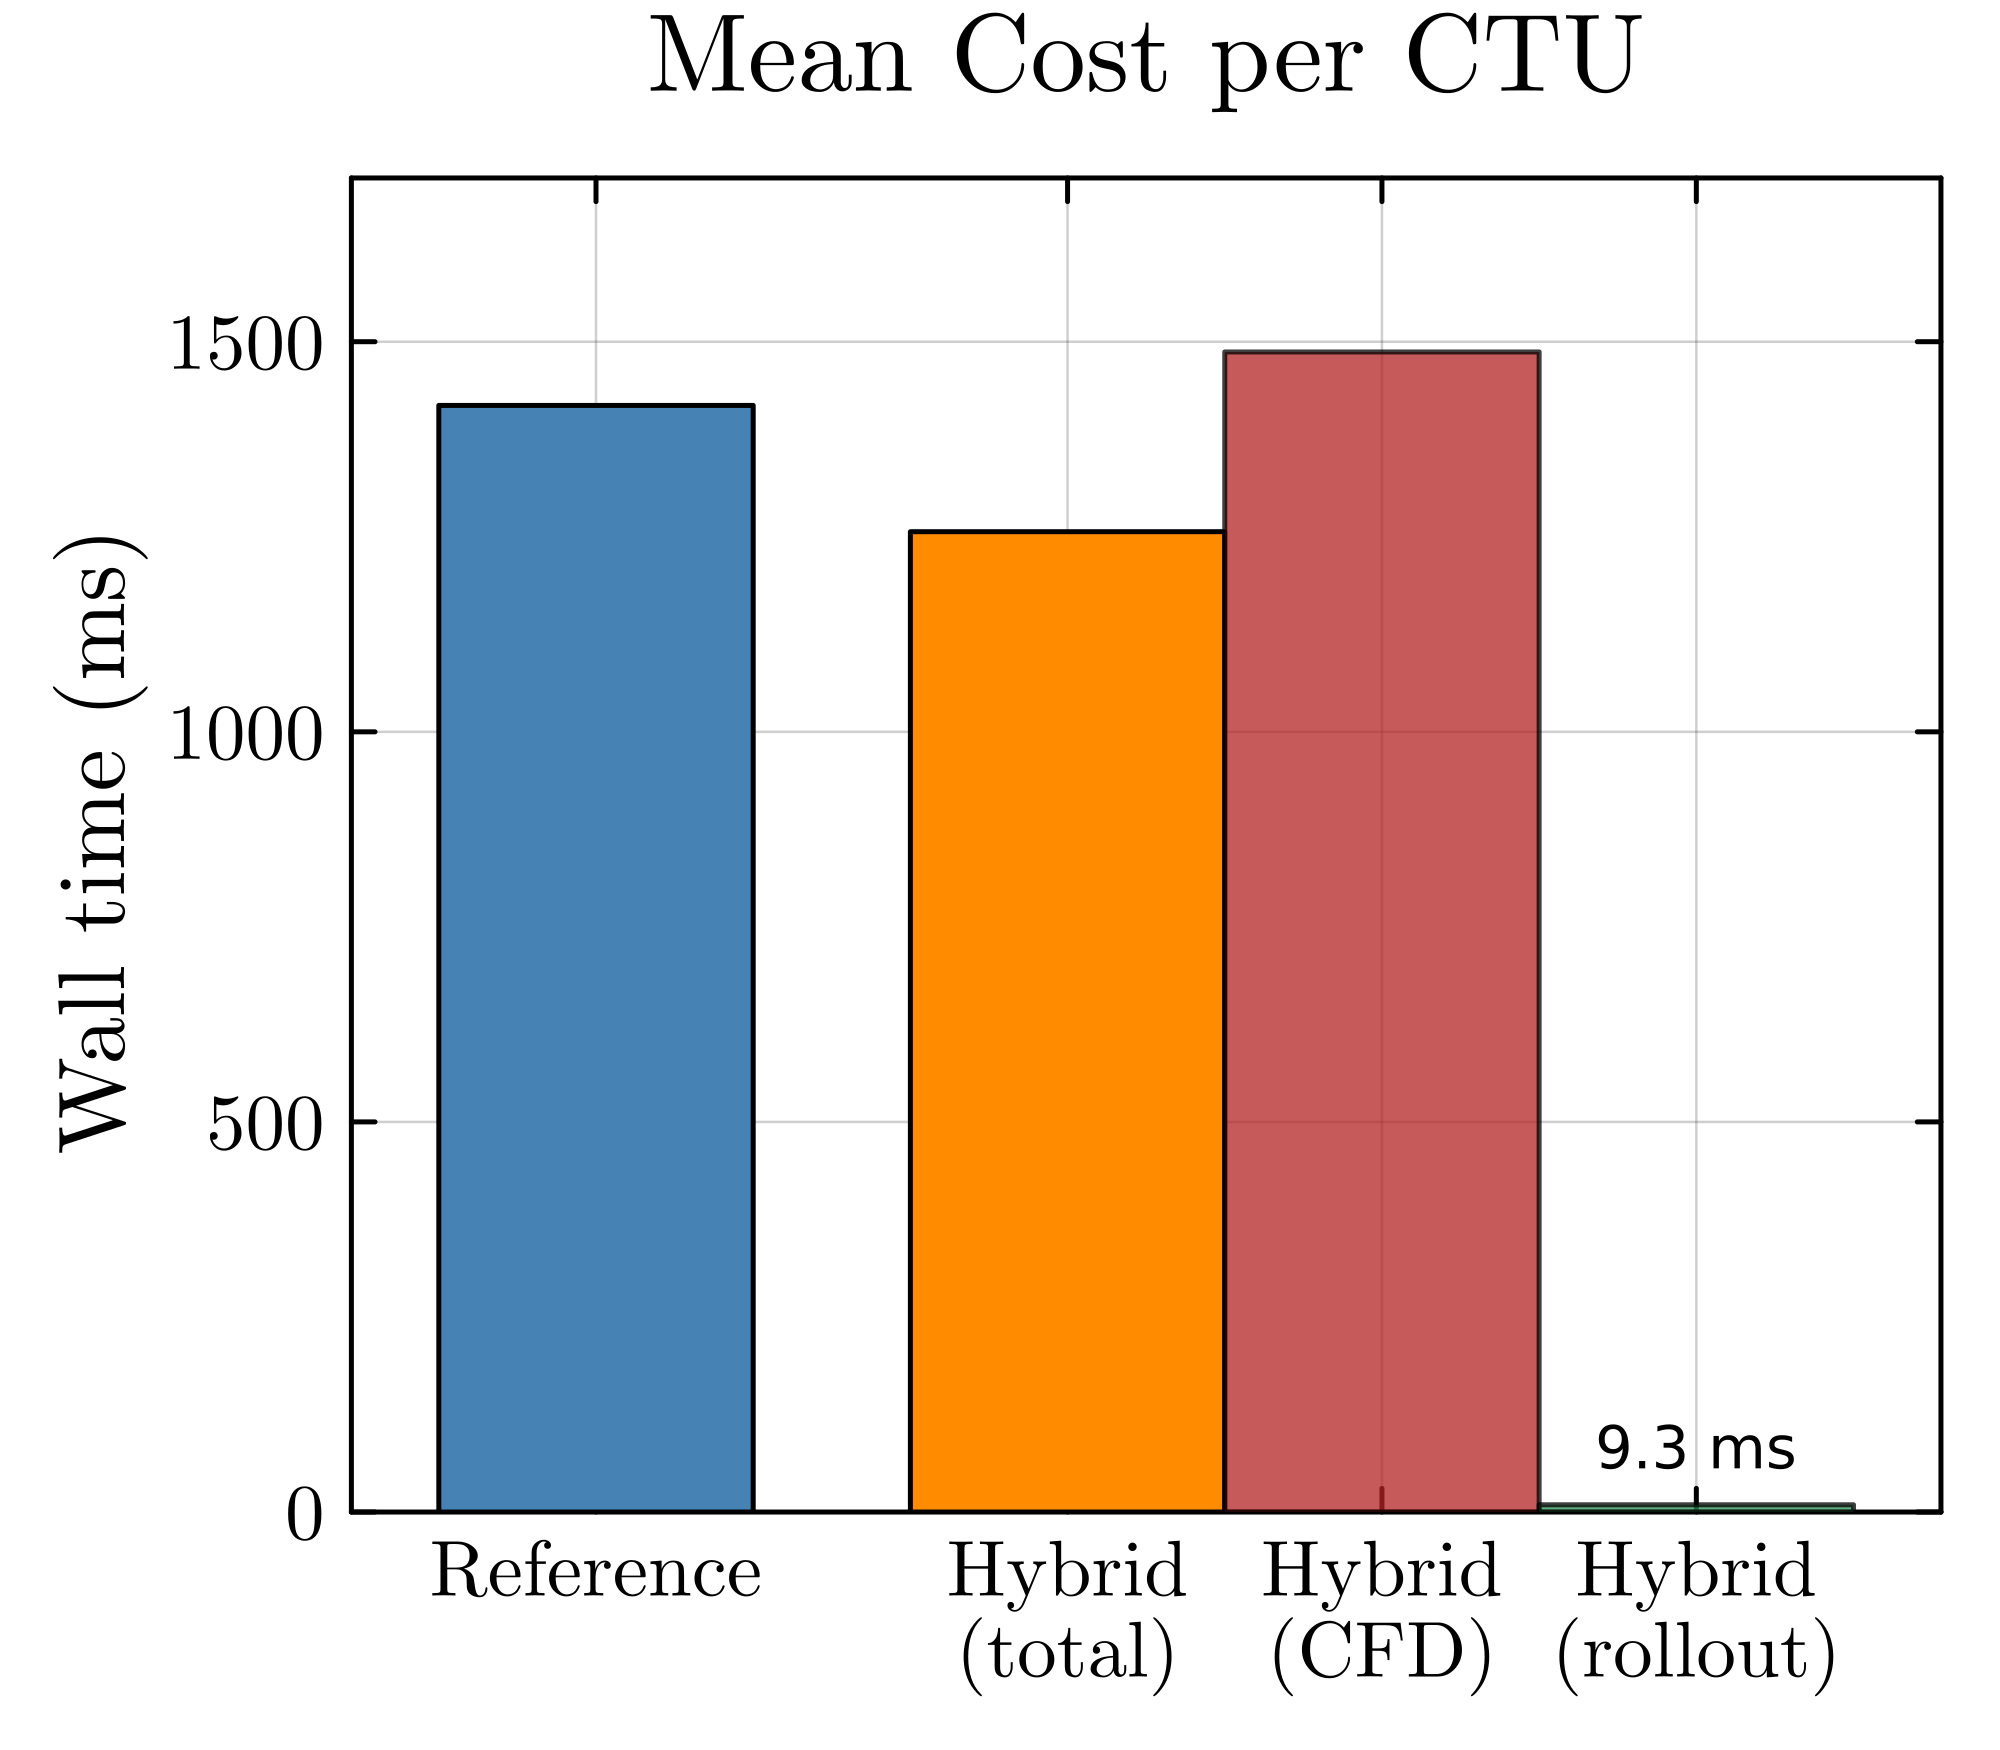
\includegraphics[width=\textwidth]{figures/Results/base/bars_timing.png}
        \caption{Mean wall-time cost per CTU. The hybrid simulation is resolved into its conventional CFD and latent rollout contributions.}
        \label{fig: base_cost_ctu}
    \end{subfigure}
    \hfill
    \begin{subfigure}[t]{0.48\textwidth}
        \centering
        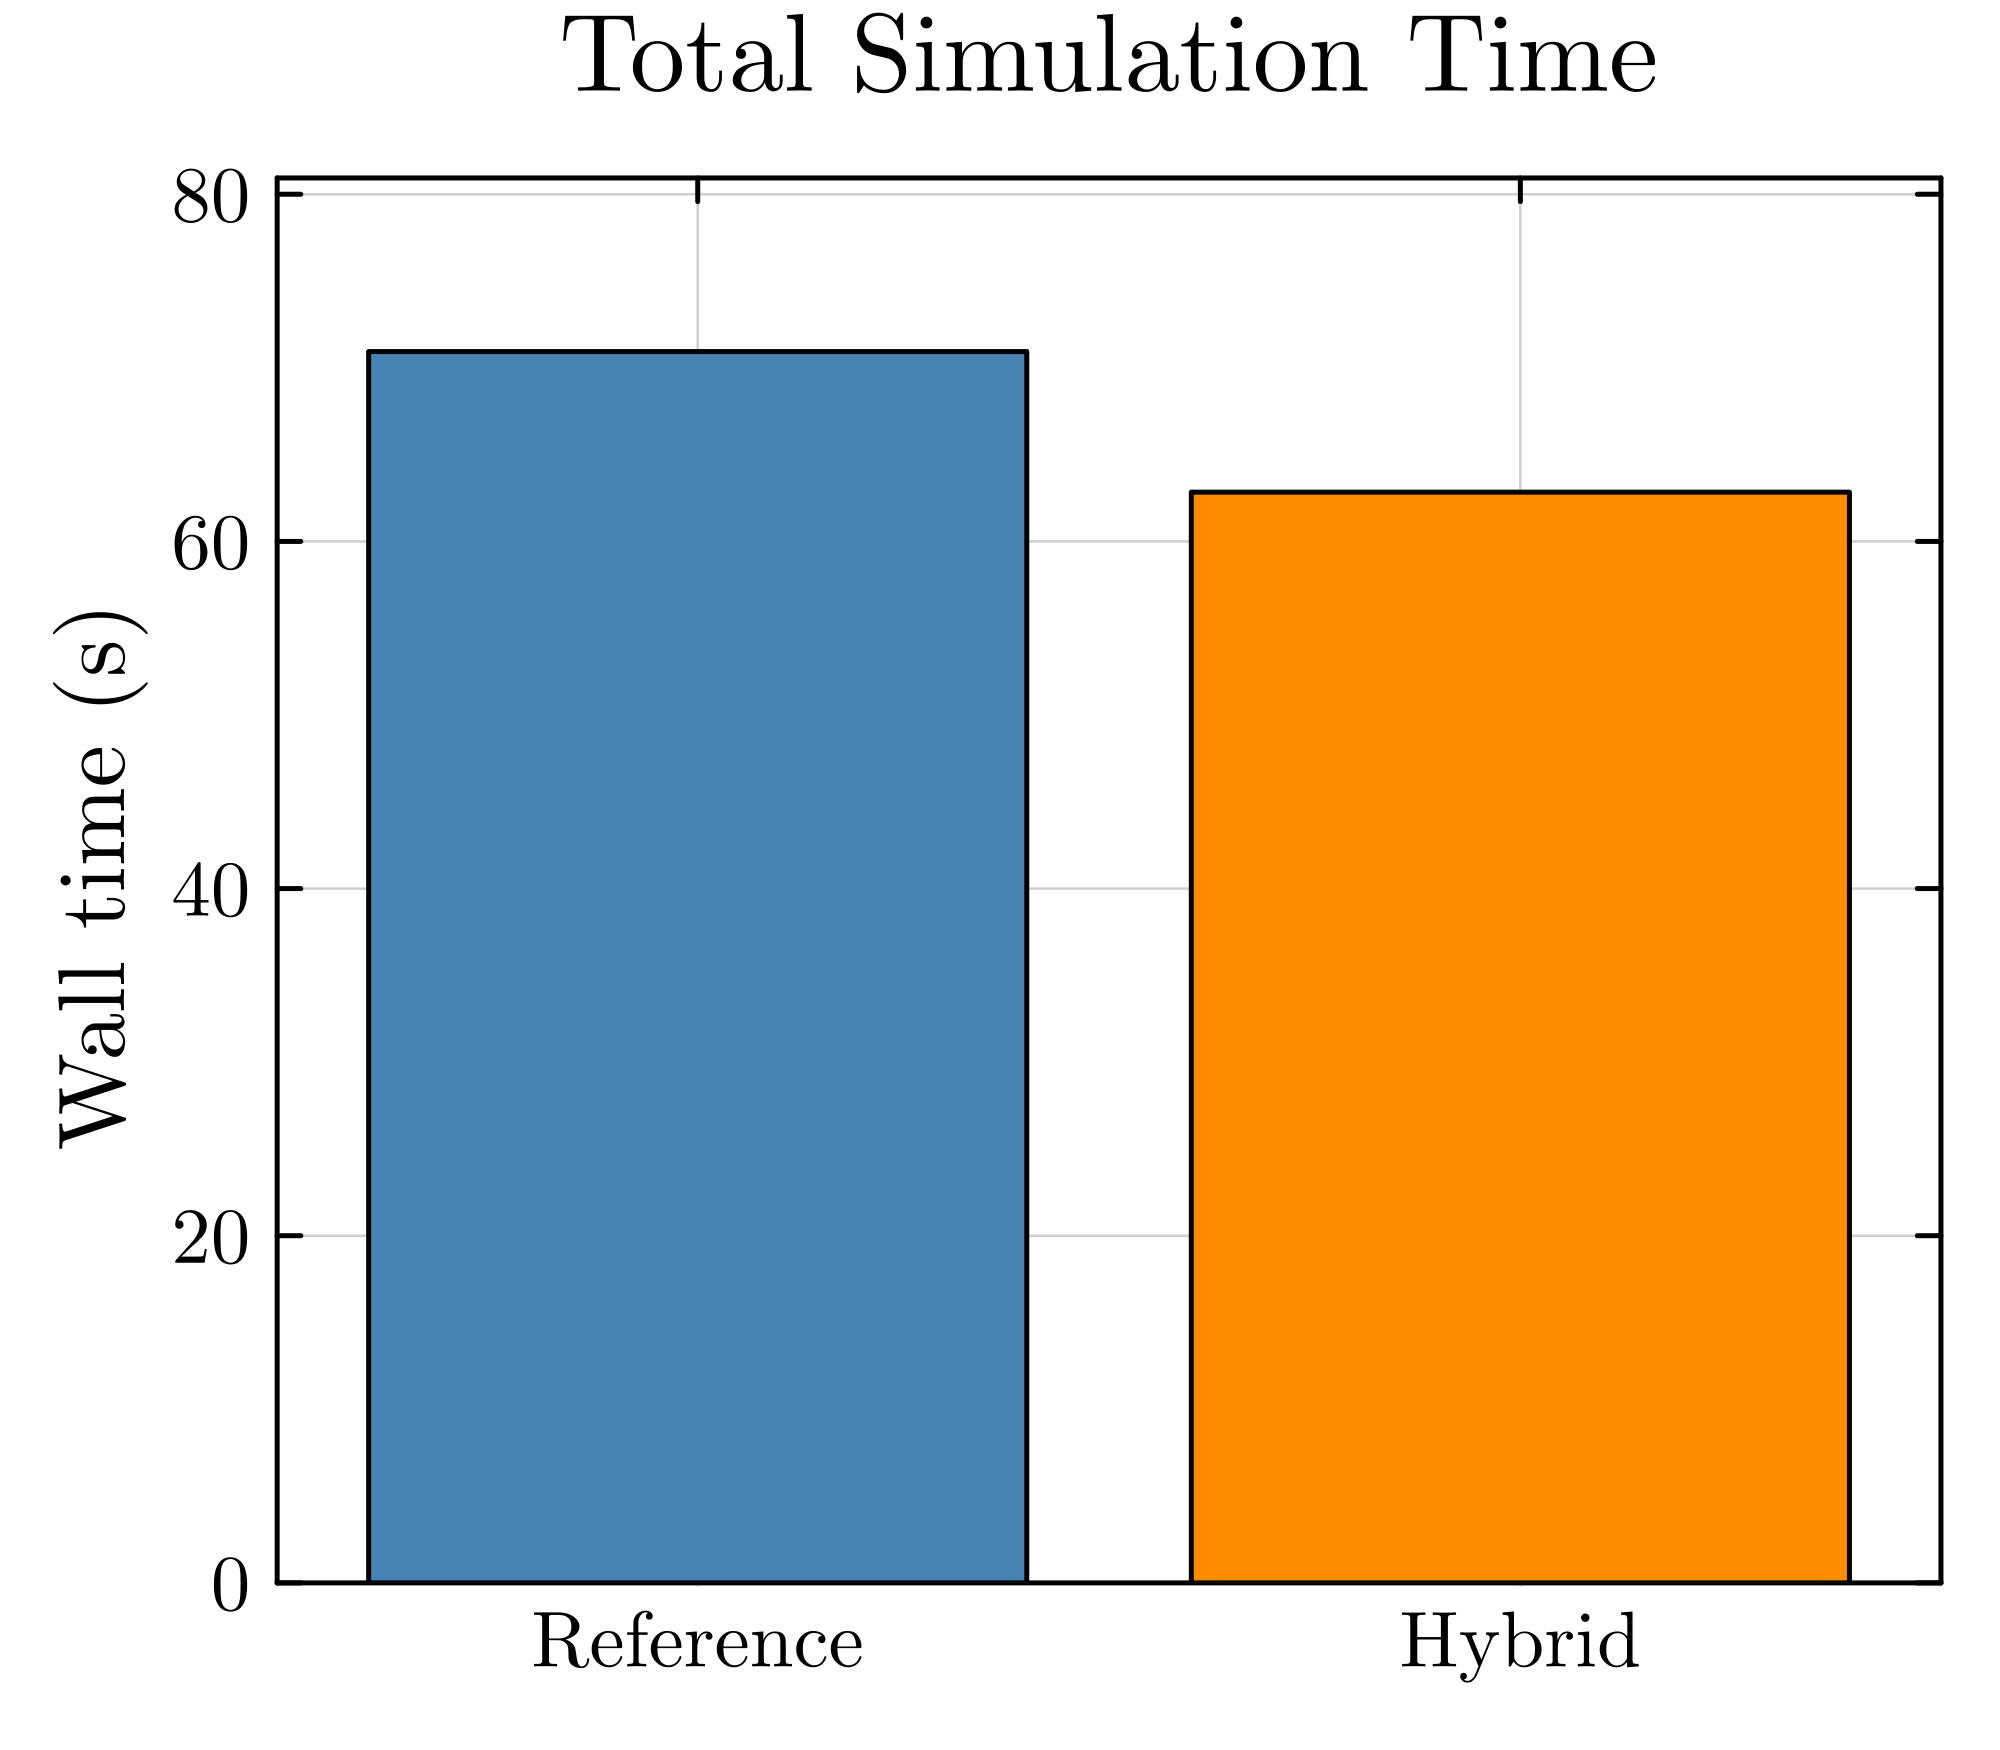
\includegraphics[width=\textwidth]{figures/Results/base/bars_total.png}
        \caption{Total wall time of the hybrid and reference simulation over the same convective-time window.}
        \label{fig: base_cost_total}
    \end{subfigure}
    \caption{Comparison of reference simulation to the hybrid loop in terms of (a) cost per CTU and (b) actual wall time cost}
    \label{fig: hybrid_bars}
\end{figure}

\autoref{fig: hybrid_bars} highlights how cheap a single rollout of $\mathcal{P}$ is compared to regular CFD integration. Using $\mathcal{P}$ to predict a single CTU is $84.6$ times cheaper than calculating the same time window using regular CFD timestepping. This bar chart, however, does not include wall time for the training processes of $\varphi_\theta$, $\psi_\theta$, and $f_\phi$. 

When comparing the total wall time over the same simulation window (\autoref{fig: base_cost_total}), the hybrid loop is able to integrate $\mathcal{S}$ to $t^*_\text{end}$ in $58.85$ seconds compared to $\mathcal{S}_\text{ref}$ integrating the same time window in $86.63$ seconds. Which means the speedup achieved by the hybrid loop can be expressed as:
\begin{equation}
    S_\text{loop} = \frac{T_\text{wall}^\text{ref}}{T_\text{wall}^\text{h, tot}} = \frac{86.63}{58.85} = 1.47
\end{equation}

This value for $S_\text{loop}$ is far below what the per-CTU rollout cost in \autoref{fig: base_cost_ctu} suggests, because the loop still spends most of its time in regular CFD: every rollout is followed by $n_\text{switch} = 150$ CFD steps to stabilise the field, and these steps are slightly more expensive than in the reference run due to the extra encoding and monitoring carried out at each step. The cheap rollout sets the upper bound for the acceleration that the hybrid loop is able to achieve, but the number of rollouts attempted (governed by $n_\text{flag, max}$) and the number of CFD steps between rollouts decide how close the hybrid loop is able to get to this upper bound.

This per-CTU advantage is also specific to the base-case resolution. The WaterLily solver is memory-bound, so its cost per CTU grows with grid size~\cite{Weymouth2025}, whereas the rollout cost is fixed by the latent dimension $N_z = 16$ and is independent of the grid. The ceiling on $S_\text{loop}$ therefore rises at finer resolutions: the present $256^2$ grid is a comparatively cheap case in which to demonstrate the gain, and the relative advantage of the latent rollout would be larger on a grid where CFD is more expensive.


\begin{table}[htp]
    \centering
    \begin{tabular}{llrr}
        \toprule
        \textbf{Phase} & \textbf{Component} & \textbf{Time (s)} &\textbf{ \% of total} \\
        \midrule
        initial data-gathering & -- & 21.16 & 1.80 \\
        \midrule
        \multirow{2}{*}{Train} & AE   & 422.00 & 35.81 \\
                               & NODE & 260.00 & 22.06 \\
        \midrule
        \multirow{3}{*}{Hybrid section 1} & CFD + rollout & 1.17 & 0.10 \\
                                          & CFD + rollout & 1.19 & 0.10 \\
                                          & CFD + rollout & 1.17 & 0.10 \\
        \midrule
        \multirow{3}{*}{Retrain 1} & Gather snapshots & 9.58   & 0.81 \\
                                   & AE               & 66.00  & 5.60 \\
                                   & NODE             & 132.00 & 11.20 \\
        \midrule
        \multirow{3}{*}{Hybrid section 2} & CFD + rollout & 1.18 & 0.10 \\
                                          & CFD + rollout & 1.40 & 0.12 \\
                                          & CFD + rollout & 1.21 & 0.10 \\
        \midrule
        \multirow{3}{*}{Retrain 2} & Gather snapshots & 9.22   & 0.78 \\
                                   & AE               & 66.00  & 5.60 \\
                                   & NODE             & 174.00 & 14.76 \\
        \midrule
        \multirow{3}{*}{Hybrid section 3} & CFD + rollout & 1.16 & 0.10 \\
                                          & CFD + rollout & 1.17 & 0.10 \\
                                          & CFD + rollout & 1.16 & 0.10 \\
        \midrule
        Retrain 3 & Gather snapshots & 7.79 & 0.66 \\
        \midrule
        \textbf{Total} & & \textbf{1,178.56} & \textbf{100.00} \\
        \bottomrule
    \end{tabular}
    \caption{Wall-clock breakdown of the hybrid simulation pipeline (base run).}
    \label{tab: wall_timing_hybrid}
\end{table}

To assess the actual speedup of the complete acceleration workflow, as described in \autoref{sect: acc_workflow}, the wall times of the training procedures of the ML components in $\mathcal{P}$ need to be accounted for. \autoref{tab: wall_timing_hybrid} shows the wall time for the full pipeline, including network training. The initial training dominates: the autoencoder takes $422$ s ($35.81\%$), and the neural ODE $260$ s ($22.06\%$), so building the networks accounts for almost two-thirds of the total time before a single rollout. The three retraining cycles add a further ${\sim}460$ s, while the actual CFD-plus-rollout work contributes less than $1\%$ of the total of $1176.56$~s.


Taking training into account, the effective speedup of the full workflow is
\begin{align}
    S_\text{eff}
    = \frac{T_\text{wall}^\text{ref}}{T_\text{wall}^\text{h, tot} + T_\text{wall}^\text{h, training}}
    = \frac{86.63}{58.56 + 1120}
    \approx 0.073,
\end{align}

This means that for a single hybrid run, the complete workflow is roughly an order of magnitude slower than simply running the reference over the selected window $0 \mapsto t^*_\text{end}$. One of the reasons to put the training times of the autoencoder and the neural ODE in perspective: if training of these models were to happen in parallel, $t^*_\text{handoff}$ would be pushed back by $1018$ CTU, which would put $t^*_\text{handoff}=1038$ CTU. It would be only at this simulation time that the effective cost of $\mathcal{S}$ could be reduced by performing rollout predictions.  

This means that, for a single hybrid run, the complete workflow is roughly an order of magnitude slower than simply running the reference over the selected window $0 \mapsto t^*_\text{end}$. The reason is purely the fixed training cost, over this window the hybrid loop saves $86.63 - 58.85 = 27.78$ s, so a single run would need to integrate for roughly $T_\text{wall}^\text{h, training} / (\text{saving per CTU}) \approx 5000$ CTU before the training cost can be repaid, against the $100$ CTU that were actually integrated. This cost can be recovered only if a trained $\mathcal{P}$ is reused across ${\sim} 50$ comparable runs.

If, as proposed in \autoref{sect: acc_workflow}, training happens parallel to the running simulation $\mathcal{S}$, the handoff time $t^*_\text{handoff}$ would be pushed back significantly. Since the training of the autoencoder and the neural ODE together takes $882$ s, which is equivalent to ${\sim}1018$ CTU of reference integrations. The base window of $100$ CTU is far too short to hide the training behind CFD: the reference run would have finished long before the networks would have finished training.

\subsection{Force Coefficients}
\label{subsect: 4_forces}

\begin{figure}[ht]
    \centering
    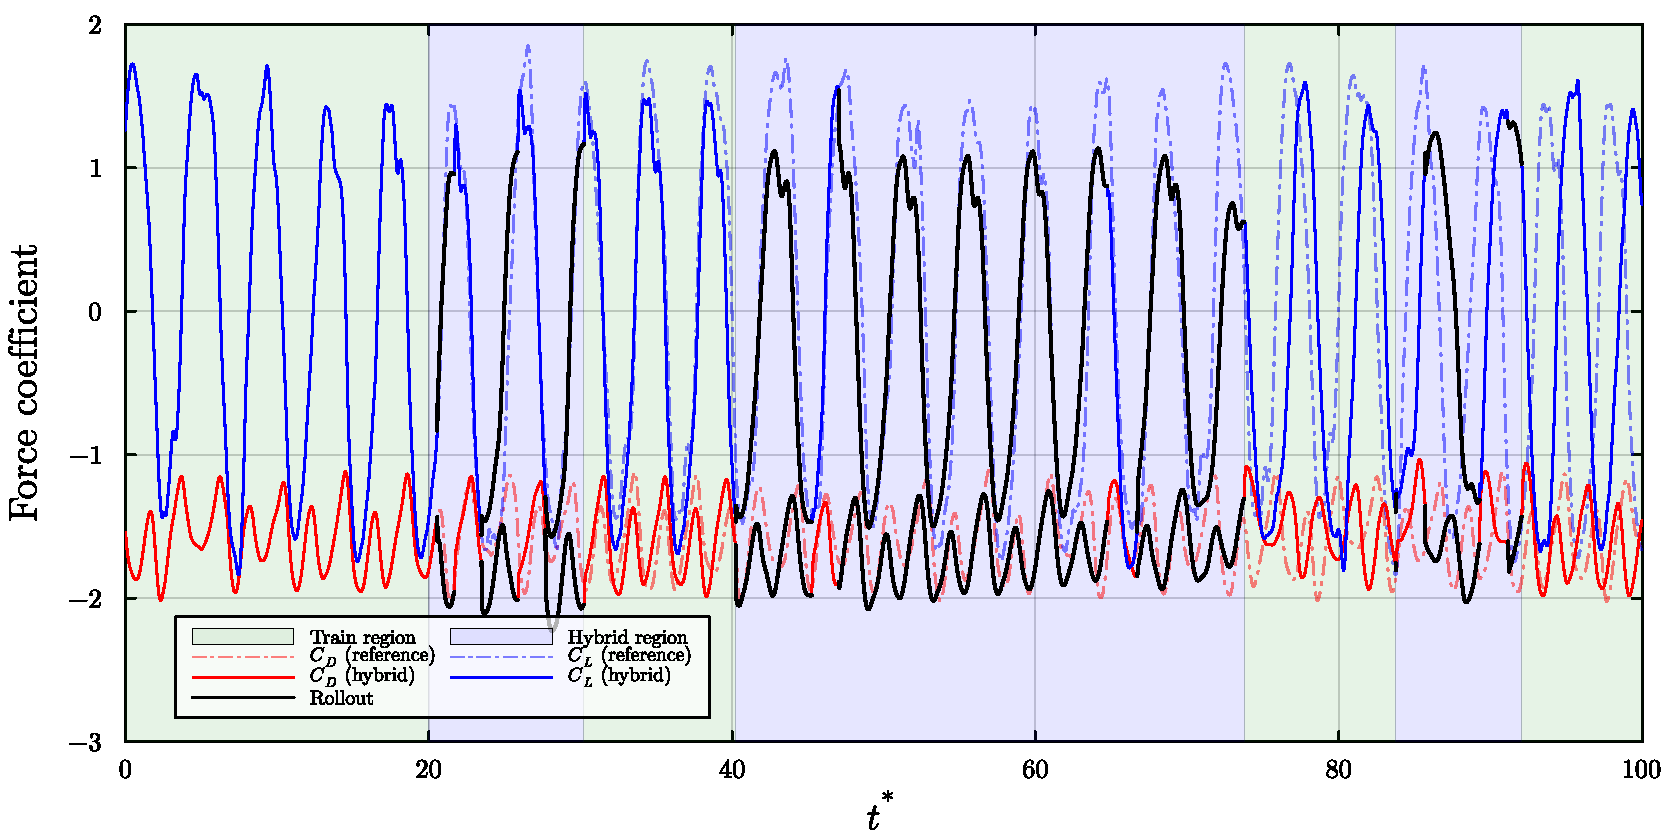
\includegraphics[width=\linewidth]{figures/Results/base/hybrid_forces.pdf}
    \caption{Drag and lift coefficients over time for the reference (dash--dot) and hybrid (solid) simulations, with NODE rollout predictions overlaid (black). Green bands mark pure-CFD intervals (warm-up and retraining); blue bands mark the hybrid windows in which latent rollouts are attempted. Retraining is triggered at $t^* \approx 30.2$, $t^*$, $t^* \approx 73.76$ and $t^* \approx 92.07$}
    \label{fig: base_forces}
\end{figure}

\todo{saturday, fix everything down from here}

Reading \autoref{fig: base_forces} chronologically, following the time axis as in the serial-integrated workflow diagram \autoref{fig: workflow_serial}, the 4 stages of the acceleration workflow are also evident in \autoref{fig: base_forces}. Beginning with the warm-up phase, the hybrid and reference simulations start from a matching initial state at $t^*=0$. From there, both simulations are advanced in time using WaterLily, and instantaneous flow snapshots are saved to disk as training data for $\mathcal{P}$. Having reached $t^*_\text{train}$, the components of $\mathcal{P}$ can be trained; exact loss dynamics of the ML components are reported in \autoref{subsect: 4_ae_performance} and \ref{subsect: 4_node_performance}. After the training procedures, the hybrid loop (\autoref{alg: run_hybrid}) is engaged at $t^*_\text{handoff}=20$ and the first rollouts are attempted. 

The black lines in \autoref{fig: base_forces} trace the pressure force coefficients on the cylinder wall that $\mathcal{P}$ has rolled out and injected back into the simulation. The rollouts track the reference $C_L$ closely at first, but a small phase and amplitude error accumulates as each latent trajectory is integrated further from its initial point; this is the drift that the KNN monitor is designed to catch, and each rollout is cut off just before drifting outside of the known latent distribution range. An example of this drift is visible at the end of the second hybrid window (around $t^* \approx 74$), the hybrid $C_L$ trace has accumulated a visible phase offset relative to the reference, the two signals are no longer in step, and there is a significant amplitude mismatch. Because of the long rollout and the chaotic nature of the wake, a certain amount of divergence is expected and is in itself not an error; however, it places $\mathcal{S}$ on a different point of the shedding cycle than the reference, so the two simulations are no longer pointwise comparable and only their statistical observables remain meaningful. 


To demonstrate that the hybrid simulation accurately reflects the characteristic shedding frequency, the shedding period $T^*$ is measured for each cycle. The period is read directly off the $C_L$ trace of \autoref{fig: base_forces} as the time between successive maxima, and \autoref{fig: base_period_violin} shows the resulting distributions over the complete simulation window. The mean shedding period for the reference and the hybrid simulations is very closely aligned.


\begin{figure}[htbp]
  \centering
  % ---- left: violin plot ----
  \begin{minipage}[c]{0.55\textwidth}
    \centering
    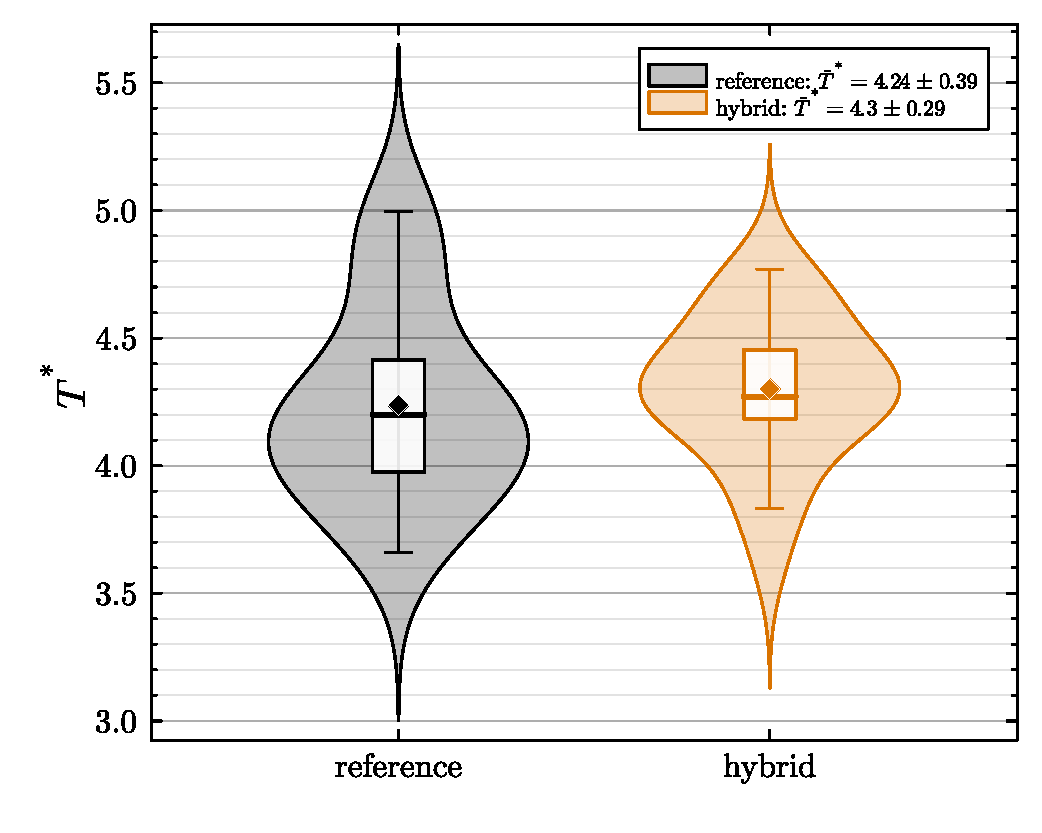
\includegraphics[width=\linewidth]{figures/Results/base/period_violin.pdf}
    \caption{Distribution of the shedding period $T^*$ across the full simulation window for $\mathcal{S}_\text{ref}$ and $\mathcal{S}$, read from successive $C_L$ maxima. Diamonds mark the means; the two distributions overlap within the cycle-to-cycle variance.}
    \label{fig: base_period_violin}
  \end{minipage}\hfill
  % ---- right: Strouhal table ----
  \begin{minipage}[c]{0.42\textwidth}
    \centering
    \vspace{0.5em}
    \begin{tabular}{l
        S[table-format=1.3]
        S[table-format=1.3]
        S[table-format=1.4]}
      \toprule
      & {$\bar{T}^*$} & {$St$} & {$\sigma_{St}$} \\
      \midrule
      Reference & 4.237 & 0.236 & 0.0045 \\
      Hybrid    & 4.301 & 0.233 & 0.0032 \\
      \bottomrule
    \end{tabular}
     \captionof{table}{Mean shedding period $\bar{T}^*$ and Strouhal number $St = 1/\bar{T}^*$ for the reference and hybrid simulations, measured peak-to-peak from the $C_L$ trace. $\sigma_{St}$ is the standard error on the mean.}
    \label{tab: base_strouhal}
  \end{minipage}
\end{figure}

The mean periods are $\bar{T}_\text{ref} = 4.24$ and $\bar{T}_\text{hyb} = 4.30$, giving $St_\text{ref} = 0.236$ and $St_\text{hyb} = 0.233$, a difference of about $1.5\%$ that sits well within the cycle-to-cycle spread of either run. The corresponding Strouhal numbers are shown in \autoref{tab: base_strouhal}. The difference between the reference and hybrid, $\Delta St = 0.0035$, is smaller than the combined standard error on the two means, $\sqrt{\sigma_{St,\text{ref}}^2 + \sigma_{St,\text{hyb}}^2} \approx 0.0055$, showing how there is no meaningful difference between the shedding frequencies of the two
simulations.


The violin plots also show that the hybrid has a smaller variance in the shedding period than the reference. This same behaviour is visible in the second hybrid region of \autoref{fig: base_forces}, where each rolled-out shedding cycle closely matches the others in both amplitude and period, indicating that $\mathcal{P}$ has learned a sort of mean shedding behaviour. The hybrid therefore sheds at the same Strouhal number as the reference, which is consistent with the leading latent components of $f_\phi$ oscillating at the shedding frequency (\autoref{subsect: 4_node_performance}); $\mathcal{P}$ has learned the dominant shedding rhythm correctly rather than a shifted one.

But, as mentioned before, around $t^* \approx 74$ the hybrid $C_L$ trace has accumulated a visible phase offset relative to the reference. \autoref{fig: base_period_violin} shows that the shedding period of $\mathcal{S}$ is very closely aligned to the reference, but it doesn't display where this offset kicks in and what causes it. To view where $\mathcal{S}$ begins to drift, of course, the instantaneous phase of each lift signal is tracked over time using an instantaneous Hilbert transform. The Hilbert transform turns the real, oscillating $C_L$ into a complex signal whose angle is a continuously growing phase $\varphi(t)$; the difference $\Delta\varphi = \varphi_\text{hyb} - \varphi_\text{ref}$, expressed in cycles, can then be assessed to view how much, and where the simulations begin to drift away from each other. 

\begin{figure}[htbp]
    \centering
    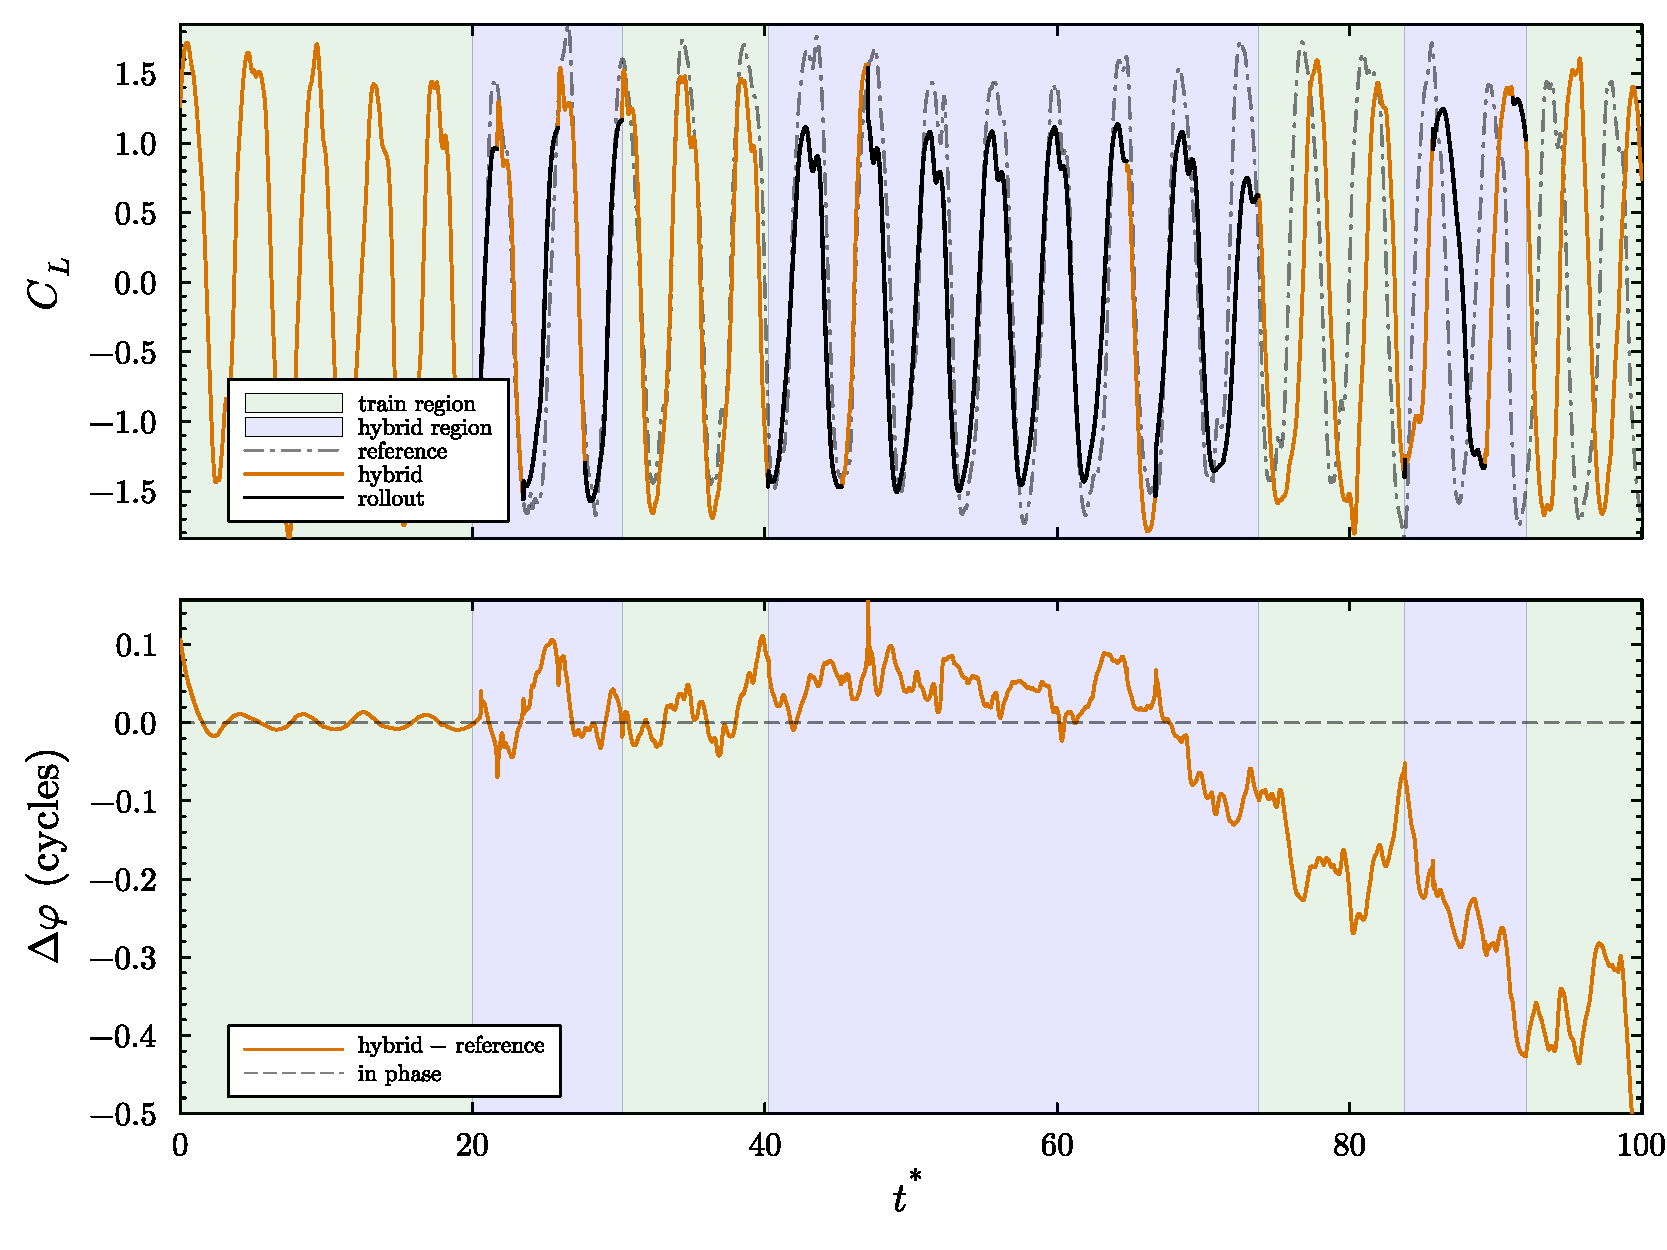
\includegraphics[width=\linewidth]{figures/Results/base/shedding_pase_diff.pdf}
    \caption{Running phase difference $\Delta\varphi = \varphi_\text{hyb} - \varphi_\text{ref}$ of the two lift traces, in cycles. Phase-locked through both hybrid windows, drifting to about $-0.4$ cycle after the final rollout of the second window.}
    \label{fig: base_phase}
\end{figure}


\autoref{fig: base_phase} shows that the two simulations stay decently in phase, within roughly $\pm 0.1$ of a cycle, throughout the first and second rollout regions. Towards the end of the second hybrid region, however, the dissipative behaviour of $\mathcal{P}$ erodes the amplitude of the rolled-out cycles (rollouts~$4$--$6$) and $\mathcal{S}$ no longer tracks the reference, so $\Delta\varphi$ starts to drift away from zero. During the second retrain, the phase difference remains roughly constant, but once the last hybrid region begins, it is pushed further, reaching about $-0.4$ cycles by the end of the run. This renewed drift indicates that the freshly harvested snapshots do not yet represent the current state of $\mathcal{S}$ well enough; $f_\phi$ and $\mathcal{K}$ remain weakly fit to this regime, so each rollout nudges the simulation further off course rather than back towards the reference.

The per-rollout behaviour of the hybrid loop is summarised in \autoref{tab: base_rollout_summary}, listing the number of steps each latent rollout advanced the simulation before the KNN monitor returned control, along with the physical time gained and the score at hand-off.

\begin{table}[htb]
  \centering
  \sisetup{table-number-alignment = center}
  \begin{tabular}{
    c
    l
    S[table-format=3.0]
    S[table-format=2.3]
    S[table-format=2.3]
    S[table-format=1.3]
    S[table-format=1.3]
  }
    \toprule
    {\#} & NODE model & {Steps} & {$\Delta t^*$} & {$t^*_\text{r, end}$} & {KNN score} & {Threshold} \\
    \midrule
    $1$ & initial     & 101  & 1.105 & 21.687 & 0.328 & 0.326 \\
    $2$ & initial     & 217  & 2.373 & 25.869 & 0.329 & 0.326 \\
    $3$ & initial     & 231  & 2.526 & 30.233 & 0.331 & 0.326  \\
    \hline
    $4$ & 1st retrain & 457  & 4.998 & 45.247 & 0.384 & 0.383 \\
    $5$ & 1st retrain & 1615 & 17.664 & 64.740 & 0.387 & 0.383 \\
    $6$ & 1st retrain & 642  & 7.022 & 73.757 & 0.384 & 0.383 \\
    \hline
    $7$ & 2nd retrain & 1    & 0.011 & 83.789 & 0.473 & 0.413 \\
    $8$ & 2nd retrain & 326  & 3.566 & 89.284 & 0.417 & 0.413 \\
    $9$ & 2nd retrain & 82   & 0.897 & 92.075 & 0.414 & 0.413 \\
    \bottomrule
  \end{tabular}
  \caption{Per-rollout summary of the KNN-gated NODE inference. Rollouts~1--3 use the initial NODE; rollouts~4--6 use the retrained NODE (raised KNN threshold). Rollouts~4 and~6 were rejected at the encoder gate after a single step.}
  \label{tab: base_rollout_summary}
\end{table}

\autoref{tab: base_rollout_summary} shows interesting patterns. Firstly, every completed rollout is cut off the moment its KNN score crosses the threshold (rollout~1 at $0.328$ against $0.326$, for example), verifying that the adaptive scheme of \autoref{alg: predict_flex} stops each trajectory at the edge of the known latent distribution. 

Secondly, the length of each rollout varies over the hybrid regions. This variation in rollout length reflects how well the current state of $\mathcal{S}$ is represented in the encoded training trajectories (produced by the trained encoder $\varphi_\theta$) on which $f_\phi$ and the KNN monitor $\mathcal{K}$ have been trained and fit. Since both components draw their logic from the same set of training trajectories $\boldsymbol{\mathcal{T}}_z$, $f_\phi$ can only have learned the dynamics that those trajectories contain, and $\mathcal{K}$ scores any new state by its distance to those same points. If the current state of $\mathcal{S}$ is in a regime that has not been represented by a majority of the states in $\boldsymbol{\mathcal{T}}_z$, it can either serve as a bad initial state for the NODE integration, or it can be in a regime that is not covered by the latent dynamics $f_\phi$. Either possibility will trigger a quick flag from the KNN monitor, resulting in a shorter rollout length.  

The rollout length is therefore a direct reflection of the overlap between the active flow regime and the distribution of latent states in the training trajectories. This is visible in both \autoref{fig: base_forces} and \autoref{tab: base_rollout_summary}, where in the first hybrid region, the neural ODE produces rollouts of mostly similar lengths, showing that it has learned and fit the dynamics of the initial data-gathering CFD steps to a certain confidence, but to produce longer rollouts, more data is needed. In rollouts $4-6$, $f_\phi$ has been updated to produce longer rollouts that stay inside the regime that can be represented by $\boldsymbol{\mathcal{T}}_u$. These longer rollouts also show a gradual decay in oscillation amplitude over their length, indicating that $\mathcal{P}$ has learned a slightly dissipative version of the shedding cycle.

This dissipative behaviour also has a downstream effect. Each of the rollouts $4$--$6$ inject a slightly lower-amplitude field into $\mathcal{S}$ through the coupling routine of \autoref{sect: coupling}; this compounded error accumulates and pushes the simulation into a state that $\boldsymbol{\mathcal{T}}_z$ no longer represents. The subsequent retrain phase attempts to close this gap by augmenting new CFD snapshots to the existing training data $\boldsymbol{\mathcal{T}}_u^{(r+1)}$ as a minority of the snapshots. This means that the bulk of the multiple-shooting loss remains dominated by the older, well-represented dynamics, and the converged weights $\phi^{(r+1)}$ fit the new state only weakly. As a result, both $f_\phi$ and $\mathcal{K}$ remain weakly fit to this regime, so the encoded initial state is a poor starting point for the integration and an immediate KNN trigger. That is why 2 out of 3 rollouts in the last hybrid section are cut short almost as soon as they begin (\autoref{fig: base_forces}), after which the framework resumes data collection to update the network weights. 

The effect of this dissipative behaviour of $\mathcal{P}$ is reflected in \autoref{tab: base_force_error}, where the mean $C_D$ gets conserved compared to the reference simulation, whereas the RMS value of the $C_L$ does appear to show the effects of the dissipative behaviour at the end of the second rollout. 

\begin{table}[htbp]
\centering
\sisetup{table-number-alignment = center}
\begin{tabular}{
  l
  l
  S[table-format=-1.3]
  S[table-format=-1.3]
  S[table-format=1.3]
  S[table-format=2.3]
}
\toprule
 & & \multicolumn{2}{c}{Solution} & \multicolumn{2}{c}{Error} \\
\cmidrule(lr){3-4} \cmidrule(lr){5-6}
Region & Quantity & {Reference} & {Hybrid} & {$e$} & {$e_{\mathrm{rel}}$ [\%]} \\
\midrule
\multirow{2}{*}{Full domain}
  & $\langle C_D \rangle$ & -1.588 & -1.586 & 0.003 & 0.168 \\
  & $C_L^{\mathrm{rms}}$  &  1.185 &  1.144 & 0.041 & 3.479 \\
\addlinespace
\multirow{2}{*}{Hybrid regions}
  & $\langle C_D \rangle$ & -1.582 & -1.582 & 0.003 & 0.169 \\
  & $C_L^{\mathrm{rms}}$  &  1.184 &  1.050 & 0.135 & 11.361 \\
\bottomrule
\end{tabular}
\caption{Time-mean drag, and RMS lift for the reference and hybrid simulations, with absolute error $e$ and relative error $e_\text{rel}$. The full-domain row averages over the whole window $0 \mapsto t^*_\text{end}$; the hybrid-region row restricts the averaging to the intervals in which latent rollouts were active.}
\label{tab: base_force_error}
\end{table}

The mean drag is recovered to within $e_{\mathrm{rel}} \approx 0.17\%$ in both the full domain and the hybrid regions, since $\langle C_D \rangle$ depends only on the first moment of the signal and carries no information about the oscillation amplitude. Where $C_L^{\mathrm{rms}}$, being peak-weighted, is sensitive to amplitude mismatches and shows a lower value for the hybrid simulation during both the whole simulation window, as in the hybrid sections. Over the full computational window, the relative error is $3.48\%$, but when restricting the averaging window to the hybrid regions, it rises to $11.36\%$. The full-domain figure is diluted by the pure-CFD intervals, which track the reference and contribute their undamped lift-coefficient amplitudes to the global RMS. The hybrid-region $C_L^{\mathrm{rms}}$ error is therefore the more faithful measure of error, confirming that the amplitude decay in rollouts $4$--$6$ translates into a measurable loss of lift fluctuation. 


\subsection{Mean Flow and Reynolds-Stress Statistics}
\label{subsect: 4_meanflow_rst}

The force coefficients of \autoref{subsect: 4_forces} certify that the hybrid loop reproduces the \emph{integrated} loading on the body, but they collapse the entire flow onto two scalar time series and therefore say nothing about \emph{where} in the domain the hybrid and reference solutions agree or diverge. Because of the chaotic nature of the cylinder wake at the current Reynolds number, a small perturbation can easily decorrelate hybrid and the reference trajectories. To assess the performance of the accelerated simulation, \autoref{fig: base_meanflow} shows the time-averaged velocity components ($\langle u\rangle, \langle v\rangle$) of the hybrid simulation (right columns) compared to the reference (middle column) and their absolute difference (left column).

\begin{figure}[htbp]
  \centering
  \setlength{\tabcolsep}{0pt}        % no inter-column padding if you switch to tabular
  \captionsetup[subfigure]{skip=1pt} % shrink gap between image and subcaption

    \makebox[0.32\textwidth]{$\mathcal{S}$}
  \makebox[0.32\textwidth]{$\mathcal{S}_\text{ref}$}
  \makebox[0.32\textwidth]{$\bigl| \mathcal{S}-\mathcal{S}_\text{ref}\bigr|$}\par
  \vspace{1pt}
  % --- row 1 ---
    \rotatebox{90}{\makebox[0.33\textwidth][c]{$\langle u\rangle$}}%
  \begin{subfigure}[t]{0.32\textwidth}
    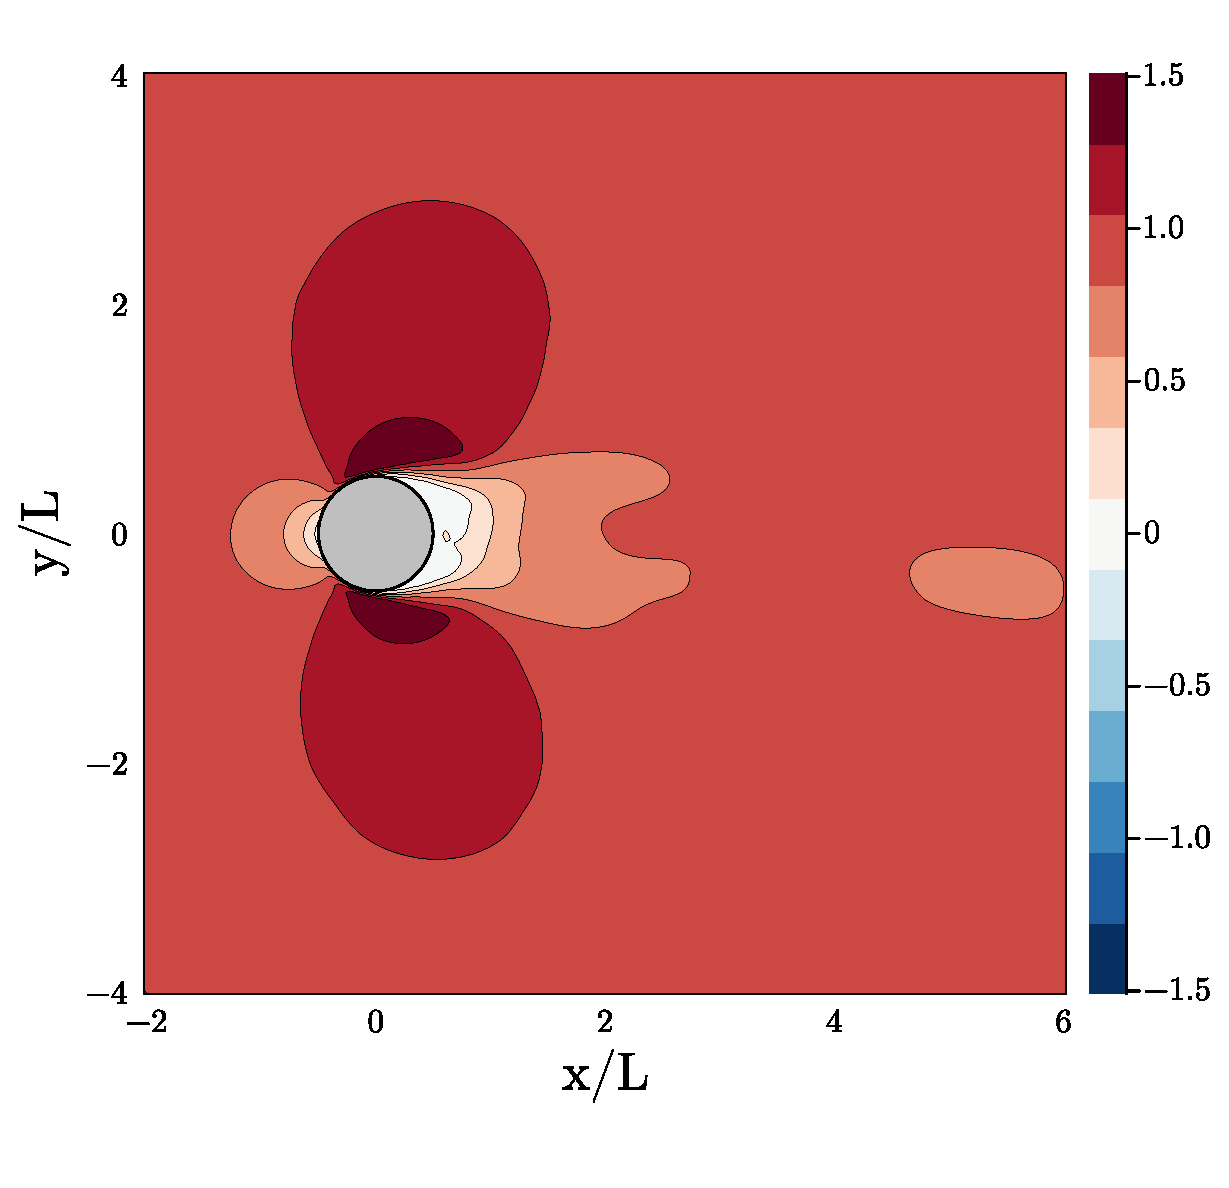
\includegraphics[width=\linewidth]{figures/Results/base/meanflow_panels/meanflow_u_hybrid.pdf}
    \caption{}
    \label{fig: base_hybrid_mean_u}
  \end{subfigure}\hfill
  \begin{subfigure}[t]{0.32\textwidth}
    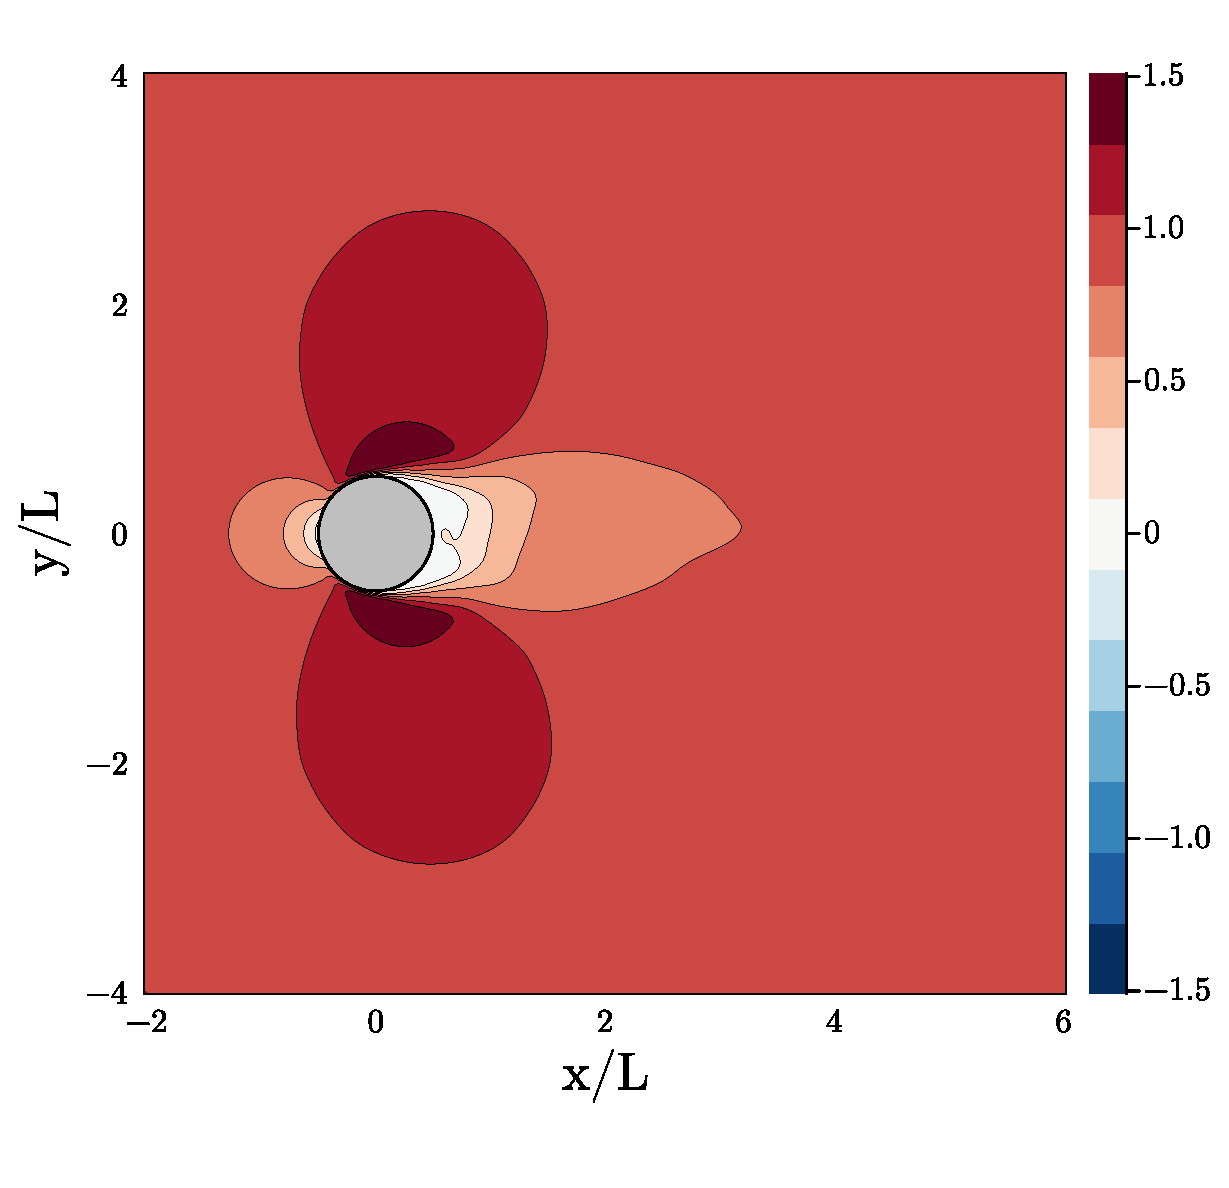
\includegraphics[width=\linewidth]{figures/Results/base/meanflow_panels/meanflow_u_reference.pdf}
    \caption{}
    \label{fig: base_ref_mean_u}
  \end{subfigure}\hfill
  \begin{subfigure}[t]{0.32\textwidth}
    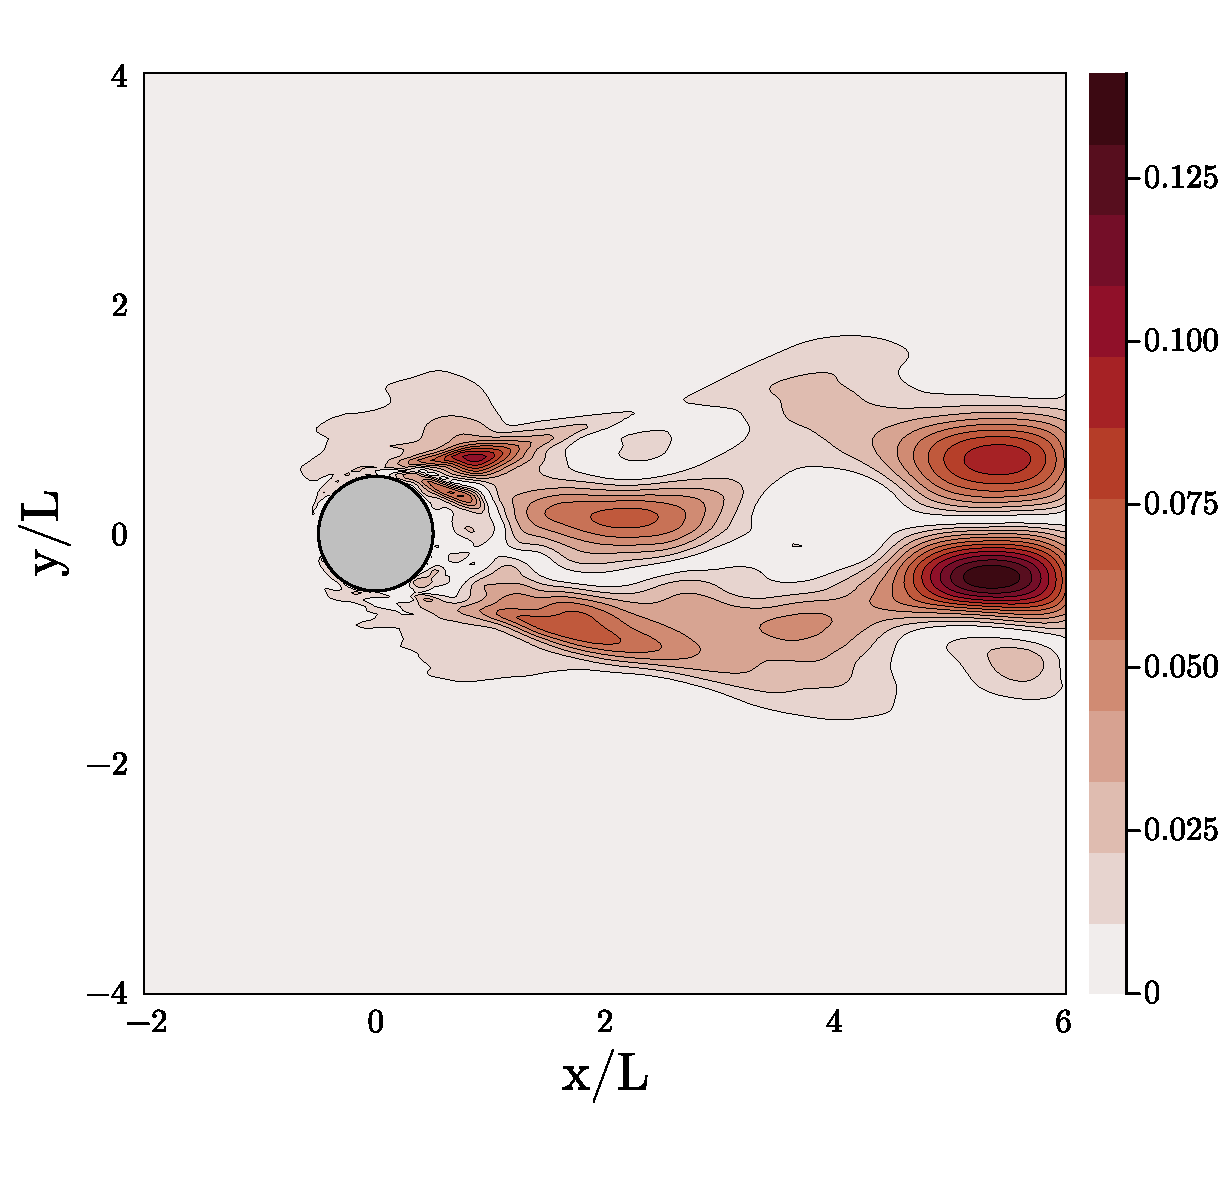
\includegraphics[width=\linewidth]{figures/Results/base/meanflow_panels/meanflow_u_abserror.pdf}
    \caption{}
    \label{fig: base_diff_mean_u}
  \end{subfigure}

  \vspace{-1em} % vertical gap between the two rows; set to 0pt for maximal tightness

  % --- row 2 ---
\rotatebox{90}{\makebox[0.33\textwidth][c]{$\langle v\rangle$}}%
  \begin{subfigure}[t]{0.32\textwidth}
    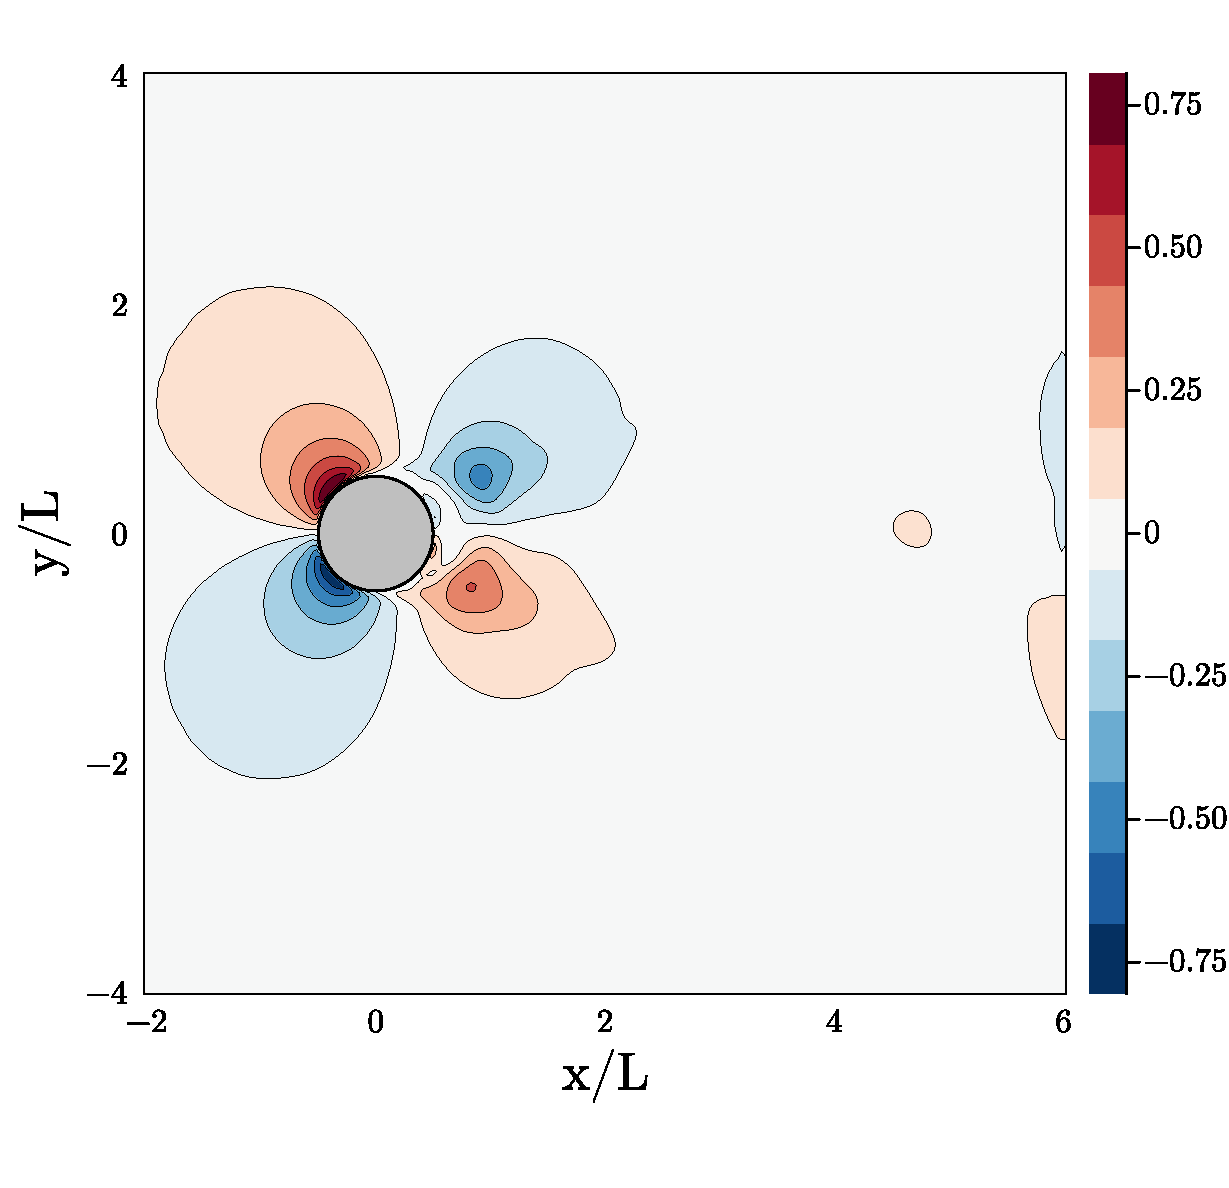
\includegraphics[width=\linewidth]{figures/Results/base/meanflow_panels/meanflow_v_hybrid.pdf}
    \caption{}
    \label{fig: base_hybrid_mean_v}
  \end{subfigure}\hfill
  \begin{subfigure}[t]{0.32\textwidth}
    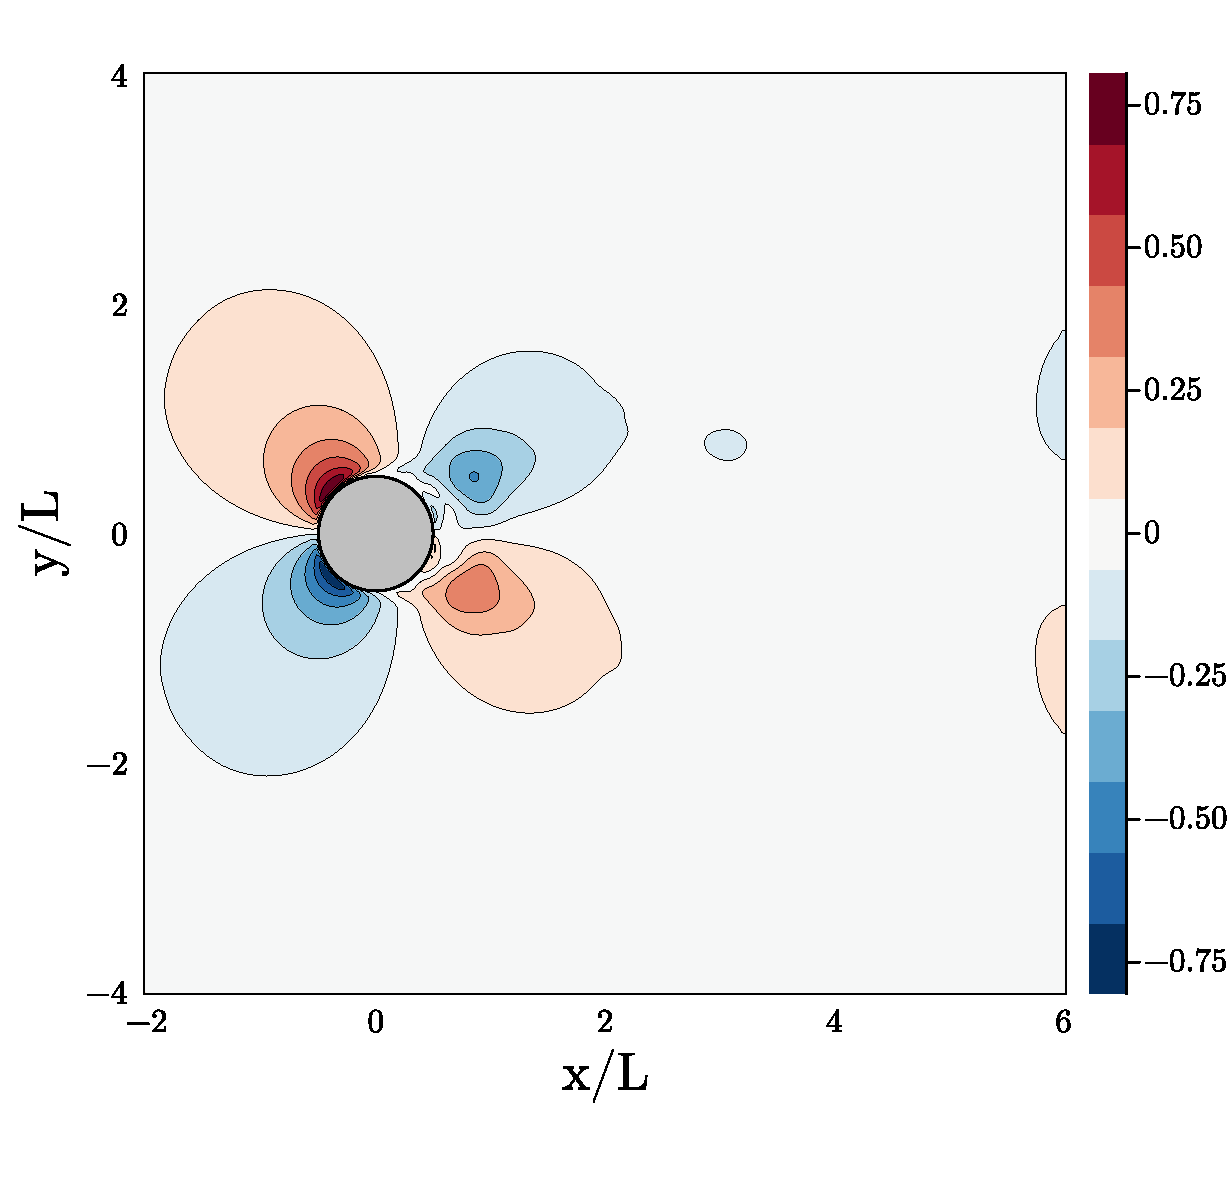
\includegraphics[width=\linewidth]{figures/Results/base/meanflow_panels/meanflow_v_reference.pdf}
    \caption{}
    \label{fig: base_ref_mean_v}
  \end{subfigure}\hfill
  \begin{subfigure}[t]{0.32\textwidth}
    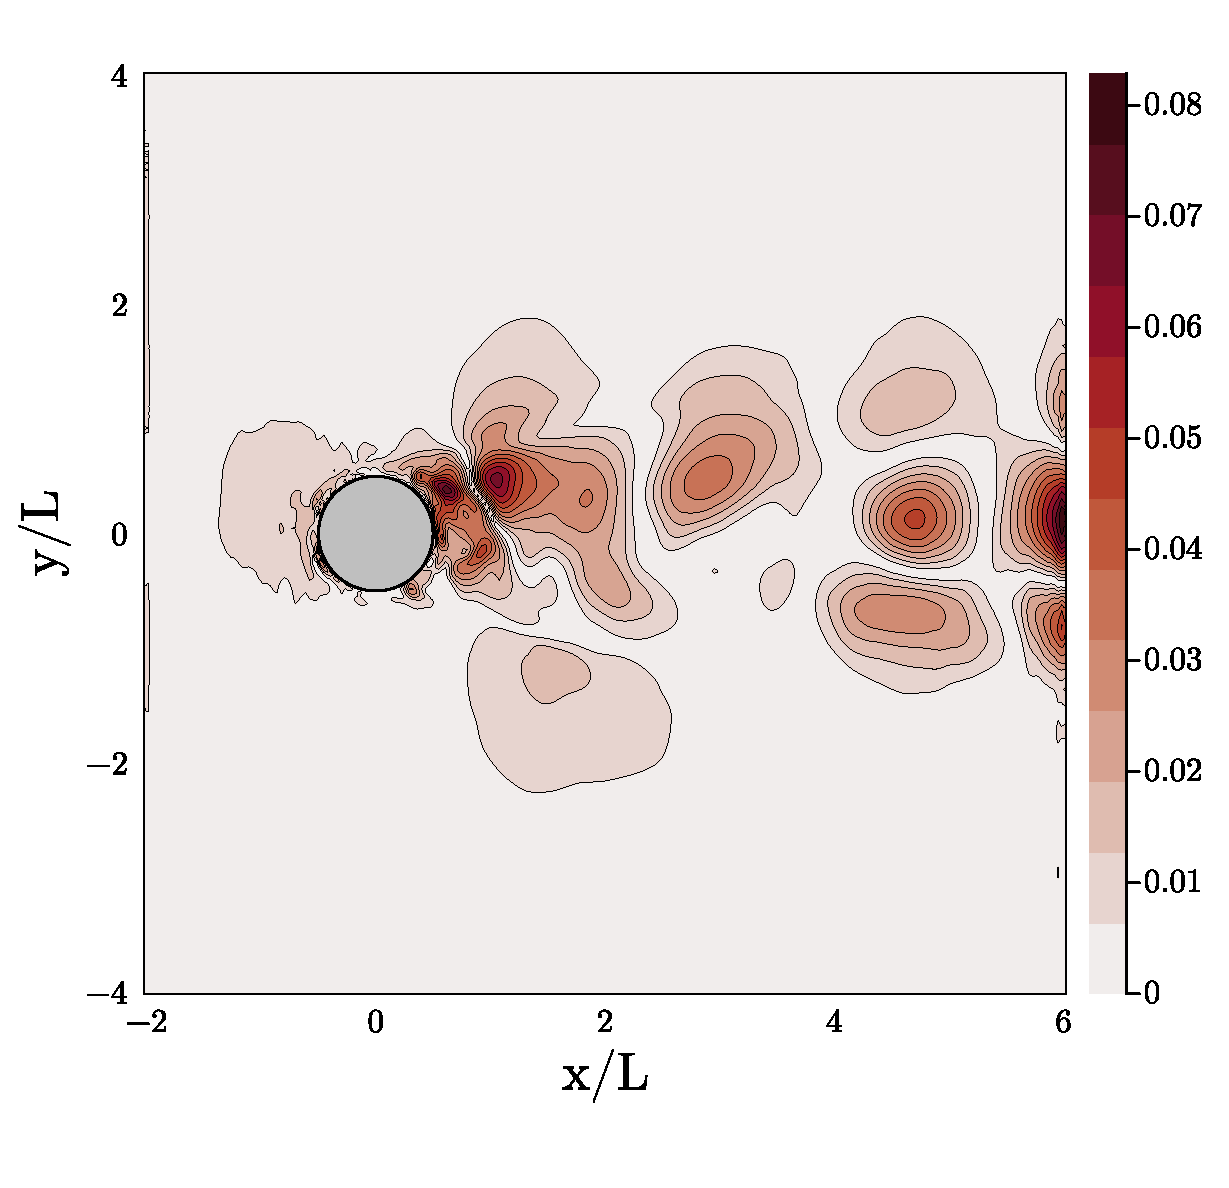
\includegraphics[width=\linewidth]{figures/Results/base/meanflow_panels/meanflow_v_abserror.pdf}
    \caption{}
    \label{fig: base_diff_mean_v}
  \end{subfigure}
\caption{Mean velocity components: $\langle u\rangle$ (top), $\langle v\rangle$ (bottom). Columns: $\mathcal{S}$, $\mathcal{S}_\text{ref}$, absolute difference. Lengths scaled by $L$, velocities by $U$.}
\label{fig: base_meanflow}
\end{figure}


The time-averaged velocity components are computed by sampling instantaneous flow snapshots of $\mathcal{S}$ and $\mathcal{S}_\text{ref}$ at the exact same $t^*$ using a matching sampling interval. Even if the time-dependent properties of $\mathcal{S}$ are different to those of $\mathcal{S}_\text{ref}$, the time-averaged flow fields should produce the same statistics. 

\autoref{fig: base_hybrid_mean_u} and \autoref{fig: base_ref_mean_u} show that both $\langle u\rangle$ have converged in time, showing smooth contours and gradients around the cylinder walls. The only visual difference is in the wake of the cylinder, where the hybrid simulation is less smooth than the reference. \autoref{fig: base_hybrid_mean_v} and \autoref{fig: base_ref_mean_v} also seem to show similar behaviour, where the contours of the mean spanwise flow of the reference are a bit less smooth compared to that of the reference simulation, indicating that the hybrid simulation lacks a small amount of averaging data. 

The absolute-difference fields (\autoref{fig: base_diff_mean_u} \& \autoref{fig: base_diff_mean_v}) show that the discrepancy between the two simulations is negligible over the body and the upstream region and is confined almost entirely to the wake, $x/L \gtrsim 1$. The error peaks at approximately $0.13\,U$ for $\langle u\rangle$ and $0.08\,U$ for $\langle v\rangle$ mostly in the positive spanwise area just behind the cylinder. This matches what could be seen in \autoref{fig: base_forces}, where the rollouts produced lift forces with a lesser amplitude in the positive region of the cylinder wall. This is exactly the region where the most difference between the mean flow components exists. 


\subsubsection{Reynolds Stress Components}

Having computed the time-averaged velocity components, the time-averaged fluctuations of the flow can also be assessed. Using \eqref{eq: ReDecompose}, fluctuating velocity components are extracted and studied to assess the effect of the rollouts on the fluctuating field of $\mathcal{S}$. This allows the three independent components of the Reynolds-stress tensor (RST) to be compared against the reference. Where the normal stresses $\langle u'u'\rangle$ and $\langle v'v'\rangle$ display the energy of the streamwise and transverse fluctuations, and the shear stress $\langle u'v'\rangle$ indicates the momentum transport across the wake.


\begin{figure}[htbp]
  \centering
  \setlength{\tabcolsep}{0pt}
  \captionsetup[subfigure]{skip=1pt}

  % --- column headers ---
  \makebox[0.32\textwidth]{$\mathcal{S}$}
  \makebox[0.32\textwidth]{$\mathcal{S}_\text{ref}$}
  \makebox[0.32\textwidth]{$\bigl| \mathcal{S}-\mathcal{S}_\text{ref}\bigr|$}\par
  \vspace{1pt}

  % --- row 1: <u'u'> ---
  \rotatebox{90}{\makebox[0.30\textwidth][c]{$\langle u'u'\rangle$}}%
  \begin{subfigure}[t]{0.3\textwidth}
    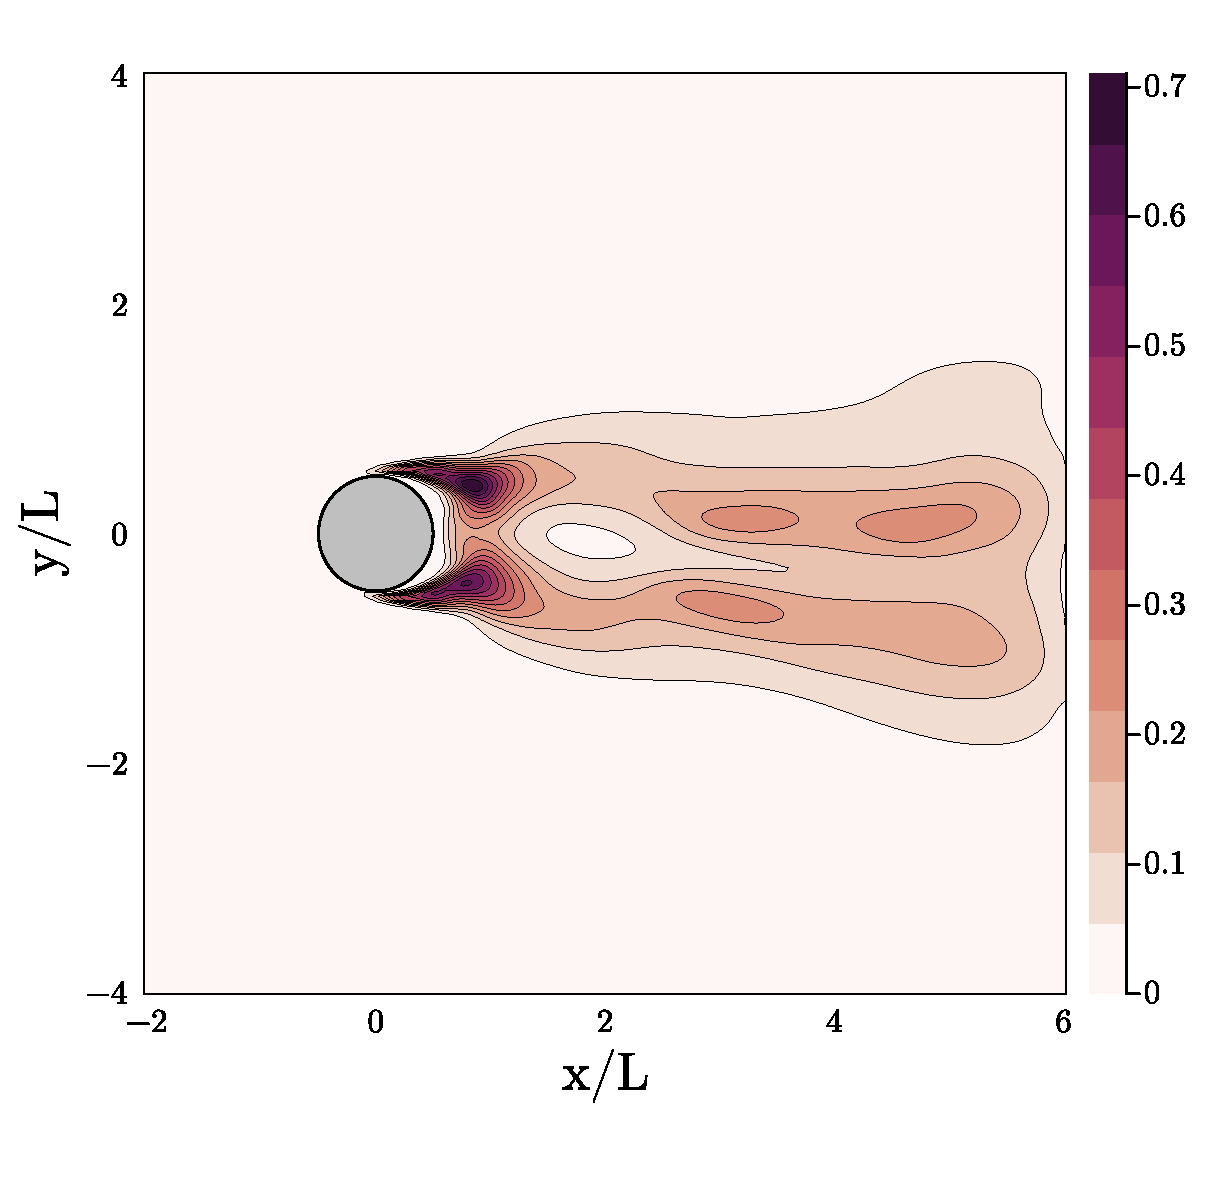
\includegraphics[width=\linewidth]{figures/Results/base/rst_panels/rst_uu_hybrid.pdf}
    % \caption{}
    \label{fig: base_rst_uu_hybrid}
  \end{subfigure}
  \begin{subfigure}[t]{0.3\textwidth}
    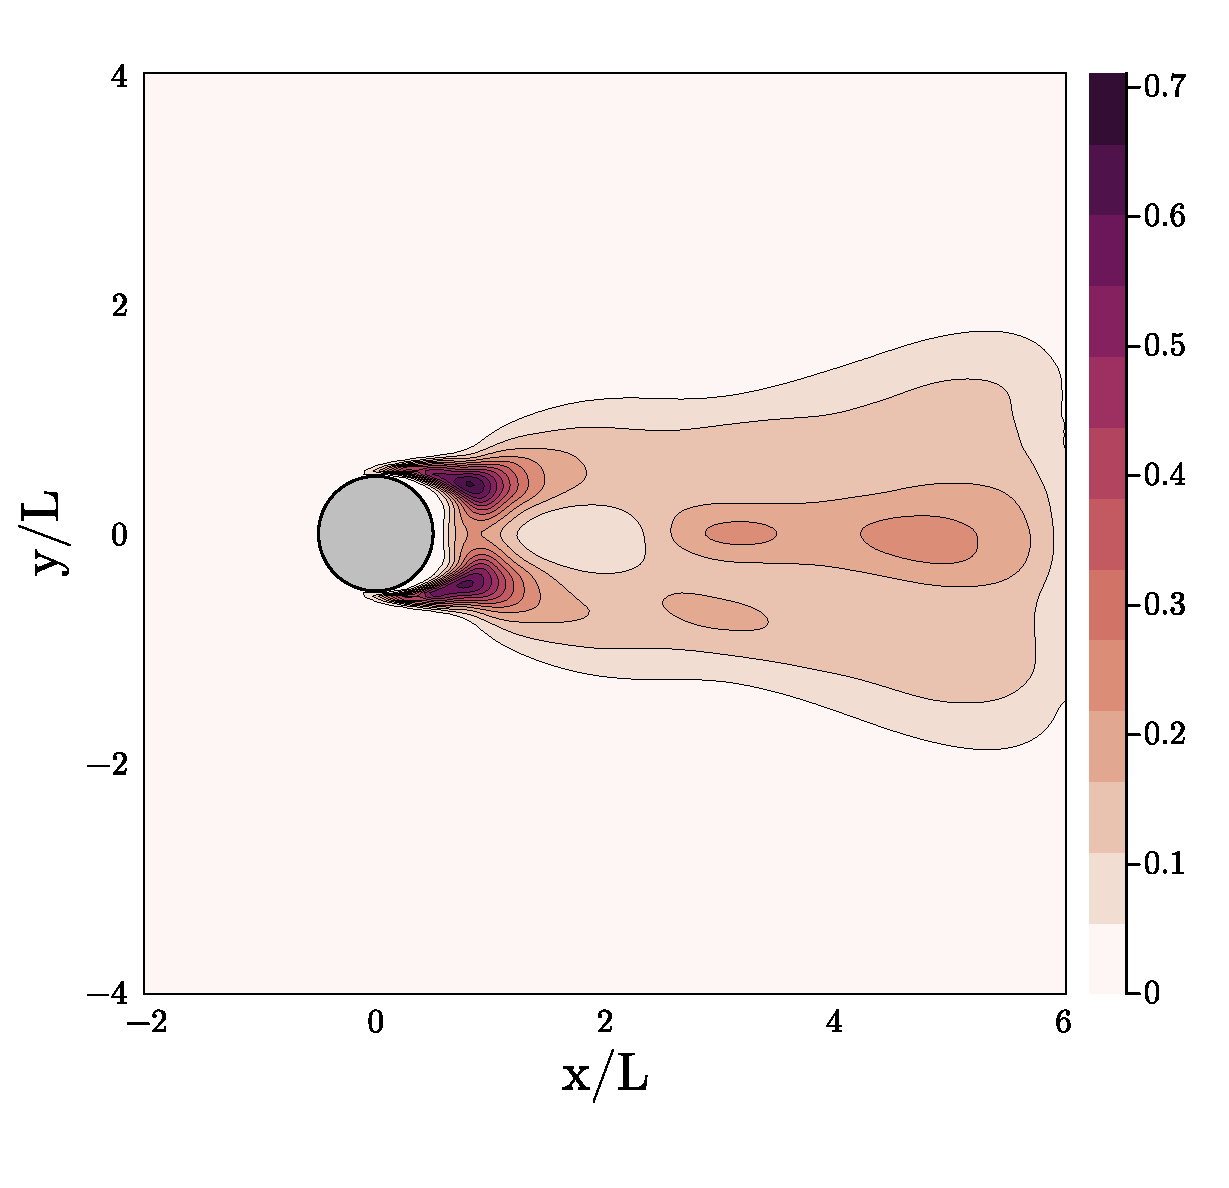
\includegraphics[width=\linewidth]{figures/Results/base/rst_panels/rst_uu_reference.pdf}
    % \caption{}
    \label{fig: base_rst_uu_ref}
  \end{subfigure}
  \begin{subfigure}[t]{0.3\textwidth}
    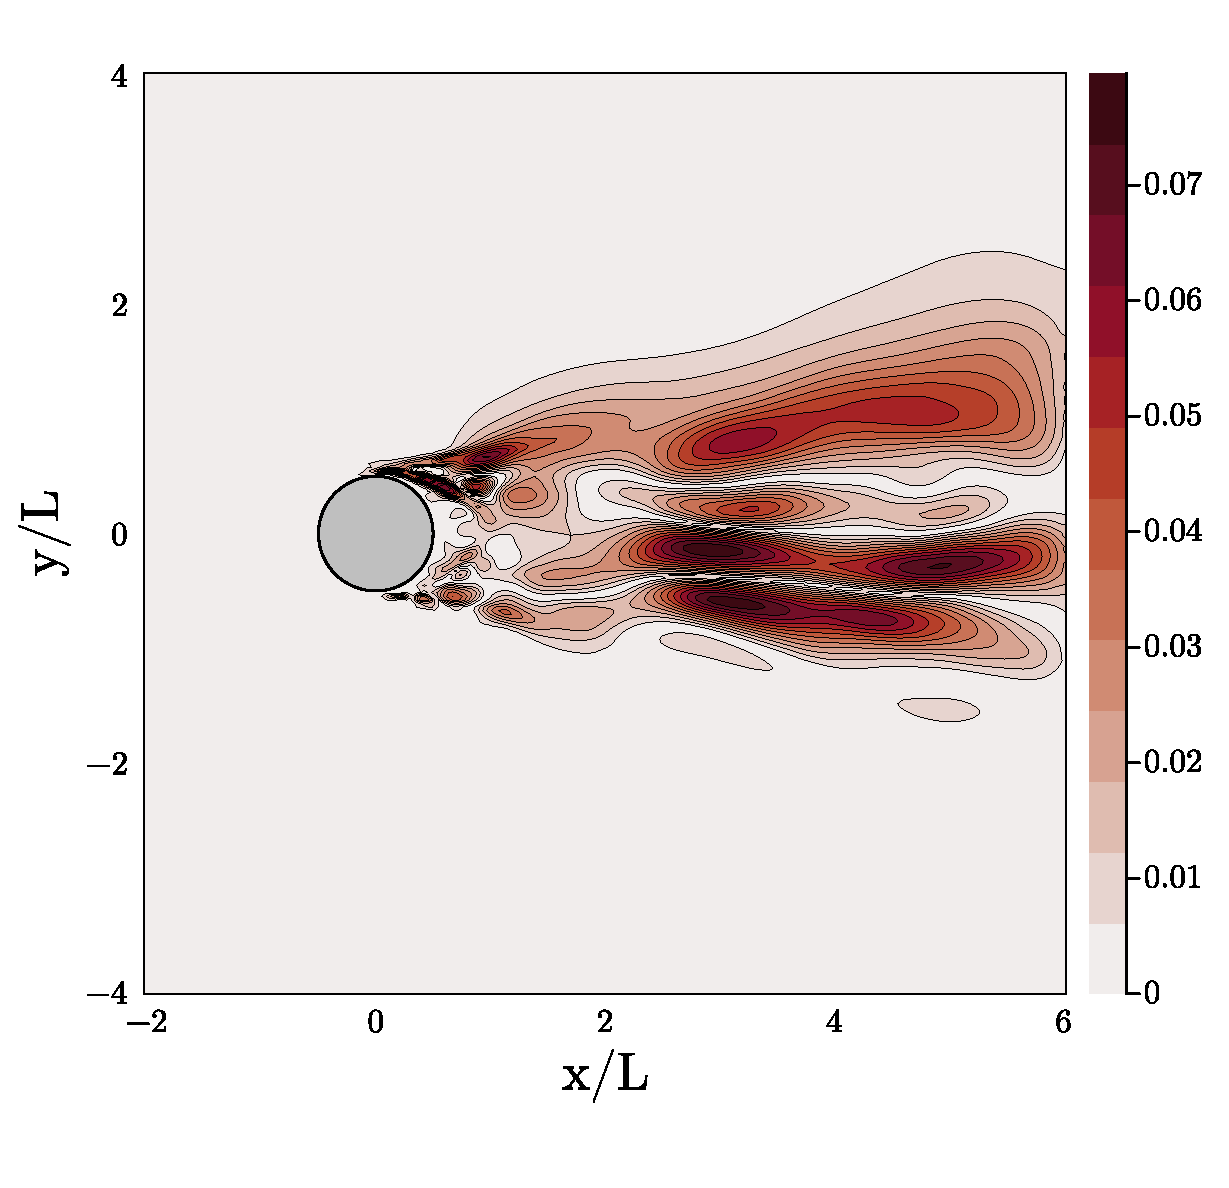
\includegraphics[width=\linewidth]{figures/Results/base/rst_panels/rst_uu_abserror.pdf}
    % \caption{}
    \label{fig: base_rst_uu_diff}
  \end{subfigure}

  \vspace{-2em}

  % --- row 2: <v'v'> ---
  \rotatebox{90}{\makebox[0.30\textwidth][c]{$\langle v'v'\rangle$}}%
  \begin{subfigure}[t]{0.3\textwidth}
    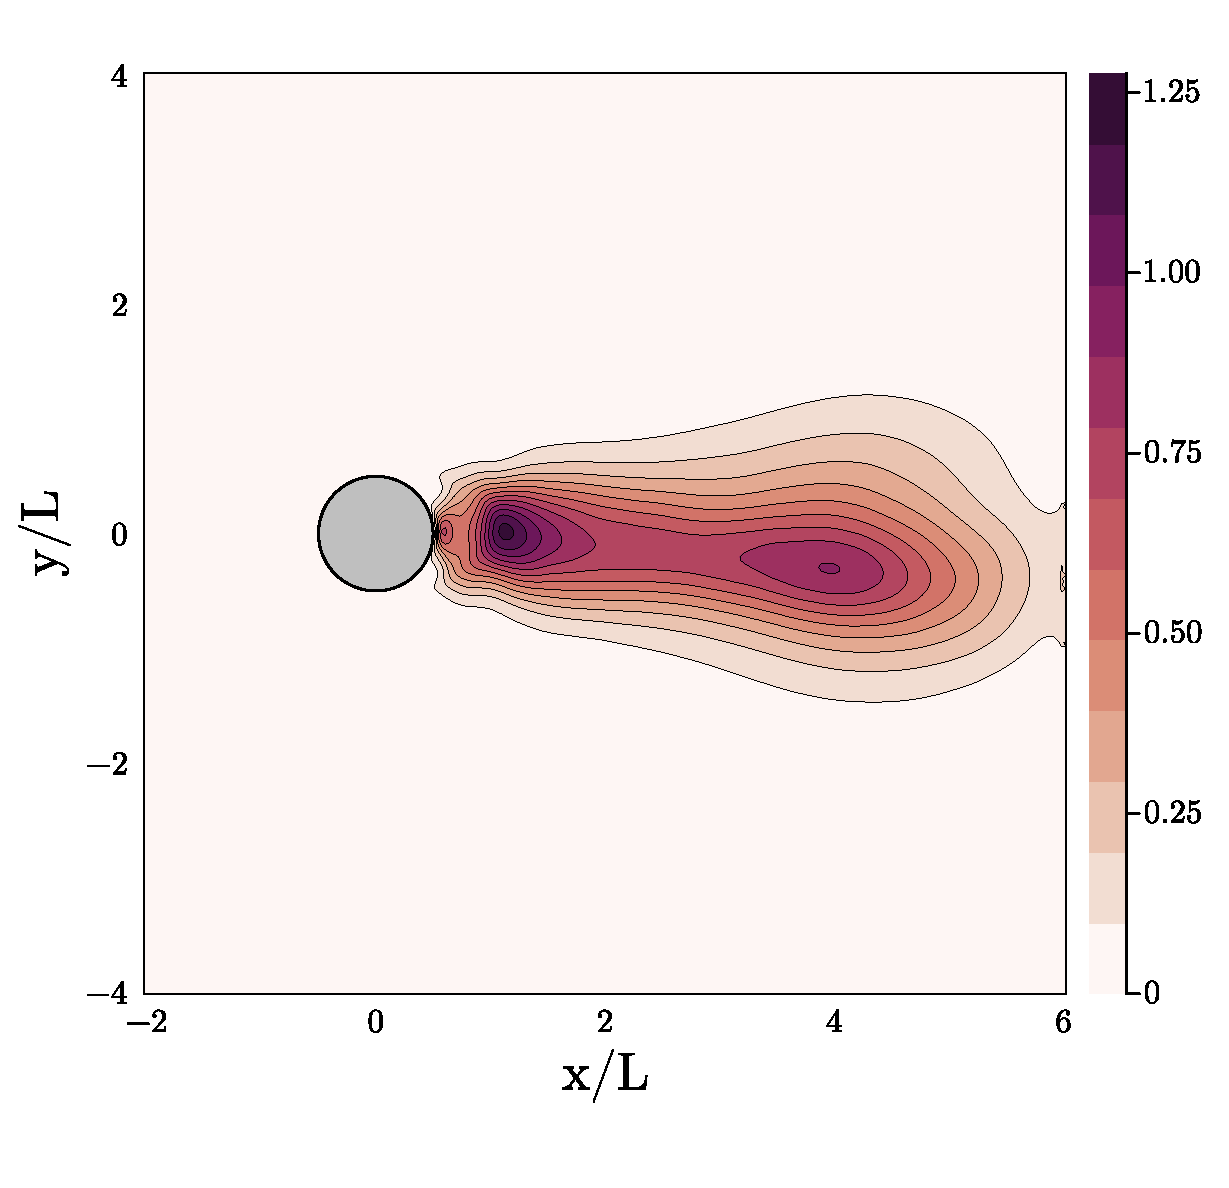
\includegraphics[width=\linewidth]{figures/Results/base/rst_panels/rst_vv_hybrid.pdf}
    % \caption{}
    \label{fig: base_rst_vv_hybrid}
  \end{subfigure}
  \begin{subfigure}[t]{0.3\textwidth}
    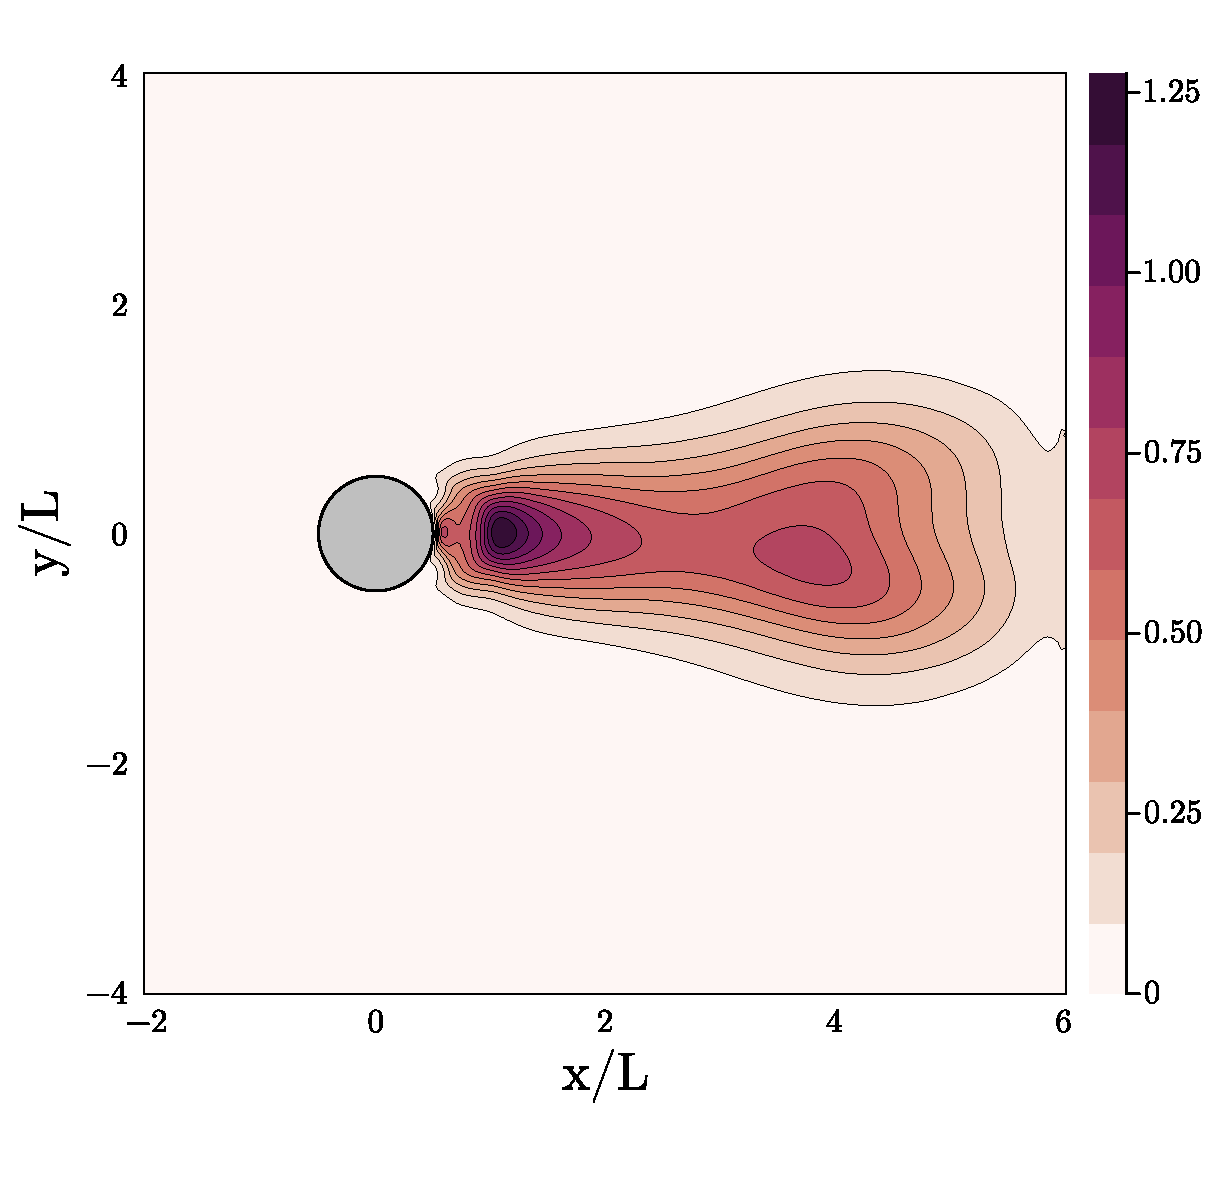
\includegraphics[width=\linewidth]{figures/Results/base/rst_panels/rst_vv_reference.pdf}
    % \caption{}
    \label{fig: base_rst_vv_ref}
  \end{subfigure}
  \begin{subfigure}[t]{0.3\textwidth}
    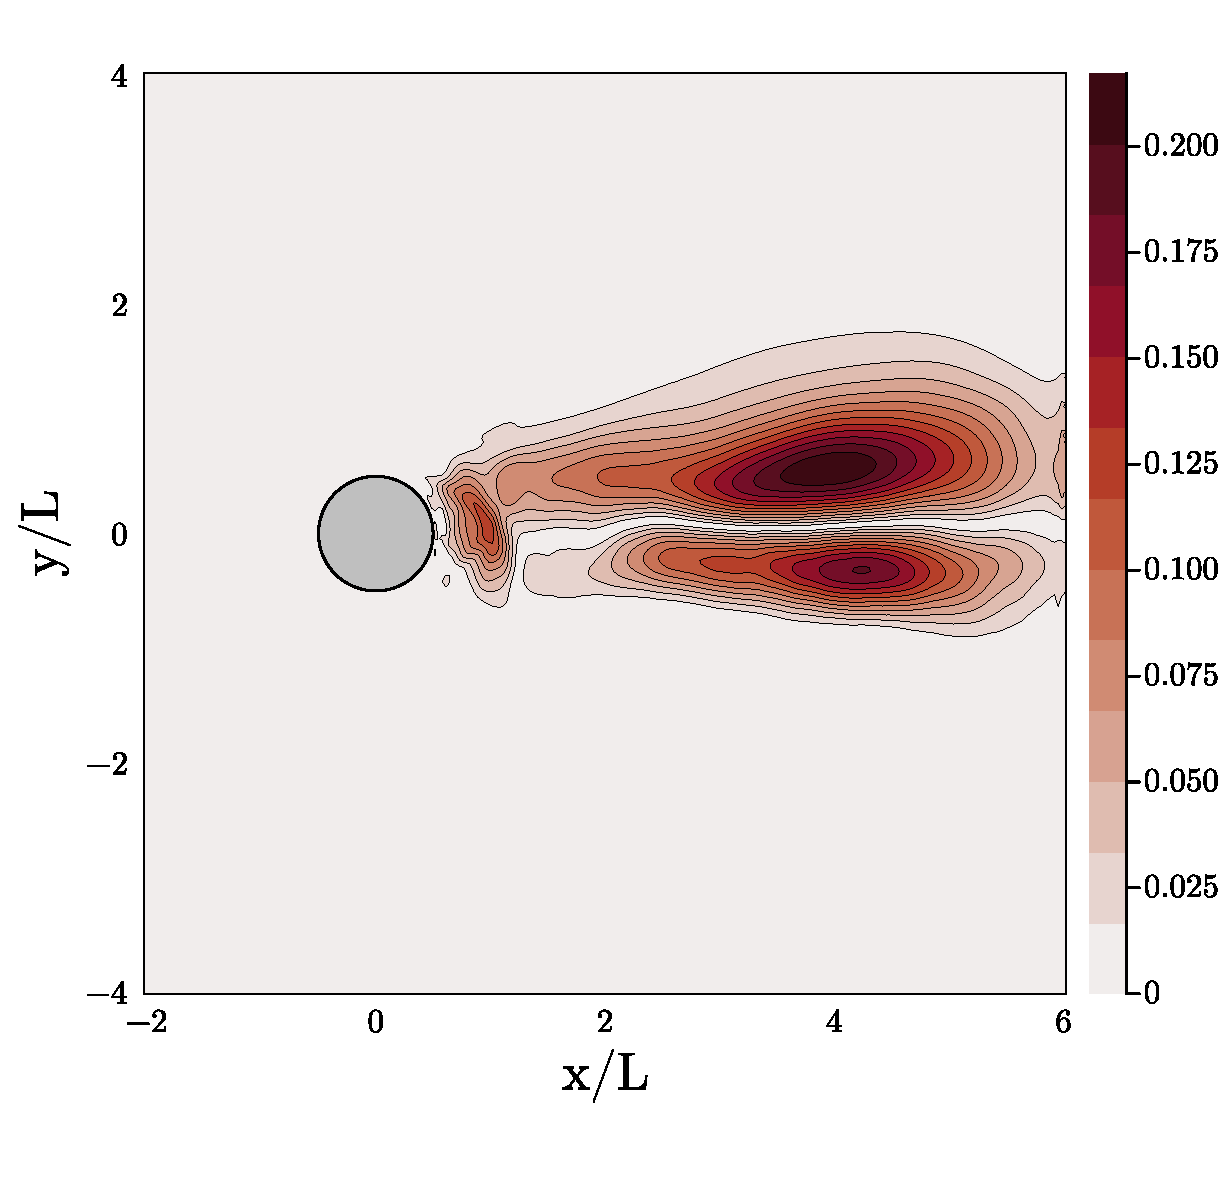
\includegraphics[width=\linewidth]{figures/Results/base/rst_panels/rst_vv_abserror.pdf}
    % \caption{}
    \label{fig: base_rst_vv_diff}
  \end{subfigure}

  \vspace{-2em}

  % --- row 3: <u'v'> ---
  \rotatebox{90}{\makebox[0.30\textwidth][c]{$\langle u'v'\rangle$}}%
  \begin{subfigure}[t]{0.3\textwidth}
    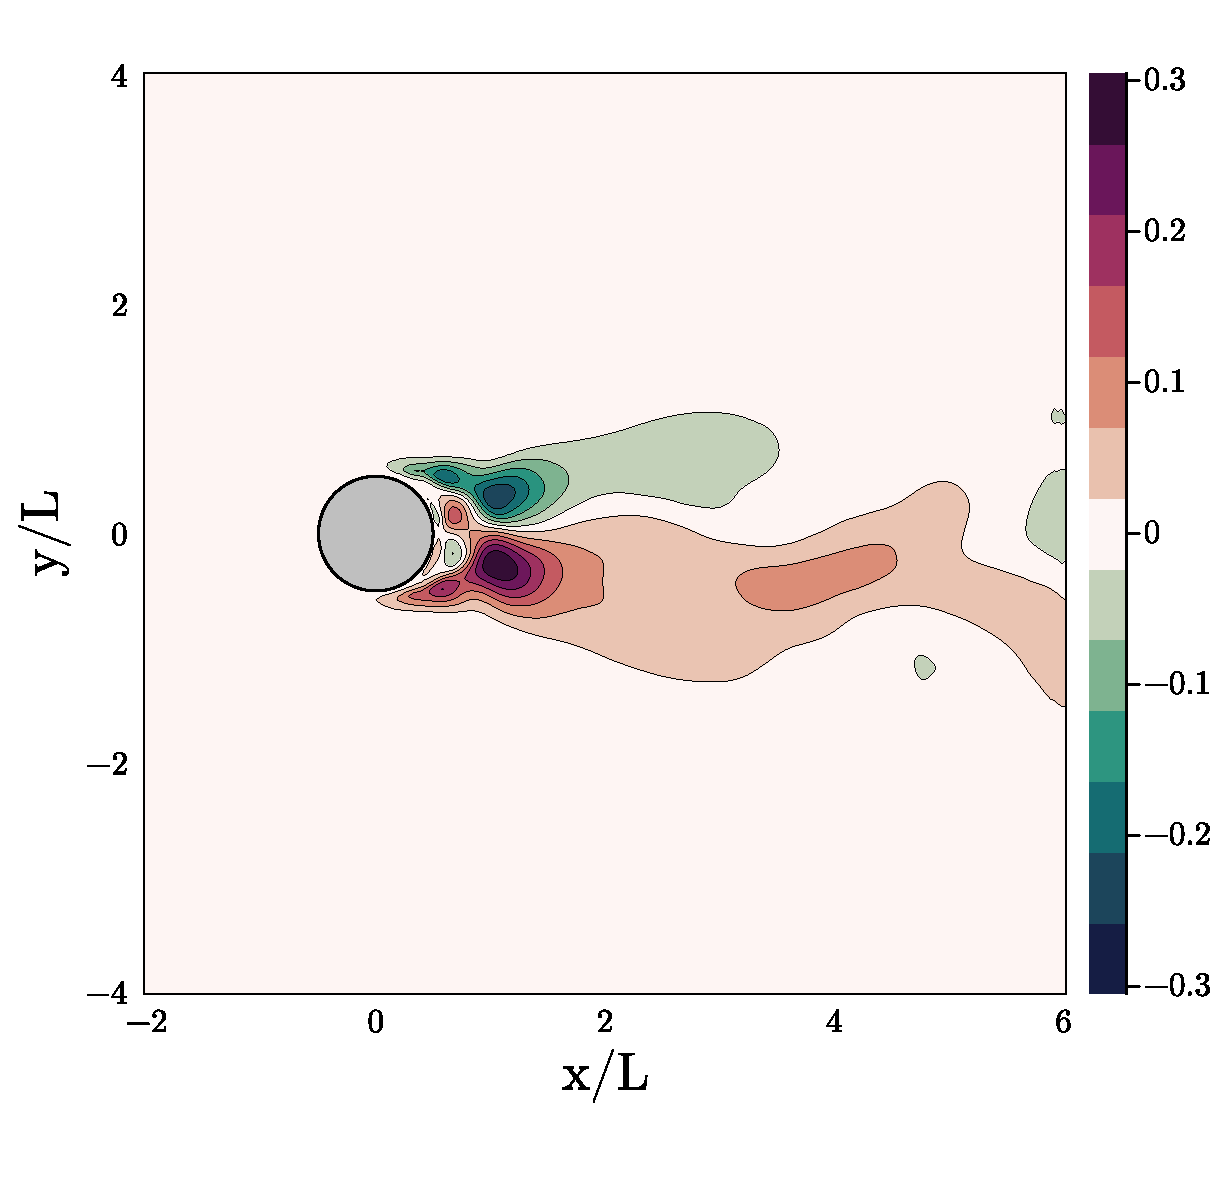
\includegraphics[width=\linewidth]{figures/Results/base/rst_panels/rst_uv_hybrid.pdf}
    % \caption{}
    \label{fig: base_rst_uv_hybrid}
  \end{subfigure}
  \begin{subfigure}[t]{0.3\textwidth}
    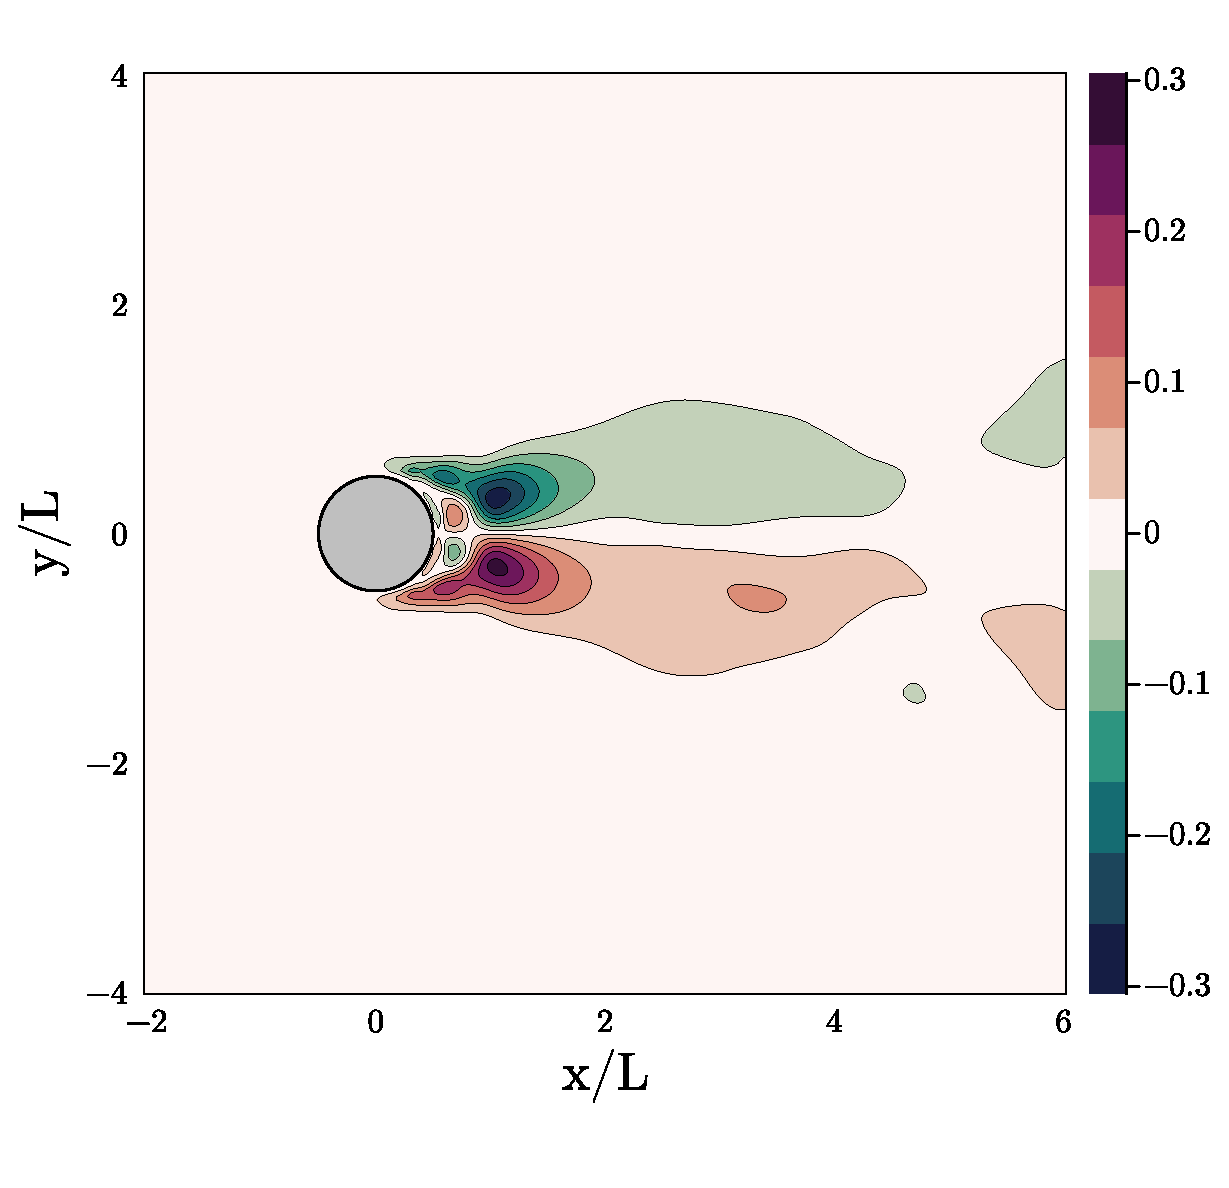
\includegraphics[width=\linewidth]{figures/Results/base/rst_panels/rst_uv_reference.pdf}
    % \caption{}
    \label{fig: base_rst_uv_ref}
  \end{subfigure}
  \begin{subfigure}[t]{0.3\textwidth}
    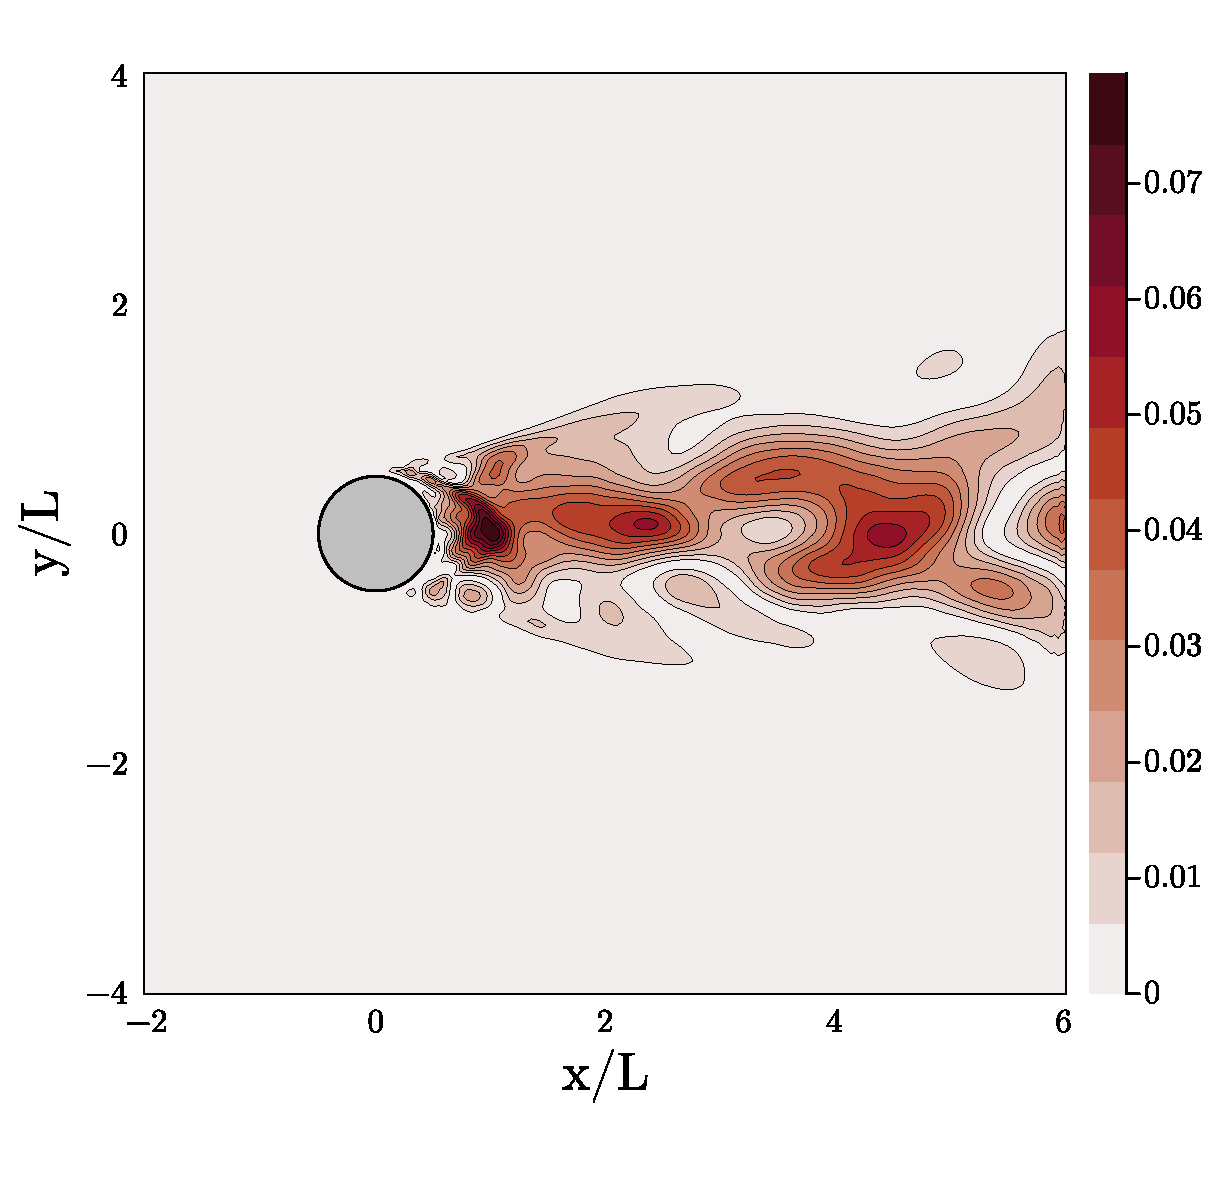
\includegraphics[width=\linewidth]{figures/Results/base/rst_panels/rst_uv_abserror.pdf}
    % \caption{}
    \label{fig: base_rst_uv_diff}
  \end{subfigure}
\vspace{-2em}
  \caption{Reynolds-stress components, top to bottom:
    $\langle u'u'\rangle$, $\langle v'v'\rangle$, $\langle u'v'\rangle$. Columns: hybrid $\mathcal{S}$, reference $\mathcal{S}_\text{ref}$, and absolute difference $\bigl|\mathcal{S}-\mathcal{S}_\text{ref}\bigr|$. Lengths scaled by $L$, velocities by $U$.}
  \label{fig: base_rst}
\end{figure}

Just as the RST components reported in the work by \textcite{Parnaudeau2008}, the hybrid and the reference simulation both produce the expected wake structure: a twin-lobed $\langle u'u'\rangle$ from the separating shear layers, a centreline-peaked $\langle v'v'\rangle$ in the region $1$--$2\, L$ downstream with the largest magnitude of the three, and an antisymmetric $\langle u'v'\rangle$ that vanishes on $y/L = 0$. The hybrid simulation closely recovers the normal stresses $\langle u'u'\rangle$ and $\langle v'v'\rangle$, matching both the peak locations and the lobe topology. The shear stress shows the biggest difference; the positive lobe is substantially weaker than in the reference, so the hybrid only partially preserves the antisymmetry over this simulation window.

The rightmost column of \autoref{fig: base_rst} shows the discrepancies, especially in the wake $x/L \gtrsim 1$, with peak errors of around $0.08$, $0.2$ and $0.08$ ($\sim\! 11, \; 16 \; \& \; 26 \%$ of the reference peaks); $\langle u'v'\rangle$ carries the largest relative error, as was also visible due to the fact that the positive half of its "butterfly" shape missing compared to the nicely symmetric contour plot of the reference shear component. Crucially, this error sits in the same near-body wake region as the mean-flow discrepancy (\autoref{fig: base_diff_mean_u}) and the rollout $4$--$6$ lift decay (\autoref{subsect: 4_forces}), which means that forces, mean flow, and Reynolds stresses indicate the same error for this hybrid case. As these figures have shown, however, the bias of $\mathcal{P}$ toward producing lower-amplitude fluctuations is an error in magnitude rather than a corruption of the dynamics. 

\begin{table}[htbp]
  \centering
  
  \begin{tabular}{l cc ccc}
    \toprule
    & \multicolumn{2}{c}{Mean flow} & \multicolumn{3}{c}{Reynolds stresses} \\
    \cmidrule(lr){2-3}\cmidrule(lr){4-6}
    & $\langle u\rangle$ & $\langle v\rangle$
    & $\langle u'u'\rangle$ & $\langle v'v'\rangle$ & $\langle u'v'\rangle$ \\
    \midrule
    $\varepsilon_q$  & 0.009 & 0.005 & 0.006 & 0.014 & 0.004  \\
    $\rho_q$        & 0.9932 & 0.9928 & 0.9789 & 0.9791 & 0.9275 \\
    \bottomrule
  \end{tabular}
    \caption{Quantitative comparison between the hybrid and reference fields: mean absolute error (MAE) and spatial Pearson correlation coefficient, computed over the wake region.}
    \label{tab: base_field_metrics}

\end{table}

While the contour plots in \autoref{fig: base_rst} convey the spatial agreement qualitatively, \autoref{tab: base_field_metrics} quantifies it for both the mean flow and the three RST components over the wake region. The mean flow is recovered almost exactly, with $\rho_q \approx 0.993$ for both $\langle u\rangle$ and $\langle v\rangle$. The normal stresses follow closely behind at $\rho_q \approx 0.979$, confirming that the hybrid field reproduces the wake topology correctly, just as was seen in the contours. The shear stress is the weakest component, dropping to $\rho_{u'v'} = 0.9275$; this lower value can be explained by the partially missing positive lobe; its small $\varepsilon_q = 0.004$ reflects the low magnitude of $\langle u'v'\rangle$ rather than close agreement. 

\subsection{Spectral Fidelity of the Wake}
\label{subsect: 4_physical_consistency}

In addition to the time-averaged statistics examined above, a physically faithful hybrid simulation must also reproduce the distribution of turbulent energy across temporal scales. This is assessed by sampling the transverse velocity $v$ at a fixed wake location $(x/L, y/L) = (2, 0.5)$ in both $\mathcal{S}$ and $\mathcal{S}_\text{ref}$. To separate the error introduced by the latent dynamics from that introduced by the autoencoder, a third signal is added: every snapshot of $\mathcal{S}_\text{ref}$ is passed through the trained autoencoder, $\hat{\mathbf{u}} = \psi_\theta(\varphi_\theta(\mathbf{u}))$, and the transverse velocity is extracted at the same downstream location. This per-frame reconstruction, labelled \emph{AE}, contains the reconstruction error of the decoder $\psi_\theta$ alone, with no contribution from the learned dynamics $f_\phi$, and therefore acts as a control that isolates the decoder's spectral signature.


The same three signals are shown in the time domain in \autoref{fig: base_vsignal}, together with the neural ODE rollout. The AE reconstruction tracks the reference closely but is slightly dissipative, smoothing the sharpest peaks and troughs of the velocity signal. The hybrid velocity signal, similar to the force coefficients in \autoref{fig: base_forces}, reproduces the shedding cycle but dampens its high-frequency oscillations relative to the reference and, in places, relaxes to a mean velocity signal rather than the full fluctuations, most visibly in the second hybrid region.


\begin{figure}[htbp]
    \centering
    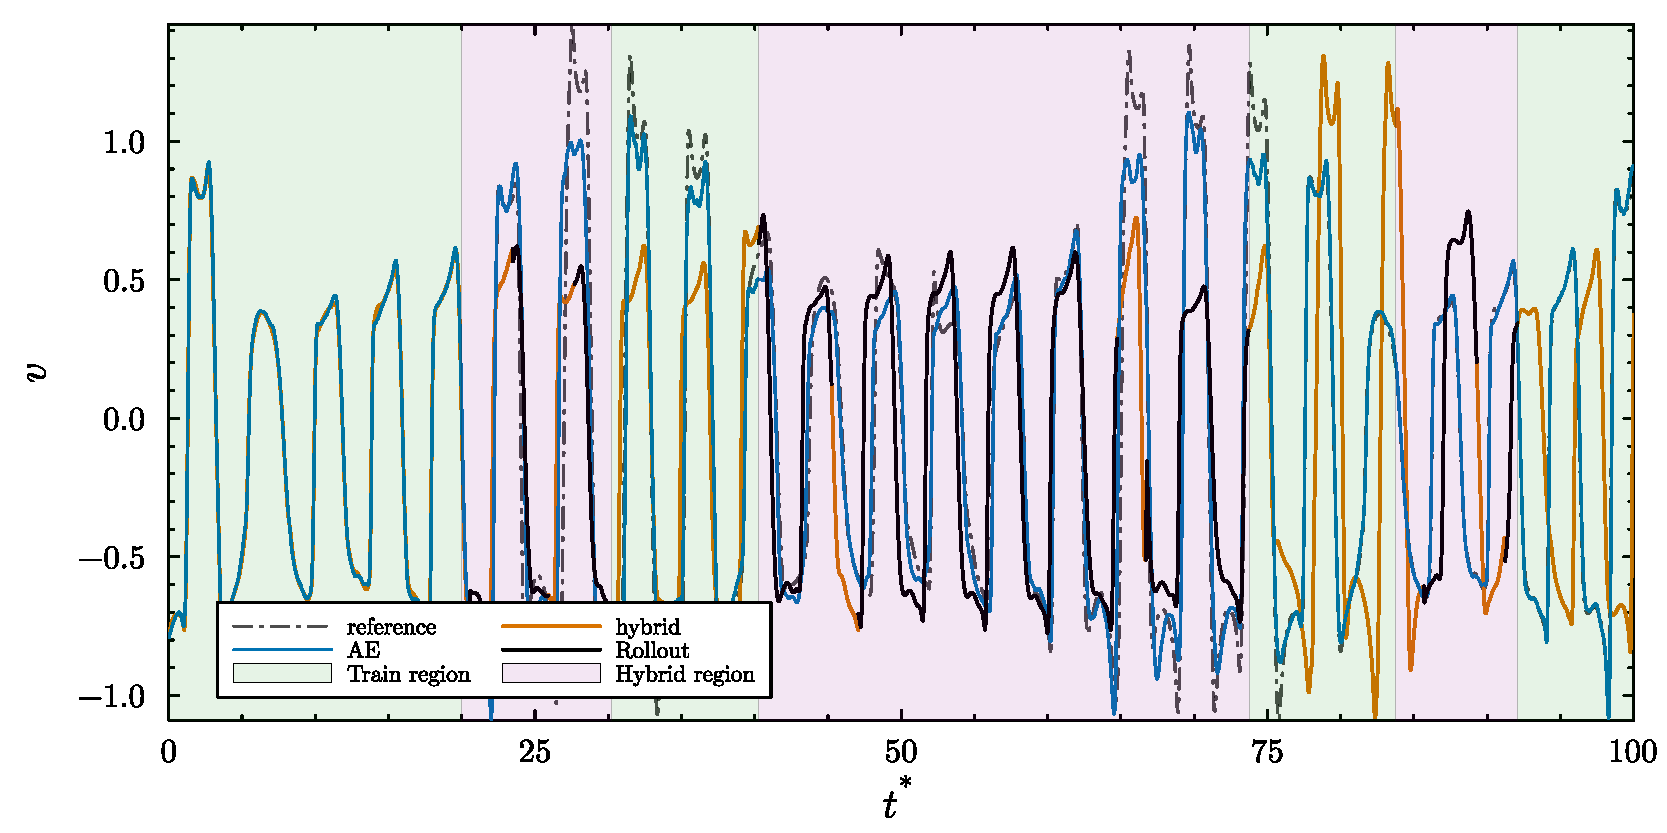
\includegraphics[width=\linewidth]{figures/Results/base/wake_signal.pdf}
    \caption{Transverse wake velocity $v$ at the probe $(x/L, y/L) = (2, 0.5)$ against non-dimensional time $t^*$, for the reference, the per-frame AE reconstruction, the hybrid simulation. Shaded bands mark the training and hybrid windows.}
    \label{fig: base_vsignal}
\end{figure}

These signals are compared in the frequency domain via their one-sided power spectra $\mathrm{PS}(v)$, estimated using Welch's method with five segments of the simulation window. Each segment, therefore, spans approximately five shedding periods. The resulting spectra are shown in \autoref{fig: base_psd} against the non-dimensional frequency $fL/U$.

In the low-frequency part of the spectrum, all three signals produce the same frequencies. The primary shedding frequency is clearly present at $fL/U \approx 0.2$ in every case, as was already visible in the force coefficient plot in \autoref{fig: base_forces}; the higher harmonics of the shedding frequency, associated with the secondary wake structures displayed in \autoref{fig: vortex_shedding}, are also captured by both the hybrid simulation and the AE reconstruction. The hybrid, AE and reference curves remain closely aligned through the middle frequency range, until they separate near $fL/U \approx 2$--$3$. No genuine Kolmogorov $f^{-5/3}$ inertial subrange is expected in a two-dimensional wake at $Re=2500$; in two dimensions the forward (small-scale) cascade follows the steeper $k^{-3}$ enstrophy scaling rather than $k^{-5/3}$ \cite{Boffetta2011}, which under Taylor's frozen-turbulence hypothesis maps to the $f^{-3}$ reference slope shown in \autoref{fig: base_psd}.

\begin{figure}[htbp]
    \centering
    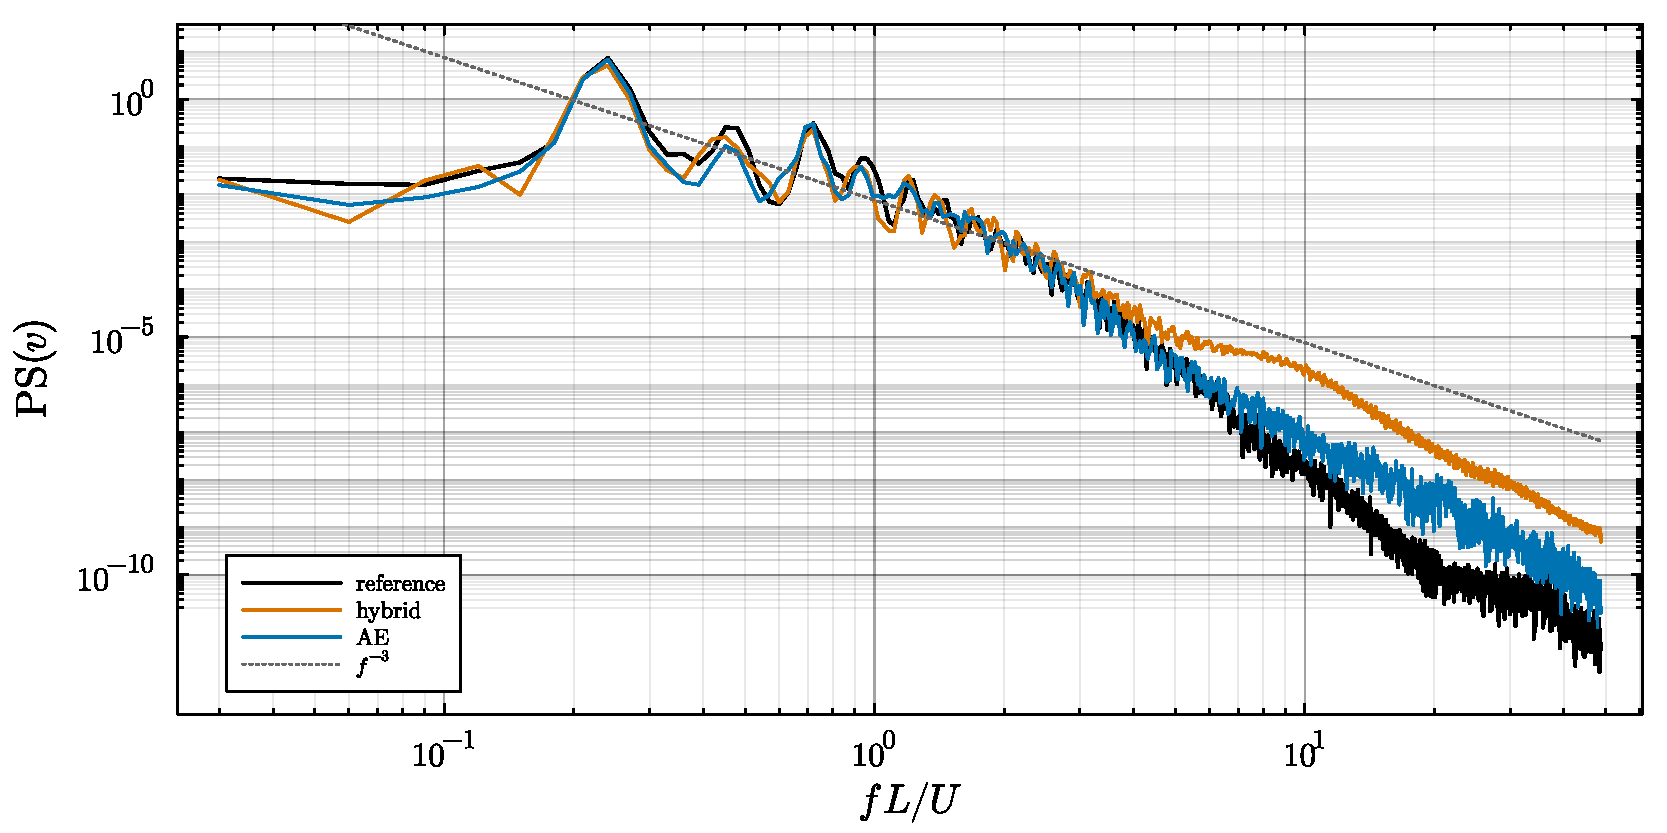
\includegraphics[width=\linewidth]{figures/Results/base/wake_psd.pdf}
    \caption{Power spectrum of the transverse wake velocity $\mathrm{PS}(v)$ for the reference $\mathcal{S}_\text{ref}$, the hybrid $\mathcal{S}$, and the per-frame autoencoder reconstruction of $\mathcal{S}_\text{ref}$ (AE), against the non-dimensional frequency $fL/U$. The dotted line marks an $f^{-3}$ slope, shown only as a visual reference for the 2D mid-band decay rate.}  
    \label{fig: base_psd}
  \end{figure}


Beyond the crossover near $fL/U \approx 2$--$4$, the three spectra spread out into a clear ordering: the reference falls steeply to $\mathcal{O}(10^{-10})$, the AE reconstruction plateaus roughly two to three decades above it, and the hybrid plateaus a further decade above the AE. This ordering shows how the errors are stacked in $\mathcal{P}$, with the AE spectrum being the lower bound for error for the hybrid simulation, as all snapshots produced by $\mathcal{P}$ must pass through it. It lies above the reference spectrum because the reconstruction error of $\psi_\theta$ adds a high-wavenumber texture from the bilinear-upsampling decoder, which only gets visible when the true spectrum $\mathrm{PS}(v)$ has fallen below it.

When looking at the spectrum of the hybrid simulation, it sits elevated above the AE spectrum, indicating that the higher-frequency energy cannot be a decoder effect, since both fields are reconstructed using the same $\psi_\theta$; instead, it is a property of the neural ODE rollouts and their coupling to WaterLily. Two mechanisms contribute to this added error: first, the AE reconstructs instantaneous latents encoded from true reference fields, whereas the hybrid decodes latent vectors integrated by $f_\phi$, which exhibit a degree of drift relative to the ground truth. Because the decoder maps a $16$-dimensional latent onto a $256 \times 256$ field, it can be locally sensitive, so that a small drift $\delta\mathbf{z}$ in the latent state is amplified into a comparatively large perturbation in physical space. Secondly, the hybrid signal is a concatenation of latent-rollout and WaterLily segments spliced at every OOD fallback, so each re-injected field and the solver's relaxation of it can introduce a discontinuity in $v$, visible as a kink in the hybrid trace in \autoref{fig: base_vsignal}. Each such discontinuity adds energy at high frequencies, lifting the tail above the reference and the AE signal and flattening its decay during the $fL/U \approx 5$--$10$  frequency band; the tail still falls off at high $fL/U$ and follows the same slope as the reference.

Despite the elevated tail of the hybrid spectrum, the added high-frequency energy remains low in absolute terms. Since it lies more than 2 decades below the shedding frequency, it would contribute negligibly to the integrated signal energy. The dominant scales, namely the primary shedding frequency and its harmonics, are reproduced accurately by both the AE reconstruction and the hybrid simulation. The spectral discrepancy is therefore confined to a low-energy, high-frequency band where the true spectrum has already decayed, and does not compromise the physical fidelity of the resolved flow. The concentration of error in the high-frequency, low-energy range, where the true signal is weakest, is a recurring difficulty for learned models advanced autoregressively over long horizons \cite{Lippe2023}.


\subsection{Autoencoder performance}
\label{subsect: 4_ae_performance}

The autoencoder is the entry and exit point of every $\tilde{\boldsymbol{\mathcal{T}}}_z$ because every initial state is first compressed by $\varphi_\theta$, and every field returned to $\mathcal{S}$ is reconstructed by $\psi_\theta$. Its round-trip error \eqref{eq: AE_loss} therefore sets a lower bound on the maximal accuracy $\mathcal{P}$ can attain, independent of how well the latent dynamics can be predicted. Understanding how the autoencoder performs is therefore crucial for interpreting the baseline results of \autoref{subsect: 4_forces}, since any error already present in the reconstruction cannot be attributed to $f_\phi$. 

\subsubsection{Training dynamics}

\begin{figure}[htp]
    \centering
    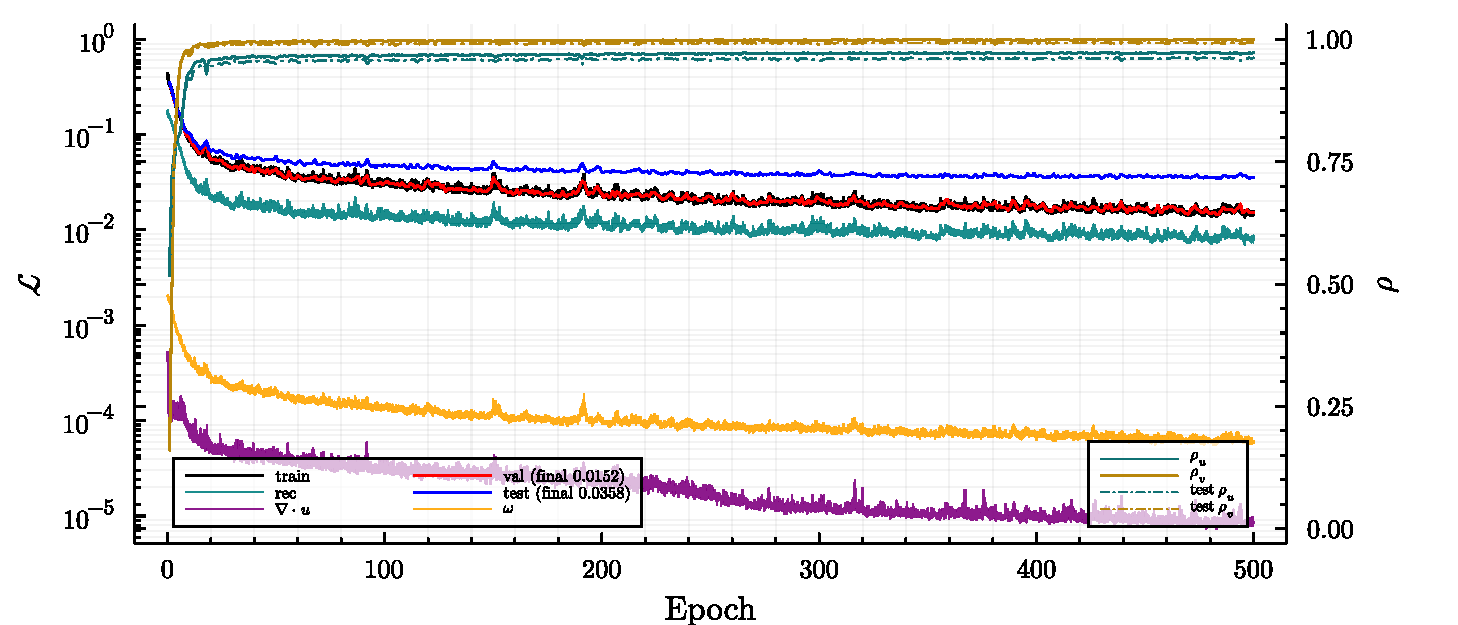
\includegraphics[width=\linewidth]{figures/Results/base/loss_evolution.pdf}
    \caption{Initial training history of the baseline autoencoder. Left axis ($\mathcal{L}$, logarithmic): the total loss on the train, validation and test splits, together with the divergence ($\nabla\!\cdot\mathbf{u}$) and vorticity ($\omega$) penalty terms evaluated on the test split. Right axis ($\rho$): the reconstruction correlation coefficients $\rho_u$ and $\rho_v$ on train and test.}
    \label{fig: initial_training_base}
\end{figure}

\autoref{fig: initial_training_base} shows the loss history of the initial autoencoder training, using the parameters listed in \autoref{tab: 4_ae_config}, on the initial data-gathering trajectory sampled up to $t^*_\text{train}=17.5$. The reconstruction loss on the train and validation splits converge to $\mathcal{L}\approx1.5\times10^{-2}$, while the divergence and vorticity penalties settle near $10^{-5}$ and $10^{-4}$ respectively. The correlation coefficients of both velocity components also quickly approach unity, indicating that flow structure is learned rapidly. The test loss settles at $3.55\times10^{-2}$, which is about twice the validation loss value; this value is determined on the held-out window $t^*\in[17.5,\,20]$. This gap indicates that the initial training window lacked sufficient information about the spatial dynamics of $\mathcal{S}$, suggesting that more data are required for generalisation across the entire simulation window, motivating the need to update the autoencoder weights $\theta$. 

\begin{figure}[htp]
    \centering
    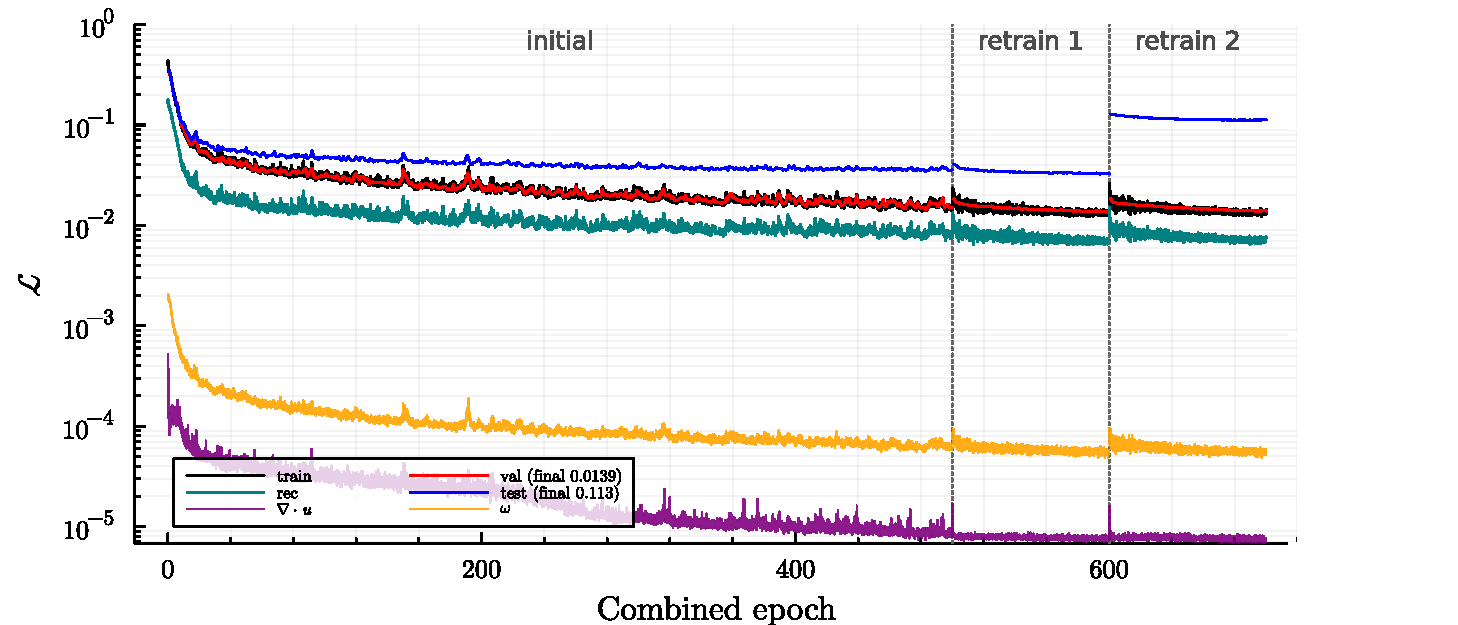
\includegraphics[width=\linewidth]{figures/Results/base/combined_loss_evolution.pdf}
    \caption{Combined training history of the baseline autoencoders. Left axis ($\mathcal{L}$, logarithmic): Showing how the cost function of the autoencoder varies over retraining runs, indicating the correlation of the training set to the current simulation state.}
    \label{fig: combined_training_base}
\end{figure}

\autoref{fig: combined_training_base} extends the loss over the 2 retraining stages, where each stage updates the weights for an additional $100$ epochs using a reduced learning rate (\autoref{subsect: retraining}). The first learning rate leaves the losses mostly unchanged, but with additional data, it has learned additional dynamics, reflected in the ability to perform longer rollouts, as discussed in \autoref{subsect: 4_forces}. The second retrain drives the test loss up by nearly an order of magnitude while train and validation hold steady: the accumulated dissipative drift (\autoref{subsect: 4_forces}) has pushed $\mathcal{S}$ into a regime that is under-represented in the training data, which makes it so that the generalisation outside of the training regime drastically worsens. This same disparity in training data, and current state of $\mathcal{S}$, is also reflected in the immediately truncated rollouts $7$ and $9$ (\autoref{tab: base_rollout_summary}).

\subsubsection{Instantaneous reconstruction performance}
The reconstruction of an instantaneous velocity field is displayed in  \autoref{fig: base_velocity_comp} for the two velocity components. These figures show that $\psi_\theta$ performs well in reconstructing the large scale structures of the flow, aligning with the conclusions from \autoref{subsect: 4_physical_consistency}.

\begin{figure}[htp]
    \centering
    \begin{tikzpicture}
        \node[anchor=south west, inner sep=0] (img)
            {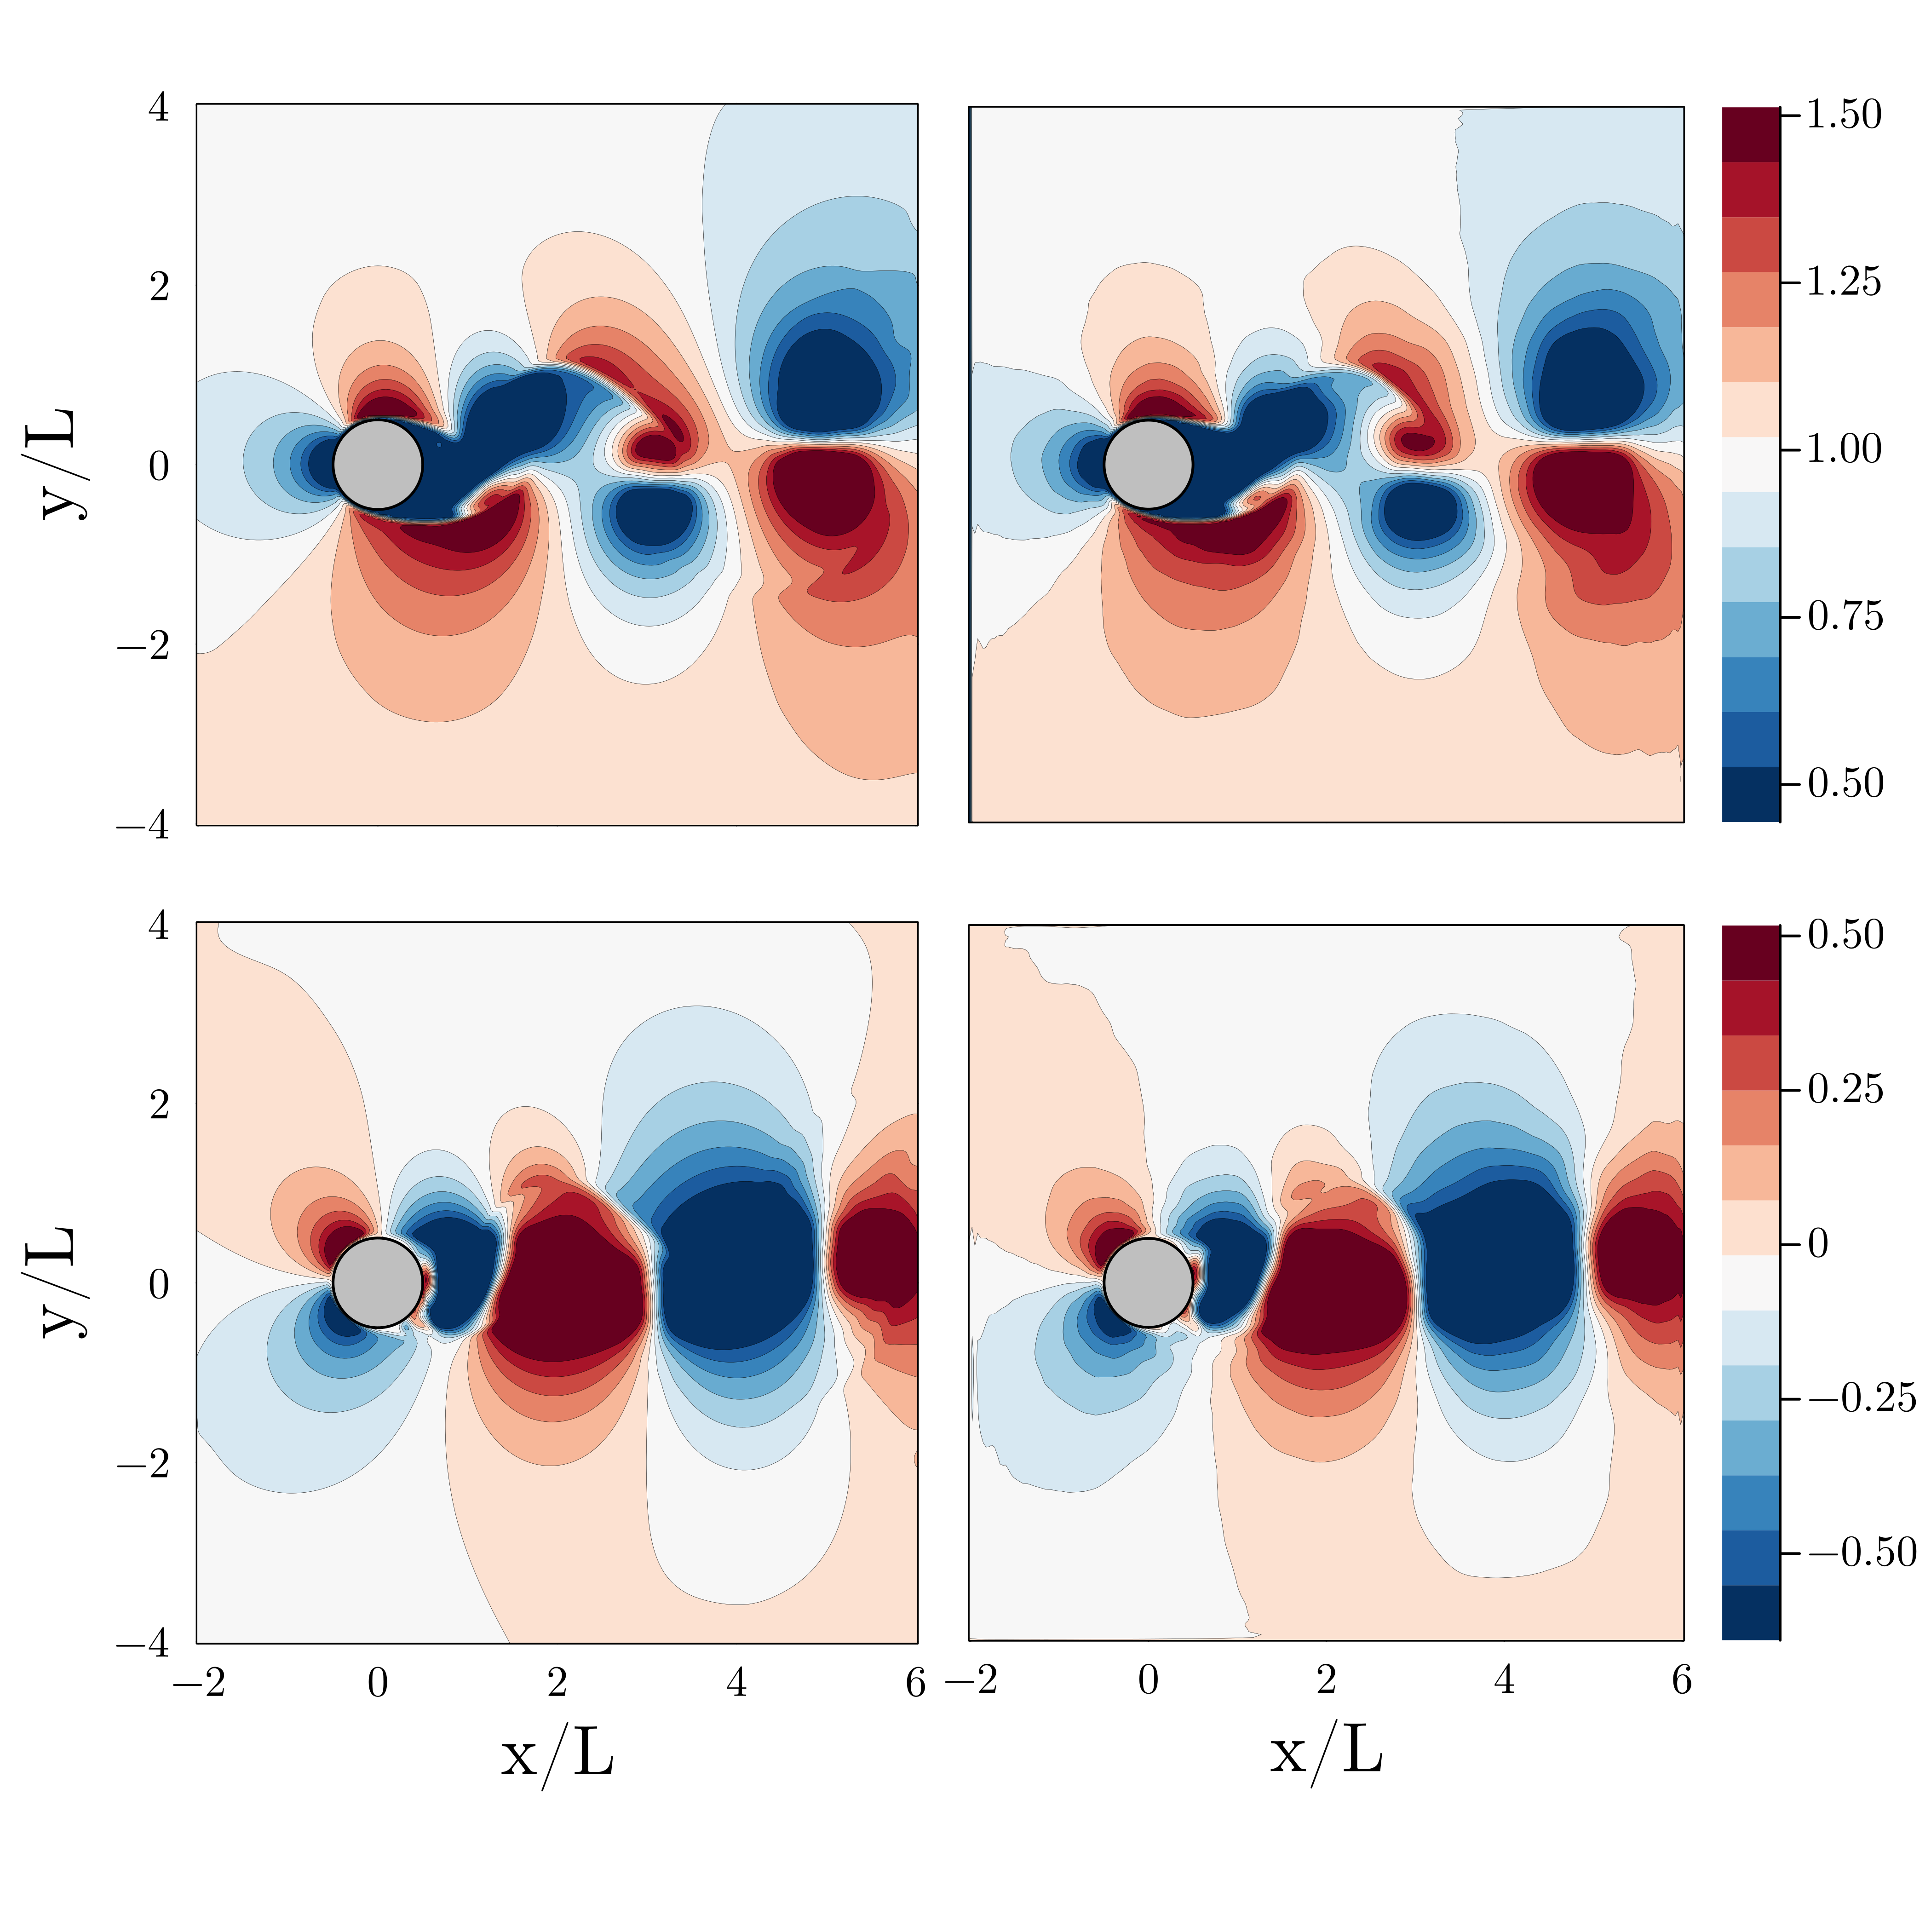
\includegraphics[width=0.9\linewidth]{figures/Results/base/velocity_comp.png}};
        % normalised coords: (0,0)=bottom-left, (1,1)=top-right of the image
        \begin{scope}[x={(img.south east)}, y={(img.north west)}]
            % --- column headers ---
            \node[anchor=south] at (0.30, 0.95) {\large $\mathbf{u}$};
            \node[anchor=south] at (0.7, 0.95) {\large $\hat{\mathbf{u}}$};
            % --- row labels ---
            % \node[rotate=90, anchor=center] at (-0.02, 0.75) {$u/U$};
            % \node[rotate=90, anchor=center] at (-0.02, 0.3) {$v/U$};
        \end{scope}
    \end{tikzpicture}
    \vspace{-2em}
    \caption{Instantaneous reconstruction of the velocity field by the baseline autoencoder at $t^*=40.46$. Top row: streamwise component $u$; bottom row: transverse component $v$. Left column: WaterLily reference; right column: instantaneous autoencoder reconstruction $\hat{\mathbf{u}}=\psi_\theta(\varphi_\theta(\mathbf{u}))$}
    \label{fig: base_velocity_comp}
\end{figure}

The instantaneous reconstructions are visibly smoother than the reference, most notably along the thin shear layers separating from the cylinder. These over-smoothing and the concentration of error in high-gradient regions are documented failure modes of autoencoders applied to turbulent flows, as they have shown to reproduce the large-scale coherent structures correctly but act as nonlinear filters that attenuate the small-scale, high-wavenumber content~\cite{Lu2025, Glaws2020, Jeon2022}. These smoother gradients, especially at the cylinder wall, are the direct explanation of the dissipative bias seen in the integrated forces, since the structures re-injected into $\mathcal{S}$ are systematically weaker than the reference.

This "smoothing" of the reconstructed field is more apparent when computing the vorticity using the reconstructed velocity components. The instantaneous vorticity in \autoref{fig: base_curl_comp} shows how the effect of the more smeared out velocity gradients.

\begin{figure}[htp]
    \centering
    \begin{tikzpicture}
        \node[anchor=south west, inner sep=0] (img)
            {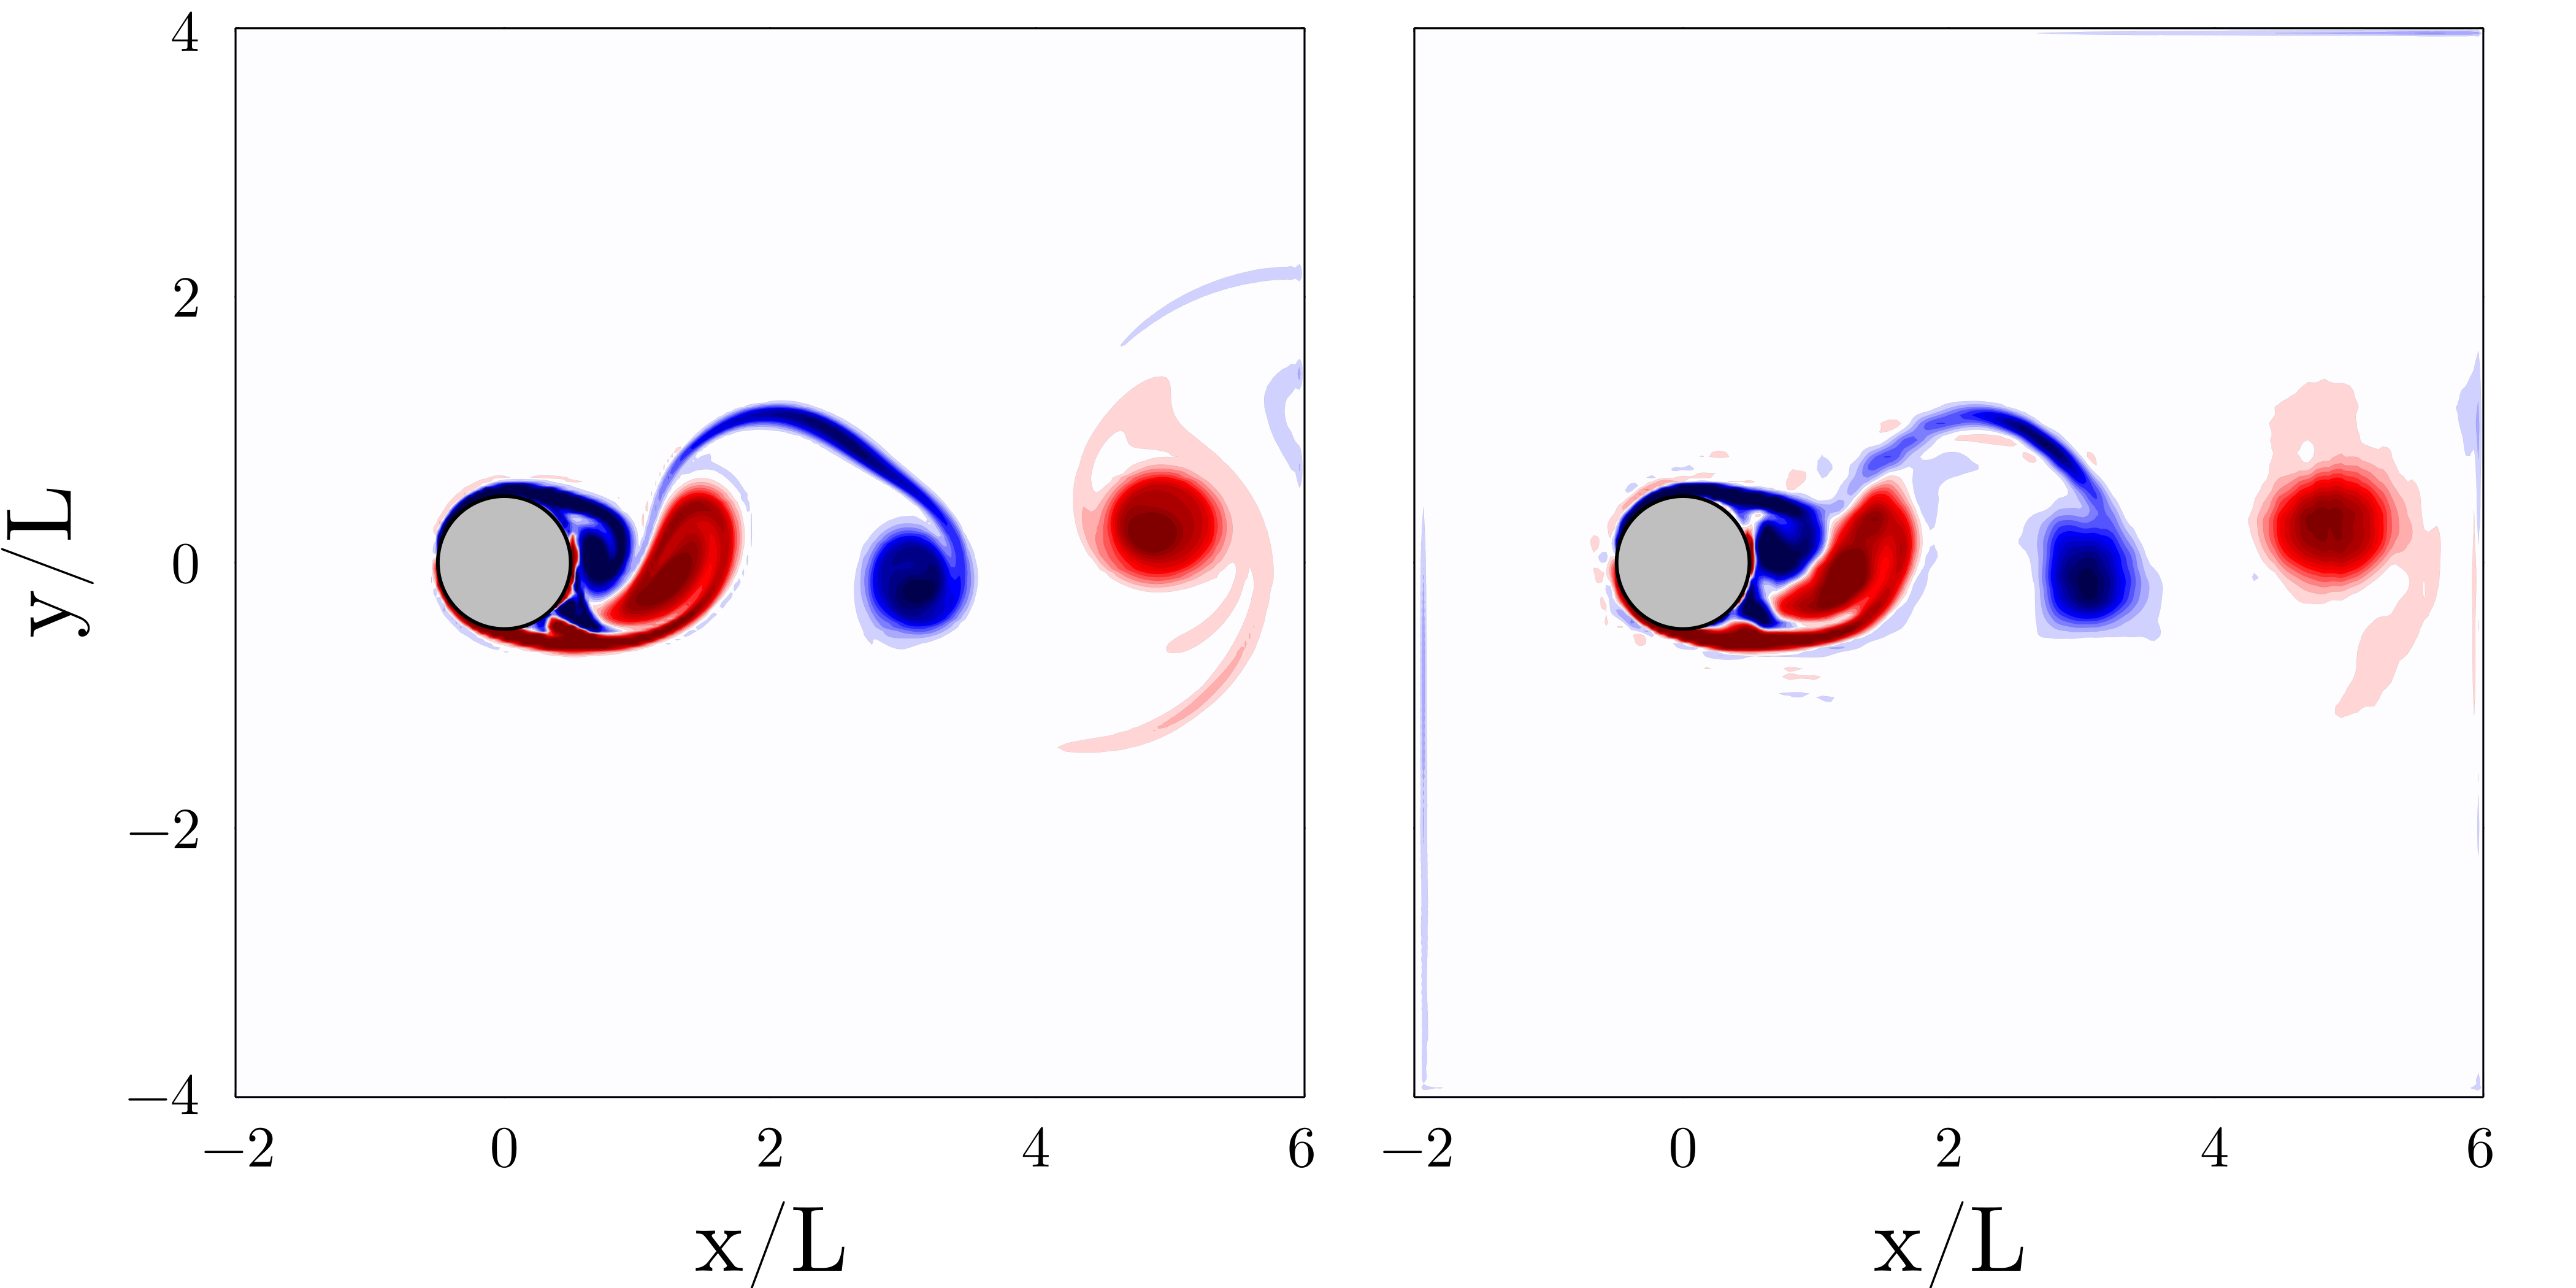
\includegraphics[width=.95\linewidth]{figures/Results/base/curl_comp.png}};
        % normalised coords: (0,0)=bottom-left, (1,1)=top-right of the image
        \begin{scope}[x={(img.south east)}, y={(img.north west)}]
            % --- column headers ---
            \node[anchor=south] at (0.275, 0.95) {Reference};
            \node[anchor=south] at (0.675, 0.95) {Reconstructed};
            % --- row labels ---
            % \node[rotate=90, anchor=center] at (-0.02, 0.75) {$u/U$};
            % \node[rotate=90, anchor=center] at (-0.02, 0.3) {$v/U$};
        \end{scope}
    \end{tikzpicture}
 \caption{Instantaneous vorticity $\omega$ of the same snapshot as \autoref{fig: base_velocity_comp}. Left: WaterLily reference; right: autoencoder reconstruction. The reconstructed shear layers and vortex cores are diffused and exhibit reduced peak amplitudes, illustrating the autoencoder's low-pass behaviour.}
    \label{fig: base_curl_comp}
\end{figure}

The reference shear layers and shed vortex cores are sharp and compact, whereas the reconstructed field is diffuse: the cores are spread over a wider area at reduced peak amplitude, and the thin braid of vorticity in the immediate wake is largely smeared out. \autoref{fig: base_curl_comp} also shows the addition of noisy artefacts in the near-wall region and close to the vortices, which explains the presence of the added noise observed in \autoref{subsect: 4_physical_consistency}. A further band of spurious vorticity is also visible along the reconstructed domain boundary in \autoref{fig: base_curl_comp}; this is not physical but a boundary artefact of the convolutional decoder, where the zero-padding biases the outermost cells and this small velocity deviation is amplified by the gradient operator used to compute $\omega = \hat{u}_{2,1} - \hat{u}_{1,2}$. This deviation generally stays confined to the outer edge of the domain and has no effect on the wake and near-body forces and metrics reported in this section


Overall, the autoencoder faithfully reproduces the large-scale structures in the wake and shedding cycle, with $\rho_u,\, \rho_v$ converging near unity, at the cost of attenuating the small-scale content revealed by the vorticity field. These characteristics set the pipeline's accuracy floor; investigating whether it can be lowered by varying the latent dimension, or the training procedures, is the subject of the parameter study in \autoref{subsect: 4_ae_parameters}.


\subsection{NODE performance}
\label{subsect: 4_node_performance}

With the autoencoder's performance over the hybrid simulation characterised and the spatial accuracy floor thereby fixed, the learning behaviour of $f_\phi$ can now be traced through the simulation to understand the neural ODE's inference behaviour. The latent dynamics are followed from the initial multiple-shooting fit through to the retraining optimisations that the hybrid loop relies on, tracking how their fidelity evolves as $f_\phi$ is retrained on the growing set of trajectories.

\autoref{fig: base_node_ms} shows the initial multiple-shooting training. Within every segment, the prediction $\tilde{z}$ tracks the reference $z$ closely, and the shooting gaps at the segment boundaries have closed to the point of being barely visible. The fit is visibly converged, but it is also segment-wise: the loss~\eqref{eq: node_loss_ms} only ever penalises $f_\phi$ over a single span of $n_s$ samples at a time. The training scheme, therefore, biases $f_\phi$ towards short-horizon accuracy and reveals nothing about how the dynamics compound once the segment resets are removed.

\begin{figure}[htbp]
    \centering
    \begin{subfigure}[t]{0.48\textwidth}
        \centering
        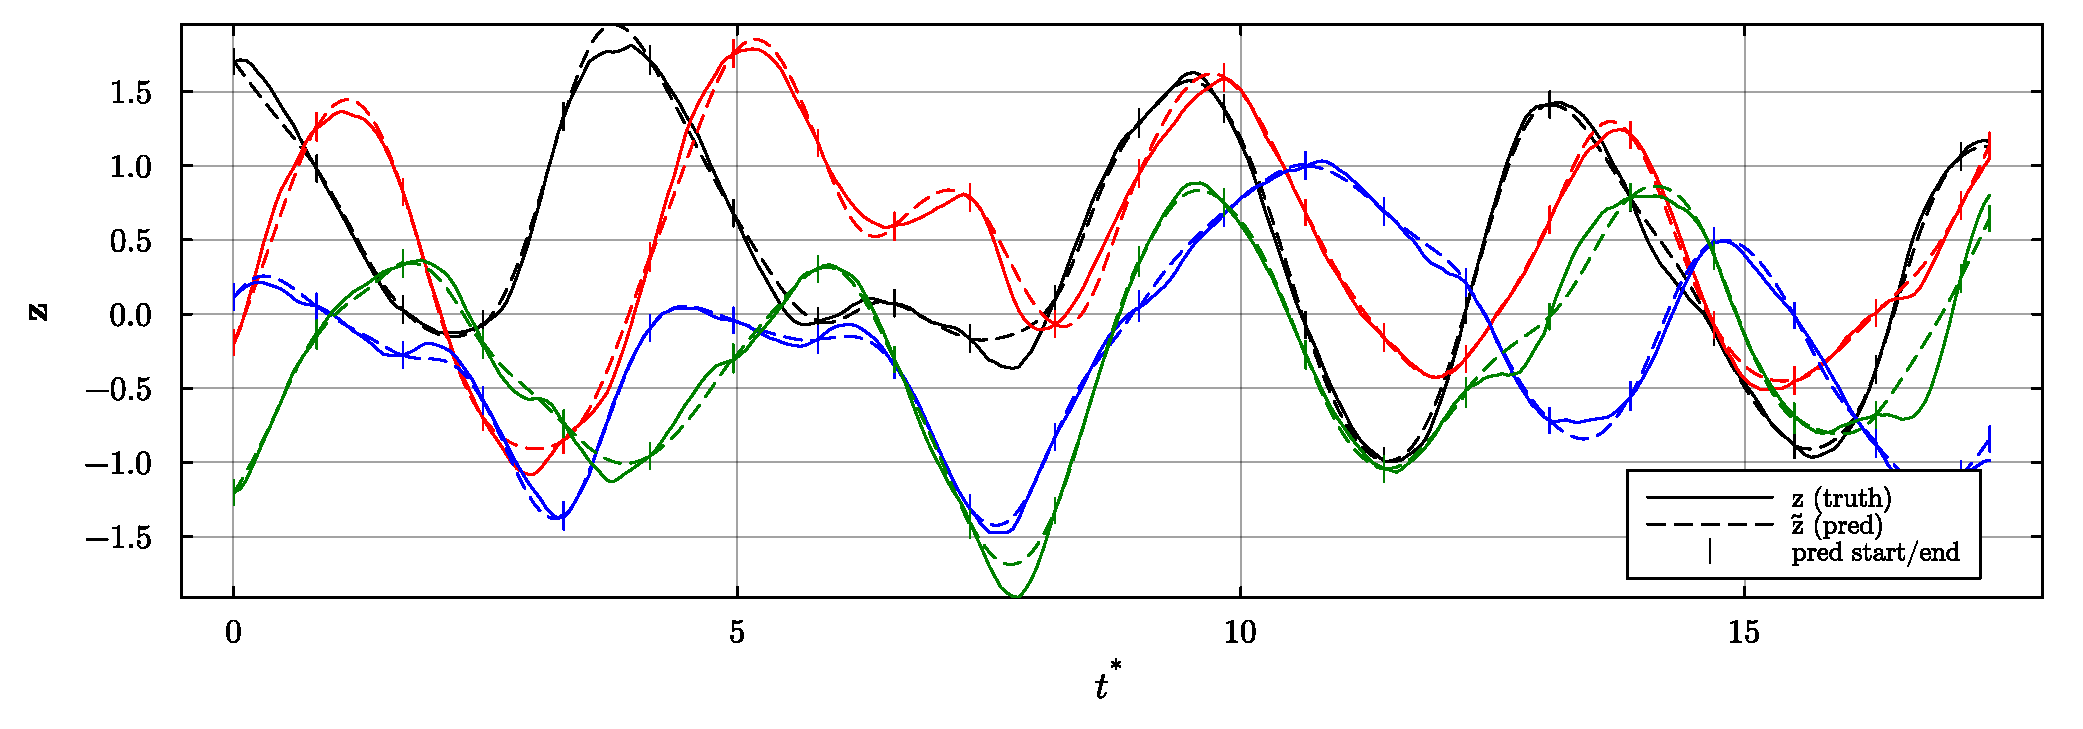
\includegraphics[width=\linewidth]{figures/Results/base/trajectories.pdf}
    \caption{Converged multiple-shooting fit; markers denote the start and end of each shooting segment.}
    \label{fig: base_node_ms}
    \end{subfigure}
    \hfill
    \begin{subfigure}[t]{0.48\textwidth}
        \centering
        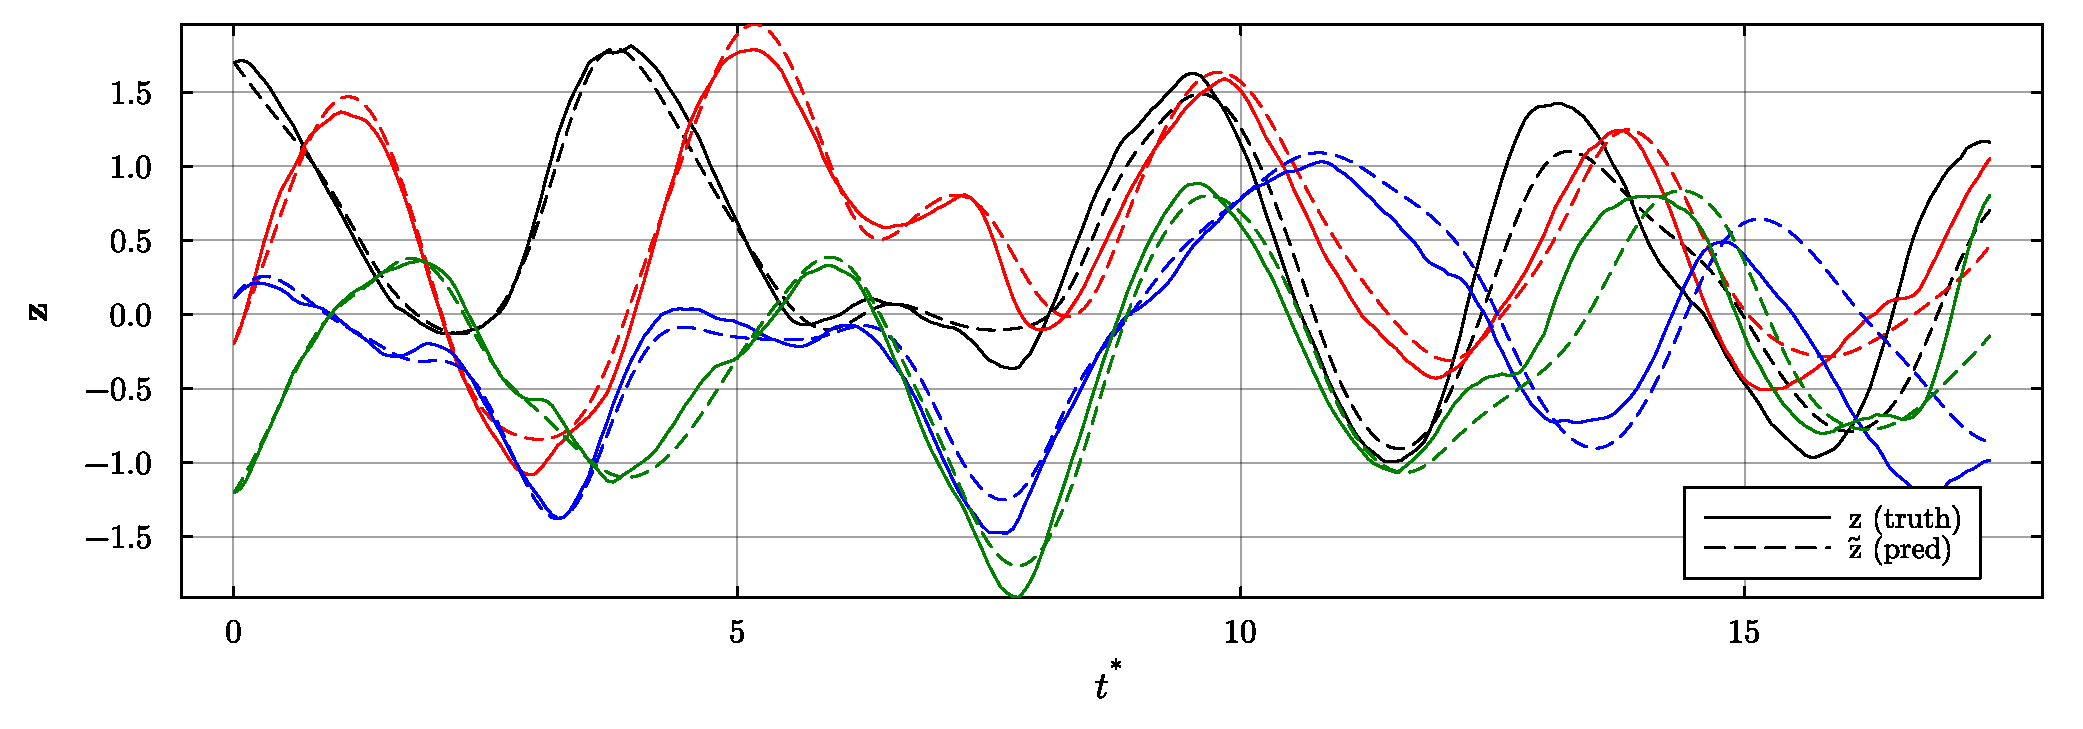
\includegraphics[width=\linewidth]{figures/Results/base/rollout_single_shooting.pdf}
        \caption{Single rollout from $t^*=0$ over the full training span, no segment resets.}
        \label{fig: base_node_singleshoot}
    \end{subfigure}
    \caption{Latent dynamics of the baseline $f_\phi$ over the initial training span, four representative components shown. Reference $z$ (solid) against prediction $\tilde{z}$ (dashed). (a) Converged multiple-shooting fit, with segment start/end markers; (b) unaided single rollout integrated from $t^*=0$ over the same window.}
\label{fig: base_node_rollout}
\end{figure}

The compounding error over longer rollouts is exposed in \autoref{fig: base_node_singleshoot}, where $f_\phi$ is integrated from $t^*=0$ over the whole span. The dominant shedding oscillation is recovered correctly: phase and amplitude of the leading components track the reference through the first several periods, confirming that $f_\phi$ has learned the principal latent dynamics rather than merely interpolating between segment endpoints. Towards the end of the window, however, a clear mismatch is evident, with both a phase and an amplitude deficit relative to $z$. The long rollout thus sustains the correct dynamics over a limited horizon before drifting, which gets controlled by the KNN monitor. 

After this first fit has concluded, the hybrid loop is ready to begin rolling out and accelerating the simulation; once the monitor has raised $n_\text{max, flags}$ flags, retraining is triggered, and $f_\phi$ is refitted on the augmented trajectory set $\boldsymbol{\mathcal{T}}_z^{(r+1)}$.

\begin{figure}[htbp]
    \centering
    \begin{subfigure}[t]{0.48\textwidth}
        \centering
        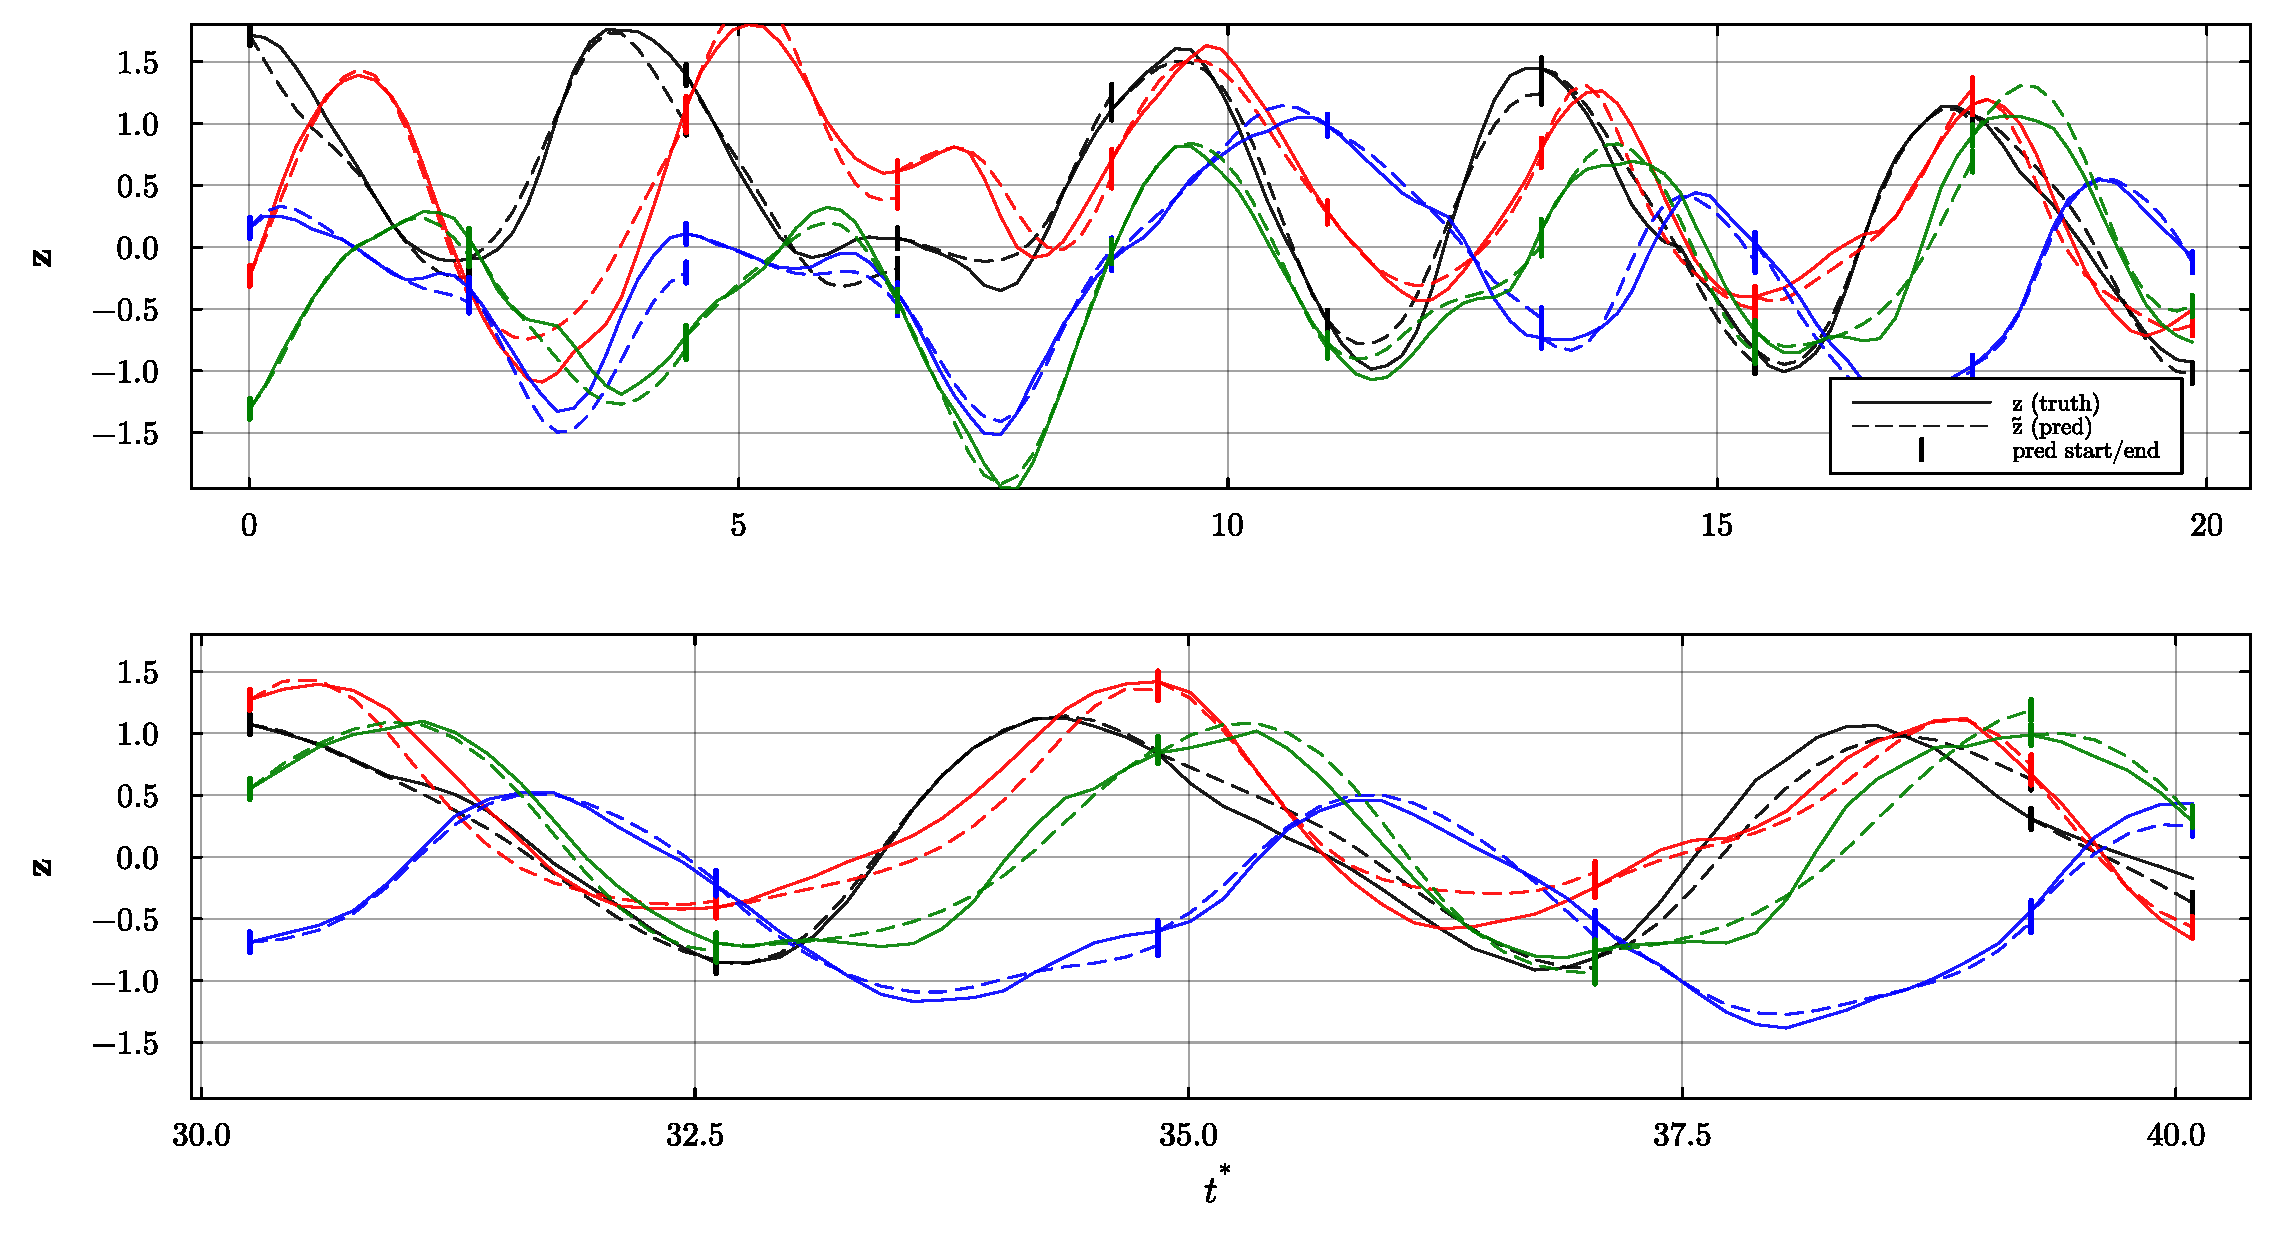
\includegraphics[width=\linewidth]{figures/Results/base/multiple_shoot_multi.pdf}
    \caption{Converged multiple-shooting fit on the augmented trajectory set; markers denote shooting-segment boundaries.}
    \label{fig: retrain_node_ms}
    \end{subfigure}
    \hfill
    \begin{subfigure}[t]{0.48\textwidth}
        \centering
        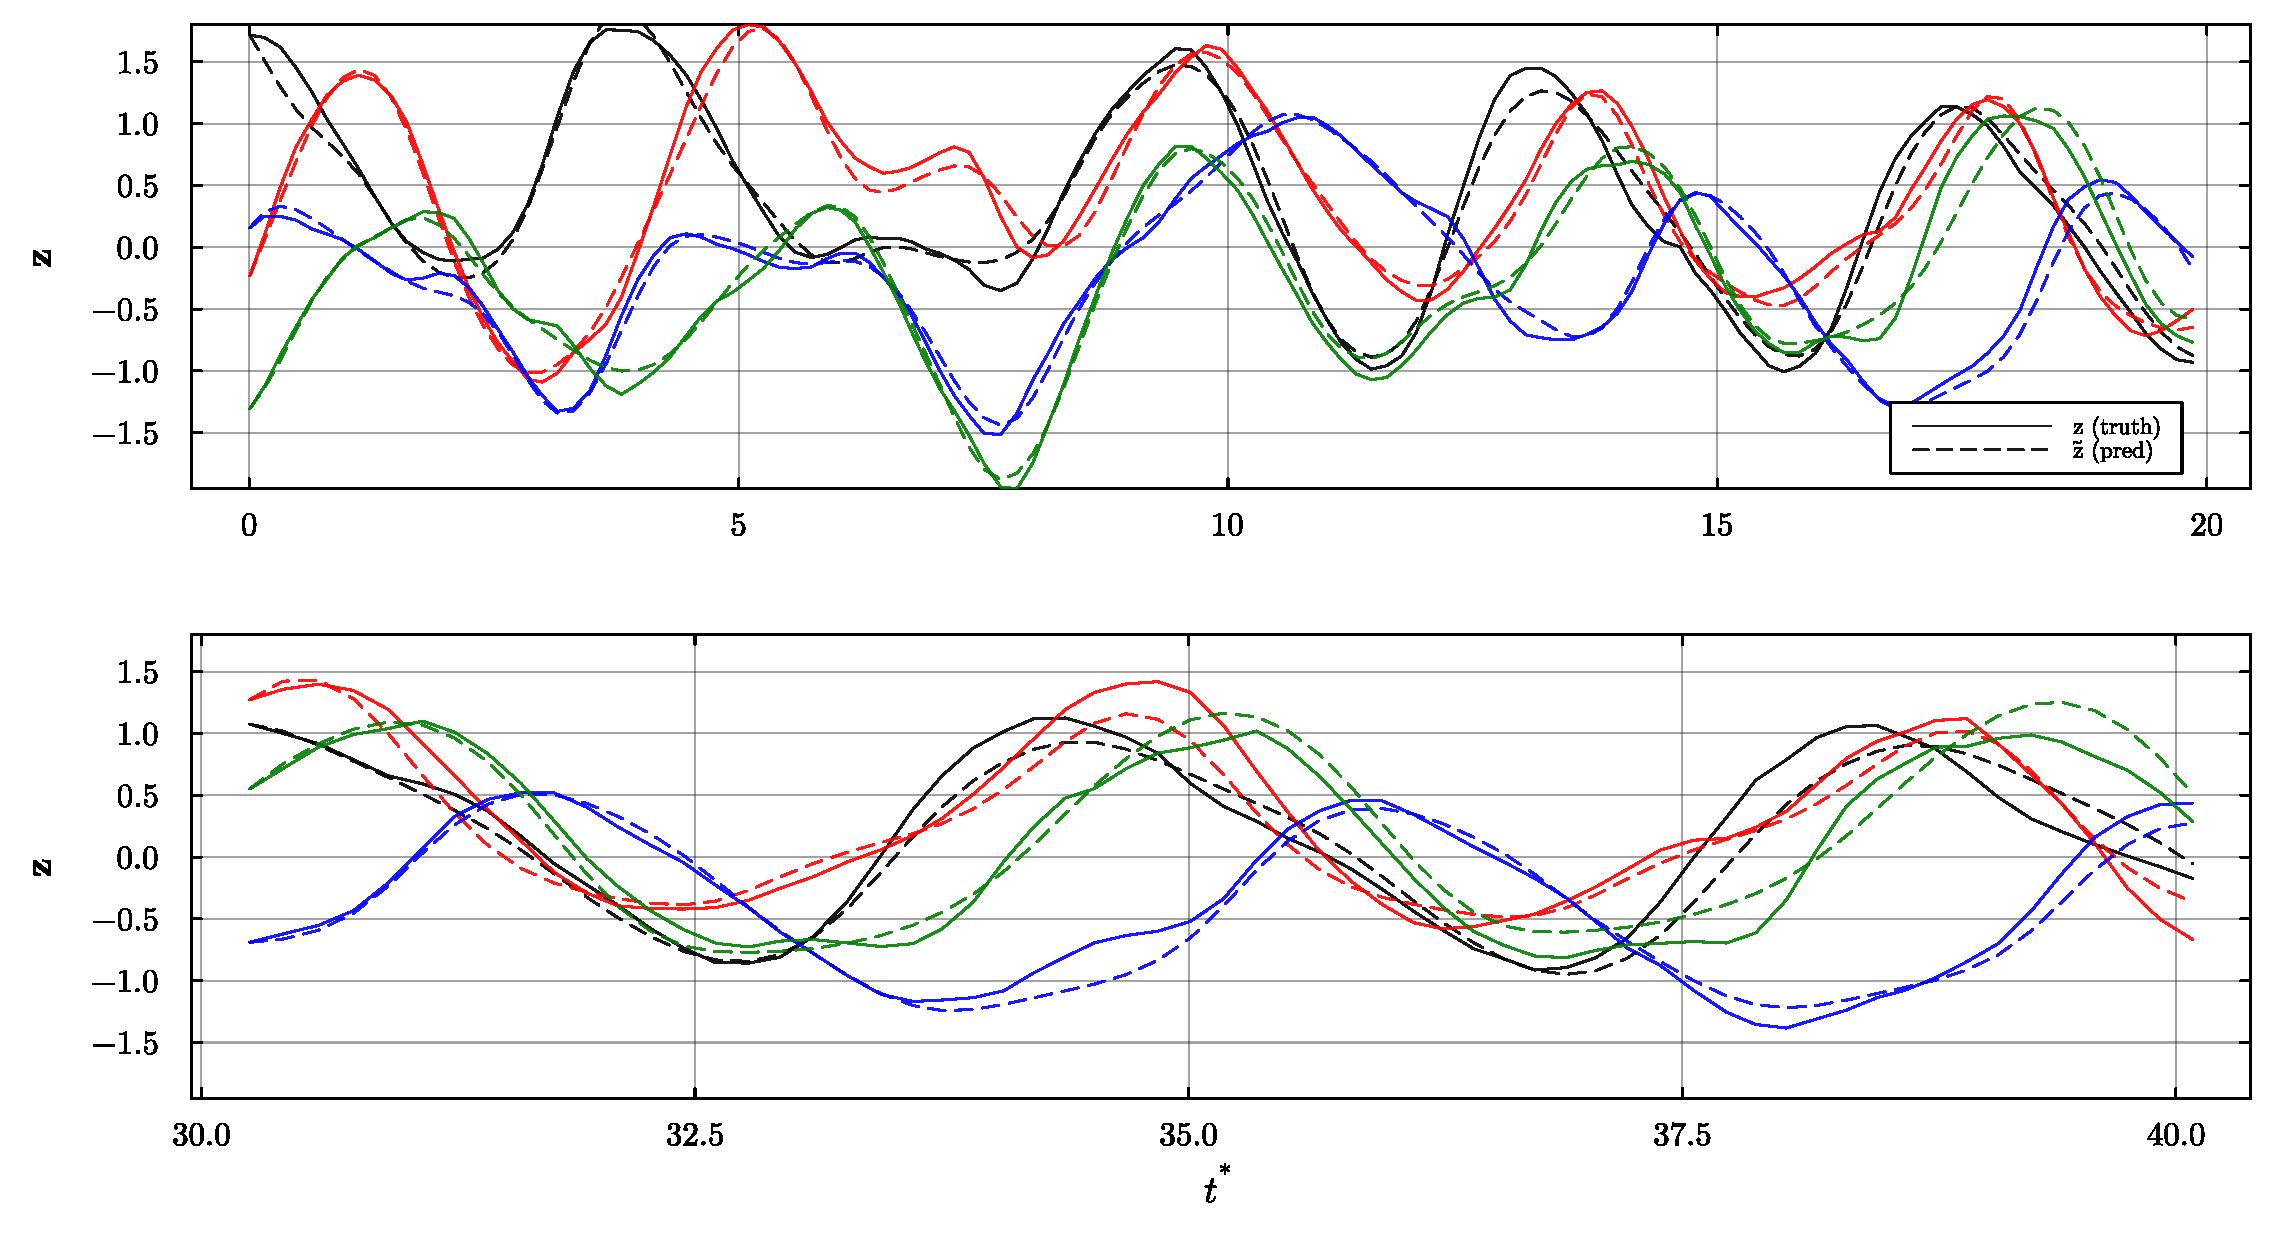
\includegraphics[width=\linewidth]{figures/Results/base/rollout_multi.pdf}
    \caption{Single rollout from $t^*=0$ across both windows after the first retraining, no segment resets.}
    \label{fig: retrain_node_singleshoot}
    \end{subfigure}
    \caption{Latent dynamics of $f_\phi$ after the first retraining, four representative components shown over two time windows ($t^* \in [0,20]$, top; $t^* \in [30,40]$, bottom). Reference $z$ (solid) against prediction $\tilde{z}$ (dashed). (a) Converged multiple-shooting fit on the augmented trajectory set, with segment start/end markers; (b) unaided single rollout from $t^*=0$ over the same windows.}
    \label{fig: retrain_node_rollout}
\end{figure}

The converged multiple-shooting fit of the augmented set, \autoref{fig: retrain_node_ms}, is visibly looser than the initial fit in \autoref{fig: base_node_ms}: the shooting segments no longer overlap cleanly at their boundaries, and small discontinuities now appear at the group ends. This follows from the retraining scheme and is similar to the behaviour shown in \autoref{fig: combined_training_base}. The newly harvested trajectory is but a minority of the augmented set~\eqref{eq: traju_update}, so the averaged loss~\eqref{eq: node_loss_ms} stays dominated by the originally represented dynamics, and the shortened retraining schedule leaves not enough room for the shooting gaps to be pushed to zero.

The single rollout of \autoref{fig: retrain_node_singleshoot}, however, tracks the reference markedly better than the looser segment fit would suggest: integrated from $t^*=0$, $f_\phi$ holds phase and amplitude on the dominant components across both windows, with the mismatch only emerging towards the end of the span. Thus, the looser segment fit does not automatically translate into worse rollouts; the retrained $f_\phi$ has still absorbed the dominant latent dynamics of the extended horizon, which determine the rollout and the achievable acceleration.

After the second retraining, the trajectory set spans three disjoint chunks, shown in the bottom panels of \autoref{fig: retrain2_node_rollout}. The first two chunks remain well-fitted in both segments and the rollout, but the third is remarkably worse: its shooting segments leave visible gaps, and the rollout decorrelates early. Similar to the second retraining of the autoencoder, this is caused by the under-representation of the current flow state in the set, the chunk was harvested from the dissipative regime that rollouts~4--6 drove $\mathcal{S}$ into, and enters~\eqref{eq: traju_update} as a minority, so the averaged loss~\eqref{eq: node_loss_ms} stays dominated by the older dynamics and $f_\phi$ fits it only weakly, the same effect behind the immediate KNN trigger of rollout~7.


 \begin{figure}[htbp]
    \centering
    \begin{subfigure}[t]{0.48\textwidth}
        \centering
        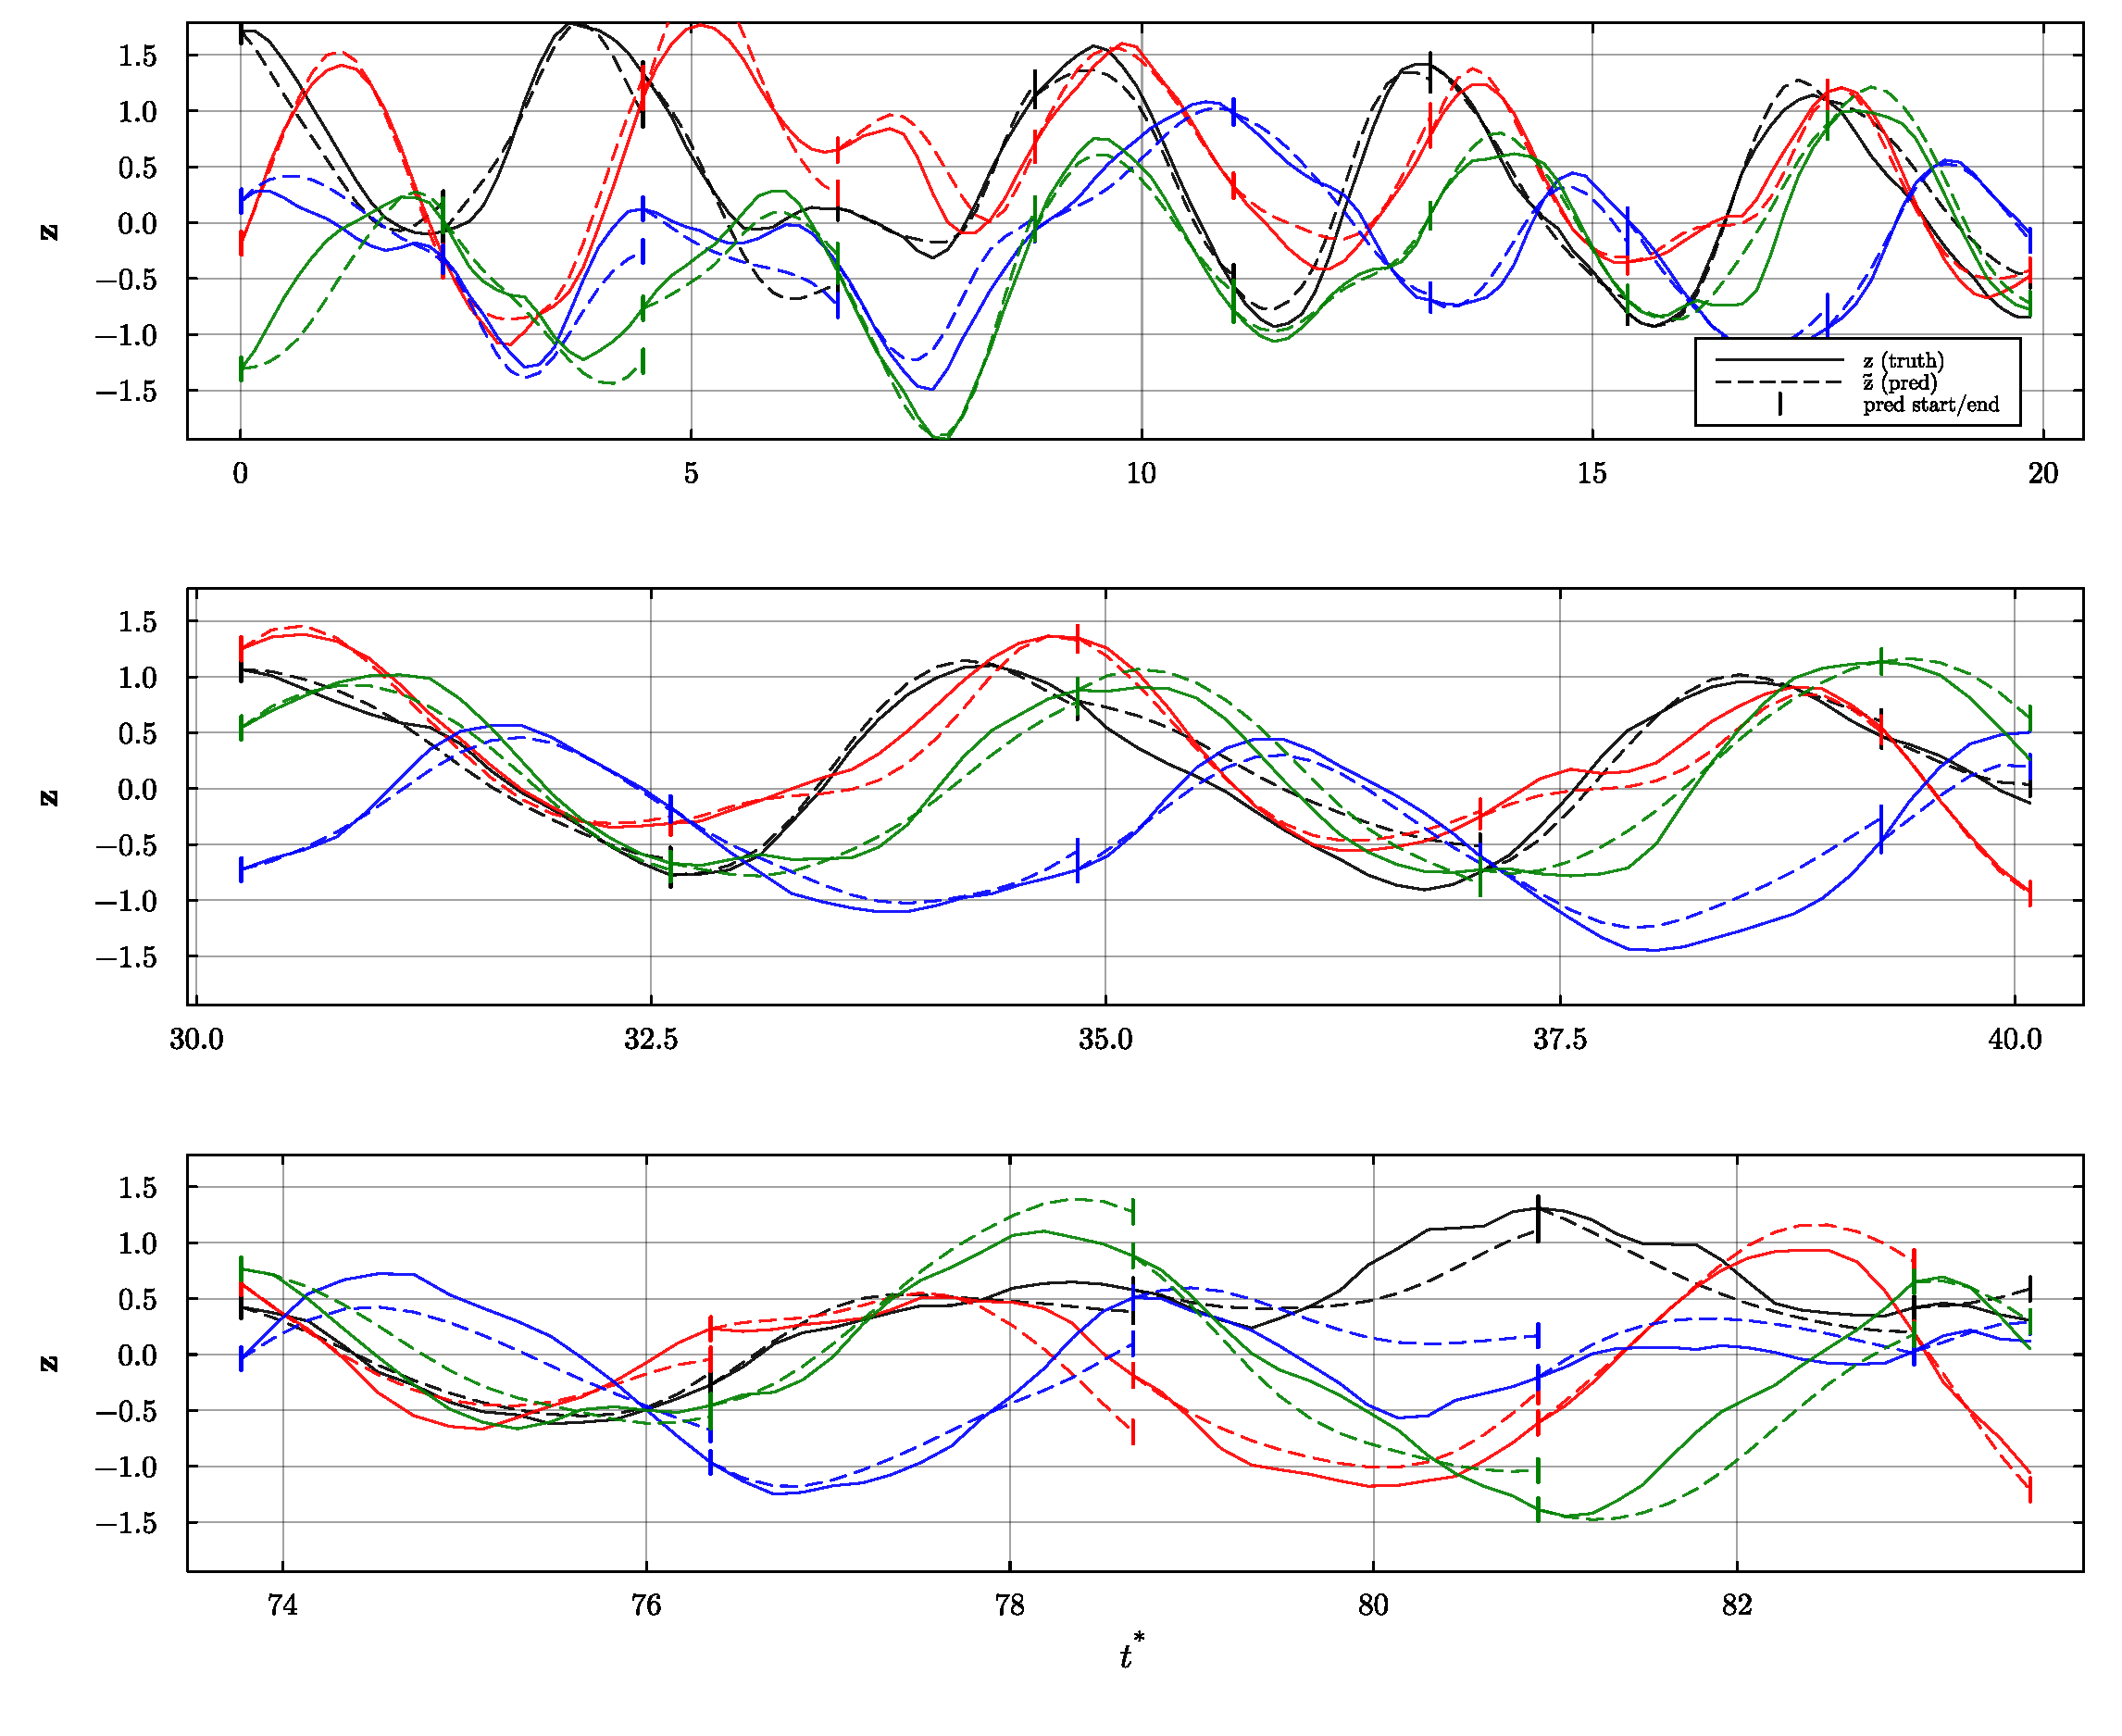
\includegraphics[width=\linewidth]{figures/Results/base/multiple_shoot_multi_2chunk.pdf}
    \caption{Converged multiple-shooting fit on the twice-augmented trajectory set; markers denote shooting-segment boundaries.}
    \label{fig: retrain2_node_ms}
    \end{subfigure}
    \hfill
    \begin{subfigure}[t]{0.48\textwidth}
        \centering
        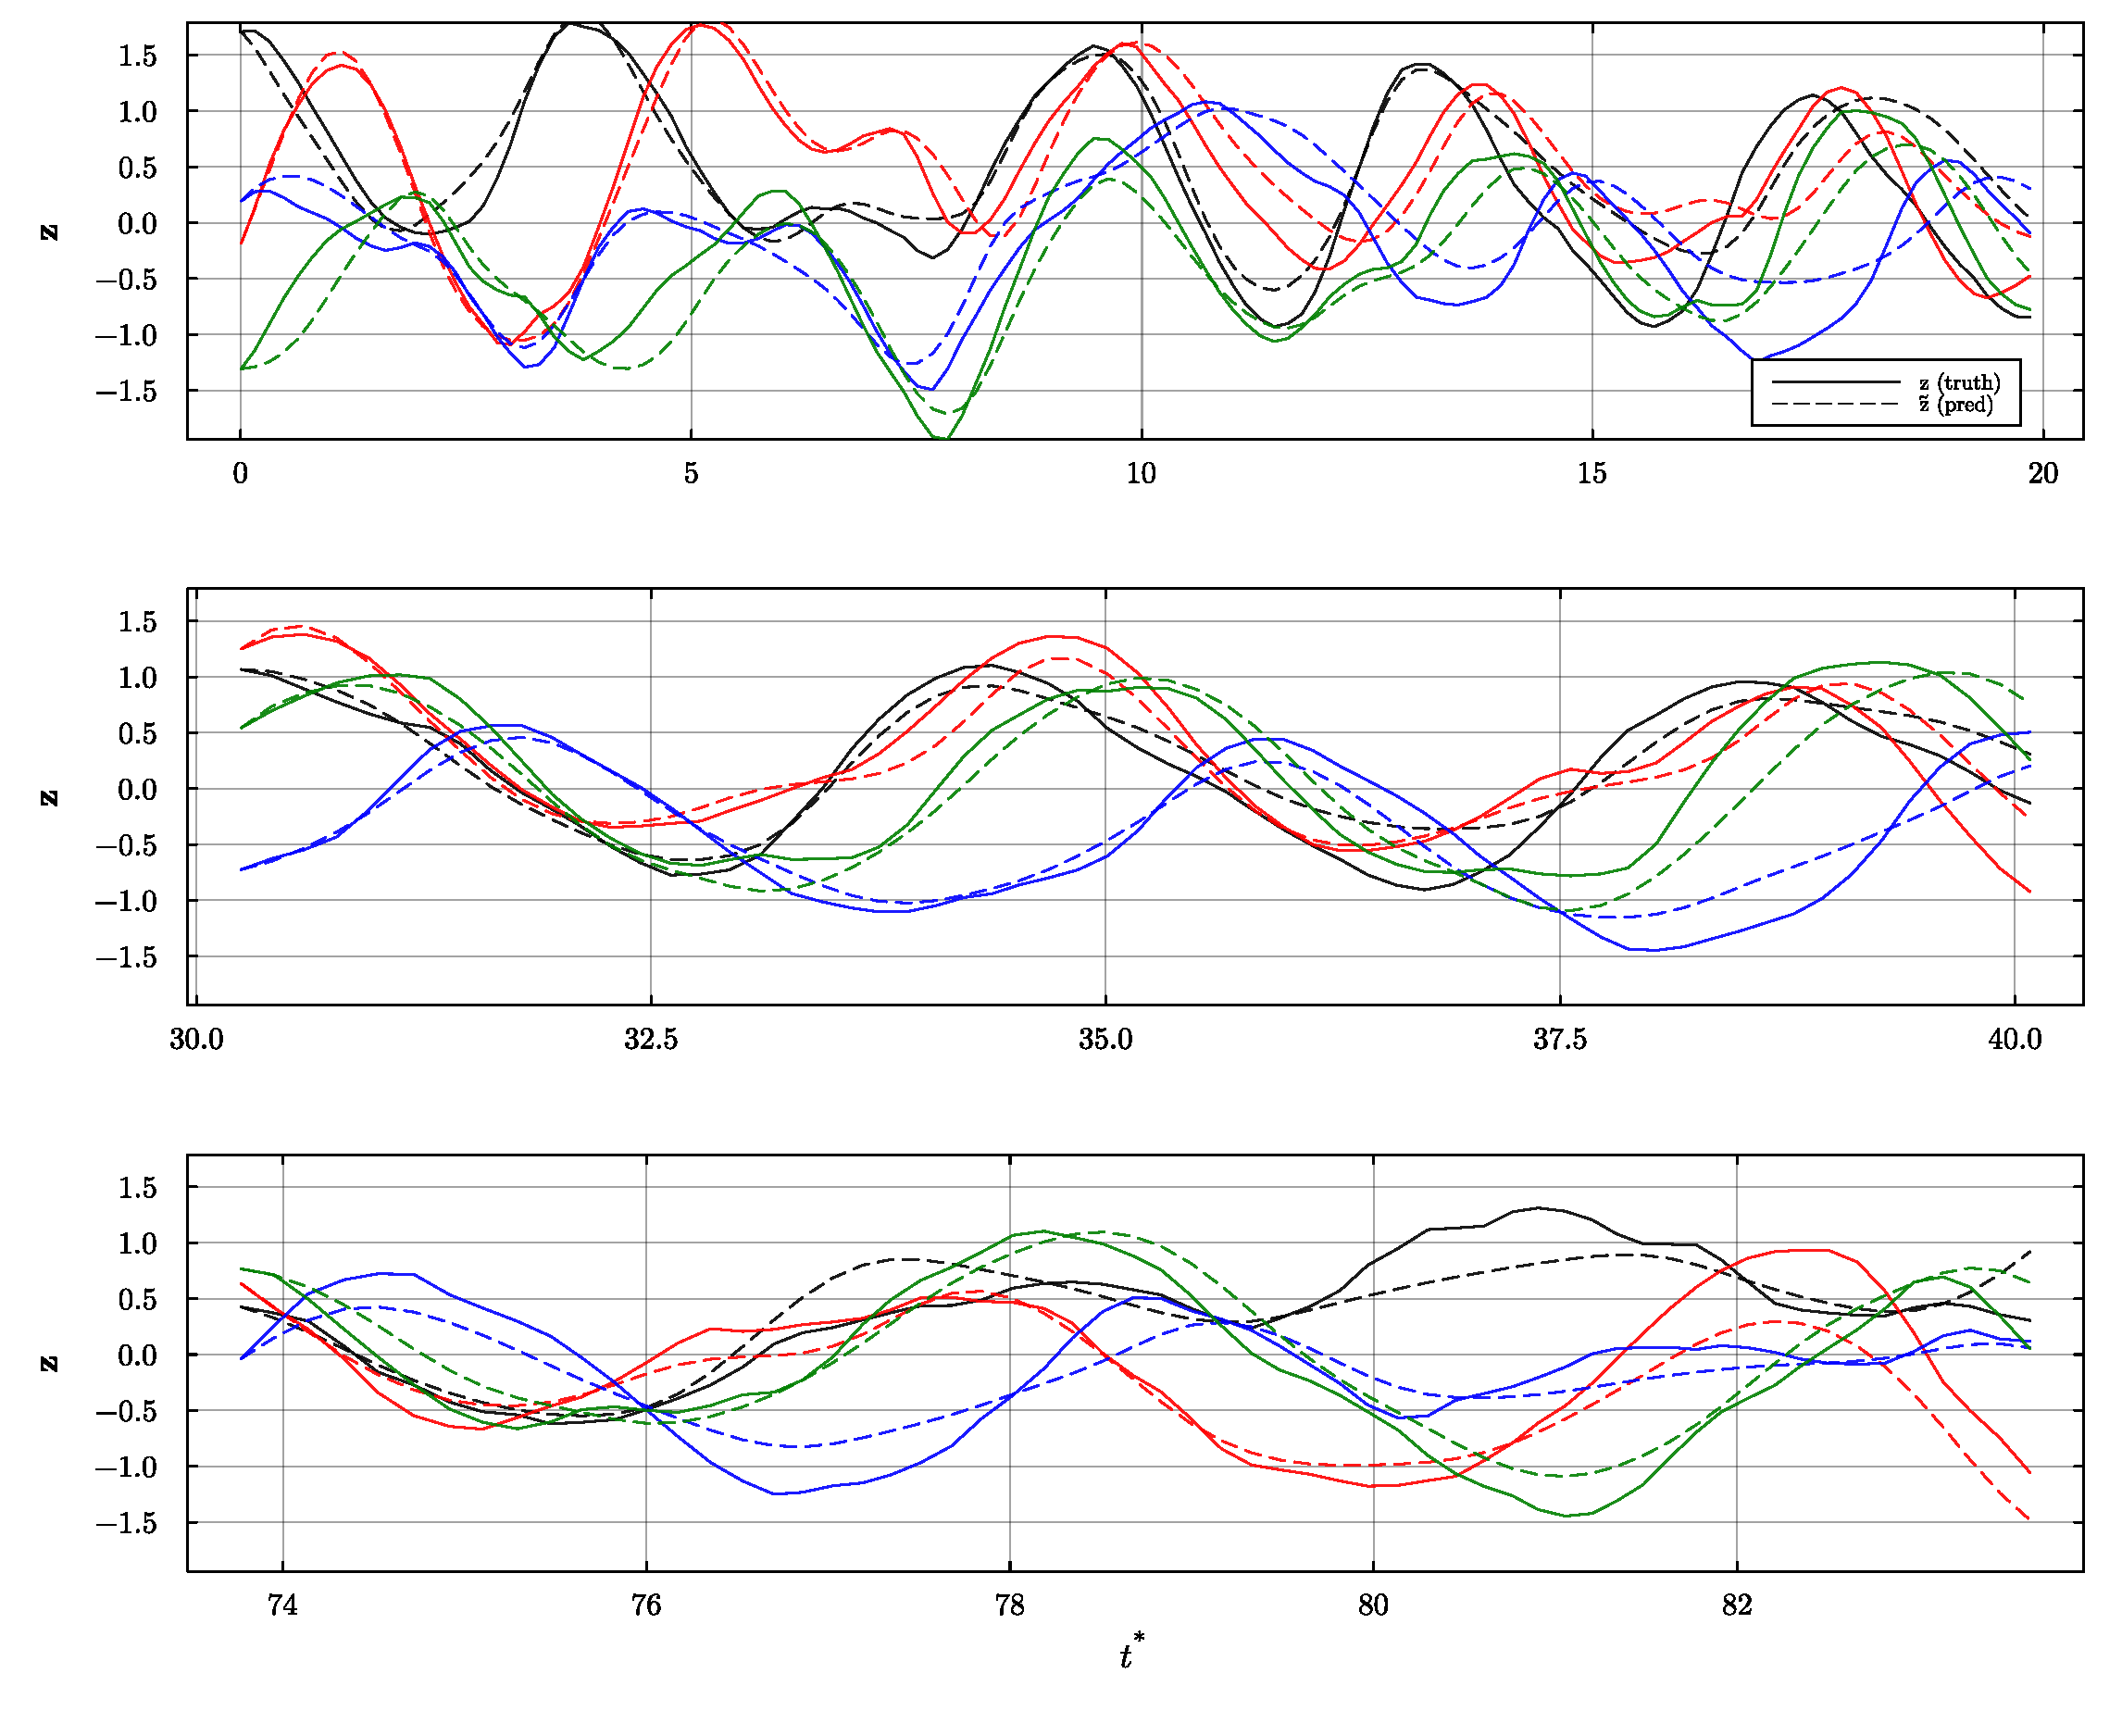
\includegraphics[width=\linewidth]{figures/Results/base/rollout_multi_2chunk.pdf}
    \caption{Single rollout from $t^*=0$ across all windows after the second retraining, no segment resets.}
    \label{fig: retrain2_node_singleshoot}
    \end{subfigure}
    \caption{Latent dynamics of $f_\phi$ after the second retraining, four representative components shown over three time windows ($t^* \in [0,20]$, top; $t^* \in [30.24,40.24]$, middle; $t^* \in [73.77, 83.77]$, bottom). Reference $z$ (solid) against prediction $\tilde{z}$ (dashed). (a) Converged multiple-shooting fit on the augmented trajectory set, with segment start/end markers; (b) unaided single rollout from $t^*=0$ over the same windows.}
    \label{fig: retrain2_node_rollout}
\end{figure}

The behaviour of $f_\phi$ across the hybrid simulation shows that the temporal error can have two origins. The first is, as mentioned in \autoref{sect: KNN}: even a well-converged fit sustains the latent dynamics only over a limited horizon before the rollout drifts from the reference, partly through the autoregressive nature of the neural ODE, and partly through the chaotic divergence of the wake itself, which is why the rollout must be gated rather than trusted indefinitely. The second matches the conclusions from \autoref{subsect: 4_ae_performance}: the fidelity of each retrained $f_\phi$ is set by how well the active flow regime is represented in $\boldsymbol{\mathcal{T}}_z$, so the well-covered early trajectories are reproduced accurately while the under-represented later trajectories are fitted only weakly. The retraining procedure effectively transfers the dominant dynamics when the new data follow the existing distribution, but degrades when they do not. The influence of a relevant governing hyperparameter, the group size $n_s$ on the rollout fidelity is examined next in \autoref{subsect: 4_node_params}.

\section{Effect of Pipeline Parameters}
\label{sect: 4_p_parameters}

Having discussed the functioning of the hybrid simulation and its physical effects in detail in \autoref{sect: 4_base_hybrid}, this section aims to highlight the influence of specific parameters of each component of $\mathcal{P}$  $(\varphi_\theta,\,\psi_\theta,\,f_\phi,\,\mathcal{K})$. Where certain parameters are isolated to quantify their effects, with two aims: to justify the baseline values of \autoref{tab: 4_hybrid_config} rather than presenting them arbitrarily, and to expose the trade-offs that lie within the developed framework. The study proceeds component by component, following the order of \autoref{chap: Methodology}. For the autoencoder, the latent dimension $N_z$ and the initial number of autoencoder training epochs are varied to examine their influence on the hybrid simulation across its respective time window. For the Neural ODE, the influence of the multiple-shooting group size $n_s$ is displayed, since it directly governs rollout stability and $f_\phi$ learning capabilities. For the integration monitor, the effect of the relative threshold quantile $q$ is shown, as it directly influences the rollout length. 

The parameters presented in this section are those that have the greatest influence on the main goal of the developed framework, namely, accelerating turbulent simulations. Because the developed framework comprises numerous parameters that can influence the acceleration and fidelity of the hybrid runs, not all are shown in this section. For an overview of all simulations that were run, and their relevant performance metrics, see \autoref{app: par_var}.

Each parameter is varied individually, following one-factor-at-a-time (OFAT) analysis, bout the baseline of \autoref{tab: 4_hybrid_config}; this means that the interactions between the parameters are not explored. A comprehensive study of the interactions between these parameters would require a large number of pipeline training runs, which would grow exponentially with the parameter count and exceed this work's computational budget. The parameter variations below, therefore, report the effect of each parameter, with the baseline serving as a solid comparison point. The following subsections will present and compare various hybrid simulations based on the comparison metrics presented in \autoref{subsect: 4_metrics}, the exact values that were used to construct these metrics (such as $T^\text{h, tot}_\text{wall}$ and $T^\text{h, training}_\text{wall}$) are presented in \autoref{app: par_var}.


\subsection{Autoencoder}
\label{subsect: 4_ae_parameters}

The autoencoder uses $\varphi_\theta$ to compress instantaneous velocity snapshots $\mathbf{u}$ down to the compressed representation $\mathbf{z}$. Although it is not a time-dependent operation, it does have a significant influence on the dynamics of $\boldsymbol{\mathcal{T}}_z$, since it controls how the full-scale physics are represented on the lower-dimensional latent space. This means that the $\varphi_\theta$ dictates the dynamics that $f_\phi$ has to learn, which get rolled out by the ODE solver past the training horizon as the rolled out trajectory $\tilde{\boldsymbol{\mathcal{T}}}_z$. Subsequently, these rolled-out dynamics are reconstructed in physical space by $\psi_\theta$, which in turn influences the downstream flow behaviour, which is fed back into $\mathcal{P}$ at later retrain or hybrid stages. 

To assess the influence of the autoencoder, three parameters are varied: the latent dimension $N_z$, the number of initial training epochs, and the physics-informed loss weighting.

\subsubsection{Latent dimension}
The latent dimension $N_z$ determines the width of the bottleneck and governs how much of the flow physics is preserved by the compression operation. \textcite{Nair2024} has shown that for autoencoder--neural ODE surrogates of advection-dominated flows, the recovered latent time-scales are governed primarily by the training-trajectory length rather than by $N_z$, so that the bottleneck width has little bearing on how long the latent rollout remains temporally faithful. That work, however, evaluates accuracy in the latent prediction alone; it does not assess the fidelity of the full-scale field reconstructed from that latent state. The variation in latent dimensions here, therefore, serves to expose how $N_z$ trades the achievable acceleration against the fidelity of the reconstructed latent and full-scale dynamics.



In the present hybrid setting, $N_z$ instead trades inference speed against the fidelity of the reconstructed flow statistics, as the sweep over $N_z \in \{8, 16, 32\}$ (with $N_z = 16$ the baseline) in \autoref{fig: latent_speedup} shows. 

\begin{figure}[htbp]
  \centering
  \begin{tikzpicture}
    \begin{groupplot}[
        group style={group size=2 by 1, horizontal sep=1.7cm},
        width=6.2cm, height=6.0cm,
        symbolic x coords={8,16,32},
        xtick=data,
        xlabel={$N_z$},
        enlarge x limits=0.30,
        ymajorgrids=true,
        grid style={gray!30},
        nodes near coords,
        every node near coord/.append style={anchor=south, font=\footnotesize},
        tick label style={font=\small},
        label style={font=\small},
        title style={font=\small\bfseries},
      ]
      \nextgroupplot[ybar, bar width=24pt, ylabel={$S_\mathrm{loop}$}, ymin=0, ymax=2.0,
                     title={Inference-loop speedup},
                     nodes near coords={\pgfmathprintnumber[fixed,precision=2]{\pgfplotspointmeta}}]
        % \addplot[draw=black, fill=blue!55] coordinates {(8,2.51) (16,1.48) (32,1.64)};
        \addplot[draw=black, fill=blue!55] coordinates {(8,1.78) (16,1.48) (32,1.43)};

        % \draw[dashed,gray] (axis cs:8,1) -- (axis cs:32,1)
        %   node[pos=0.5,above,font=\scriptsize\itshape,gray,inner sep=1pt]{break-even};
      \nextgroupplot[ybar, bar width=24pt, ylabel={$S_\mathrm{eff}$}, ymin=0, ymax=0.1,
                     ytick={0,0.025,0.05,0.075,0.1,0.125},
                     scaled y ticks=false,
                     yticklabel style={/pgf/number format/fixed, /pgf/number format/precision=3},
                     title={Effective speedup (incl.\ training)},
                     nodes near coords={\pgfmathprintnumber[fixed,precision=3]{\pgfplotspointmeta}}]
        % \addplot[draw=black, fill=orange!75] coordinates {(8,0.113) (16,0.058) (32,0.069)};
        \addplot[draw=black, fill=orange!75] coordinates {(8,0.080) (16,0.073) (32,0.064)};

    \end{groupplot}
  \end{tikzpicture}
  \caption{Effect of the autoencoder latent dimension on hybrid solver acceleration. Left: inference-loop speedup $S_\mathrm{loop}$;  Right: effective speedup $S_\mathrm{eff}$, including training costs.}
  \label{fig: latent_speedup}
\end{figure}

The smallest bottleneck proves to be the best of the three models in terms of acceleration performance: with $N_z=8$, the hybrid loop achieves $S_\text{loop} = 1.78$, compared with $1.48$ and $1.43$ for $N_z=16$ and $32$. The acceleration performance is largely attributable to the longer average rollout length of the smallest bottleneck, with an average of $964$ CFD steps per accepted prediction, compared to $408$ and $421$ for $N_z = 16$ and $32$, respectively. The fact that $N_z = 16$ still attains a marginally higher $S_\text{loop}$ than $N_z = 32$ despite a slightly shorter mean rollout, which reflects the lower per-step cost of advancing and decoding the narrower latent state. The lower-dimensional latent space presents simpler dynamics for the compact MLP $f_\phi$ to learn, so the rollout $\tilde{\boldsymbol{\mathcal{T}}}_z$ stays in distribution for longer before the KNN monitor flags it. This extended in-distribution horizon, and thus not any change in the intrinsic latent time-scale, is the dominant source of the higher $S_\text{loop}$ at small $N_z$; the latent dynamics are not slower, only easier to learn for both $f_\phi$ and the KNN monitor, which is consistent with \textcite{Nair2024}. However, because of the lower amount of values that are able to contain information about the chaotic flow, it is not able to produce the same result when assessed over mean flow and RST accuracy, as displayed in \autoref{fig: latent_field_mae}.


\begin{figure}[htp]
    \centering
    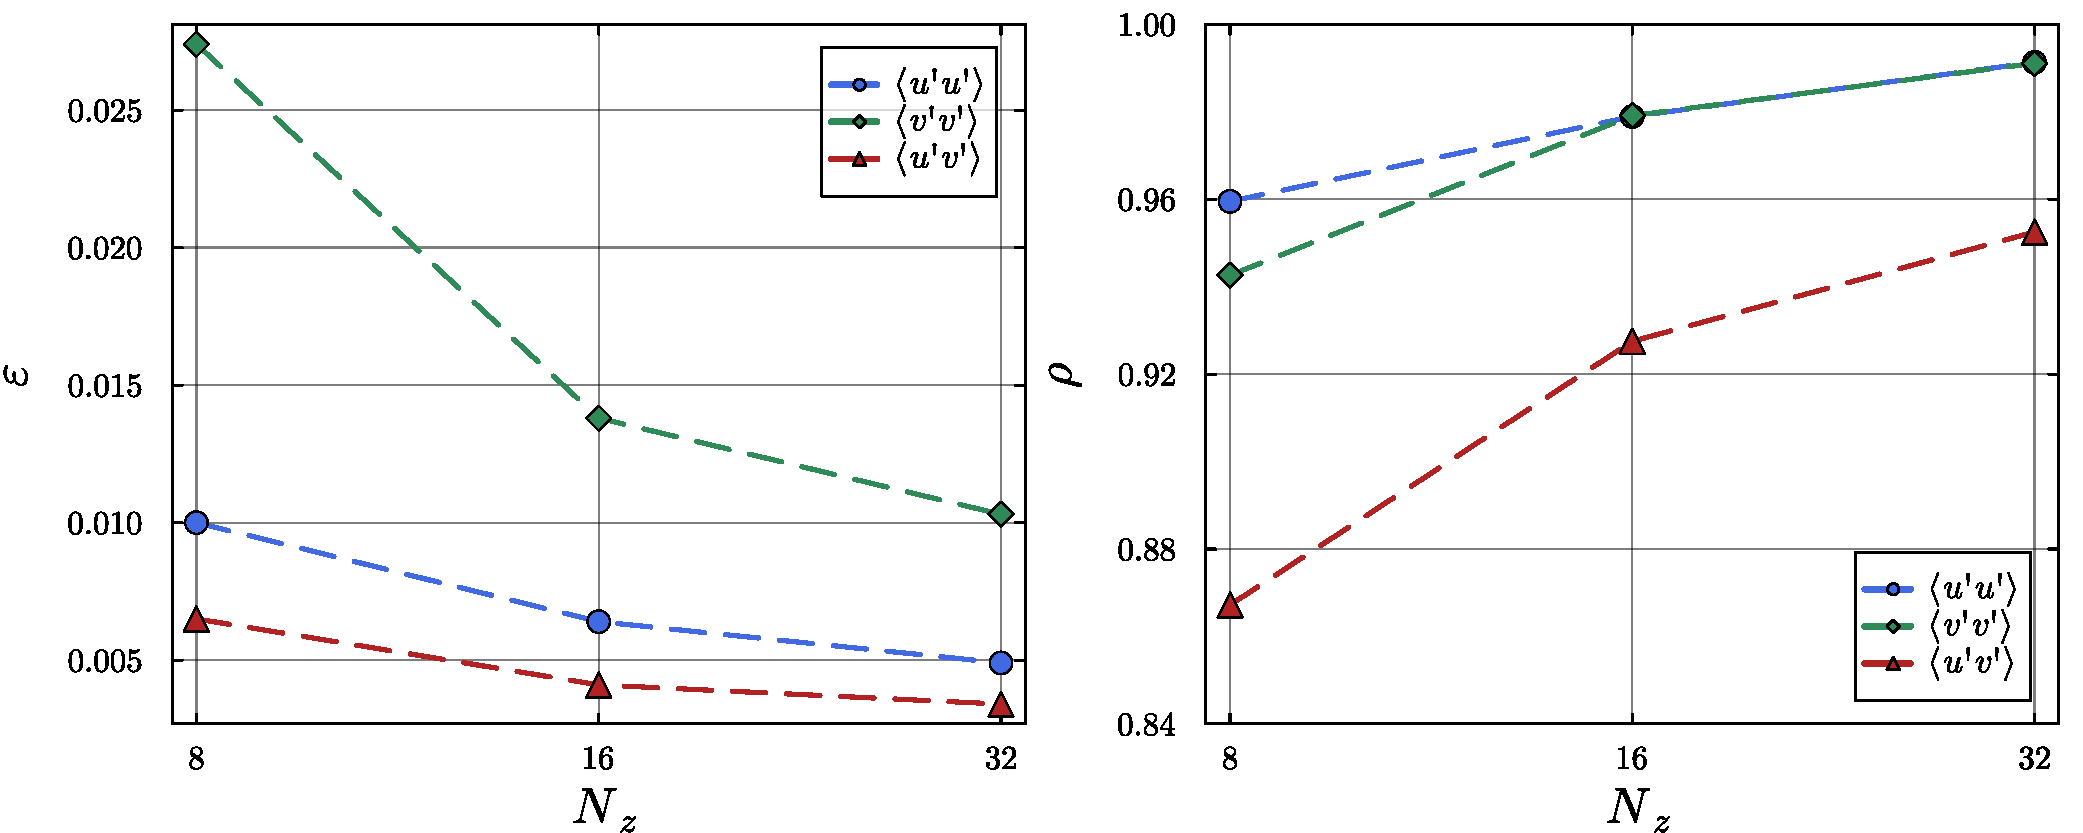
\includegraphics[width=\linewidth]{figures/Results/latent_rst_comp.pdf}
    \caption{Effect of the autoencoder latent dimension $N_z$ on the accuracy of the reconstructed Reynolds-stress field. Left: mean absolute error $\varepsilon$ of the three independent Reynolds-stress components. Right: spatial correlation coefficient $\rho$ of the same components. Both metrics improve monotonically with $N_z$, showing how the shear stress $\langle u'v' \rangle$ is the least well-recovered component at every bottleneck width.}
    \label{fig: latent_field_mae}
\end{figure}

As expected, a smaller latent space translates into less of the flow characteristics that are able to be passed down to $\varphi_\theta$, and reconstructed by $\psi_\theta$. \autoref{fig: latent_field_mae} shows that this loss is carried almost entirely by the second-order statistics. As the bottleneck widens, both panels improve with $N_z$, the field error $\varepsilon$ falls, and the spatial correlation $\rho$ rises for every Reynolds-stress component. The degradation is most severe for the spanwise normal stress $\langle v'v' \rangle$ of the RST, whose error nearly triples relative to $N_z = 32$ ($\varepsilon = 0.027$ against $0.010$). The correlation coefficients show that the shear stress $\langle u'v' \rangle$ is the least well recovered, especially for the smallest bottleneck. 

This comparison shows the trade-off the bottleneck imposes between speedup and the physical fidelity of the reconstructed turbulence statistics. At $N_z = 8$, the simpler latent dynamics produce by far the longest rollouts and the largest $S_\text{loop}$, but at the expense of the RST fields; the $N_z = 32$ shows that more complex latent dynamics allow for better turbulent reconstructions, but at the expense of a lesser acceleration performance. This means that the appropriate bottleneck size is thus dictated by whether statistical fidelity or acceleration behaviour is the priority for a given application. 

\subsubsection{Training Epochs}
The number of training epochs is varied around the baseline of $500$, since the autoencoders' initial training consumes most of the wall time, as \autoref{tab: wall_timing_hybrid} shows, but it also controls how strictly the instantaneous dynamics are learned, and therefore how the fluctuating field is represented in the latent space. The epoch count $E$ is swept over $E \in \{250, 500, 750\}$, with $E = 500$ the baseline; the retraining epochs are held fixed at $100$ throughout, so the sweep is meant to show the effect of the \emph{initial} compression quality.

\begin{figure}[htp]
  \centering
  \begin{tikzpicture}
    \begin{groupplot}[
        group style={group size=2 by 1, horizontal sep=1.7cm},
        width=6.2cm, height=6.0cm,
        symbolic x coords={250,500,750},
        xtick=data,
        xlabel={Epochs},
        enlarge x limits=0.30,
        ymajorgrids=true,
        grid style={gray!30},
        nodes near coords,
        every node near coord/.append style={anchor=south, font=\footnotesize},
        tick label style={font=\small},
        label style={font=\small},
        title style={font=\small\bfseries},
      ]
      \nextgroupplot[ybar, bar width=24pt, ylabel={$S_\mathrm{loop}$}, ymin=0, ymax=2.00,
                     title={Inference-loop speedup},
                     nodes near coords={\pgfmathprintnumber[fixed,precision=2]{\pgfplotspointmeta}}]
        % \addplot[draw=black, fill=blue!55] coordinates {(250,2.08) (500,1.48) (750,1.55)};
        \addplot[draw=black, fill=blue!55] coordinates {(250,1.74) (500,1.48) (750,1.44)};
        % \draw[dashed,gray] (axis cs:8,1) -- (axis cs:32,1)
        %   node[pos=0.5,above,font=\scriptsize\itshape,gray,inner sep=1pt]{break-even};
      \nextgroupplot[ybar, bar width=24pt, ylabel={$S_\mathrm{eff}$}, ymin=0, ymax=0.11,
                     ytick={0,0.025,0.05,0.075,0.1,0.125},
                     scaled y ticks=false,
                     yticklabel style={/pgf/number format/fixed, /pgf/number format/precision=3},
                     title={Effective speedup (incl.\ training)},
                     nodes near coords={\pgfmathprintnumber[fixed,precision=3]{\pgfplotspointmeta}}]
        % \addplot[draw=black, fill=orange!75] coordinates {(250,0.111) (500,0.058) (750,0.059)};
        \addplot[draw=black, fill=orange!75] coordinates {(250,0.093) (500,0.073) (750,0.054)};
    \end{groupplot}
  \end{tikzpicture}
  \caption{Effect of initial training epochs of the autoencoder on hybrid solver acceleration. Left: inference-loop speedup $S_\mathrm{loop}$;  Right: effective speedup $S_\mathrm{eff}$, including training costs.}
  \label{fig: epoch_speedup}
\end{figure}

\autoref{fig: epoch_speedup} shows how the effect on the acceleration performance mirrors that of the latent dimensions. The least-converged model performs best: at $E = 250$, the hybrid loop reaches $S_\text{loop} = 1.74$, against $1.48$ at the baseline and $1.44$ at $E = 750$. Just as with the narrower bottleneck, the improvement is carried by the average rollout length: $623$ CFD steps per accepted prediction at $E = 250$, compared to $408$ and $391$ at $E = 500$ and $750$. An under-trained encoder has not yet learned the fine turbulent fluctuations, so it produces a smoother, lower-complexity latent representation; in turn, the dynamics that $f_\phi$ must reproduce are correspondingly simpler, leading to $\tilde{\boldsymbol{\mathcal{T}}}_z$ remaining in distribution for longer before the KNN monitor flags it as OOD. Reducing the training budget, therefore, affects the rollout length through the same mechanism as shrinking $N_z$: it lowers the effective information that can be stored in the flow's latent representation.

\begin{figure}[htp]
    \centering
    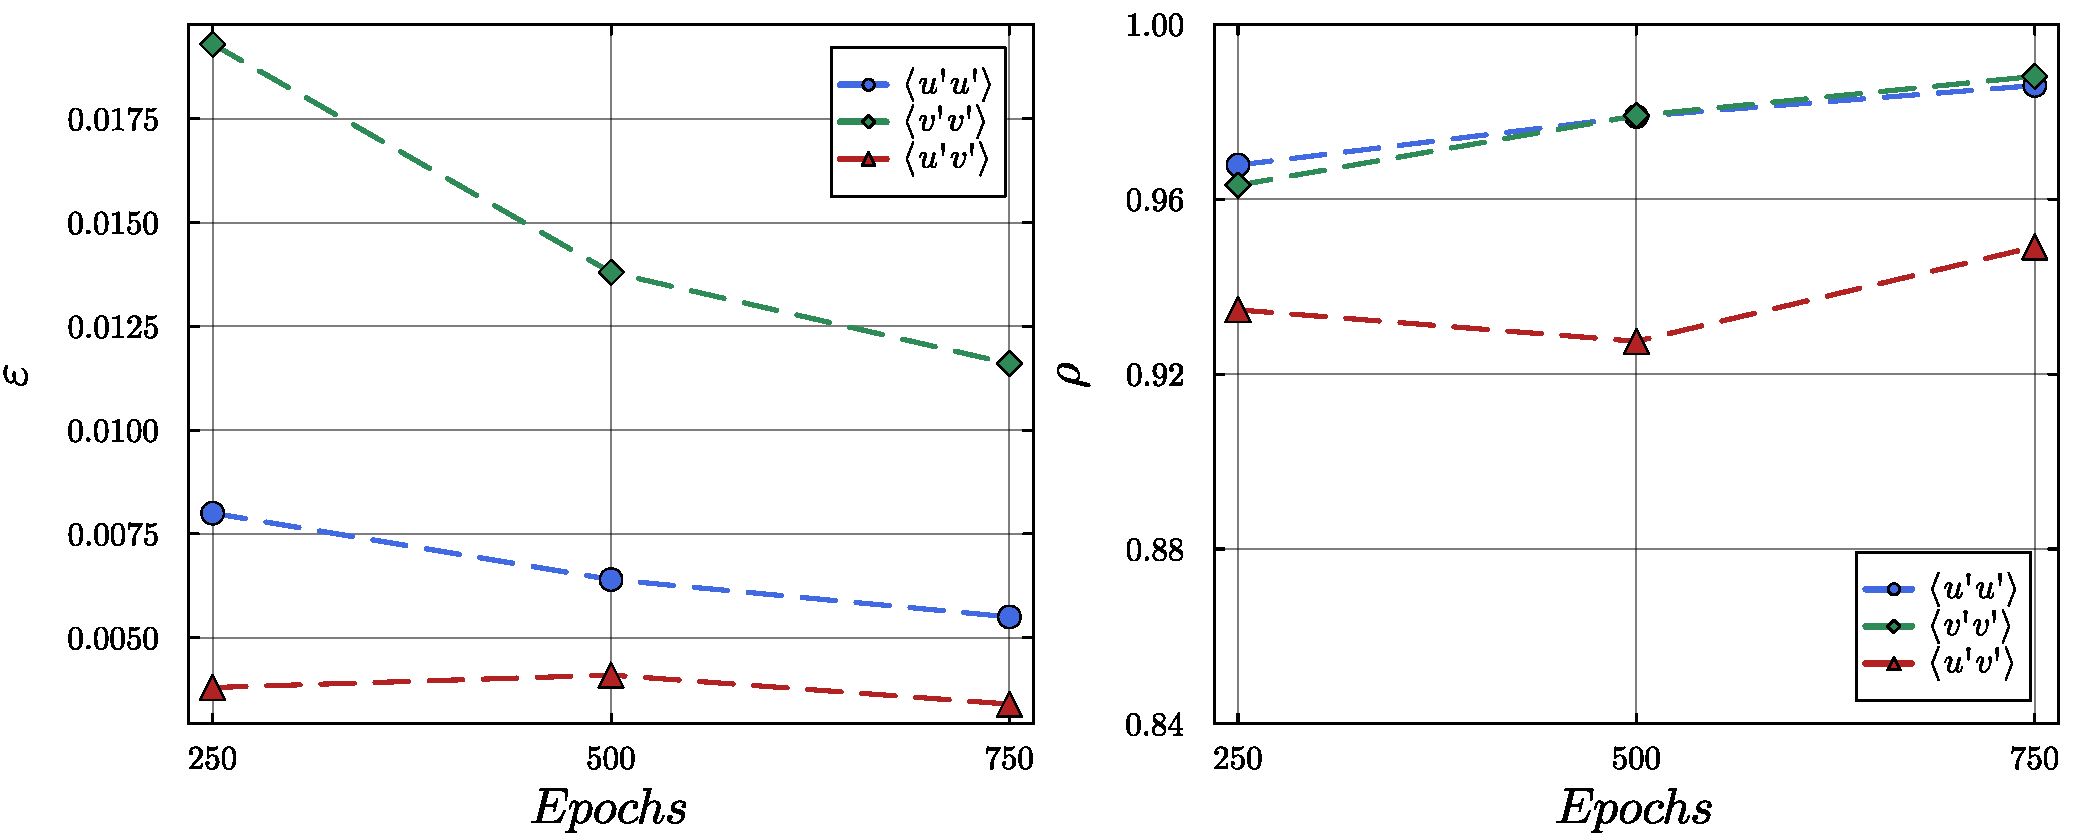
\includegraphics[width=\linewidth]{figures/Results/epoch_rst_comp.pdf}
    \caption{Effect of the initial autoencoder training epochs on the accuracy of the reconstructed Reynolds-stress field. Left: mean absolute error $\varepsilon$ of the three independent Reynolds-stress components. Right: spatial correlation coefficient $\rho$ of the same components. Increasing epoch count lowers $\varepsilon$, most strongly for $\langle v'v'\rangle$, while $\rho$ stays near unity}
    \label{fig: epoch_rst_comp}
\end{figure}

\autoref{fig: epoch_rst_comp} shows how the increase in epochs lowers the error in magnitude of the mean turbulent fluctuations, especially the transverse $\langle v'v' \rangle$ component. The spatial correlation $\rho$ is already high at $E = 250$ and barely changes. The encoder, therefore, captures the spatial pattern of the Reynolds stresses almost immediately, and the additional epochs mainly calibrate the fluctuation amplitude rather than relocate it. This behaviour can be highlighted when plotting the trajectory of the latent representation of the training window: 

\begin{figure}[htp]
    \centering
    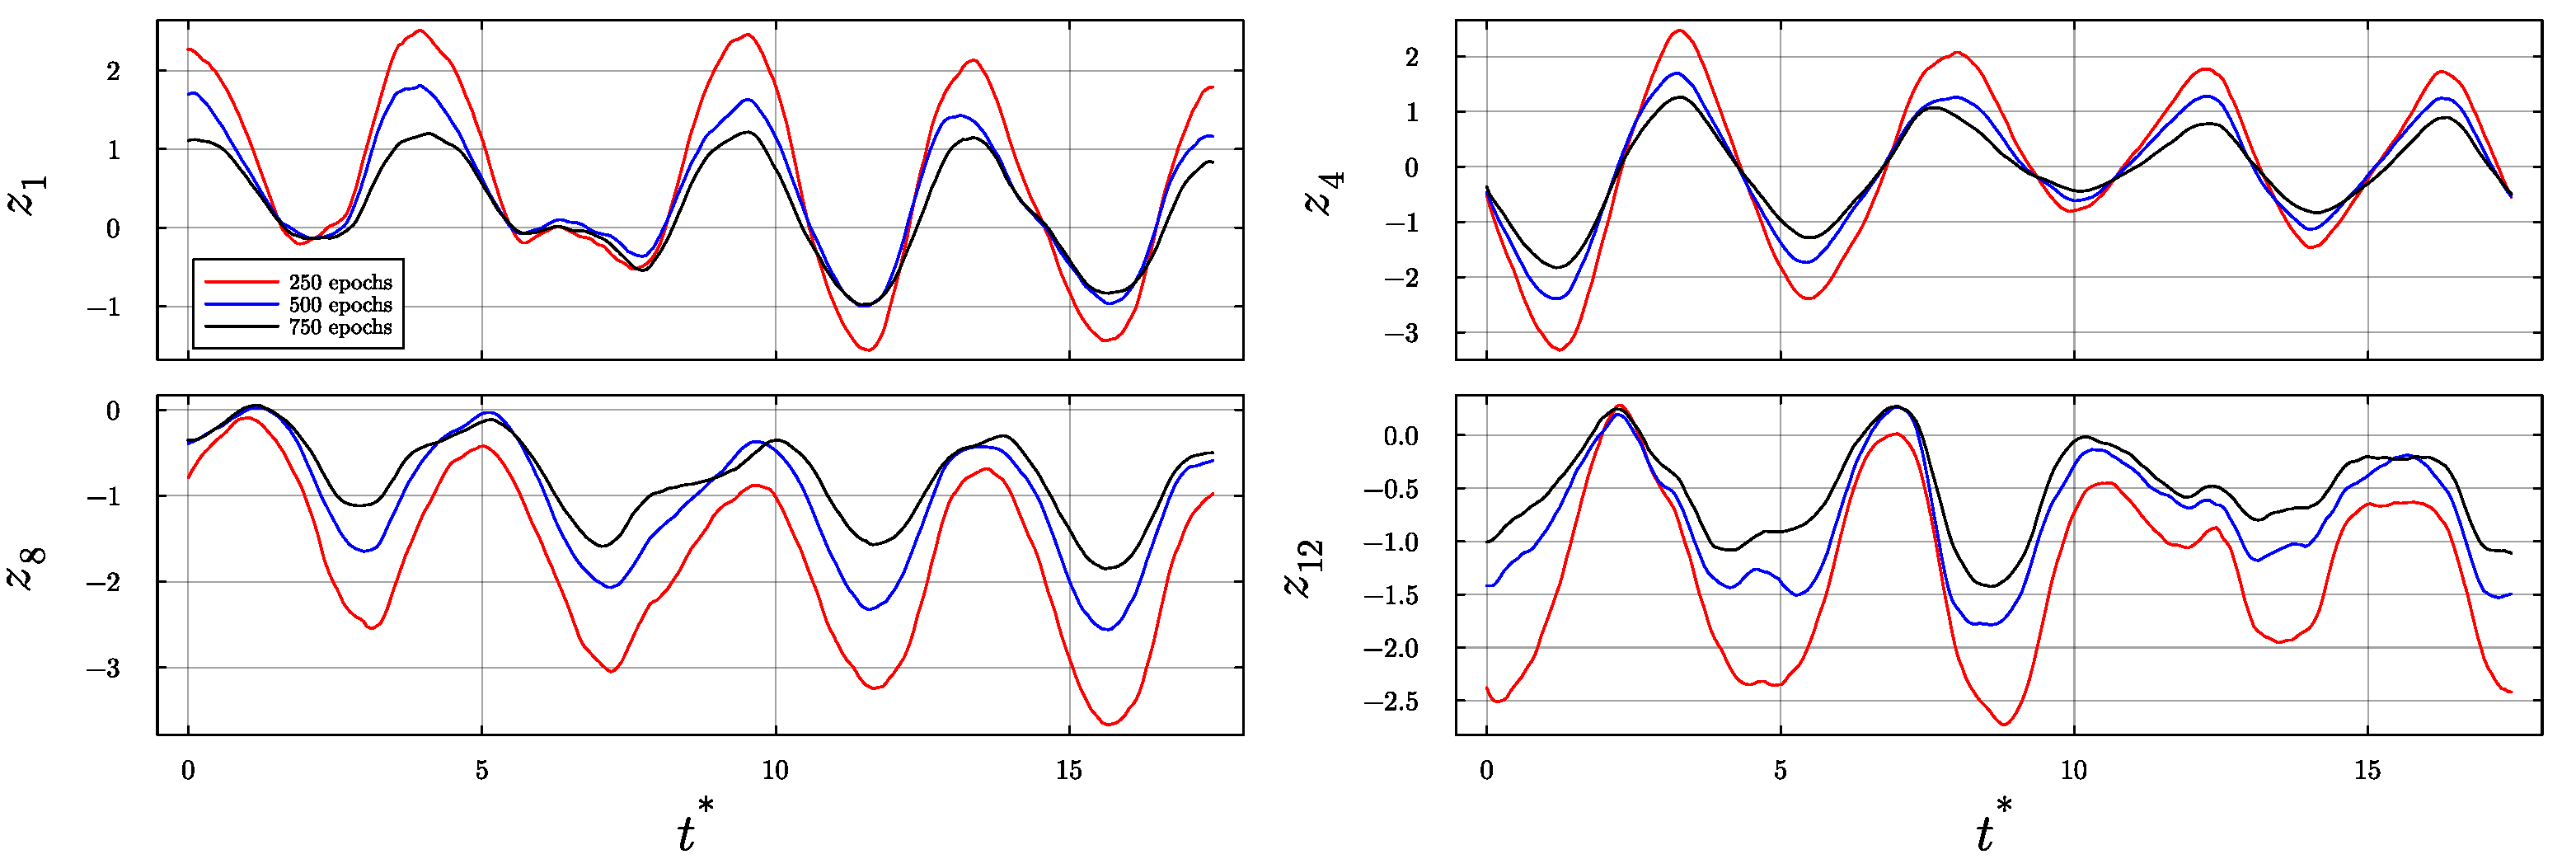
\includegraphics[width=\linewidth]{figures/Results/epoch_latent_comp.pdf}
    \caption{Four representative latent coordinates of the latent trajectory $\mathcal{T}_z$ for autoencoders trained $E = 250$ (red), $500$ (blue) and $750$ (black) epochs. The lower-epoch $\mathcal{T}_z$ has a higher amplitude than the higher-epoch trajectories, which appear to converge as $E$ increases.}
    \label{fig: latent_epochs}
\end{figure}

\autoref{fig: latent_epochs} confirms this conclusion. It shows how all three initial encoded trajectories trace the same dominant shedding oscillation, so the spatial pattern is shared, but the lower-epoch $\mathcal{T}_z$ oscillates at a higher amplitude that seems to converge as the number of epochs increases. The extra epochs thus mainly rescale the latent signal rather than reshape it; the rescaled amplitude is then translated to physical space by $\psi_\theta$, explaining the drop in $\varepsilon$ at near-constant $\rho$. The higher-amplitude, smoother $E = 250$ trajectory also provides the simpler dynamical target for $f_\phi$, which is why it sustains the longest average rollout.



\subsection{Neural ODE}
\label{subsect: 4_node_params}
The neural ODE $f_\phi$ integrates the latent state of the simulation over time during the latent rollout, so how long its prediction remains faithful to the reference sets directly determines how long the KNN monitor keeps the loop in distribution, and, with it, the achievable speedup. Two important hyperparameters of the multiple-shooting scheme \autoref{subsect: NODEtraining} govern this fidelity and are varied here: the group size $n_s$ and the continuity weight $\lambda_c$. 

\subsubsection{Group size}
The group size determines the length of the independent integrations that the trajectory is partitioned into: a small $n_s$ keeps the optimisation stable but multiplies the shooting boundaries and leaves little continuous latent horizon to be learnt, biasing the latent dynamics towards shorter rollouts. A lower $n_s$ also allows finer latent dynamical features to be learned for $f_\phi$. A larger $n_s$ will thus pass a smoother version of the latent dynamics to be learnt, with lower fidelity, but gives $f_\phi$ more time horizon to rollout over, which could improve the rollout length. 

\begin{figure}[htbp]
    \centering
    \begin{subfigure}[c]{0.48\textwidth}
        \centering
        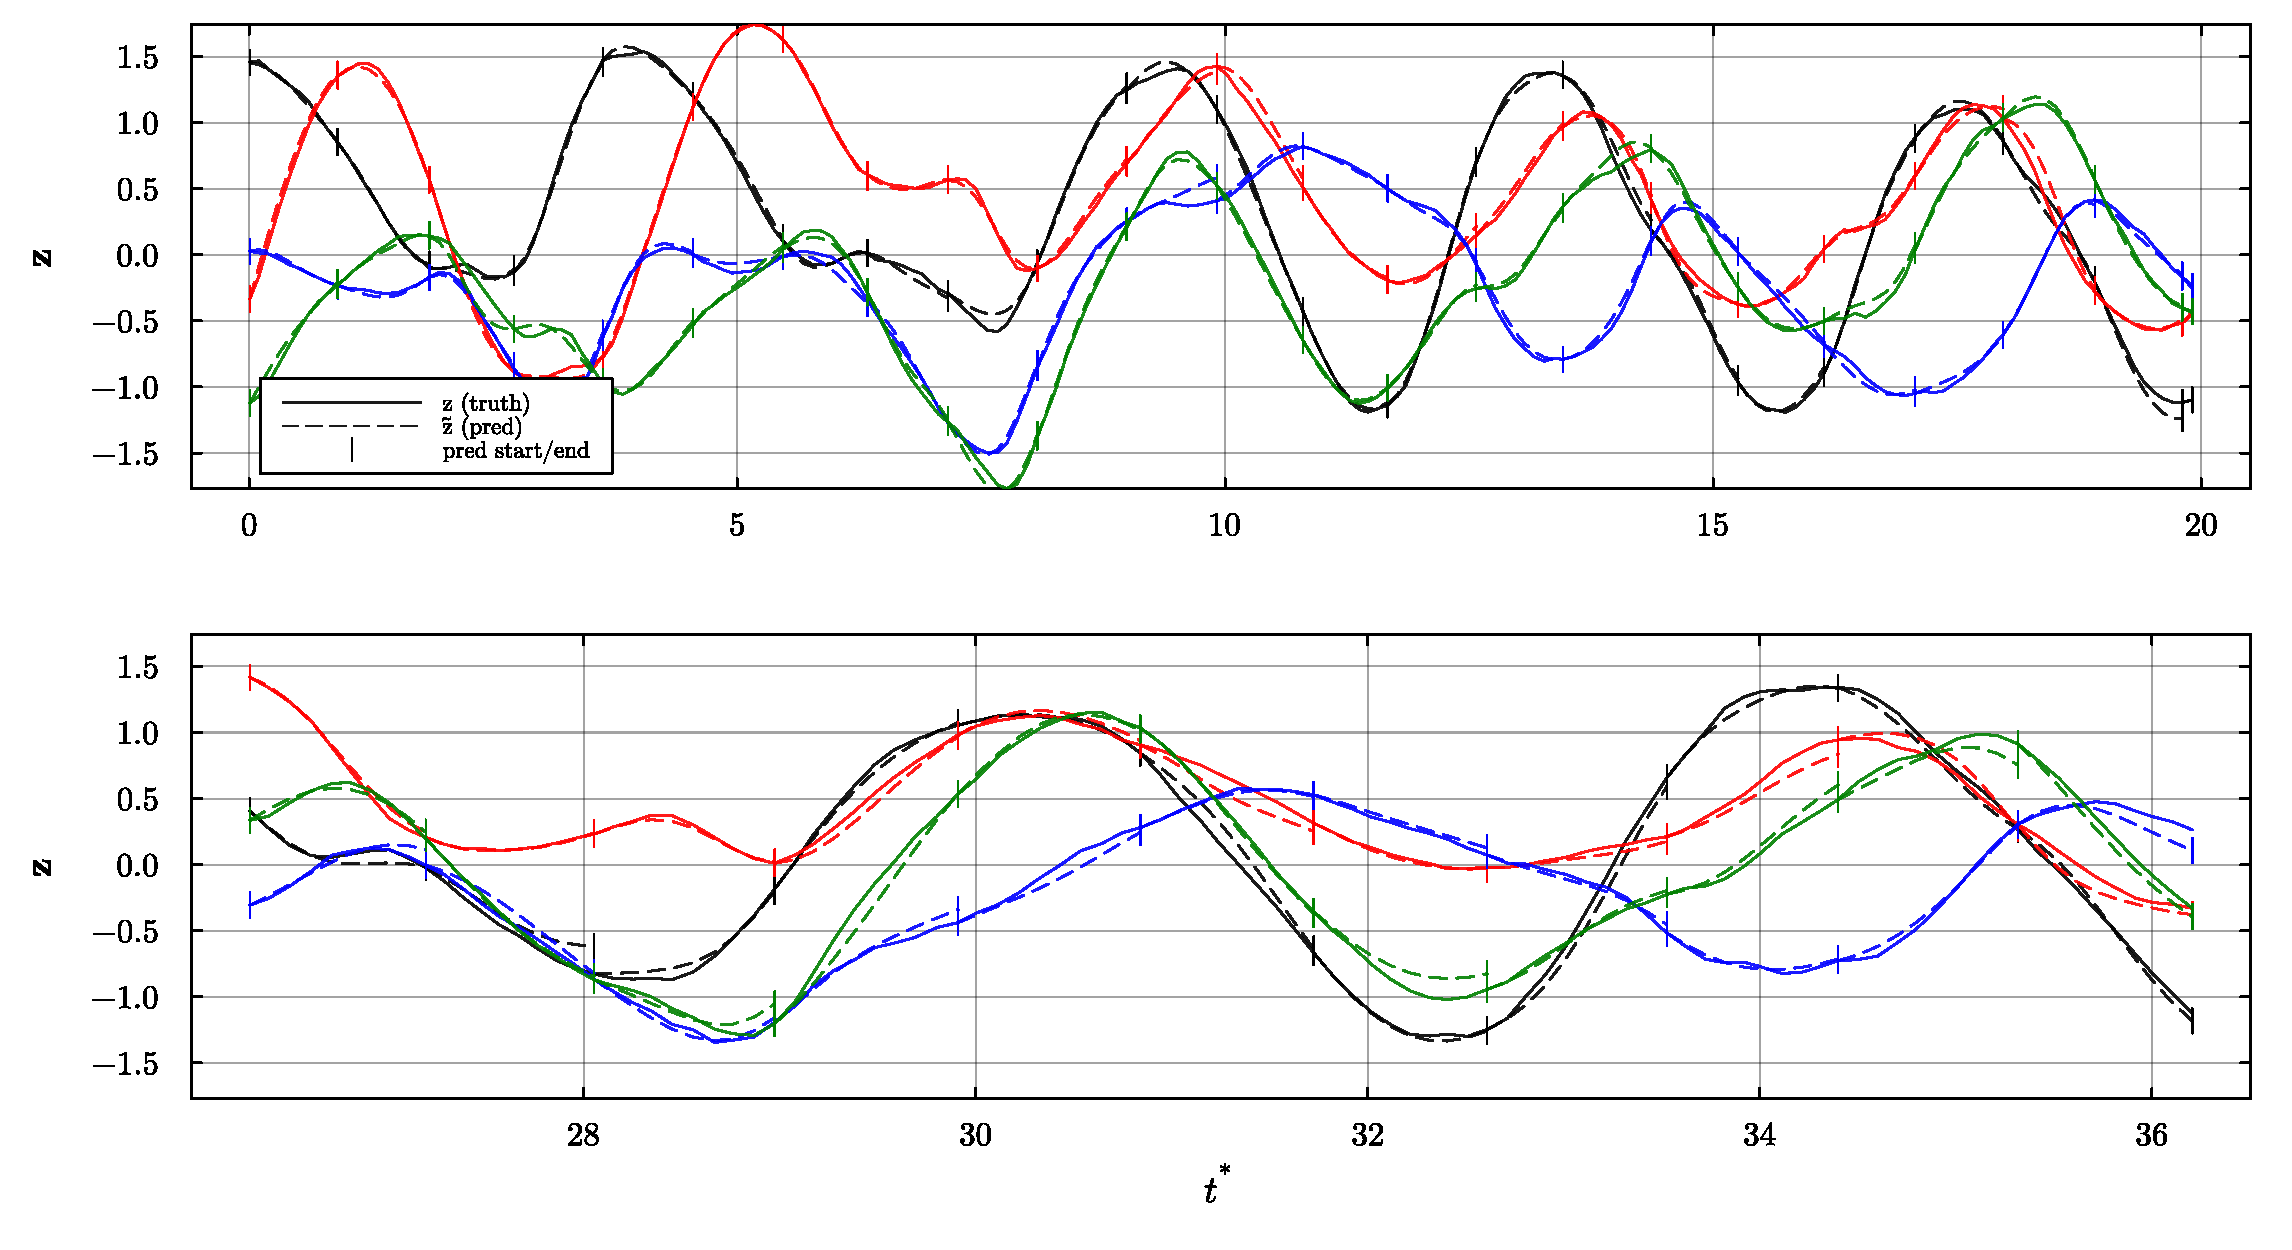
\includegraphics[width=\linewidth]{figures/Results/gs10_trajectories.pdf}
        \caption{}
        \label{fig: gs10_latent}
    \end{subfigure}
    \hfill
    \begin{subfigure}[c]{0.48\textwidth}
        \centering
        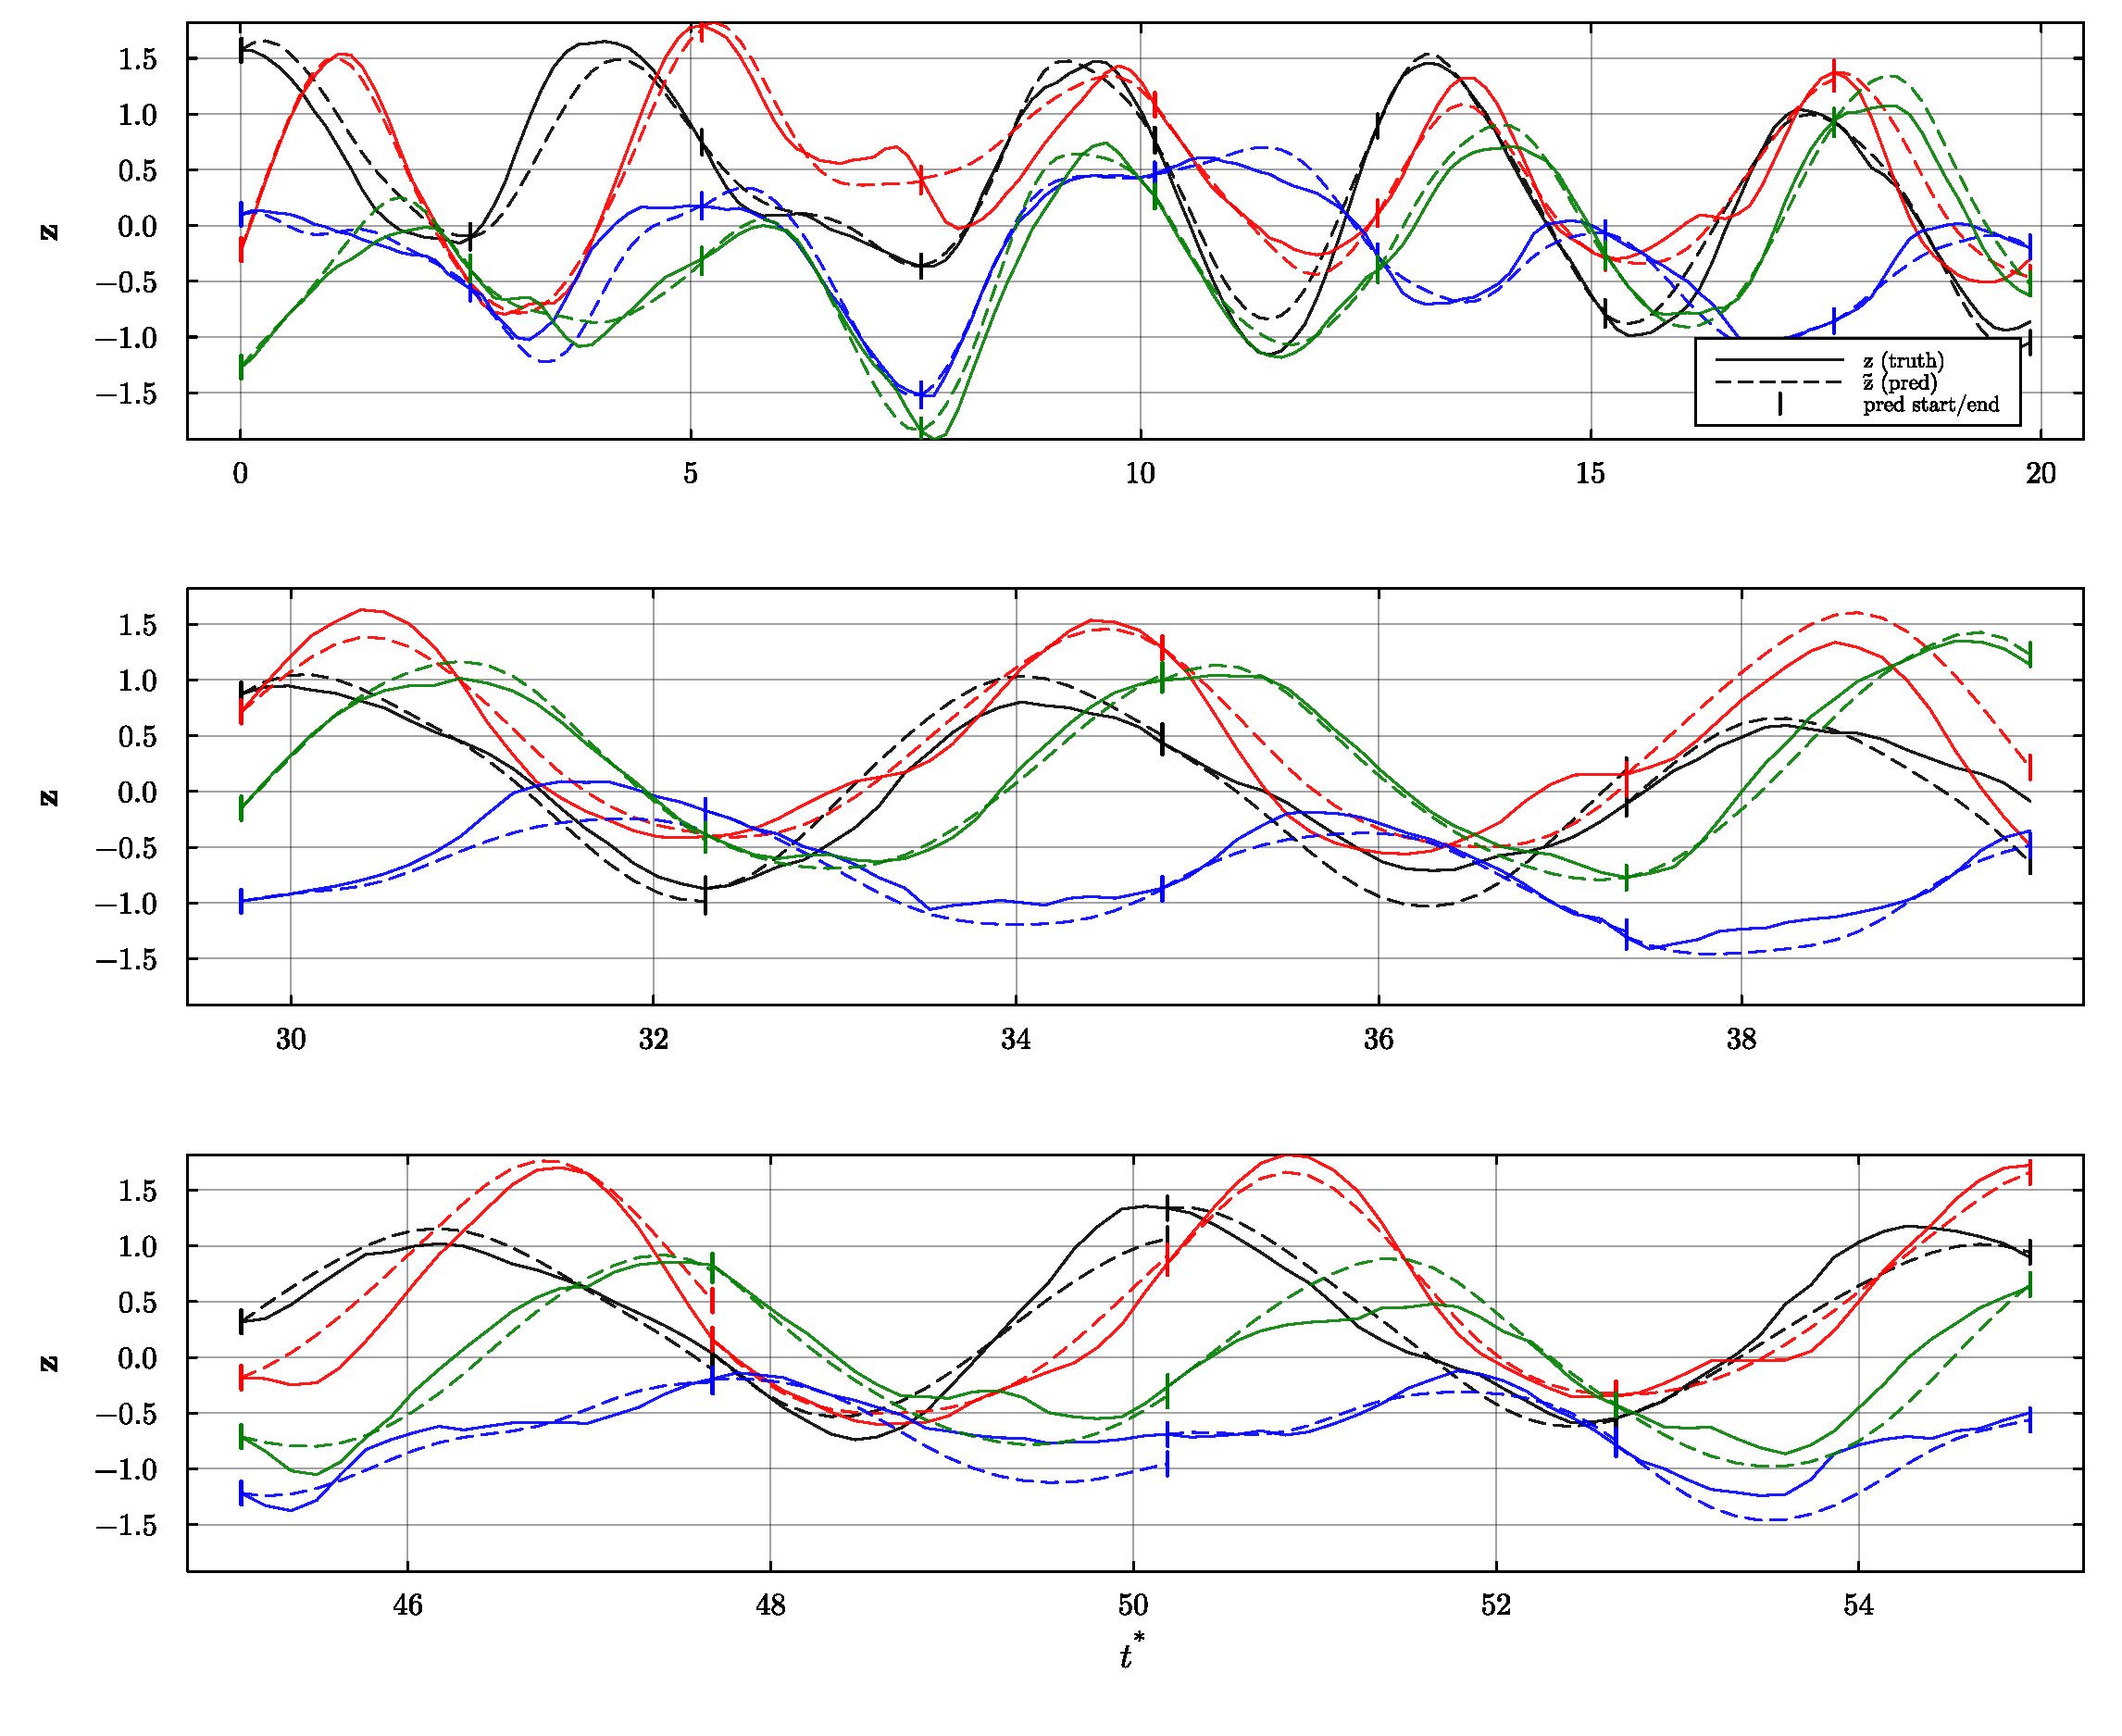
\includegraphics[width=\linewidth]{figures/Results/gs20_trajectories.pdf}
        \caption{}
        \label{fig: gs20_latent}
    \end{subfigure}
\caption{Converged multiple-shooting fits for all training and retraining loops. (a) $n_s = 10$ and (b) $n_s = 20$; reference $z$ (solid) against prediction $\tilde{z}$ (dashed), four representative latent components over the training windows. The smaller group tracks the finer oscillation detail within each segment; the larger group recovers a smoother, lower-fidelity trajectory. Baseline fit is shown in \autoref{fig: retrain2_node_rollout}}    
\label{fig: gs_latents}
\end{figure}


\autoref{fig: gs_latents} shows the converged fits for $n_s=10$ and $n_s=20$. The small group reproduces the finer features of the latent oscillation more tightly within each segment, where the large group fits a smoother trajectory that loses some of the higher-frequency fidelity of the latent trajectory. The tighter fit of the small group lets $f_\phi$ produce in-distribution rollouts for longer at inference: the smallest group $n_s = 10$ sustains the longest unaided rollouts, $948$ steps per prediction, against $686$ for $n_s = 20$ and $408$ for the baseline $n_s = 15$, and correspondingly requires a single parameter update, only switches back to CFD stabilisation $6$ times, against $7$ and $9$. This carries directly into the acceleration of \autoref{fig: gs_speedup}: $n_s = 10$ attains $S_\mathrm{loop} = 1.65$ and $S_\mathrm{eff} = 0.093$, the highest of the three. The dependence on $n_s$ proves to be not strictly monotonic, since the baseline rollouts are on average shorter than those of $n_s = 20$, despite its intermediate group size. The actual optimum for the group size is rather hard to determine with a single run per configuration on a chaotically diverging wake, because of run-to-run variability in when the out-of-distribution monitor first triggers relative to the shedding phase. The advantage of the small group is nonetheless large and consistent across both speedup measures.

\begin{figure}[htp]
  \centering
  \begin{tikzpicture}
    \begin{groupplot}[
        group style={group size=2 by 1, horizontal sep=1.7cm},
        width=6.2cm, height=6.0cm,
        symbolic x coords={10,15,20},
        xtick=data,
        xlabel={$n_s$},
        enlarge x limits=0.30,
        ymajorgrids=true,
        grid style={gray!30},
        nodes near coords,
        every node near coord/.append style={anchor=south, font=\footnotesize},
        tick label style={font=\small},
        label style={font=\small},
        title style={font=\small\bfseries},
      ]
      \nextgroupplot[ybar, bar width=24pt, ylabel={$S_\mathrm{loop}$}, ymin=0, ymax=1.85,
                     title={Inference-loop speedup},
                     nodes near coords={\pgfmathprintnumber[fixed,precision=2]{\pgfplotspointmeta}}]
        % \addplot[draw=black, fill=blue!55] coordinates {(250,2.08) (500,1.48) (750,1.55)};
        \addplot[draw=black, fill=blue!55] coordinates {(10,1.65) (15,1.48) (20,1.32)};
        % \draw[dashed,gray] (axis cs:8,1) -- (axis cs:32,1)
        %   node[pos=0.5,above,font=\scriptsize\itshape,gray,inner sep=1pt]{break-even};
      \nextgroupplot[ybar, bar width=24pt, ylabel={$S_\mathrm{eff}$}, ymin=0, ymax=0.11,
                     ytick={0,0.025,0.05,0.075,0.1,0.125},
                     scaled y ticks=false,
                     yticklabel style={/pgf/number format/fixed, /pgf/number format/precision=3},
                     title={Effective speedup (incl.\ training)},
                     nodes near coords={\pgfmathprintnumber[fixed,precision=3]{\pgfplotspointmeta}}]
        % \addplot[draw=black, fill=orange!75] coordinates {(250,0.111) (500,0.058) (750,0.059)};
        \addplot[draw=black, fill=orange!75] coordinates {(10,0.093) (15,0.073) (20,0.072)};
    \end{groupplot}
  \end{tikzpicture}
  \caption{Effect of multiple shooting group size on hybrid solver acceleration. Left: inference-loop speedup $S_\mathrm{loop}$;  Right: effective speedup $S_\mathrm{eff}$, including training costs.}
  \label{fig: gs_speedup}
\end{figure}


The longer rollouts come at a cost in accuracy, but the full-domain mean-flow and Reynolds-stress statistics are not the relevant measure of that cost here. These fields are accumulated over the entire simulation window, the bulk of which is advanced by the exact solver, so a configuration that produces shorter rollouts spends a larger fraction of its steps in pure CFD and has its field statistics inflated accordingly, independently of how well $f_\phi$ reconstructed the flow during the latent rollouts. Comparing the reconstructed RST and mean-flow fields across group sizes, therefore, rewards the configuration that relied on the surrogate least, rather than the one that reconstructed the flow most faithfully, and this latter configuration is set aside here. The important takeaway from the group size is that a smaller group is generally the more beneficial choice for the framework: by partitioning the trajectory into shorter segments, the optimiser resolves the finer features of the training dynamics within each segment and passes a more faithful representation of those dynamics to $f_\phi$, as seen in the tighter fit of \autoref{fig: gs10_latent}. This better-captured surrogate is what sustains the longest unaided rollouts and the highest speedup of the three configurations, so for the acceleration objective that motivates the framework, the smaller group is preferable, provided its reduced accuracy in the hybrid regions remains acceptable for the application at hand.


\subsection{Integration monitor}
\label{subsect: 4_integration_monitor}

The integration monitor is the only pipeline component that influences the acceleration without itself being a learned feature: it decides at every prediction attempt how far a rollout is allowed to advance before WaterLily stabilises the simulation (\autoref{sect: fallback}). Rollout length is one of the most dominant influences on $S_\text{loop}$, and the monitor precisely terminates a rollout when its score crosses $\tau$ (\autoref{tab: base_rollout_summary}). The threshold quantile $q$ directly determines how strict the threshold is, thereby controlling the maximal rollout length. To investigate its influence, the quantile is varied over $q \in \{0.9,\,0.95,\,0.99\}$. Tightening the gate (lower $q$, and in turn $\tau$) flags the rollout earlier and shortens the average steps-per-prediction; this trades away $S_\text{loop}$ for a stricter guarantee that the decoded state has not drifted far from the training distribution $\boldsymbol{\mathcal{T}}_z$. A less direct effect is that the threshold governs how quickly OOD flags accumulate towards $n_\text{max,\, flags}$, so the monitor also shifts the retraining intervals, thereby affecting the maximal achievable speedup, $S_\text{eff}$.

\subsubsection{Threshold variation}
As desired in the rollout, tightening the KNN quantile results in stricter gating and shorter rollouts. The average rollout length drops from $408$ steps at the base setting ($q=0.999$) to $307$ at $q=0.95$ and $178$ at $q=0.9$, which is exactly what a lower $\tau$ should do: a tighter threshold notices the latent state drifting away from $\boldsymbol{\mathcal{T}}_z$ sooner, so the conventional solver takes back control after less neural ODE steps. \autoref{fig: threshold_speedup} shows how both speedup metrics follow the same increasing path as the rollout length does for a higher quantile setting.

\begin{figure}[htp]
  \centering
  \begin{tikzpicture}
    \begin{groupplot}[
        group style={group size=3 by 1, horizontal sep=1.8cm},
        width=4.7cm, height=6.0cm,
        symbolic x coords={0.9, 0.95, 0.999},
        xtick=data,
        xlabel={$q$},
        enlarge x limits=0.30,
        ymajorgrids=true,
        grid style={gray!30},
        nodes near coords,
        every node near coord/.append style={anchor=south, font=\footnotesize},
        tick label style={font=\small},
        label style={font=\small},
        title style={font=\small\bfseries},
      ]
      \nextgroupplot[ybar, bar width=16pt, ylabel={$S_\mathrm{loop}$}, ymin=0, ymax=1.85,
                     title={Inference-loop speedup},
                     nodes near coords={\pgfmathprintnumber[fixed,precision=2]{\pgfplotspointmeta}}]
        \addplot[draw=black, fill=blue!55] coordinates {(0.9,1.25) (0.95,1.47) (0.999,1.48)};
      \nextgroupplot[ybar, bar width=16pt, ylabel={$S_\mathrm{eff}$}, ymin=0, ymax=0.11,
                     ytick={0,0.025,0.05,0.075,0.1,0.125},
                     scaled y ticks=false,
                     yticklabel style={/pgf/number format/fixed, /pgf/number format/precision=3},
                     title={Effective speedup (incl.\ training)},
                     nodes near coords={\pgfmathprintnumber[fixed,precision=3]{\pgfplotspointmeta}}]
        \addplot[draw=black, fill=orange!75] coordinates {(0.9,0.047) (0.95,0.055) (0.999,0.073)};
      \nextgroupplot[ybar, bar width=16pt, ylabel={$\bar{n}_\mathrm{roll}$}, ymin=0, ymax=480,
                     title={Avg.\ rollout length},
                     nodes near coords={\pgfmathprintnumber[fixed,precision=0]{\pgfplotspointmeta}}]
        % TODO: replace 0.9 and 0.95 with measured averages; 408 is the q=0.99 baseline
        \addplot[draw=black, fill=green!55!black] coordinates {(0.9,178) (0.95,307) (0.999,408)};
    \end{groupplot}
  \end{tikzpicture}
  \caption{Effect of KNN threshold quantile $q$ on hybrid solver acceleration. Left: inference-loop speedup $S_\mathrm{loop}$; middle: effective speedup $S_\mathrm{eff}$, including training costs; right: average rollout length $\bar{n}_\mathrm{roll}$ in CFD steps per accepted prediction.}
  \label{fig: threshold_speedup}
\end{figure}

An important point about the stricter rollout gating is that the monitor at $q=0.9$ triggers one more retraining cycle than the monitors at $q=0.95$ and $q=0.999$, which trigger the same number of retraining cycles. Since training the ML components dominates the wall-time budget, this single extra cycle is what drags $S_\text{eff}$ down to $0.047$, compared with $0.055$ at $q=0.95$ and $0.073$ at $q=0.999$. The smaller gap between the latter two is driven instead by the shorter rollouts at $q=0.95$, which force the conventional solver to do more of the work. A tight KNN threshold, therefore, erodes the achievable acceleration through two channels: shorter rollouts that hand more of the workload back to the slower conventional solver, and more frequent flagging that triggers additional retraining.


\section{Generalisation}
\label{sect: 4_generalization}
The results presented so far were obtained at a single operating point, namely the cylinder wake at $Re = 2500$ on a $256 \times 256$ grid, a regime deliberately chosen to test the limits of the autoencoder and neural ODE under a manageable computational cost. This section steps away from that point to inspect how the achieved acceleration and physical fidelity respond to the two parameters that define the problem, the flow regime and the grid resolution.  The Reynolds number is first reduced to a lower shedding regime to assess the pipeline's behaviour, where the dynamics are simpler and more periodic. Following this, the grid is refined and the Reynolds number is doubled to $Re=5000$ to stress test how the achieved acceleration scales with problem size and how the framework handles more complex flow dynamics. 

Unless stated otherwise, all parameters are kept identical to those of the base case reported in \autoref{sect: 4_setup}; the autoencoder architecture, latent dimension $N_z = 16$, the multiple-shooting settings ($n_s = 15$, $\lambda_c= 200$), and the KNN monitor calibration are left unchanged, so that any difference in the results below is just an effect of the change in flow regime or grid resolution alone.

\subsection{Re 250}
\label{subsect: 4_re250}
At $Re = 250$, the cylinder wake sheds as a clean periodic cycle with a single shedding frequency and less abrupt gradients between flow structures. \autoref{fig: re250_vortex_shedding} displays the vorticity field of the new flow regime in 5 consecutive snapshots. 

\begin{figure}[htbp]
    \centering
    \begin{subfigure}[b]{0.19\textwidth}
        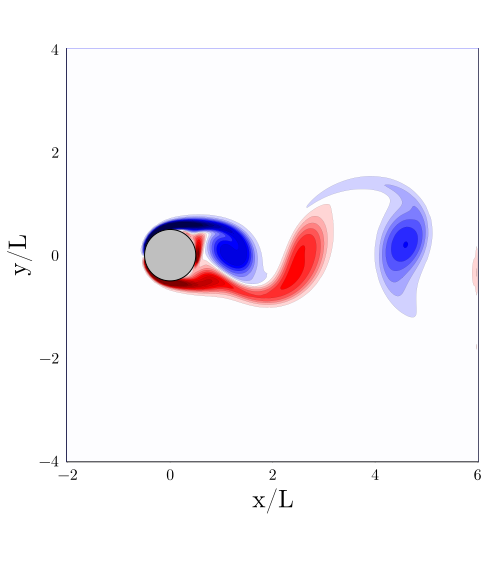
\includegraphics[width=\textwidth]{figures/Results/Re250/vort_snapshots/RE250_shedding_t0.5.png}
        \caption{$t^*_{n}$}
    \end{subfigure}
    \begin{subfigure}[b]{0.19\textwidth}
        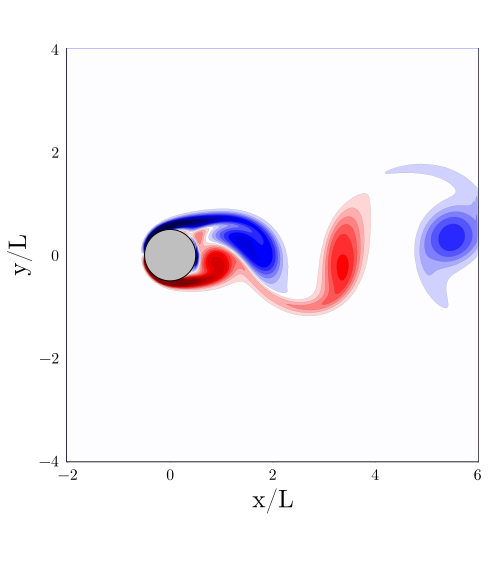
\includegraphics[width=\textwidth]{figures/Results/Re250/vort_snapshots/RE250_shedding_t1.5.png}
        \caption{$t^*_{n+\Delta t}$}
    \end{subfigure}
    \begin{subfigure}[b]{0.19\textwidth}
        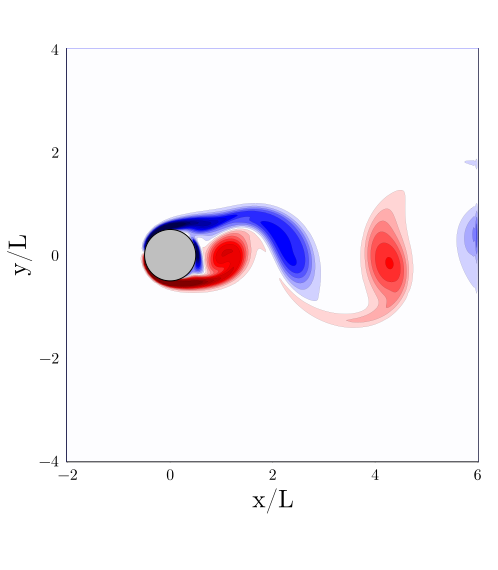
\includegraphics[width=\textwidth]{figures/Results/Re250/vort_snapshots/RE250_shedding_t2.5.png}
        \caption{$t^*_{n+ 2\Delta t}$}
    \end{subfigure}
    \begin{subfigure}[b]{0.19\textwidth}
        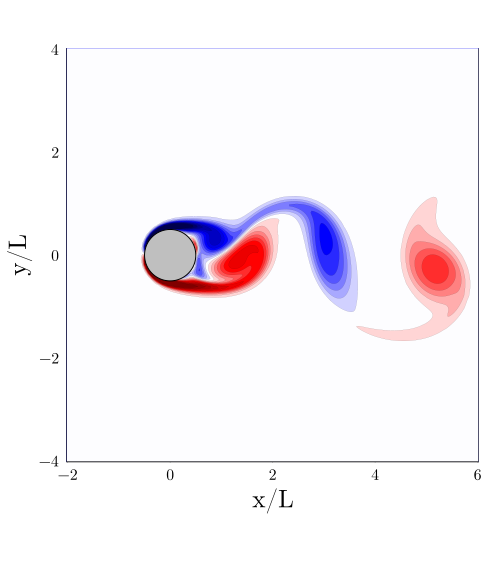
\includegraphics[width=\textwidth]{figures/Results/Re250/vort_snapshots/RE250_shedding_t3.5.png}
        \caption{$t^*_{n+ 3\Delta t}$}
    \end{subfigure}
    \begin{subfigure}[b]{0.19\textwidth}
        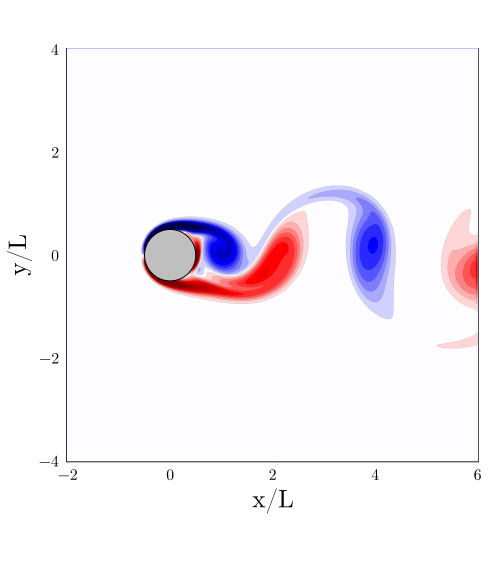
\includegraphics[width=\textwidth]{figures/Results/Re250/vort_snapshots/RE250_shedding_t4.5.png}
        \caption{$t^*_{n+ 4\Delta t}$}
    \end{subfigure}
    \caption{Vorticity field $\omega \nicefrac{L}{U}$ of five consecutive snapshots at $Re=250$. Indicating positive (red) and negative (blue) vorticity. Showing the clean periodic shedding}
    \label{fig: re250_vortex_shedding}
\end{figure}


This new flow regime will prove to be no challenge to $\mathcal{P}$, which is able to capture this regime with high fidelity: the latent dynamics $f_\phi$ are able to track the encoded trajectory $\boldsymbol{\mathcal{T}}_z$ closely throughout the training window. \autoref{fig: Re250_latent_traj} shows the cleanly periodic latent trajectories, the multiple shooting fits and a single training span rollout of the latent dynamics. 

\begin{figure}[H]
    \centering
    \begin{subfigure}[t]{0.48\textwidth}
        \centering
        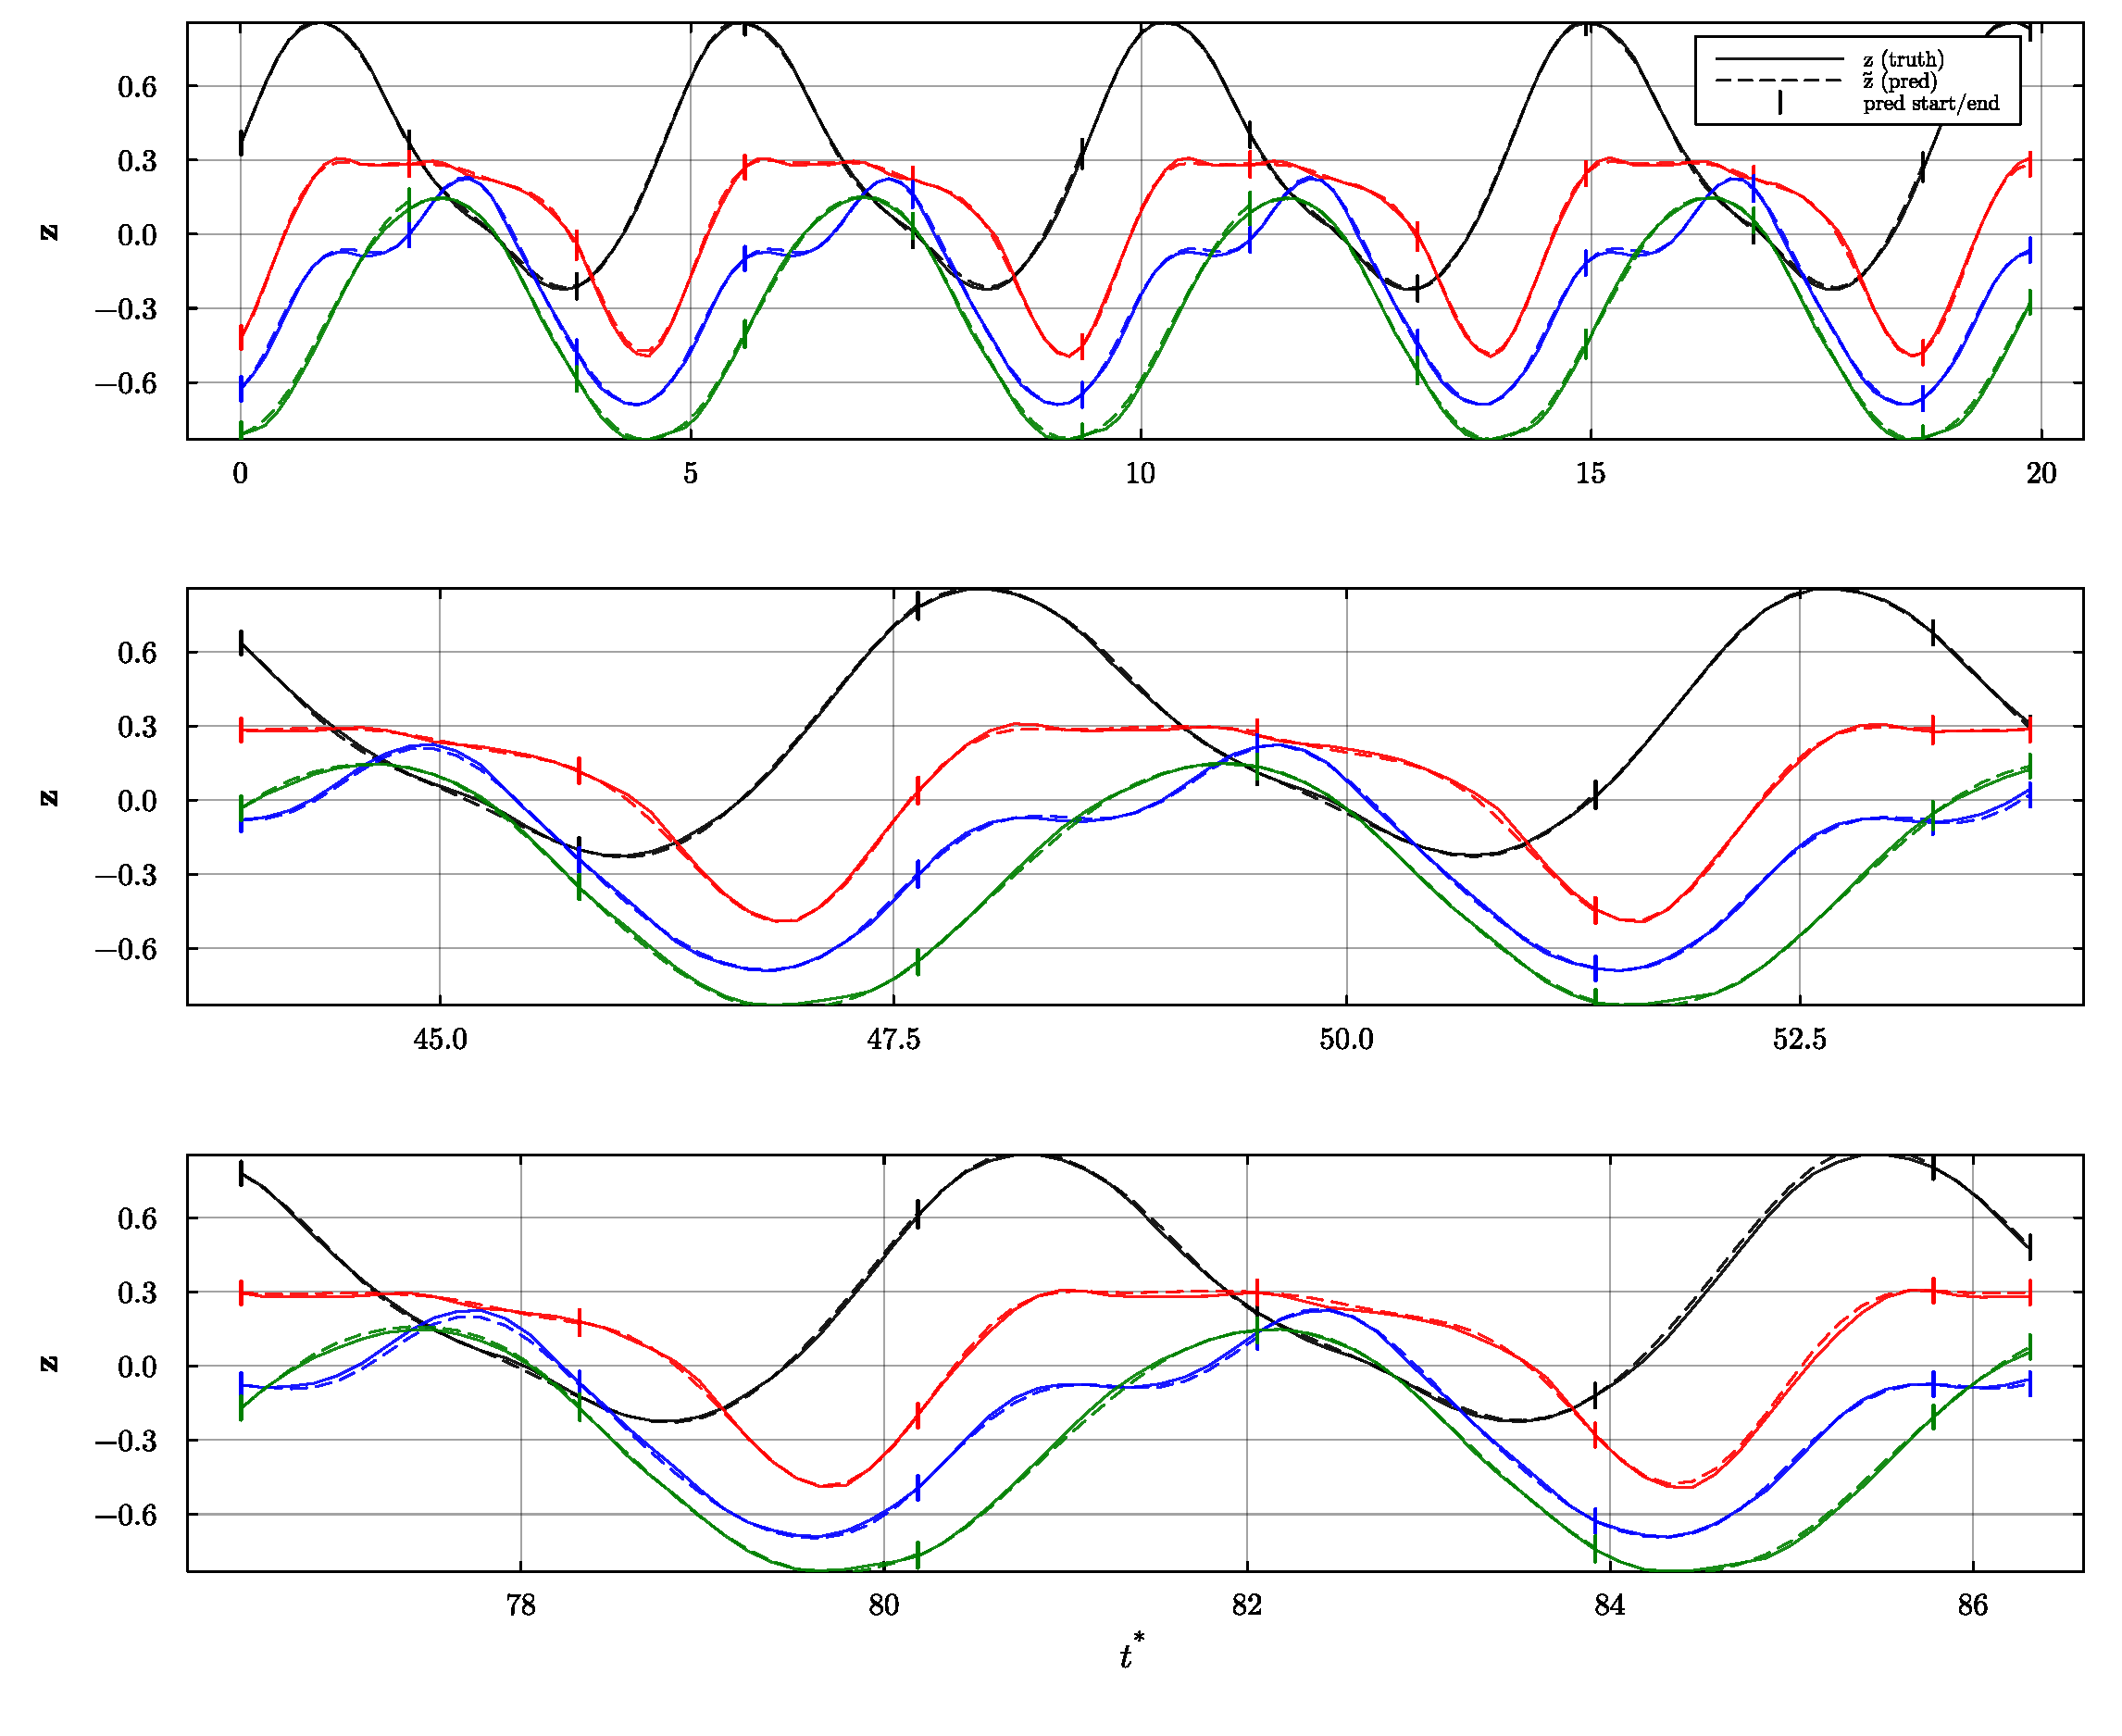
\includegraphics[width=\linewidth]{figures/Results/Re250/trajectories.pdf}
    \caption{Converged multiple-shooting fit on the augmented trajectory set; markers denote shooting-segment boundaries.}
    \label{fig: Re250_retrain_node_ms}
    \end{subfigure}
    \begin{subfigure}[t]{0.48\textwidth}
        \centering
        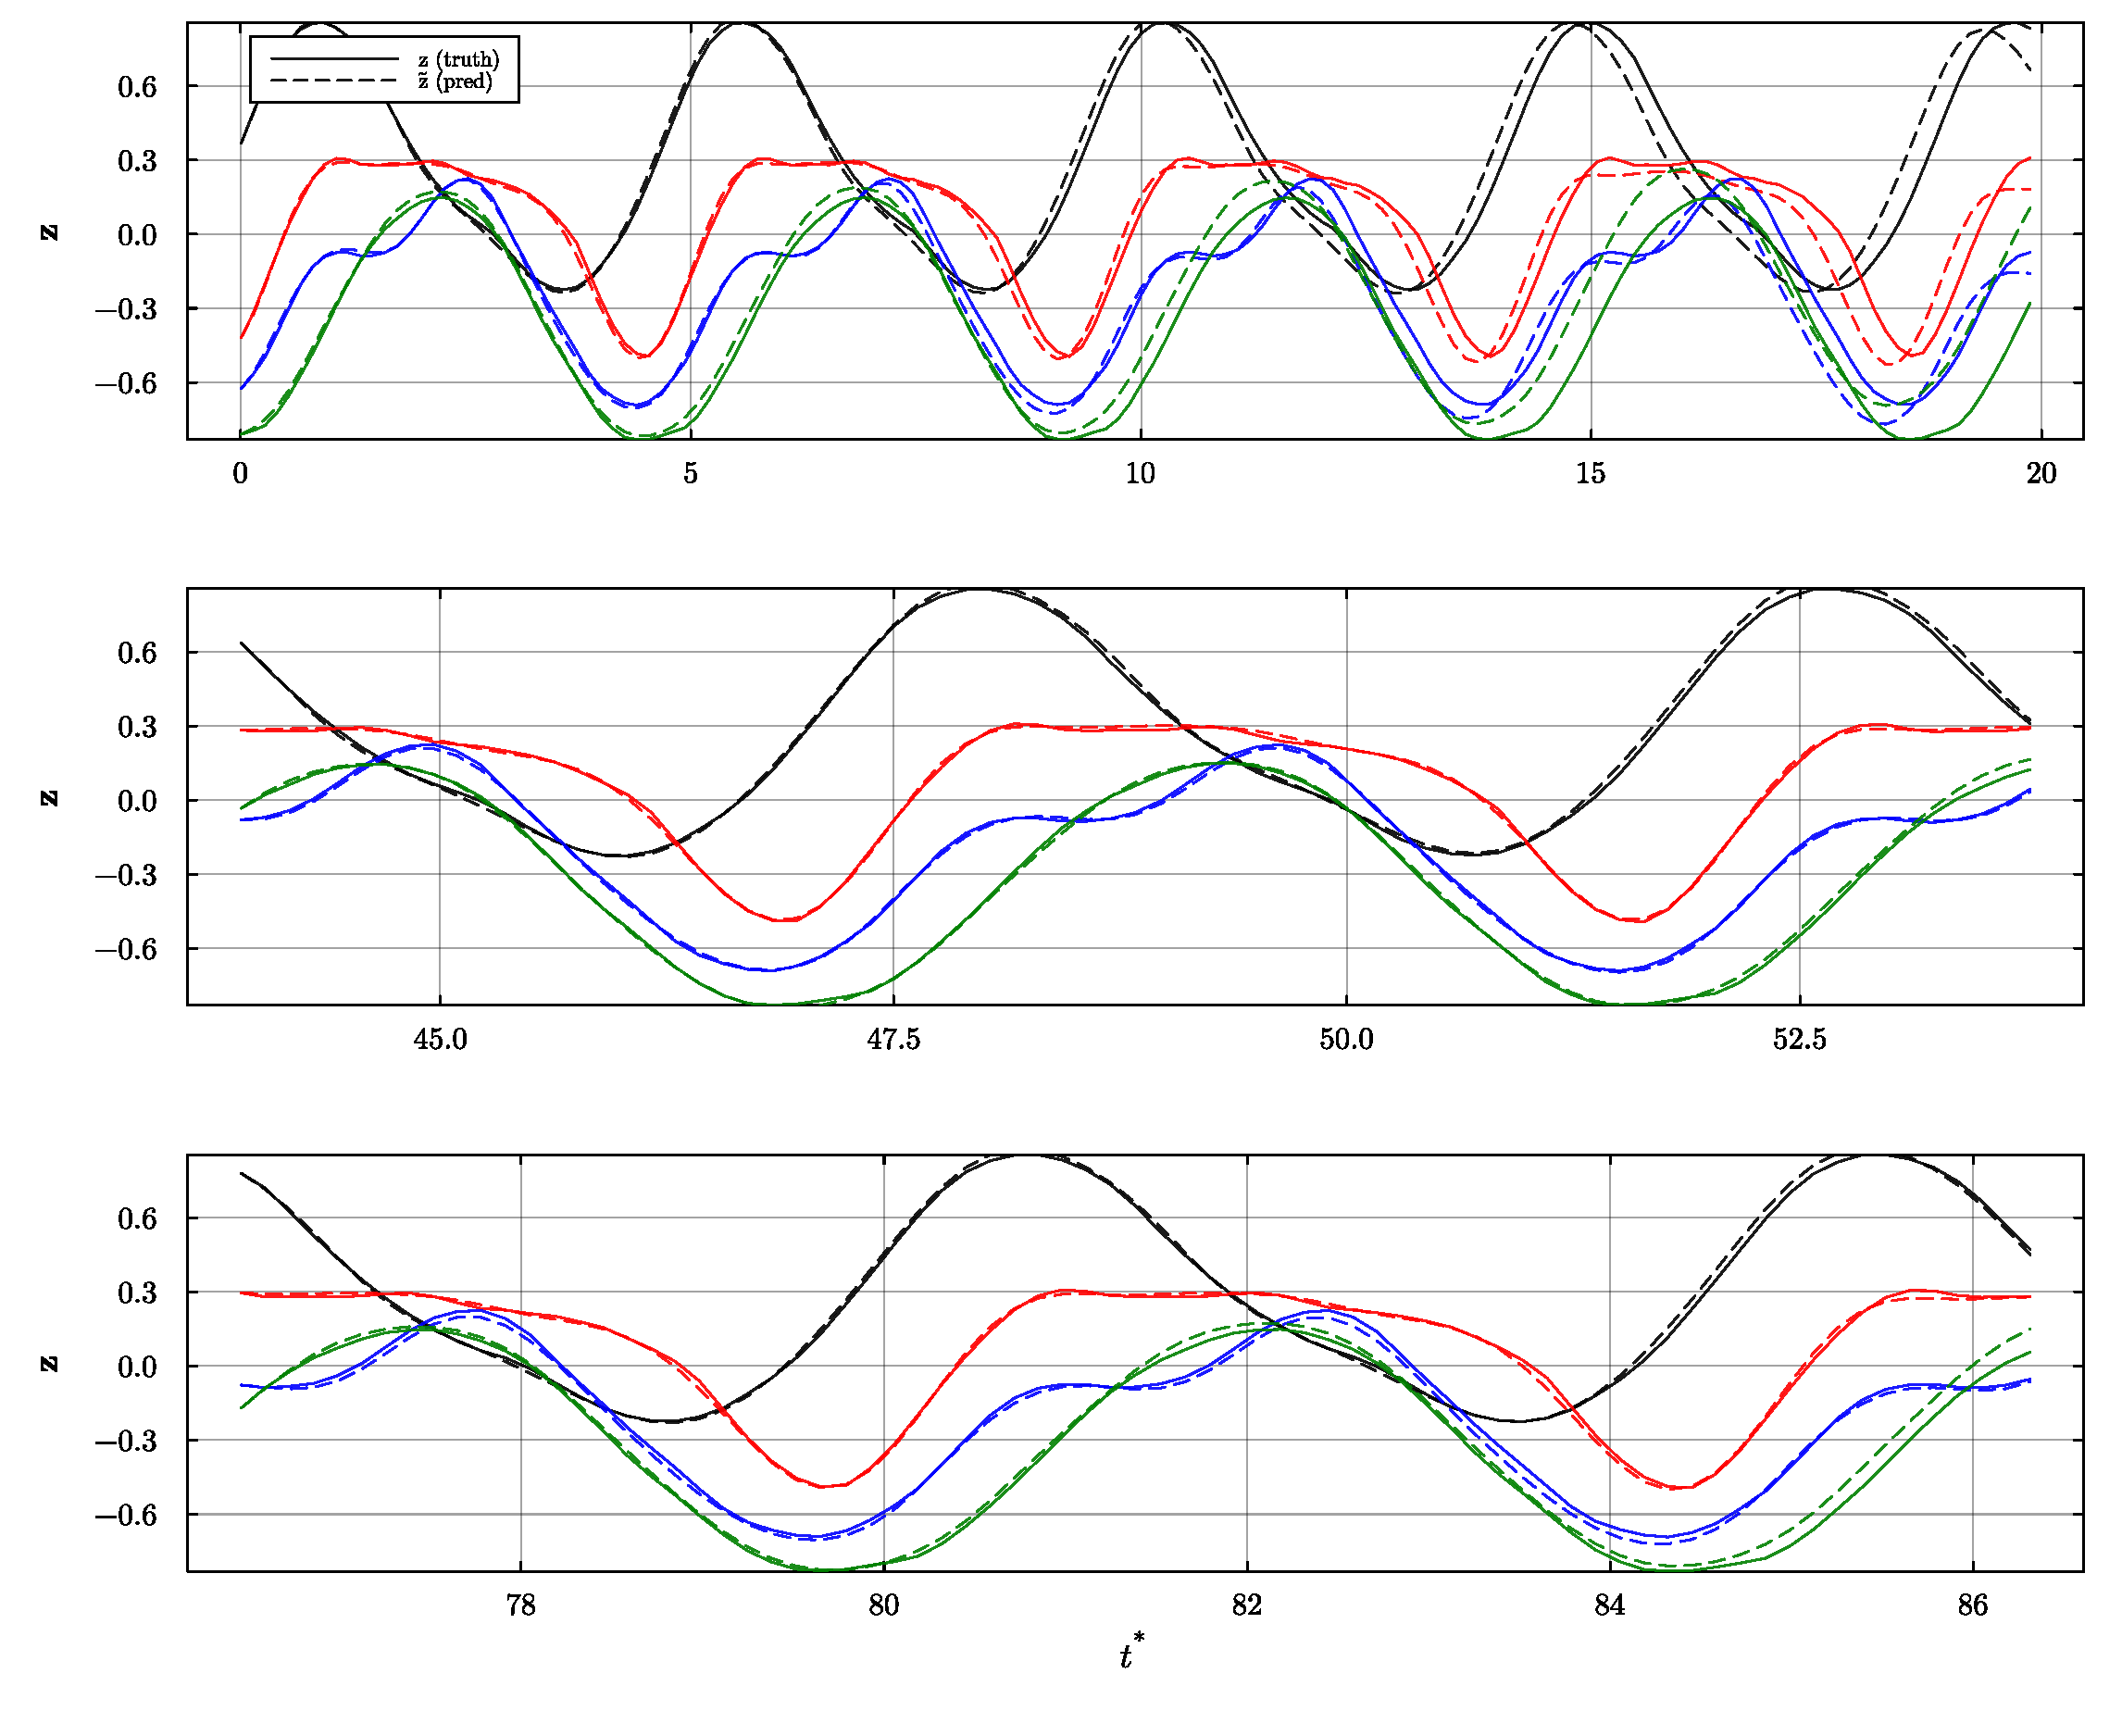
\includegraphics[width=\linewidth]{figures/Results/Re250/rollout_single_shooting.pdf}
    \caption{Single rollout from $t^*=0$ across both windows after the first retraining, no segment resets.}
    \label{fig: Re250_retrain_node_singleshoot}
    \end{subfigure}
    \caption{Latent dynamics of $f_\phi$ at $Re=250$, four representative components shown over all time windows. Reference $z$ (solid) against prediction $\tilde{z}$ (dashed). (a) Converged multiple-shooting fit on the augmented trajectory set, with segment start/end markers; (b) unaided single rollout from $t^*=0$ over the same windows.}
    \label{fig: Re250_latent_traj}
\end{figure}

This high-quality fit, however, is double-edged. Because of the periodic nature of the wake, the latent vectors will form a low variance distribution in the $N_z$ dimensional space. Meaning that the distances between each latent vector follow this distribution tightly. So the neighbour distances on which the KNN monitor $\mathcal{K}$ is calibrated are small, and the resulting threshold $\tau$ will be overly tight and allow almost no drift of the neural ODE. This behaviour is confirmed in \autoref{fig: RE250_forces} together with \autoref{tab: re250_rollout_summary}.

\begin{figure}[htbp]
  \centering
  % ---- left: image ----
  \begin{minipage}[c]{0.46\textwidth}
    \centering
    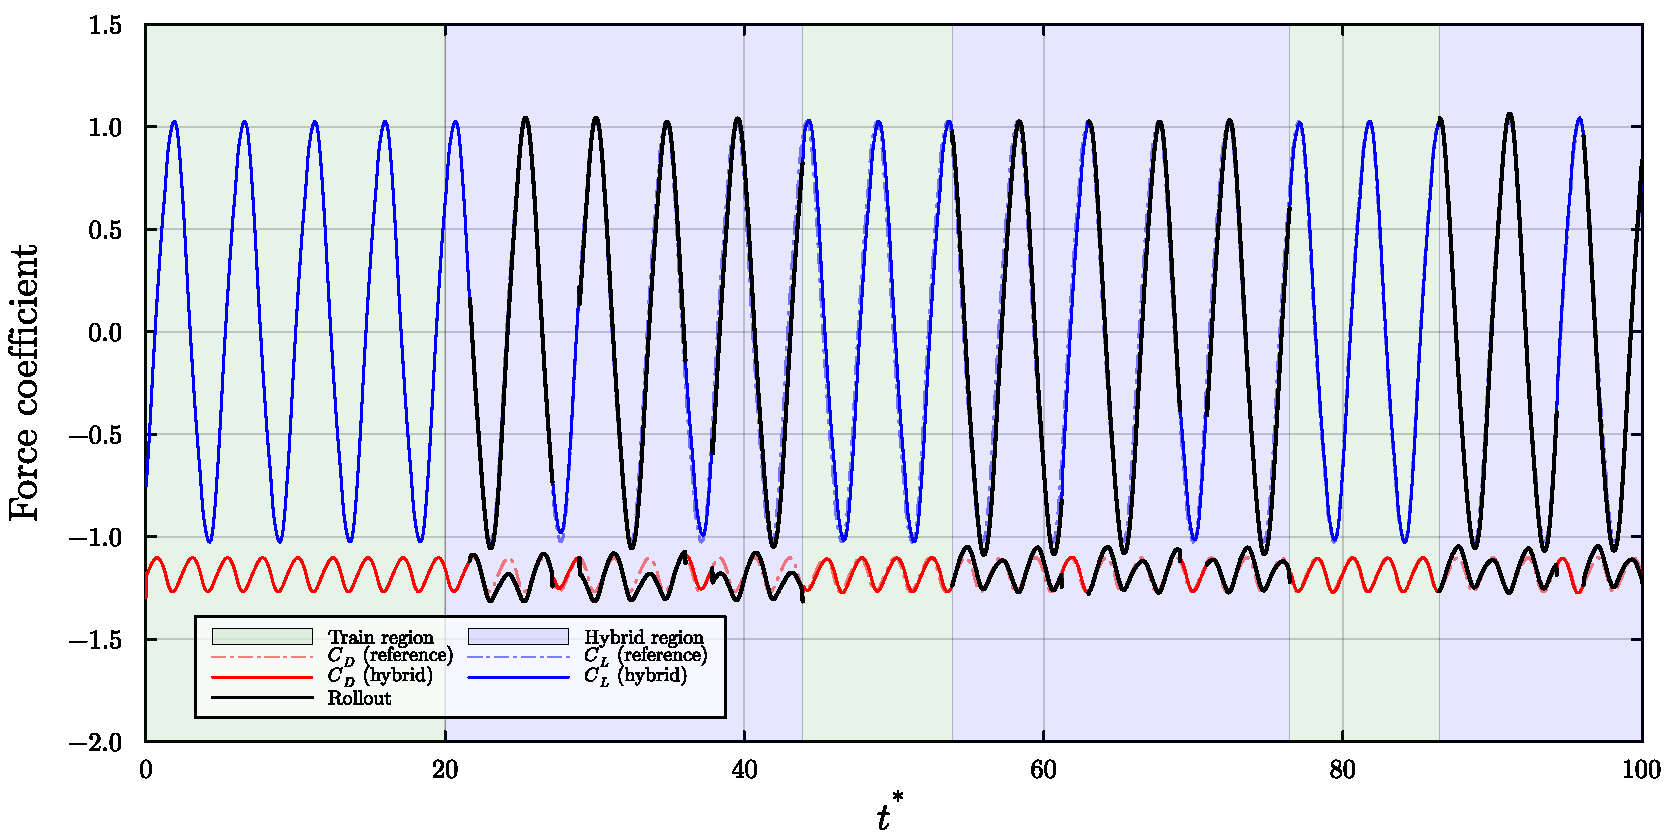
\includegraphics[width=\linewidth]{figures/Results/Re250/plt_forces.pdf}
    \caption{Force coefficients comparison for the $Re = 250$ hybrid run. Showing that the simpler wake dynamics are quickly learnt, but longer rollouts are prevented by a strict KNN threshold.}
    \label{fig: RE250_forces}
    % \vspace{2em}
  \end{minipage}\hfill
  % ---- right: table ----
  \begin{minipage}[c]{0.52\textwidth}
    \centering
    \footnotesize
    \setlength{\tabcolsep}{4pt}
    \renewcommand{\arraystretch}{0.85}
    \begin{tabular}{clrrrcc}
      \toprule
      \# & NODE model & Steps & $\Delta t^*$ & $t^*_\text{r, end}$ & score & $\tau$ \\
      \midrule
      1 & initial      & 505 & 5.516  & 27.176  & 0.0753 & 0.0720 \\
      2 & initial      & 647 & 8.889  & 36.065  & 0.0722 & 0.0720 \\
      3 & initial      & 550 & 7.825  & 43.890  & 0.0749 & 0.0720 \\
      \midrule
      4 & 1st retrain  & 667 & 17.319 & 61.209  & 0.0657 & 0.0654 \\
      5 & 1st retrain  & 558 & 7.909  & 69.118  & 0.0682 & 0.0654 \\
      6 & 1st retrain  & 505 & 7.327  & 76.445  & 0.0657 & 0.0654 \\
      \midrule
      7 & 2nd retrain  & 716 & 17.847 & 94.292  & 0.0741 & 0.0736 \\
      8 & 2nd retrain  & 358 & 5.724  & 100.017 & --     & 0.0736 \\
      \bottomrule
    \end{tabular}
    \captionof{table}{Per-rollout summary of the KNN-gated NODE inference at $Re = 250$. Every accepted rollout terminates marginally above the active threshold $\tau$; rollout~8 is capped by the $t^* = 100$ cutoff while still in distribution.}
    \label{tab: re250_rollout_summary}
  \end{minipage}
\end{figure}


\autoref{fig: RE250_forces} does show that $\psi_\theta$ is able to reconstruct the gradients close to the cylinder wall rather well. Since the force coefficients match exactly those of the reference simulation. Showing that for this reduced Reynolds number, the relevant velocity gradients are less harsh, and can thus be reconstructed rather well compared to the higher Reynolds number contour plots seen in \autoref{fig: base_curl_comp}.


When analysing the inference-loop speedup over the complete simulation window $t^* \in [0, 100]$ is
%
\begin{align}
  S_\text{loop} = \frac{T_\text{wall}^\text{ref}}{T_\text{wall}^\text{h, tot}}
  = \frac{\SI{114.41}{\second}}{\SI{62.50}{\second}} = 1.83,
\end{align}
%
with the hybrid total splitting into $T_\text{wall}^\text{h, cfd} \approx \SI{61.50}{\second}$ of stabilising CFD steps and $T_\text{wall}^\text{h, rollout} = \SI{1.00}{\second}$ for the eight accepted latent rollouts of \autoref{tab: re250_rollout_summary}. The rollouts themselves make up only $1.6\%$ of the loop wall time; the denominator is almost entirely WaterLily CFD steps. Just as in the base simulation, $\mathcal{P}$ proves to be an order of magnitude faster per unit simulated time than the solver it replaces, but the tight OOD gate forces roughly half of the simulation window to be covered by CFD steps between rollouts, diluting the realised $S_\text{loop}$ to $1.83$. The acceleration potential of the simpler $Re = 250$ dynamics is real but largely unrealised, gated by rollout length rather than by the cost of the latent dynamics $f_\phi$. 

When adding the training cost of the networks, the effective speedup of the complete workflow can be realised.
%
\begin{align}
  S_\text{eff}
  = \frac{T_\text{wall}^\text{ref}}{T_\text{wall}^\text{h, tot} + T_\text{wall}^\text{h, training}}
  = \frac{\SI{114.41}{\second}}{\SI{62.50}{\second} + \SI{1266}{\second}} \approx 0.086,
\end{align}
%
where the training wall time cost $T_\text{wall}^\text{h, training} = \SI{21.1}{\minute}$ covers the initial autoencoder and NODE training and the two retrain phases. As in the base case, the workflow is much slower than plain WaterLily once training is included in the speedup factor, since the training costs still dwarf the short reference run. The effective speedup is comparable to that of the base case, because the autoencoder dominates the training budget and takes a similar amount of wall time in both regimes.

% \todo{conclude}

% -----------------------------------------------------------------------------------------------
\subsection{Re 5000}
\label{subsect: 4_RE5000}

As established in \autoref{subsect: 4_wall_time}, the per-CTU advantage of the latent rollout is tied to the base-case resolution: since the WaterLily solver is memory-bound, its cost per CTU grows with the grid size~\cite{Weymouth2025}, whereas a single rollout of $\mathcal{P}$ is fixed by the latent dimension $N_z = 16$ and is independent of the grid. The $256^2$ baseline used throughout this work is therefore a comparatively inexpensive and dynamically simple case for demonstrating the gain. To assess the hybrid loop on a simultaneously more expensive and more demanding regime, the reference case is re-run with an increase in Reynolds number to $Re = 5000$ and the grid refined to $512^2$, keeping the domain and cylinder geometry of \autoref{tab: parameters} fixed. These two changes act on different parts of the framework. The finer grid raises the cost per CTU of the reference solver while leaving the rollout cost untouched, which should widen the achievable acceleration margin, whereas the higher Reynolds number drives the wake from the quasi-periodic shedding of the baseline towards a more complex shedding state with sharper near-body shear layers and more complex structures in the wake, as displayed in \autoref{fig: RE5000_vortex_shedding}. 

% The following paragraphs quantify both effects in turn: how the combined refinement shifts the cost per CTU and the resulting upper bound on the speedup, and how the more chaotic wake stresses the reconstruction and the integrated force statistics on which the hybrid loop is assessed.


\begin{figure}[htbp]
    \centering
    \begin{subfigure}[b]{0.19\textwidth}
        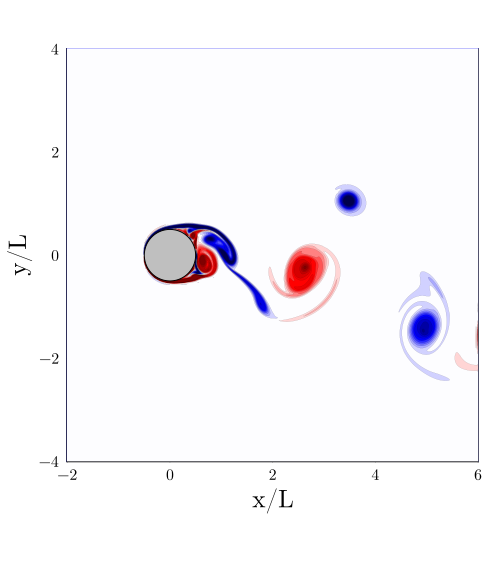
\includegraphics[width=\textwidth]{figures/Results/RE5000/cover/vorticity_t000.50.png}
        \caption{$t^*_{n}$}
    \end{subfigure}
    \begin{subfigure}[b]{0.19\textwidth}
        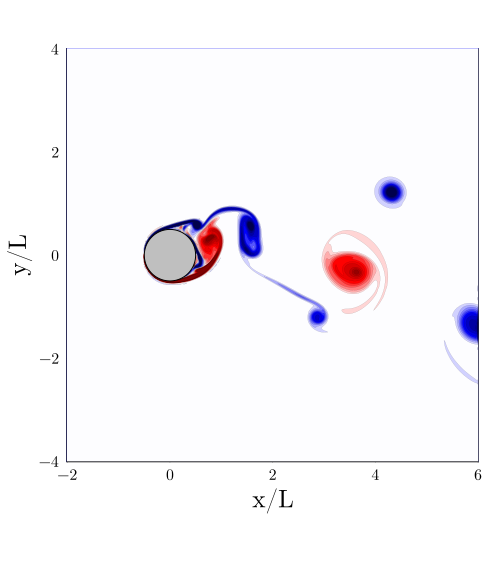
\includegraphics[width=\textwidth]{figures/Results/RE5000/cover/vorticity_t001.50.png}
        \caption{$t^*_{n+\Delta t}$}
    \end{subfigure}
    \begin{subfigure}[b]{0.19\textwidth}
        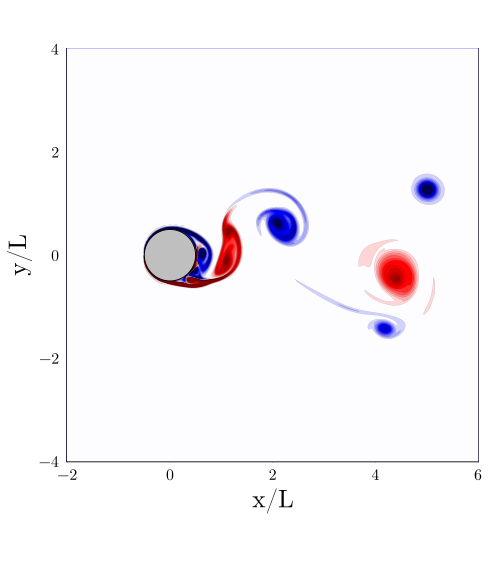
\includegraphics[width=\textwidth]{figures/Results/RE5000/cover/vorticity_t002.50.png}
        \caption{$t^*_{n+ 2\Delta t}$}
    \end{subfigure}
    \begin{subfigure}[b]{0.19\textwidth}
        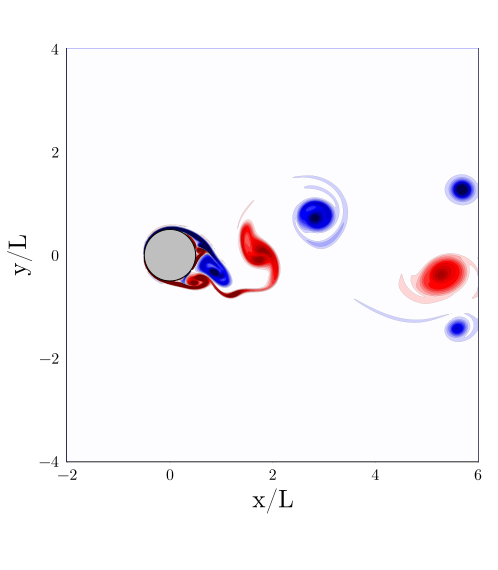
\includegraphics[width=\textwidth]{figures/Results/RE5000/cover/vorticity_t003.50.png}
        \caption{$t^*_{n+ 3\Delta t}$}
    \end{subfigure}
    \begin{subfigure}[b]{0.19\textwidth}
        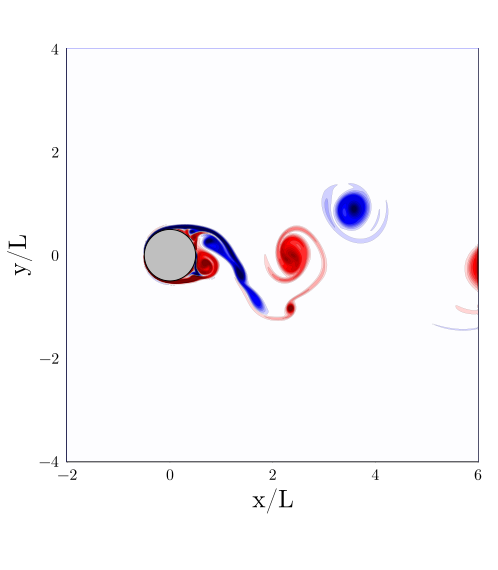
\includegraphics[width=\textwidth]{figures/Results/RE5000/cover/vorticity_t004.50.png}
        \caption{$t^*_{n+ 4\Delta t}$}
    \end{subfigure}
    \caption{Vorticity field $\omega \nicefrac{L}{U}$ of five consecutive snapshots at $Re=5000$. Indicating positive (red) and negative (blue) vorticity. The refined grid and higher Reynolds number result in more complex wake structures that are more sharply resolved than those of the $256^2$ baseline.}
    \label{fig: RE5000_vortex_shedding}
\end{figure}

\subsubsection{Wall time performance}

Following the wall-clock breakdown in \autoref{subsect: 4_wall_time}, the $Re=5000$ hybrid simulation is broken down into its segments, whose wall times are presented in \autoref{tab: wall_timing_hybrid_re5000}. Just as in the base simulation, the initial autoencoder training consumes a very high fraction of $\mathcal{S}$'s total wall time, just over $50\%$ of the total, and once the two retraining cycles are added, building and updating the networks accounts for close to $90\%$ of the $3217$~s pipeline. The initial data-gathering, the initial data-gathering, and the three snapshot-gathering runs make up most of what remains, while the latent rollouts themselves contribute well under $1\%$; the only non-negligible inference-loop cost is the single extended CFD stretch in the second hybrid section (\SI{92.3}{\second}), where the OOD monitor held control with the solver rather than the rollout.

\begin{table}[htbp]
    \centering
    \begin{tabular}{llrr}
        \toprule
        Phase & Component & Time (s) & \% of total \\
        \midrule
        Initial data-gathering & -- & 84.77 & 2.64 \\
        \midrule
        \multirow{2}{*}{Train} & AE   & 1662.00 & 51.66 \\
                               & NODE &  222.00 &  6.90 \\
        \midrule
        \multirow{3}{*}{Hybrid section 1} & CFD + rollout & 3.781 & 0.12 \\
                                          & CFD + rollout & 4.066 & 0.13 \\
                                          & CFD + rollout & 3.986 & 0.12 \\
        \midrule
        \multirow{3}{*}{Retrain 1} & Gather snapshots &  52.57 &  1.63 \\
                                   & AE               & 348.00 & 10.82 \\
                                   & NODE             & 156.00 &  4.85 \\
        \midrule
        \multirow{3}{*}{Hybrid section 2} & CFD + rollout & 0.038 & 0.00 \\
                                          & CFD + rollout & 3.959 & 0.12 \\
                                          & CFD + rollout & 4.776 & 0.15 \\
        \midrule
        \multirow{3}{*}{Retrain 2} & Gather snapshots &  50.30 &  1.56 \\
                                   & AE               & 390.00 & 12.12 \\
                                   & NODE             & 192.00 &  5.97 \\
        \midrule
        \multirow{3}{*}{Hybrid section 3} & CFD + rollout & 0.148 & 0.00 \\
                                          & CFD + rollout & 4.223 & 0.13 \\
                                          & CFD + rollout & 5.002 & 0.16 \\
        \midrule
        Retrain 3 & Gather snapshots & 29.69 & 0.92 \\
        \midrule
        \textbf{Total} & & \textbf{3217.31} & \textbf{100.00} \\
        \bottomrule
    \end{tabular}
    \caption{Wall-clock breakdown of the hybrid simulation pipeline ($Re=5000$ run).}
    \label{tab: wall_timing_hybrid_re5000}
\end{table}


As mentioned, the rollout cost barely changes with the grid. It is fixed by the latent dimension $N_z = 16$ and stays around $48$~ms/CTU, the same order as the base run, because it never touches the full field. The WaterLily time integrations, on the other hand, now cost $4842$~ms/CTU, against $866$~ms/CTU at $256^2$. This large cost difference between rollout and CFD is even more noticeable when inspecting the acceleration metrics, $S_\text{loop}$: 


\begin{align}
  S_\text{loop} = \frac{T_\text{wall}^\text{ref}}{T_\text{wall}^\text{h, tot}}
  = \frac{\SI{651.83}{\second}}{\SI{314.94}{\second}} = 2.07,
\end{align}

Showing that the hybrid loop uses the low-cost rollouts to its full effect, where it is able to achieve a $2.07$ speedup compared to the reference simulation. To assess the speedup of the hybrid loop compared to the training cost of the ML components of $\mathcal{P}$, the training wall time is added to the comparison in $S_\text{eff}$ with $T_\text{wall}^\text{h, training} = 3042$~s of training.


\begin{align}
  S_\text{eff}
  = \frac{T_\text{wall}^\text{ref}}{T_\text{wall}^\text{h, tot} + T_\text{wall}^\text{h, training}}
  = \frac{\SI{651.83}{\second}}{\SI{314.94}{\second} + \SI{3042}{\second}} \approx 0.19,
\end{align}

A single finer run is therefore still much slower than simply running $\mathcal{S}_\text{ref}$, because the training cost is not repaid within one simulation window. But it still performs better than the base case, which achieved an effective speedup of $0.073$, indicating that refining the grid begins to close part of the gap between the full pipeline and running the reference simulation. 

At a lower resolution, this demonstrates that the cost of the framework is dominated by one-off training rather than by the accelerated integration: the inference loop is already cheaper than the reference, and the more expensive the reference, the larger that margin becomes. Closing the remaining gap to break-even no longer requires a faster rollout; it requires either reusing the trained $\mathcal{P}$ across runs or overlapping training with the live simulation, together with a less strict integration monitor to convert the available loop speedup into realised wall-time savings.

\subsubsection{Spatial and physical fidelity}
The finer simulation is passed to $\mathcal{P}$ without any architectural change: the architectures of $\varphi_\theta$, $\psi_\theta$ and $f_\phi$ of \autoref{sect: 4_base_hybrid} are reused as-is. The only change to the architecture is the input and output dimensions of the autoencoder, so that they can correctly pass the new, finer grid down to the latent space without dimension mismatches. An advantage of the grid refinement is that the decoder's fixed cell-width smoothing now spans half the physical width, compared to the base architecture. This means that the thin separating shear layers that dominated the base-grid reconstruction error (\autoref{fig: base_velocity_comp}) are resolved by roughly twice as many cells and blurred less in physical space. Because the autoencoder can now capture finer dynamics to a much greater degree, the cost function converges much faster on the validation set, as displayed in \autoref{fig: RE5000_loss}


\begin{figure}[htbp]
    \centering
    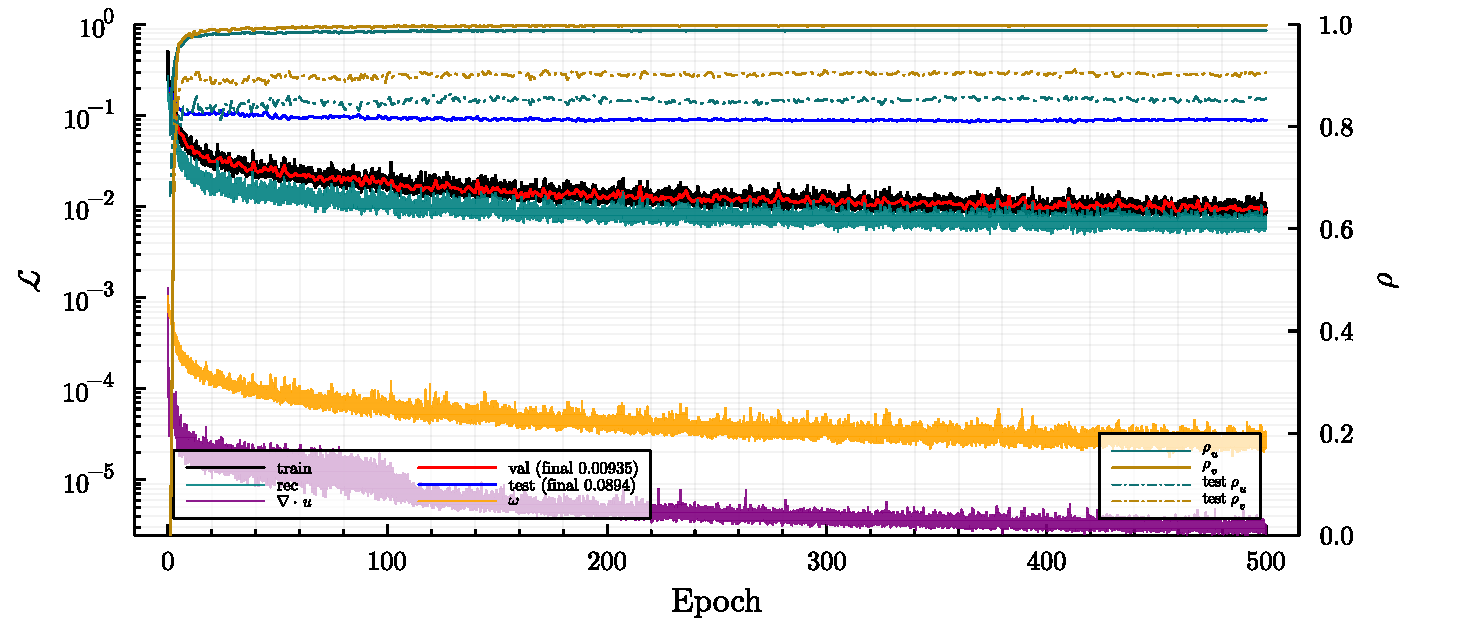
\includegraphics[width=\linewidth]{figures/Results/RE5000/loss_evolution.pdf}
\caption{Initial training history of the autoencoder at the $Re=5000$, $512^2$ operating point. Left axis ($\mathcal{L}$, logarithmic): total loss on the train, validation and test splits, together with the divergence ($\nabla\!\cdot\mathbf{u}$) and vorticity ($\omega$) penalties evaluated on the test split. Right axis ($\rho$): reconstruction correlation coefficients $\rho_u$, $\rho_v$ on train and test. The validation and test losses converge to  $9.6\times10^{-3}$ and $8.9\times10^{-2}$ respectively, the persistent gap between them marking the autoencoder's failure to generalise to the more chaotic wake.}
\label{fig: RE5000_loss}
\end{figure}

% $8.6\times10^{-3}$ and $1.2\times10^{-2}$.}

Comparing the first autoencoder training to that of the base case in \autoref{fig: initial_training_base}, the AE is able to achieve a lower loss on the train and validation set, but the poor performance of the test set proves that the more chaotic wake, due to the increased Reynolds number, is not captured by the train/validation window alone. The gap between the converged train/validation loss and the test loss is markedly wider than the factor of two seen at base resolution, indicating that the held-out window $t^*\in[17.5,\,20]$ contains wake states the autoencoder has not encountered during training. Whereas the base-case wake repeats structures that the network has already learnt, the $Re=5000$ test split presents the autoencoder with spatial configurations not represented in the earlier shedding cycles, so $\varphi_\theta$ and $\psi_\theta$ generalise poorly beyond the training horizon despite the lower in-sample loss. The lower train/validation loss is therefore not evidence of a better fit but of a wake whose aperiodicity the four training cycles cannot span: the autoencoder reconstructs what it has seen more tightly, yet fails to extrapolate to unseen states, which, for a wake this chaotic, makes generalisation intrinsically harder.

However, \autoref{fig: RE5000_loss} shows that the early plateau of the autoencoder training shows that a large part of the training budget is spent unnecessarily. Unlike the base case, the test loss barely changes over the performed epochs; it settles at its higher level within the first $\sim\!100$ epochs and does not improve thereafter, so the remaining epochs only tighten the in-sample fit without recovering any accuracy on the held-out window. Because the generalisation performance at this Reynolds number is set by the spatial information contained in the training set rather than by the length of training, the epochs spent past the plateau buy nothing on the unseen wake states and can be removed at no cost to the test-set reconstruction. Since the initial autoencoder consumes just over half of the workflow budget (\autoref{tab: wall_timing_hybrid_re5000}), early-stopping it at the convergence knee, together with the same reduction applied to the two retraining cycles, translates directly into a higher effective speedup. If the initial autoencoder were trained for only $\sim\!100$ epochs, and the retraining runs cut to the same fraction, the complete training time would fall from \SI{3042}{\second} to roughly \SI{1100}{\second} while leaving the reconstruction accuracy unchanged, since that accuracy was already reached at the plateau. This yields a projected effective speedup of:

\begin{align}
  S_\text{eff}
  = \frac{T_\text{wall}^\text{ref}}{T_\text{wall}^\text{h, tot} + T_\text{wall}^\text{h, training}}
  = \frac{\SI{651.83}{\second}}{\SI{314.94}{\second} + \SI{1100}{\second}} \approx 0.46,
\end{align}

This speedup value shows that trimming the autoencoder training schedule alone moves $S_\text{eff}$ from $0.19$ using the initial training scheme to $0.46$, an order-of-magnitude gain that moves the integrated workflow from roughly ten times slower than the reference to within a factor of two of break-even, without touching the inference loop itself. It demonstrates that the cost of the framework is dominated by one-off training rather than by the accelerated integration: the inference loop is already cheaper than the reference, and the finer the grid, the larger that margin becomes. A single from-scratch run does not yet break even, but closing the remaining gap no longer requires a faster rollout; it requires either better use of the trained $\mathcal{P}$ across runs or overlapping training with the live simulation, together with a less strict integration monitor and switching schedule to convert the available loop speedup into actual wall-time savings

However, it is important to stress that this trimming does not improve the physical fidelity of the run; the generalisation gap and the force errors it produces are unchanged. The speedup is recovered by stopping at the same accuracy sooner, not by reaching a better one.


As the generalisation gap in \autoref{fig: RE5000_loss} indicates, $\mathcal{P}$ will not generalise well outside of the training set, because the test loss of the AE sets the ceiling of the achievable accuracy of the acceleration framework. Where this becomes physically visible is the loading on the cylinder: a faithful velocity reconstruction is the prerequisite for the hybrid loop to reproduce the forces accurately, since the coefficients are computed from the decoded velocity $\hat{\mathbf{u}}$, so the near-body reconstruction error feeds directly into the pressure projection and the integrated force. At $Re=5000$ this reconstruction is no longer faithful, and the consequence is shown in \autoref{fig: RE5000_forces}, where the hybrid force coefficients are compared against the reference over the simulation window.

\begin{figure}[htbp]
    \centering
    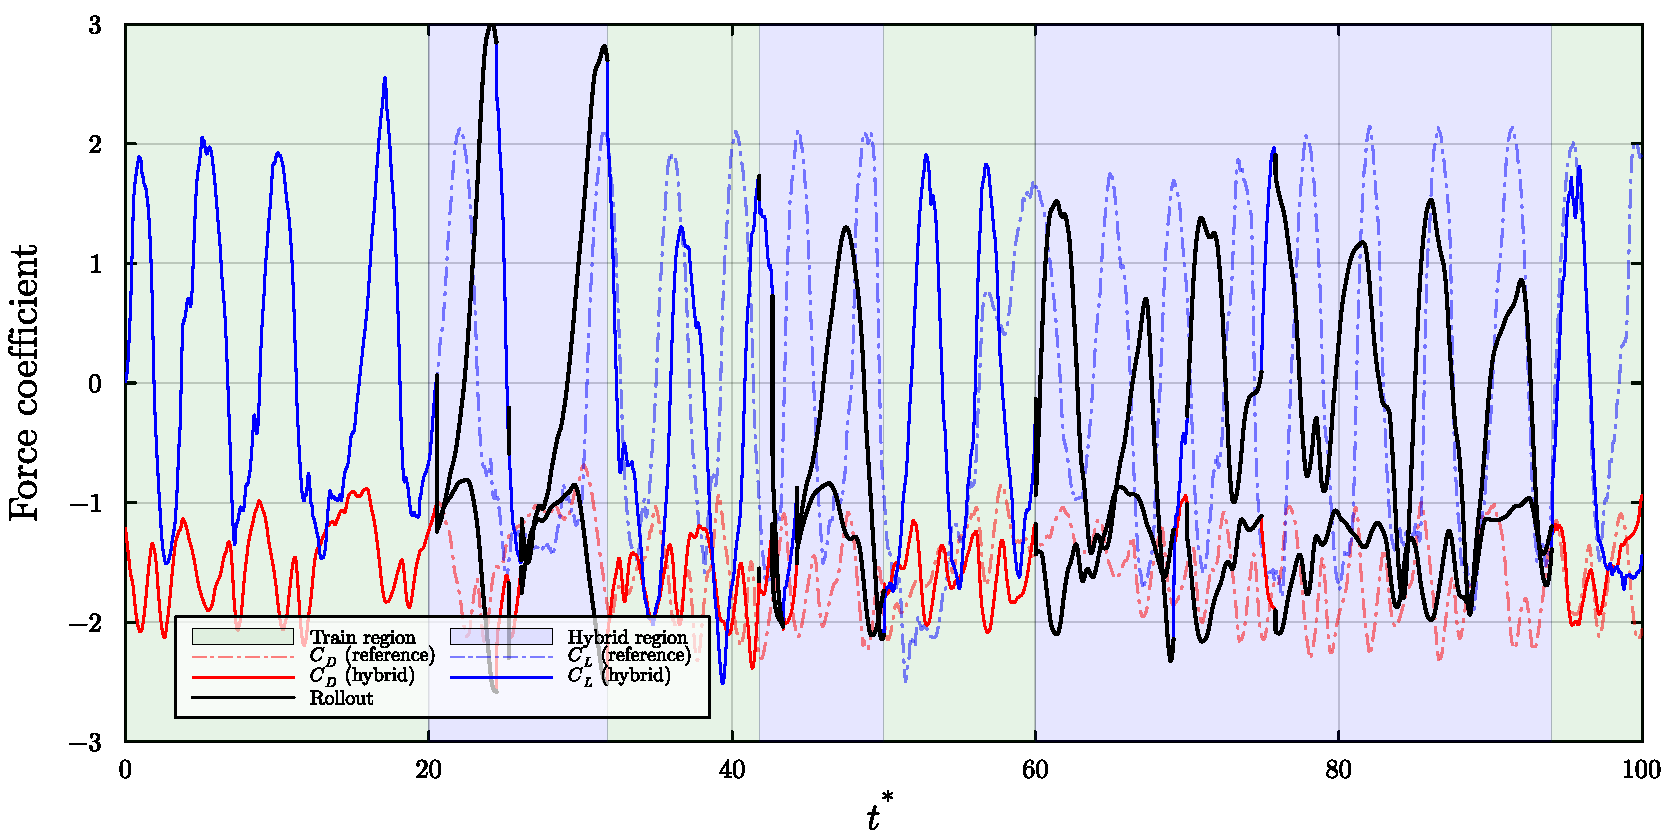
\includegraphics[width=\linewidth]{figures/Results/RE5000/hybrid_forces.pdf}
    \caption{Lift ($C_L$) and drag ($C_D$) coefficients over $t^*$ for the $Re=5000$, $512^2$ hybrid run. Reference (dash-dotted) against the hybrid loop (solid); the black trace is a single unaided rollout from $t^*=0$ with no OOD resets. Green bands mark the training region, blue bands the hybrid regions. The mean drag is held across the window, but the lift loses both amplitude and shedding signature within the hybrid regions.}    
    \label{fig: RE5000_forces}
\end{figure}


\autoref{fig: RE5000_forces} shows that the hybrid loop holds the time-mean drag but fails to reproduce the lift fluctuation: within the hybrid regions, the $C_L$ trace drifts in both amplitude and phase, and the unaided black rollout diverges from the reference entirely. This failure traces back to the near-body flow this regime produces. At $Re=5000$, the vortices form and shed through a thin, sharply varying near-wall layer, visible in the closely spaced shear structures of \autoref{fig: RE5000_vortex_shedding}, and it is precisely these complex high-gradient near-body fluctuations that the autoencoder struggles to reconstruct. The more complex the near-body fluctuations, the larger this error, so the lift, which integrates them directly, is the coefficient that suffers most.

\todo{finish on sunday say that this flow case the lift and drag fluctuations are too complex and present no clear shedding frequency for the latent dynamics to hold on to compounding with the sensitive decoder the resulting reconstructed forces are really far of from the reference. But the reference itself doesnt lend itself to being reconstructed easily due to its chaotic nature}


% \todo{at this last paragraph, tie to the fact that the pipeline has learned the general fluctuations, which is why the performance of the time averaged quantities isnt half bad, but as the performance on the lift and drag forces showed, they can't be concluded to be decent results, kind off don't say it this harshly}

% \todo{(maybe in discssion) say that this operating point shows the limits of the neural ode, but that it does also show the potential in acceleraton for the framework, be it that the dynamics it would learn would be more simple than they currently are (ie lower reynolds number)}

% \todo{have all of this written BEFORE LUNCH, after lunch, fix discussion and conclusion and then read over it to fix spelling errors}

The instantaneous reconstructions in \autoref{fig: RE5000_velocity_comp_test} show the same generalisation gap in physical space. The in-sample snapshot (\subref{fig: RE5000_velocity_comp_train}) retains the sharp shear-layer structure of the reference, whereas the held-out snapshot (\subref{fig: base_velocity_comp_right}) is visibly smoothed: the near-wake vortices lose definition and the thin separating layers blur out. This is the spatial signature of the loss gap in \autoref{fig: RE5000_loss}: the decoder reproduces the wake configurations it saw during training but regresses toward a smeared, lower-gradient field on states from the unseen window. Because the force coefficients are integrated from the decoded velocity, this near-body smoothing feeds directly into the loading, and it is the high-gradient near-wall layer, which the lift integrates most directly, that carries the amplitude and phase errors shown in \autoref{fig: RE5000_forces}.



\begin{figure}[htp]
  \centering
  \begin{subfigure}[t]{0.48\textwidth}
    \centering
    \begin{tikzpicture}
      \node[anchor=south west, inner sep=0] (img)
        {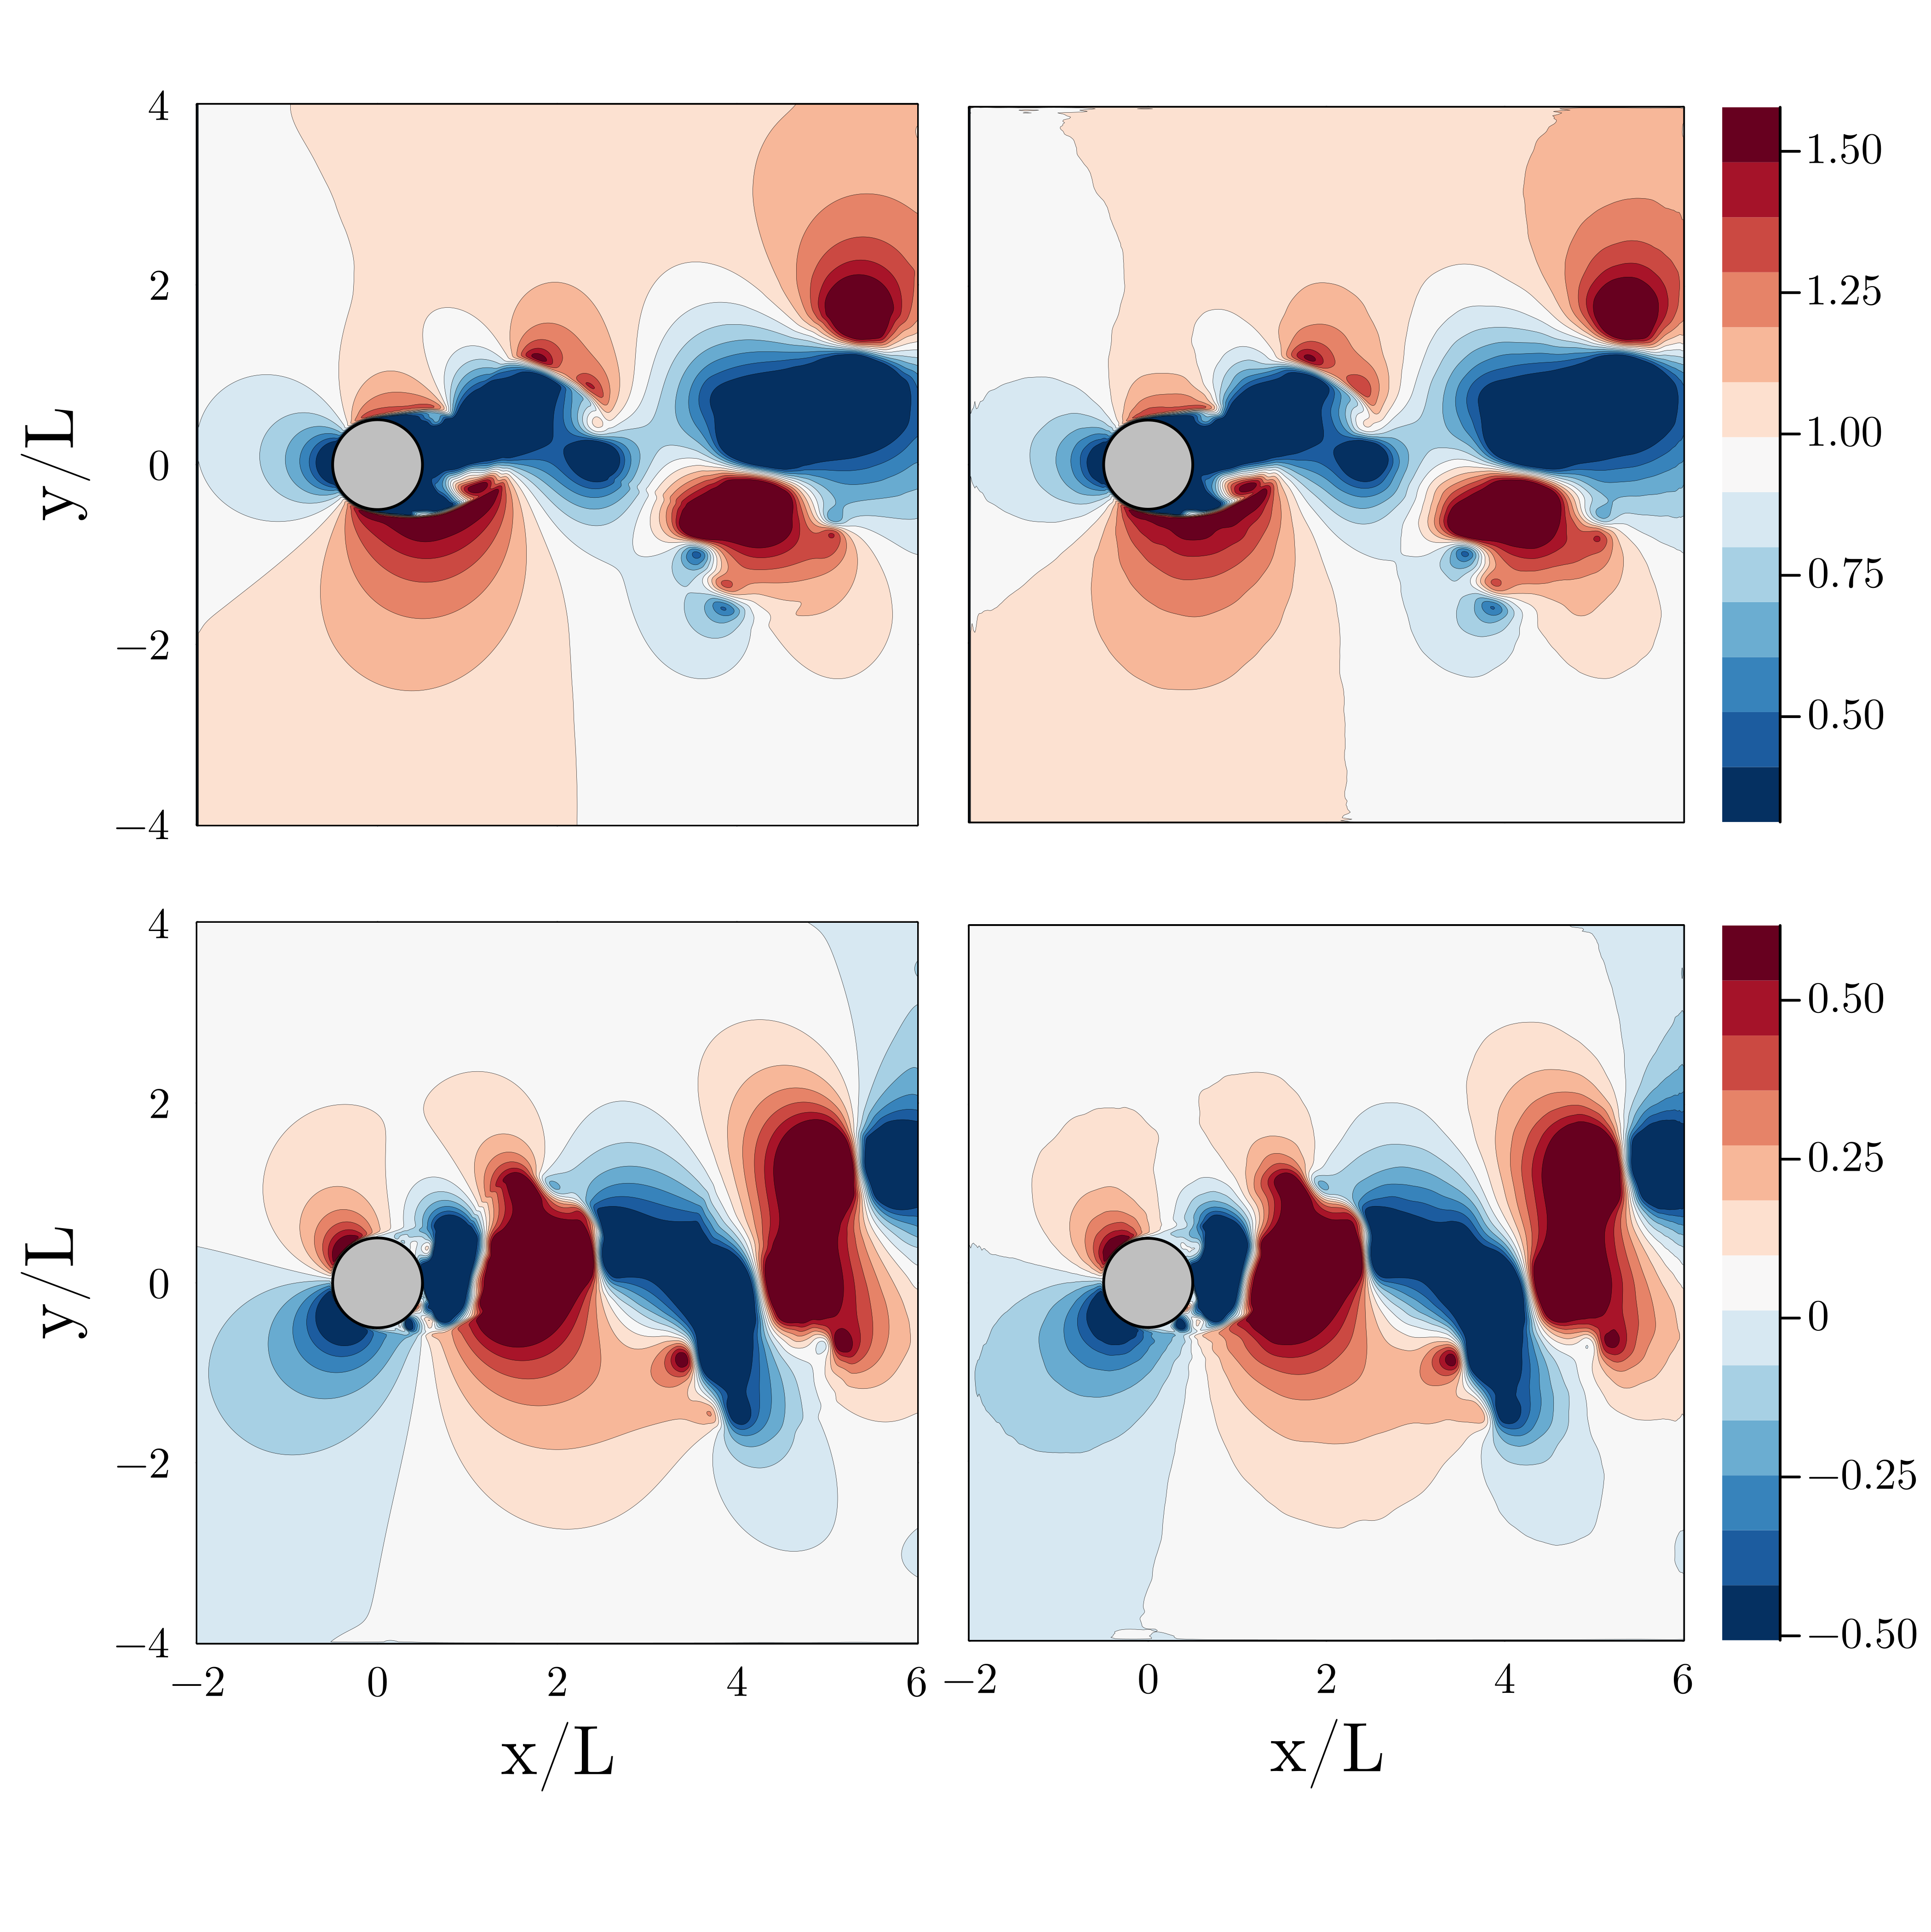
\includegraphics[width=\linewidth]{figures/Results/RE5000/velocity_comp_train.png}};
      \begin{scope}[x={(img.south east)}, y={(img.north west)}]
        % --- column headers ---
        \node[anchor=south] at (0.30, 0.95) {$\mathbf{u}$};
        \node[anchor=south] at (0.70, 0.95) {$\hat{\mathbf{u}}$};
        % --- row labels ---
      \end{scope}
    \end{tikzpicture}
    \caption{In-sample snapshot}
    \label{fig: RE5000_velocity_comp_train}
  \end{subfigure}\hfill
  \begin{subfigure}[t]{0.48\textwidth}
    \centering
    \begin{tikzpicture}
      \node[anchor=south west, inner sep=0] (img)
        {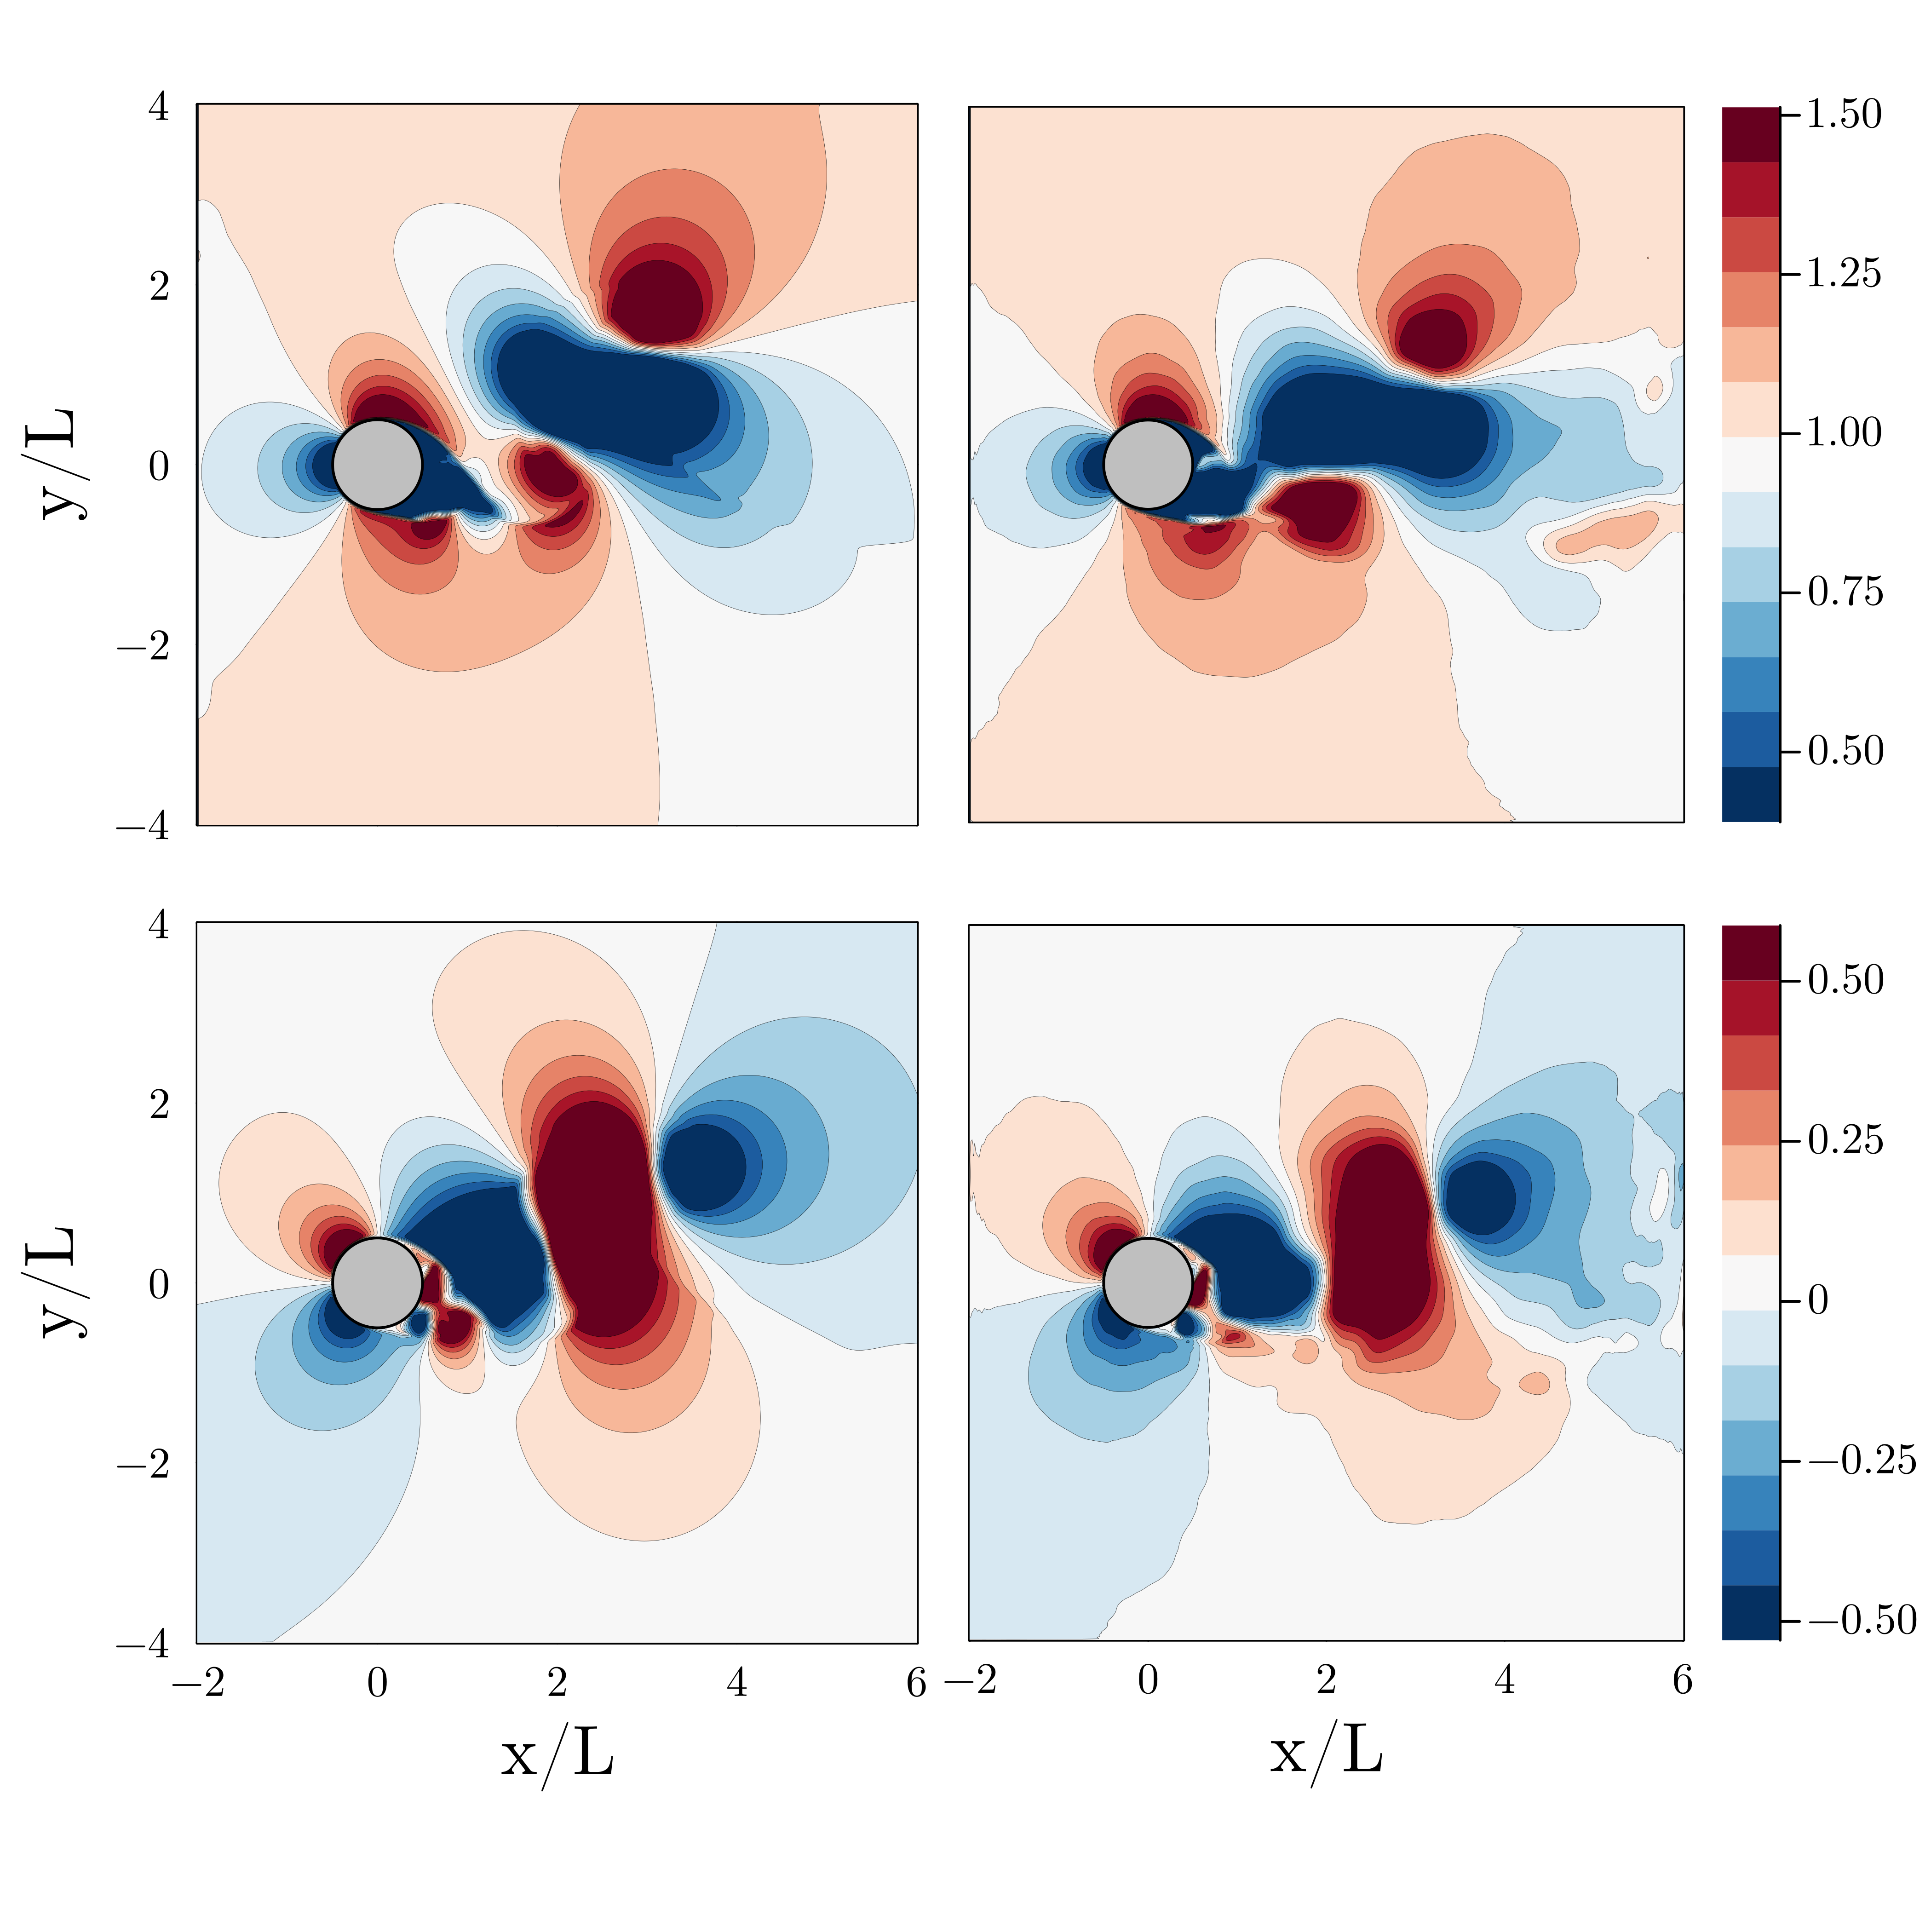
\includegraphics[width=\linewidth]{figures/Results/RE5000/velocity_comp_test.png}};
      \begin{scope}[x={(img.south east)}, y={(img.north west)}]
        \node[anchor=south] at (0.30, 0.95) {$\mathbf{u}$};
        \node[anchor=south] at (0.70, 0.95) {$\hat{\mathbf{u}}$};
      \end{scope}
    \end{tikzpicture}
    \caption{Held out snapshot}
    \label{fig: base_velocity_comp_right}
  \end{subfigure}
  \caption{Instantaneous velocity reconstruction by the autoencoder at the $Re=5000$, $512^2$ operating point for (a)~an in-sample snapshot ($t^*=6.84$) and (b)~a held-out snapshot ($t^*=19.74$). Rows: streamwise $u$ (top), transverse $v$ (bottom); within each panel, left is the WaterLily reference $\mathbf{u}$, right the reconstruction $\hat{\mathbf{u}}=\psi_\theta(\varphi_\theta(\mathbf{u}))$. The held-out field is visibly smoothed, indicating poor generalisation beyond the training distribution.}  \label{fig: RE5000_velocity_comp_test}
\end{figure}

Compared to the instantaneous reconstruction, the time-averaged statistics in \autoref{tab: re5000_field} seem to paint a better picture; the corresponding mean-velocity and Reynolds-stress contour fields, with their reference and difference maps, are shown in \autoref{app: RE5000} in \autoref{fig: RE5000_meanflow} and \autoref{fig: RE5000_rst}. The mean velocity components and all three Reynolds-stress fields correlate with the reference at $\rho>0.96$, with mean absolute errors no larger than $0.023$, and the time-mean drag is held to within $2.6\%$ over the full window. The interpretation is that $\mathcal{P}$ has learnt the statistically converged structure of the wake, even where it cannot track the instantaneous field: averaging over many shedding states recovers the low-order statistics, while the high-gradient near-body fluctuations that set the instantaneous loading are too complex to be learnt by $\mathcal{P}$. This is why the mean quantities come out well while the forces do not. The hybrid-region errors of $8.5\%$ in $\langle C_D\rangle$ and $9.2\%$ in $C_L^\text{rms}$ (\autoref{tab: re5000_forces}) are the cost of that same near-body error, and they are the honest figures here, since the smaller full-window errors are diluted by the reference segments. The integrated force metrics at this operating point, therefore, cannot be interpreted as quantitatively reliable, even though the time-averaged behaviour holds up.

\begin{table}[H]
    \centering
    \footnotesize
    \begin{subtable}[t]{0.56\textwidth}
        \centering
        \setlength{\tabcolsep}{4pt}
        \begin{tabular}{@{}lrrrr@{}}
            \toprule
            Quantity & Ref. & Hybrid & $e_\text{abs}$ & $e_\text{rel}$ [\%] \\
            \midrule
            \multicolumn{5}{l}{\textit{Full window} ($t^*\in[0,100]$)} \\
            $\langle C_D \rangle$ & $-1.56768$ & $-1.52634$ & $0.04134$ & $2.637$ \\
            $C_L^\text{rms}$      & $1.30170$  & $1.23656$  & $0.06515$ & $5.005$ \\
            \midrule
            \multicolumn{5}{l}{\textit{Hybrid regions only}} \\
            $\langle C_D \rangle$ & $-1.57821$ & $-1.44368$ & $0.13452$ & $8.524$ \\
            $C_L^\text{rms}$      & $1.29928$  & $1.17933$  & $0.11995$ & $9.232$ \\
            \bottomrule
        \end{tabular}
        \caption{Integrated force coefficients: time-mean drag
        $\langle C_D \rangle$ and r.m.s.\ lift $C_L^\text{rms}$ against the
        reference, with absolute and relative errors.}
        \label{tab: re5000_forces}
    \end{subtable}
    \hfill
    \begin{subtable}[t]{0.40\textwidth}
        \centering
        \setlength{\tabcolsep}{5pt}
        \begin{tabular}{@{}lrr@{}}
            \toprule
            Quantity & $\varepsilon$ (MAE) & $\rho$ \\
            \midrule
            \multicolumn{3}{l}{\textit{Mean flow}} \\
            $\langle u \rangle$    & $0.023$ & $0.9773$ \\
            $\langle v \rangle$    & $0.012$ & $0.9761$ \\
            \midrule
            \multicolumn{3}{l}{\textit{Reynolds stresses}} \\
            $\langle u'u' \rangle$ & $0.010$ & $0.9825$ \\
            $\langle v'v' \rangle$ & $0.015$ & $0.9932$ \\
            $\langle u'v' \rangle$ & $0.006$ & $0.9626$ \\
            \bottomrule
        \end{tabular}
        \caption{Time-averaged field statistics over $\Omega$: mean absolute
        error $\varepsilon$ and spatial correlation $\rho$.}
        \label{tab: re5000_field}
    \end{subtable}
    \caption{Hybrid-loop accuracy at $Re=5000$.
    (a) integrated loading; (b) mean-flow and Reynolds-stress fields.}
    \label{tab: re5000_accuracy}
\end{table}

All in all, the performance of $\mathcal{P}$ shows a split outcome at this operating point: the autoencoder reconstructs the wake states it has seen but smooths those drawn from the held-out window, so the instantaneous loading is unreliable when trying to predict outside of the training window; while the time-averaged velocity and Reynolds-stress fields remain faithful to the reference. The source of error at this operating point can not be blamed on the autoencoder alone, since the loading is only as good as the decoded velocity field, and that field is in turn only as good as the latent trajectory the Neural ODE supplies, so the reconstruction ceiling set here does not yet distinguish error baked in by the autoencoder from drift accumulated during the latent integration. 


\subsubsection{Latent Dynamics}

The latent dynamics inherit the underlying wake's chaos. \autoref{fig: RE5000_trajectories} shows that the reference latent components carry no clean periodicity: unlike \autoref{fig: Re250_latent_traj}, where each component traces a near-sinusoidal orbit at the shedding frequency, the $Re=5000$ trajectories are irregular in both amplitude and phase, with no simple frequency to which the components return. The chaos that hampered the instantaneous velocity reconstruction is therefore already present in the latent state $\mathbf{z}=\varphi_\theta(\mathbf{u})$ itself.

\begin{figure}[htbp]
    \centering
    \begin{subfigure}[t]{0.48\textwidth}
        \centering
        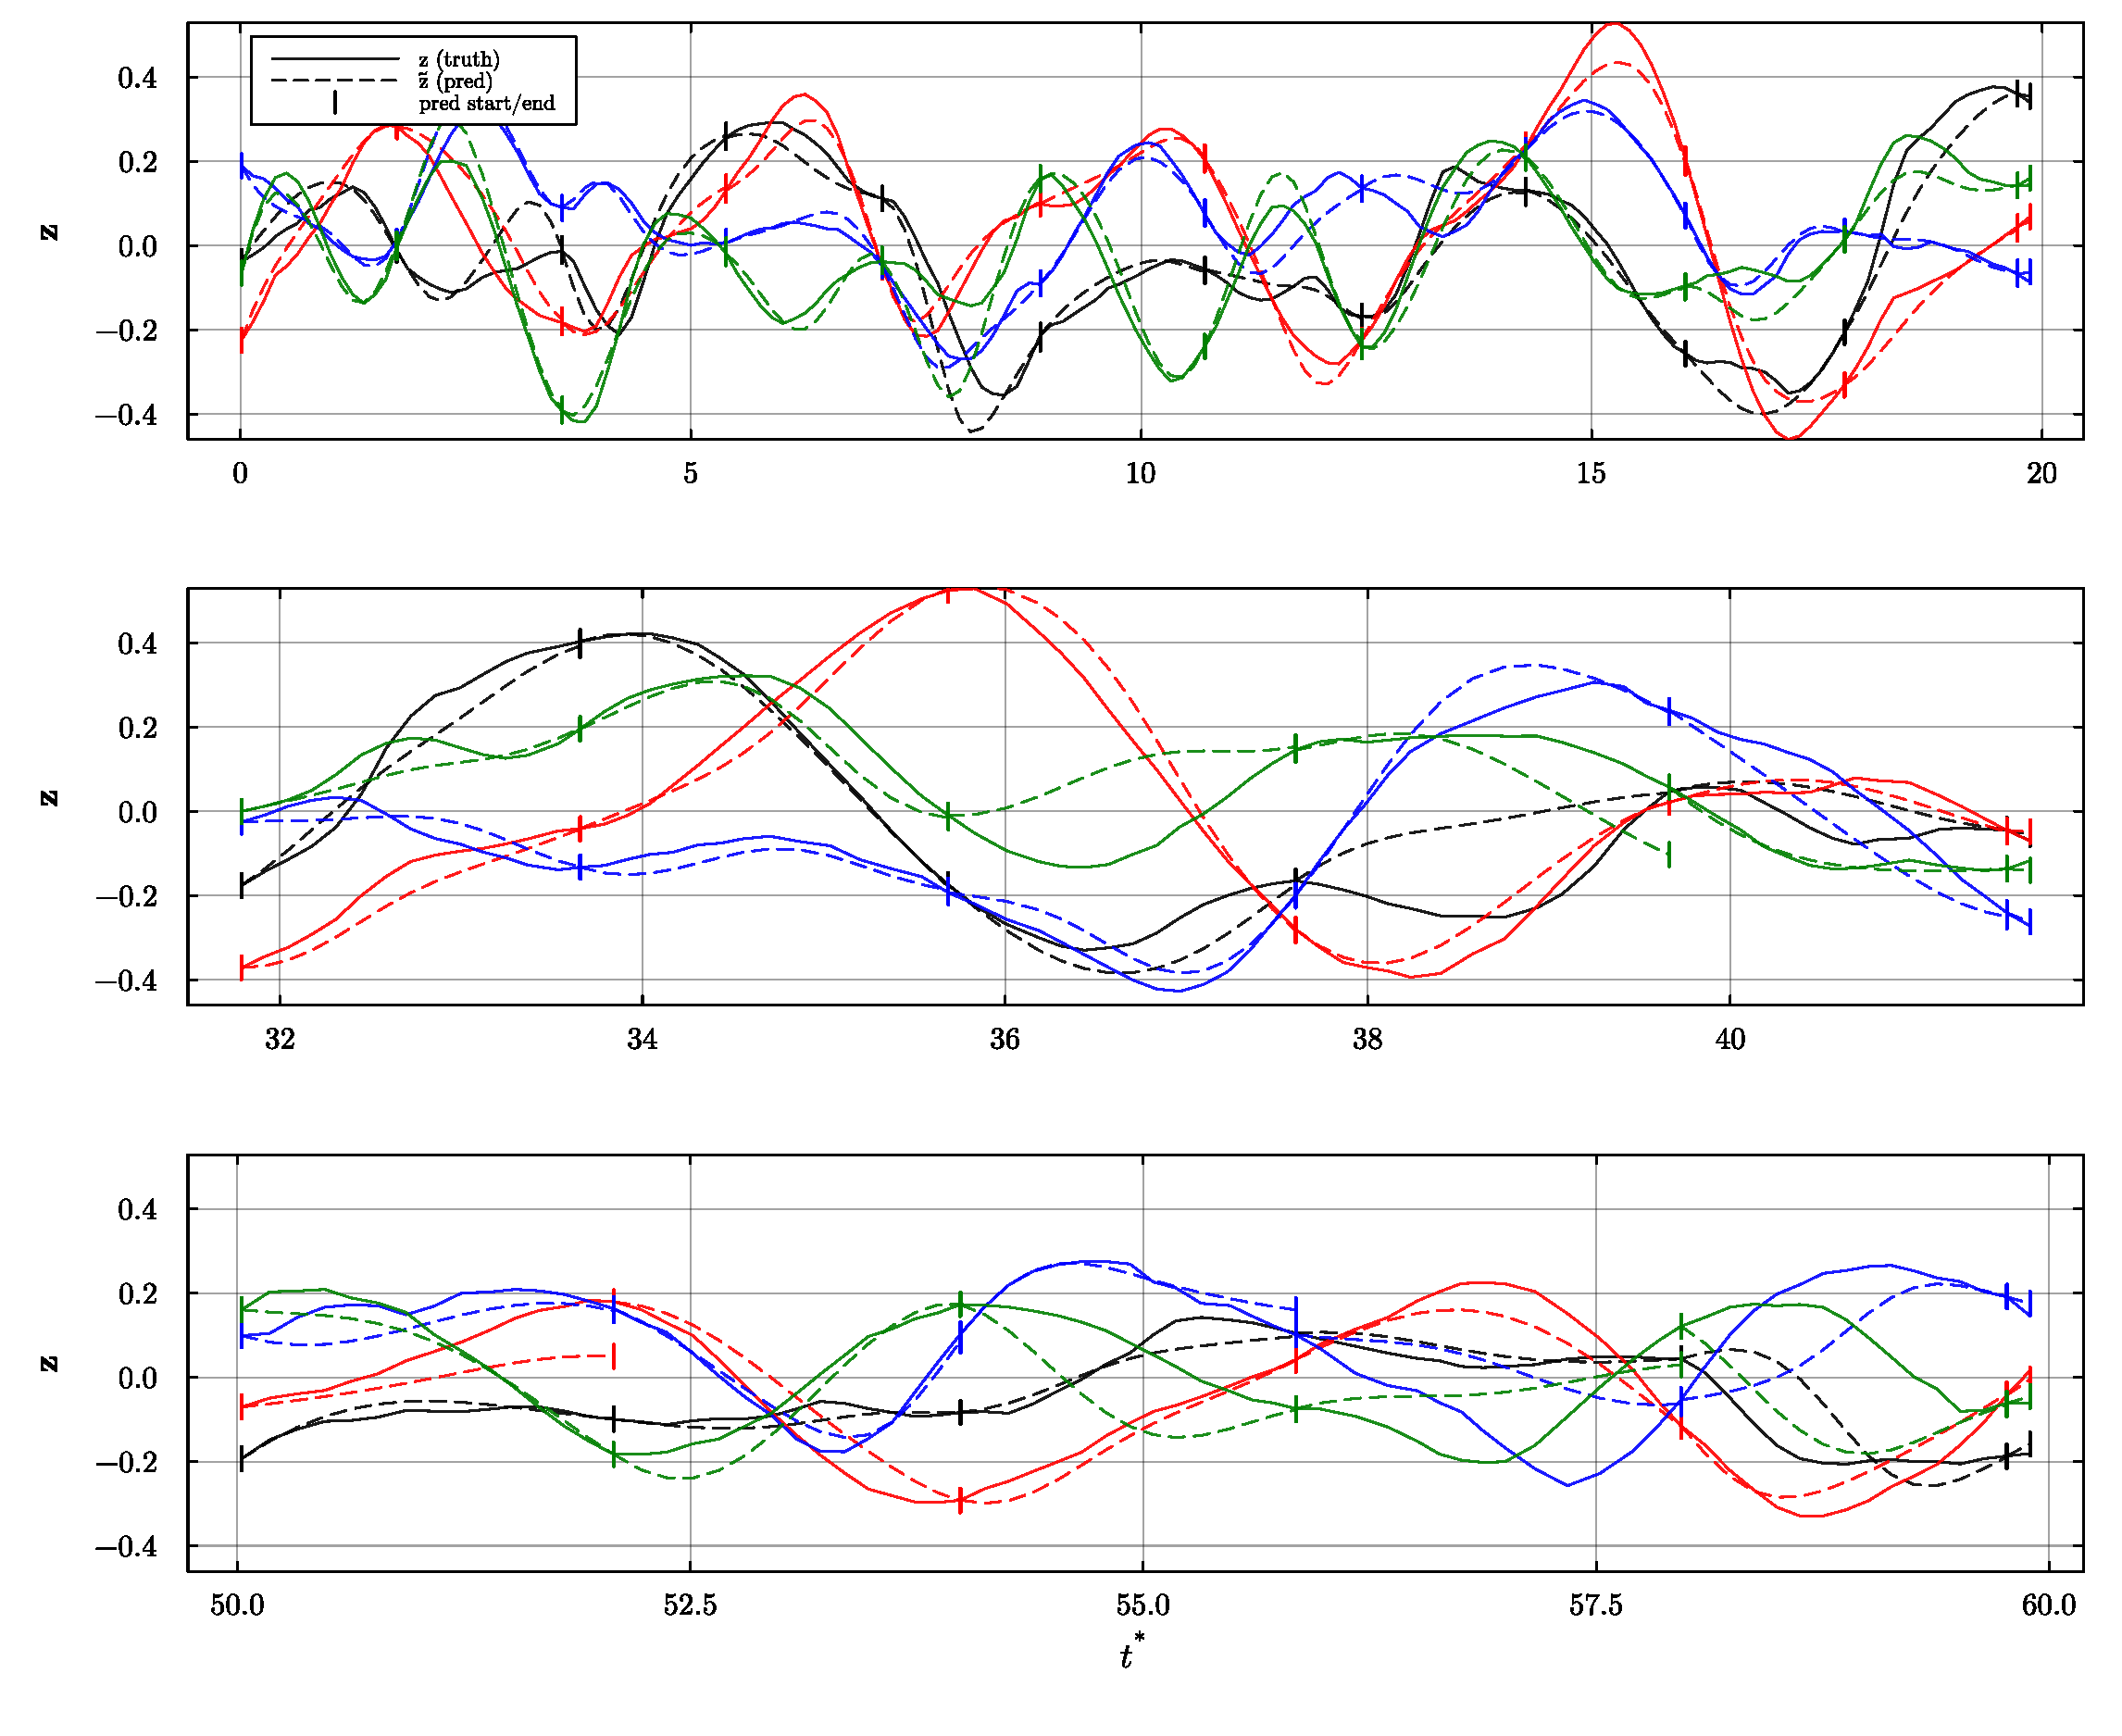
\includegraphics[width=\linewidth]{figures/Results/RE5000/trajectories.pdf}
    \caption{Converged multiple-shooting fit on the augmented trajectory set; markers denote shooting-segment boundaries.}
    \label{fig: RE5000_retrain_node_ms}
    \end{subfigure}
    \begin{subfigure}[t]{0.48\textwidth}
        \centering
        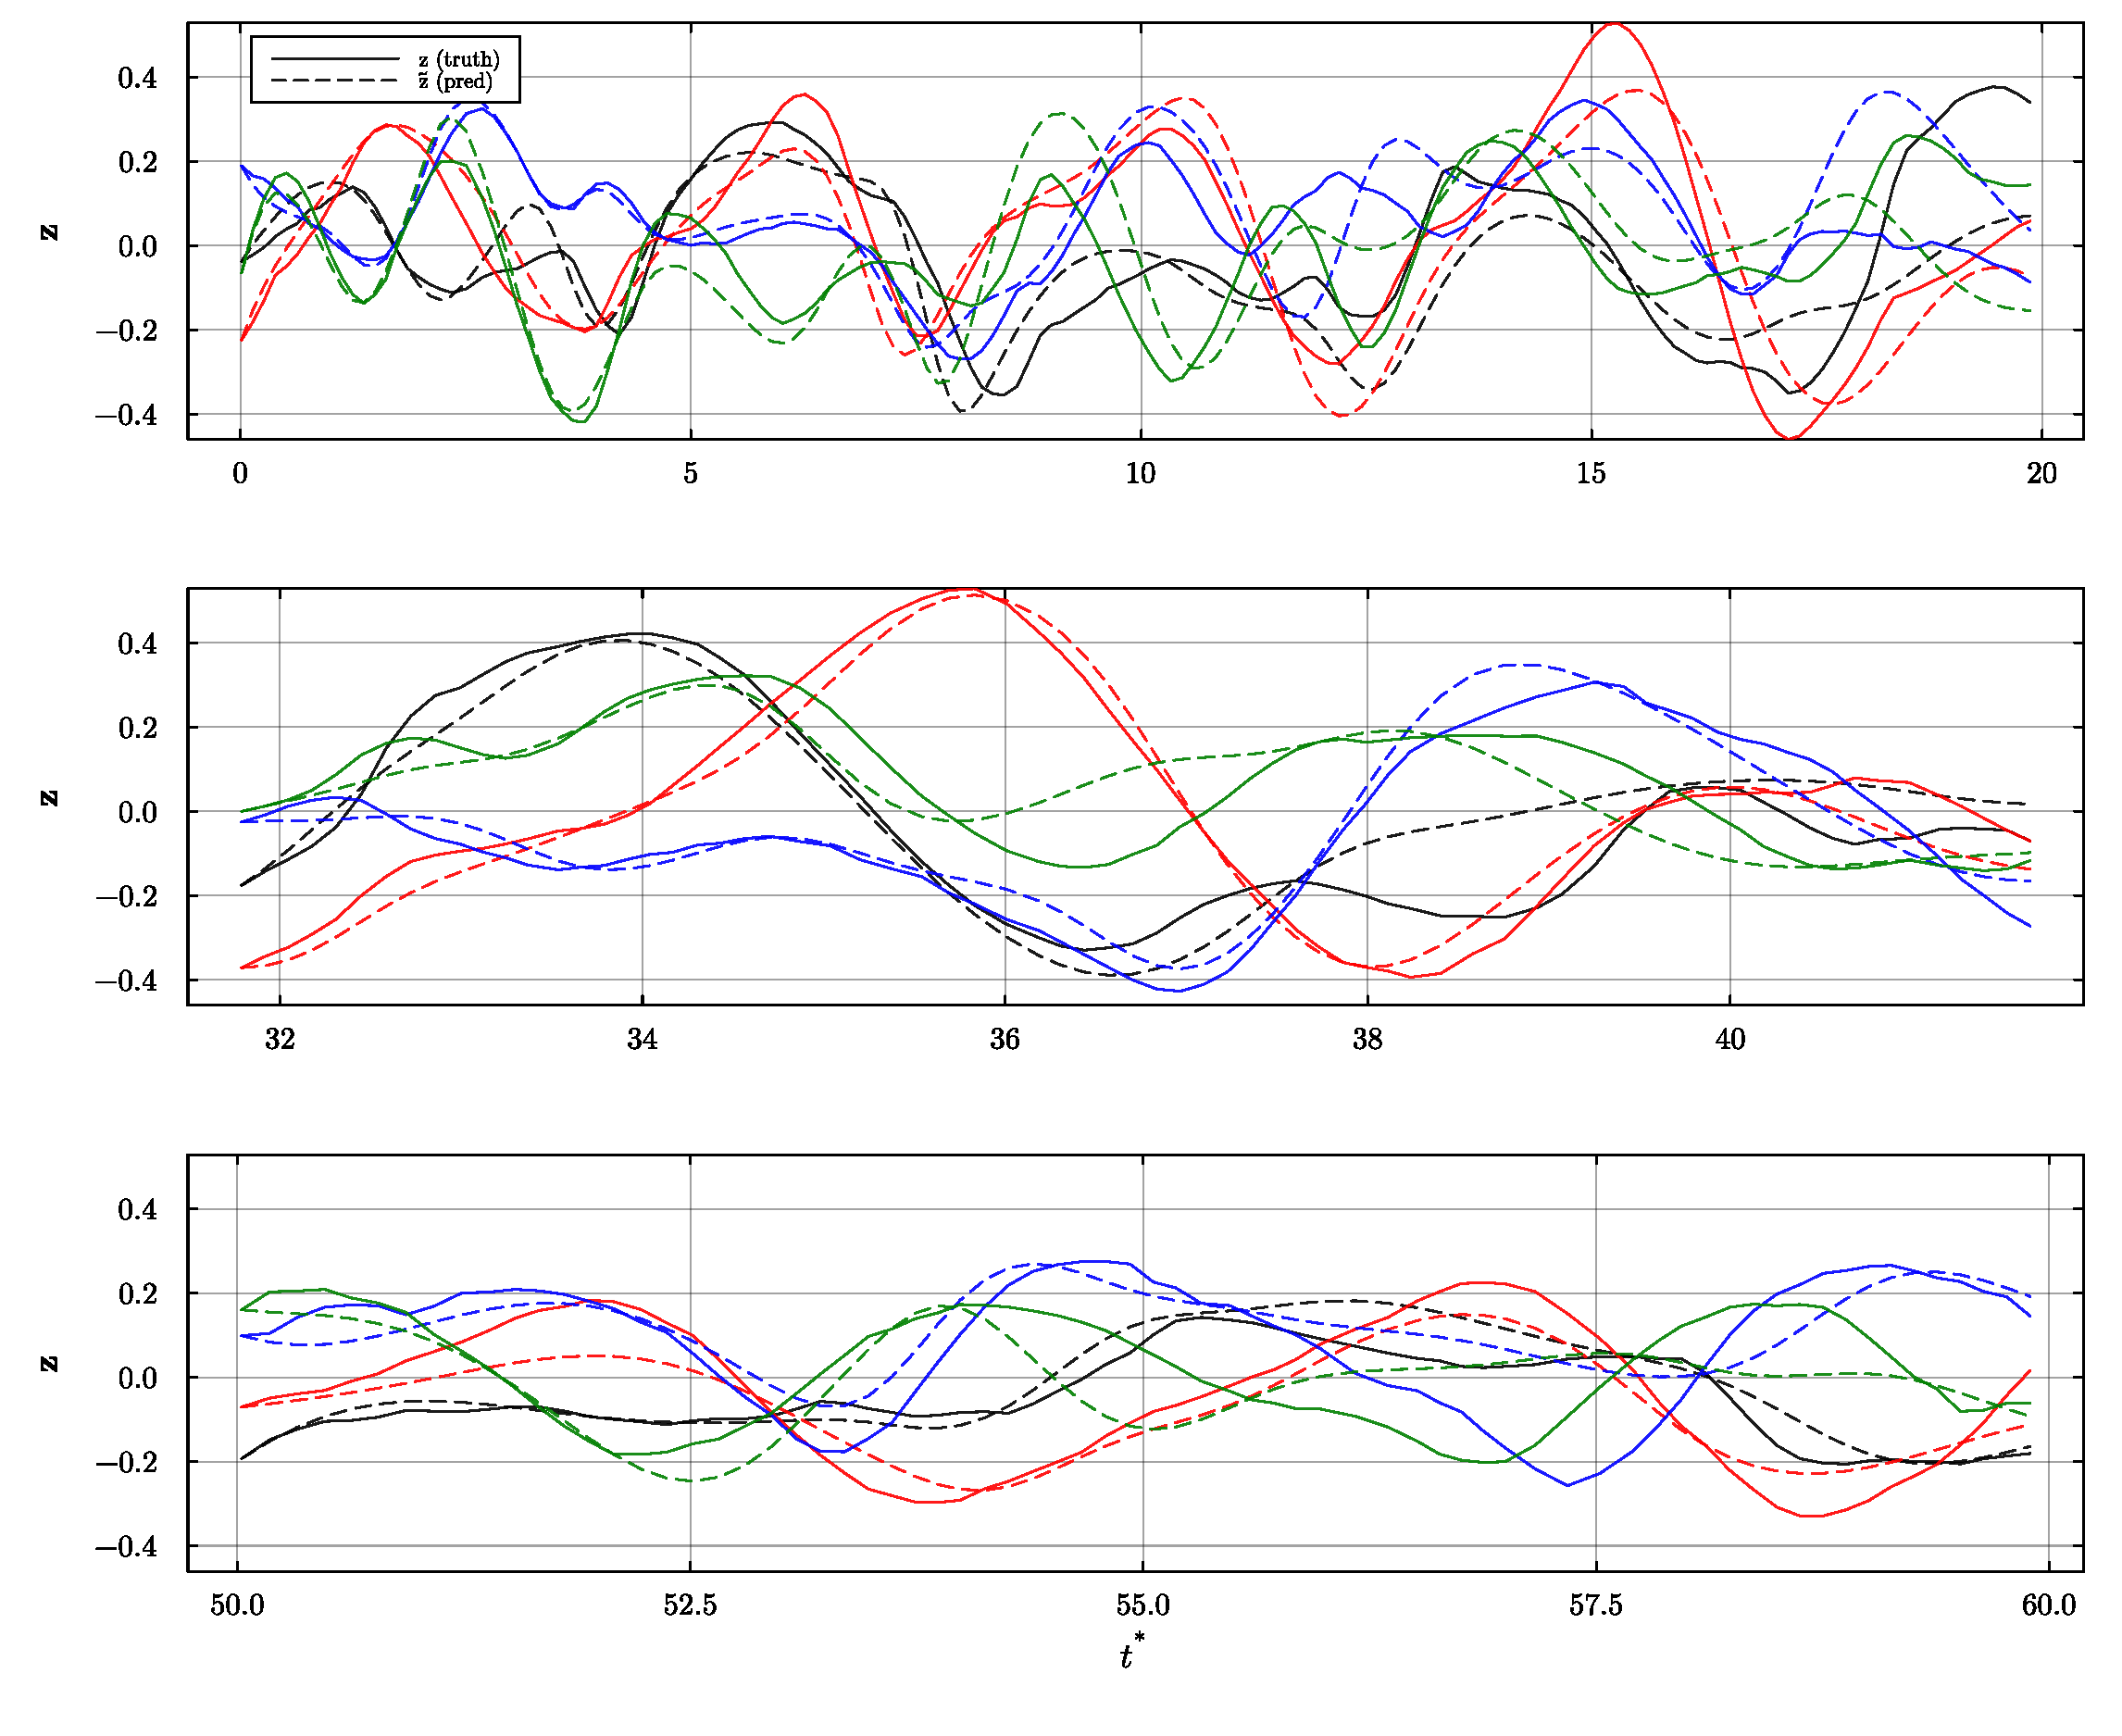
\includegraphics[width=\linewidth]{figures/Results/RE5000/rollout_single_shooting.pdf}
    \caption{Single rollout from $t^*=0$ across both windows after the second retraining, no segment resets.}
    \label{fig: RE5000_retrain_node_singleshoot}
    \end{subfigure}
    \caption{Latent dynamics of $f_\phi$  of the $Re=5000$, $512^2$ operating point, four representative components shown over all time windows. Reference $z$ (solid) against prediction $\tilde{z}$ (dashed). (a) Converged multiple-shooting fit on the augmented trajectory set, with segment start/end markers; (b) unaided single rollout from $t^*=0$ over the same windows.}
    \label{fig: RE5000_trajectories}
\end{figure}

Against this reference, $f_\phi$ recovers the latent dynamics reasonably well under multiple shooting but not during free rollout. In \autoref{fig: RE5000_retrain_node_ms}, the converged multiple-shooting fit tracks the reference closely within each shooting segment, but this good visual performance is mainly due to the multiple-shooting training: each segment is re-anchored to the reference latent state at its start (the segment markers). The single rollout from $t^*=0$ in \autoref{fig: RE5000_retrain_node_singleshoot} is the unflattering test, and there the prediction $\hat{\mathbf{z}}$ drifts away from the reference within a few windows. The single-shot rollouts track the learned frequencies to some extent but diverge at the end of each trajectory window. These unguarded rollouts show that $f_\phi$ has learnt the dynamics of the latent state, but due to the chaotic nature of the rollout, rollout drift can set in quickly. This is similar to the way the force rollout of \autoref{fig: RE5000_forces} also drifts to unknown states. The latent divergence and the force divergence are therefore connected behaviours.

The chaotic nature of the latent dynamics is what loosens the KNN monitor. Because the latent trajectories never settle onto a tight orbit, the training set populates a broad, high-variance region of latent space, and the KNN gating threshold $\tau$ derived from it is correspondingly large; it also climbs across the retraining stages (\autoref{tab: re5000_rollout_summary}), from $\tau=0.614$ for the initial model to $0.898$ and $0.902$ after the first and second retrains, as each augmented training set widens the accepted region further.  A large $\tau$ is a lenient gate: a rollout must drift far before its score crosses the threshold and triggers a reset. 

\begin{table}[htbp]
  \centering
  \footnotesize
  \setlength{\tabcolsep}{4pt}
  \renewcommand{\arraystretch}{0.85}
  \begin{tabular}{clrrrcc}
    \toprule
    \# & NODE model & Steps & $\Delta t^*$ & $t^*_\text{r, end}$ & score & $\tau$ \\
    \midrule
    1 & initial      & 717  & 4.470  & 24.470 & 0.615 & 0.614 \\
    2 & initial      & 1    & 0.811  & 25.281 & 0.855 & 0.614 \\
    3 & initial      & 1035 & 6.502  & 31.783 & 0.615 & 0.614 \\
    \midrule
    4 & 1st retrain  & 2    & 10.021 & 41.804 & 0.899 & 0.898 \\
    5 & 1st retrain  & 126  & 1.556  & 43.360 & 0.899 & 0.898 \\
    6 & 1st retrain  & 1049 & 6.656  & 50.017 & 0.898 & 0.898 \\
    \midrule
    7 & 2nd retrain  & 1661 & 19.094 & 69.110 & 0.903 & 0.902 \\
    8 & 2nd retrain  & 895  & 5.802  & 74.912 & 0.903 & 0.902 \\
    9 & 2nd retrain  & 3329 & 19.130 & 94.042 & 0.904 & 0.902 \\
    \bottomrule
  \end{tabular}
  \caption{Per-rollout summary of the KNN-gated NODE inference at $Re = 5000$. Every accepted rollout terminates just above the active threshold $\tau$.}
  \label{tab: re5000_rollout_summary}
\end{table}

The consequence is visible in the \texttt{Steps} and $\Delta t^*$ columns, where accepted rollouts are allowed to run for hundreds to thousands of integration steps, the longest covering $\Delta t^* \approx 19$ time units in a single uninterrupted rollout. This long rollout at the end of the simulation window is, however, not entirely erroneous, as \autoref{fig: RE5000_forces} shows; it still traces the reference, but it is significantly more diffuse than the reference, showing how the rollout matches one of the characteristic frequencies of the shedding regime, indicating that $f_\phi$ has managed to learn this specific flow behaviour. Which is exactly what \autoref{fig: RE5000_forces} also indicated with the matching, but diverging, unguarded rollouts

The latent dynamics at the $Re=5000$, $512^2$ operating point expose a contradiction in the KNN gating strategy. The chaotic latent space sets $\tau$ from the spread of the training distribution, so the threshold scales with how disordered that distribution is. This means that a well-performing autoencoder that produces a clean, near-periodic wake yields a tight latent cluster, a small $\tau$, and a strict gate that resets often, thereby capping rollout length and limiting the achievable speedup, as in \autoref{subsect: 4_re250}. The chaotic $Re=5000$ wake does the opposite: its complex latent distribution inflates $\tau$, the gate turns lenient, and rollouts are allowed to run for thousands of steps, exactly the regime in which $f_\phi$ accumulates the most drift.  The monitor is therefore most permissive where the dynamics are hardest to predict and most restrictive where they are easiest to predict, which is the wrong way round. This is not a tuning error but a consequence of deriving the threshold from in-distribution variance: the harder the flow is to learn, the more freedom the gate hands the part of the pipeline least able to use it.


%-------------------------------------------------------------------------------------------------------------

% \subsection{Finer Simulation grid}
\label{subsect: 4_finer}
As established in \autoref{subsect: 4_wall_time}, the per-CTU advantage of the latent rollout is tied to the base-case resolution: since the WaterLily solver is memory-bound, its cost per CTU grows with the grid size~\cite{Weymouth2025}, whereas a single rollout of $\mathcal{P}$ is fixed by the latent dimension $N_z = 16$ and is independent of the grid. The $256^2$ baseline used throughout this work is therefore a comparatively cheap case in which to demonstrate the gain. To investigate the effects of the hybrid loop on more expensive simulations, the reference case is re-run on a refined $512^2$ grid, keeping the Reynolds number, domain, and cylinder geometry of \autoref{tab: parameters} fixed, so that only the spatial discretisation changes. The following paragraphs will quantify how grid refinement affects the cost per CTU of the reference solver and the resulting upper bound on the achievable acceleration, together with the resolved wake itself, since a finer grid captures the secondary vortex structures of the $Re=2500$ flow more sharply, as displayed in \autoref{fig: finer_vortex_shedding}, and shifts the integrated force statistics on which the hybrid loop is assessed.


\begin{figure}[htbp]
    \centering
    \begin{subfigure}[b]{0.19\textwidth}
        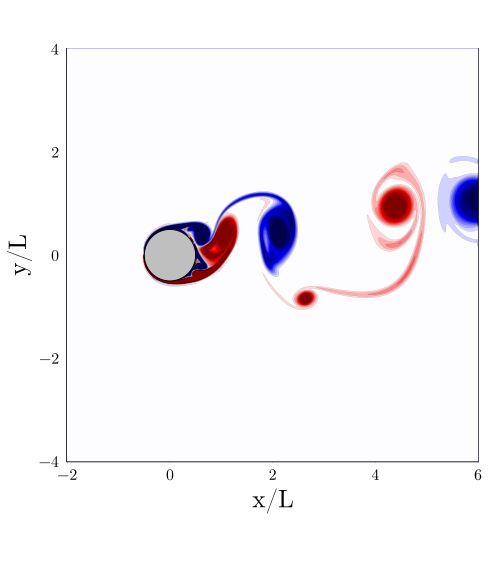
\includegraphics[width=\textwidth]{figures/Results/finer/contours/shedding_t0.1.png}
        \caption{$t^*_{n}$}
    \end{subfigure}
    \begin{subfigure}[b]{0.19\textwidth}
        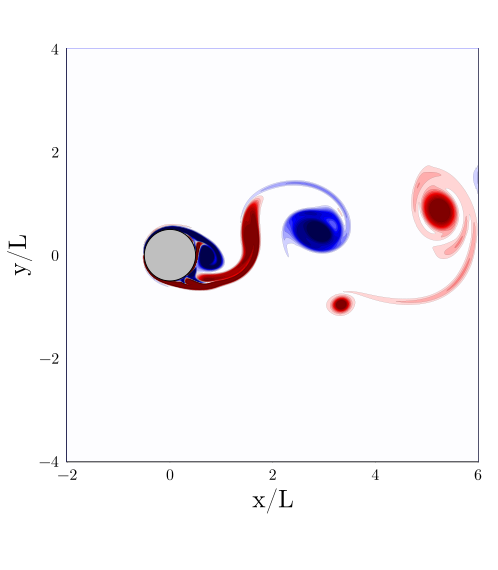
\includegraphics[width=\textwidth]{figures/Results/finer/contours/shedding_t1.1.png}
        \caption{$t^*_{n+\Delta t}$}
    \end{subfigure}
    \begin{subfigure}[b]{0.19\textwidth}
        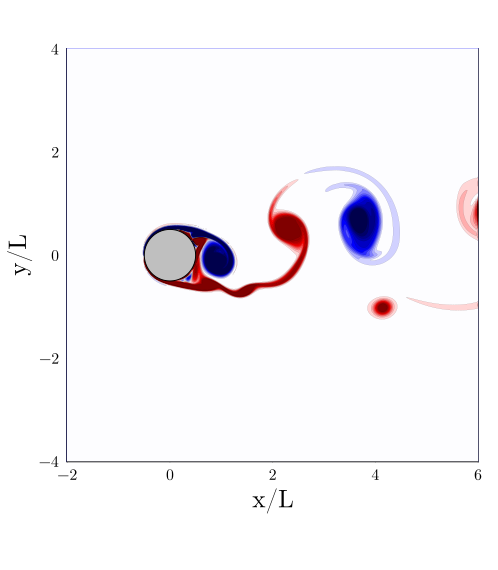
\includegraphics[width=\textwidth]{figures/Results/finer/contours/shedding_t2.1.png}
        \caption{$t^*_{n+ 2\Delta t}$}
    \end{subfigure}
    \begin{subfigure}[b]{0.19\textwidth}
        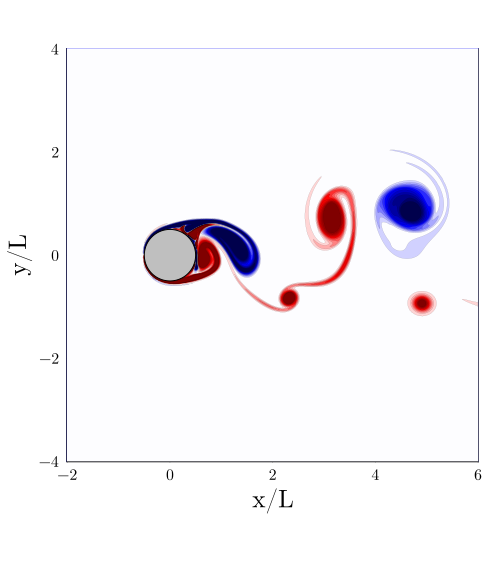
\includegraphics[width=\textwidth]{figures/Results/finer/contours/shedding_t3.1.png}
        \caption{$t^*_{n+ 3\Delta t}$}
    \end{subfigure}
    \begin{subfigure}[b]{0.19\textwidth}
        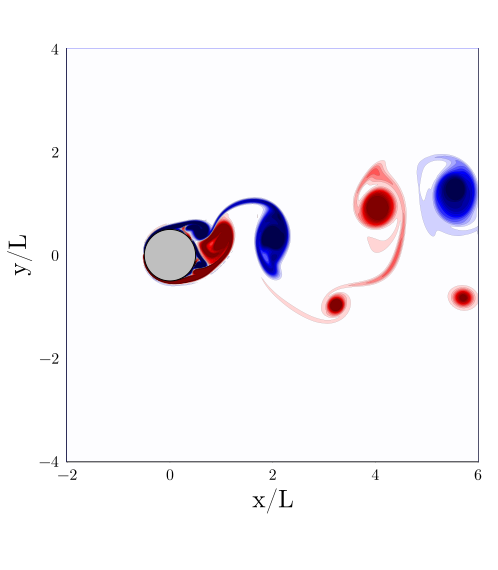
\includegraphics[width=\textwidth]{figures/Results/finer/contours/shedding_t4.2.png}
        \caption{$t^*_{n+ 4\Delta t}$}
    \end{subfigure}
    \caption{Instantaneous vorticity field $\nicefrac{\omega L}{U}$ of the finer ($512^2$) reference simulation at $Re=2500$, shown for five consecutive snapshots (left to right). Positive (red) and negative (blue) vorticity, the refined grid resolves the secondary (small-scale) structures in the wake more sharply than the $256^2$ baseline.}
    \label{fig: finer_vortex_shedding}
\end{figure}

\subsection{Wall-Time Performance}
\label{subsect: 4_finer_walltime}

Following the wall clock breakdown in \autoref{subsect: 4_wall_time}, the refined hybrid simulation is broken down into its segments, and their wall times are presented in \autoref{tab: wall_timing_hybrid_finer}. Just as in the base simulation, the initial autoencoder training consumes a very high fraction of $\mathcal{S} $'s total wall time, about $45\%$ of the total, and once the two retraining cycles are added, building and updating the networks accounts for close to $90\%$ of the $3768$~s pipeline. The CFD work, the initial data-gathering, and the two snapshot-gathering runs make up most of what remains, while the latent rollouts contribute less than $1\%$.

\begin{table}[htp]
    \centering
    \begin{tabular}{llrr}
        \toprule
        Phase & Component & Time (s) & \% of total \\
        \midrule
        initial data-gathering & -- & 190.80 & 5.06 \\
        \midrule
        \multirow{2}{*}{Train} & AE   & 1704.00 & 45.22 \\
                               & NODE &  222.00 &  5.89 \\
        \midrule
        \multirow{3}{*}{Hybrid section 1} & CFD + rollout & 1.673 & 0.04 \\
                                          & CFD + rollout & 4.057 & 0.11 \\
                                          & CFD + rollout & 4.183 & 0.11 \\
        \midrule
        \multirow{3}{*}{Retrain 1} & Gather snapshots &  95.40 &  2.53 \\
                                   & AE               & 462.00 & 12.26 \\
                                   & NODE             & 168.00 &  4.46 \\
        \midrule
        \multirow{3}{*}{Hybrid section 2} & CFD + rollout & 0.013 & 0.00 \\
                                          & CFD + rollout & 3.008 & 0.08 \\
                                          & CFD + rollout & 4.117 & 0.11 \\
        \midrule
        \multirow{3}{*}{Retrain 2} & Gather snapshots &  95.40 &  2.53 \\
                                   & AE               & 606.00 & 16.08 \\
                                   & NODE             & 204.00 &  5.41 \\
        \midrule
        Hybrid section 3 & CFD + rollout & 3.232 & 0.09 \\
        \midrule
        \textbf{Total} & & \textbf{3767.88} & \textbf{100.00} \\
        \bottomrule
    \end{tabular}
    \caption{Wall-clock breakdown of the hybrid simulation pipeline (finer $512^2$ run).}
    \label{tab: wall_timing_hybrid_finer}
\end{table}

As mentioned, the rollout cost barely changes with the grid. It is fixed by the latent dimension $N_z = 16$ and stays around $85$~ms/CTU, the same order as the base run, because it never touches the full field. The WaterLily time integrations, on the other hand, now cost $9540$~ms/CTU, against $866$~ms/CTU at $256^2$. This large cost difference between rollout and CFD is even more noticeable when inspecting the acceleration metrics, $S_\text{loop}$: 

\begin{align}
    S_\text{loop}
    &= \frac{T_\text{wall}^\text{ref}}{T_\text{wall}^\text{h, tot}}
    = \frac{954.84}{401.883} = 2.38
\end{align}

Showing that the hybrid loop uses the low-cost rollouts to its full effect, where it is able to achieve a $2.38$ speedup compared to the reference simulation. To assess the speedup of the hybrid loop compared to the training cost of the ML components of $\mathcal{P}$, the training wall time is added to the comparison in $S_\text{eff}$ with $T_\text{wall}^\text{h, training} = 3566$~s of training.

\begin{align}
    S_\text{eff}
    &= \frac{T_\text{wall}^\text{ref}}{T_\text{wall}^\text{h, tot} + T_\text{wall}^\text{h, training}}
    = \frac{954.84}{401.883 + 3366}
    = \frac{954.84}{3767.88} \approx 0.25
\end{align}

A single finer run is therefore still much slower than simply running $\mathcal{S}_\text{ref}$, because the training cost is not repaid within one simulation window. But it still performs better than the base case, which achieved an effective speedup of $0.073$, indicating that refining the grid begins to close part of the gap between the full pipeline and running the reference simulation. 

\subsection{Spatial and physical fidelity}
The finer simulation is passed to $\mathcal{P}$ without any architectural change: the architectures of $\varphi_\theta$, $\psi_\theta$ and $f_\phi$ of \autoref{sect: 4_base_hybrid} are reused as-is. The only change to the architecture is the input and output dimensions of the autoencoder, so that they can correctly pass the new, finer grid down to the latent space without dimension mismatches. An advantage of the refinement is that the decoder's
fixed cell-width smoothing now spans half the physical width, compared to the base architecture. This means that the thin separating shear layers that dominated the base-grid reconstruction error (\autoref{fig: base_velocity_comp}) are resolved by roughly twice as many cells and blurred less in physical space. Because the autoencoder can now capture fine dynamics to a much higher degree, the cost function converges much faster than before. 


\begin{figure}[htp]
    \centering
    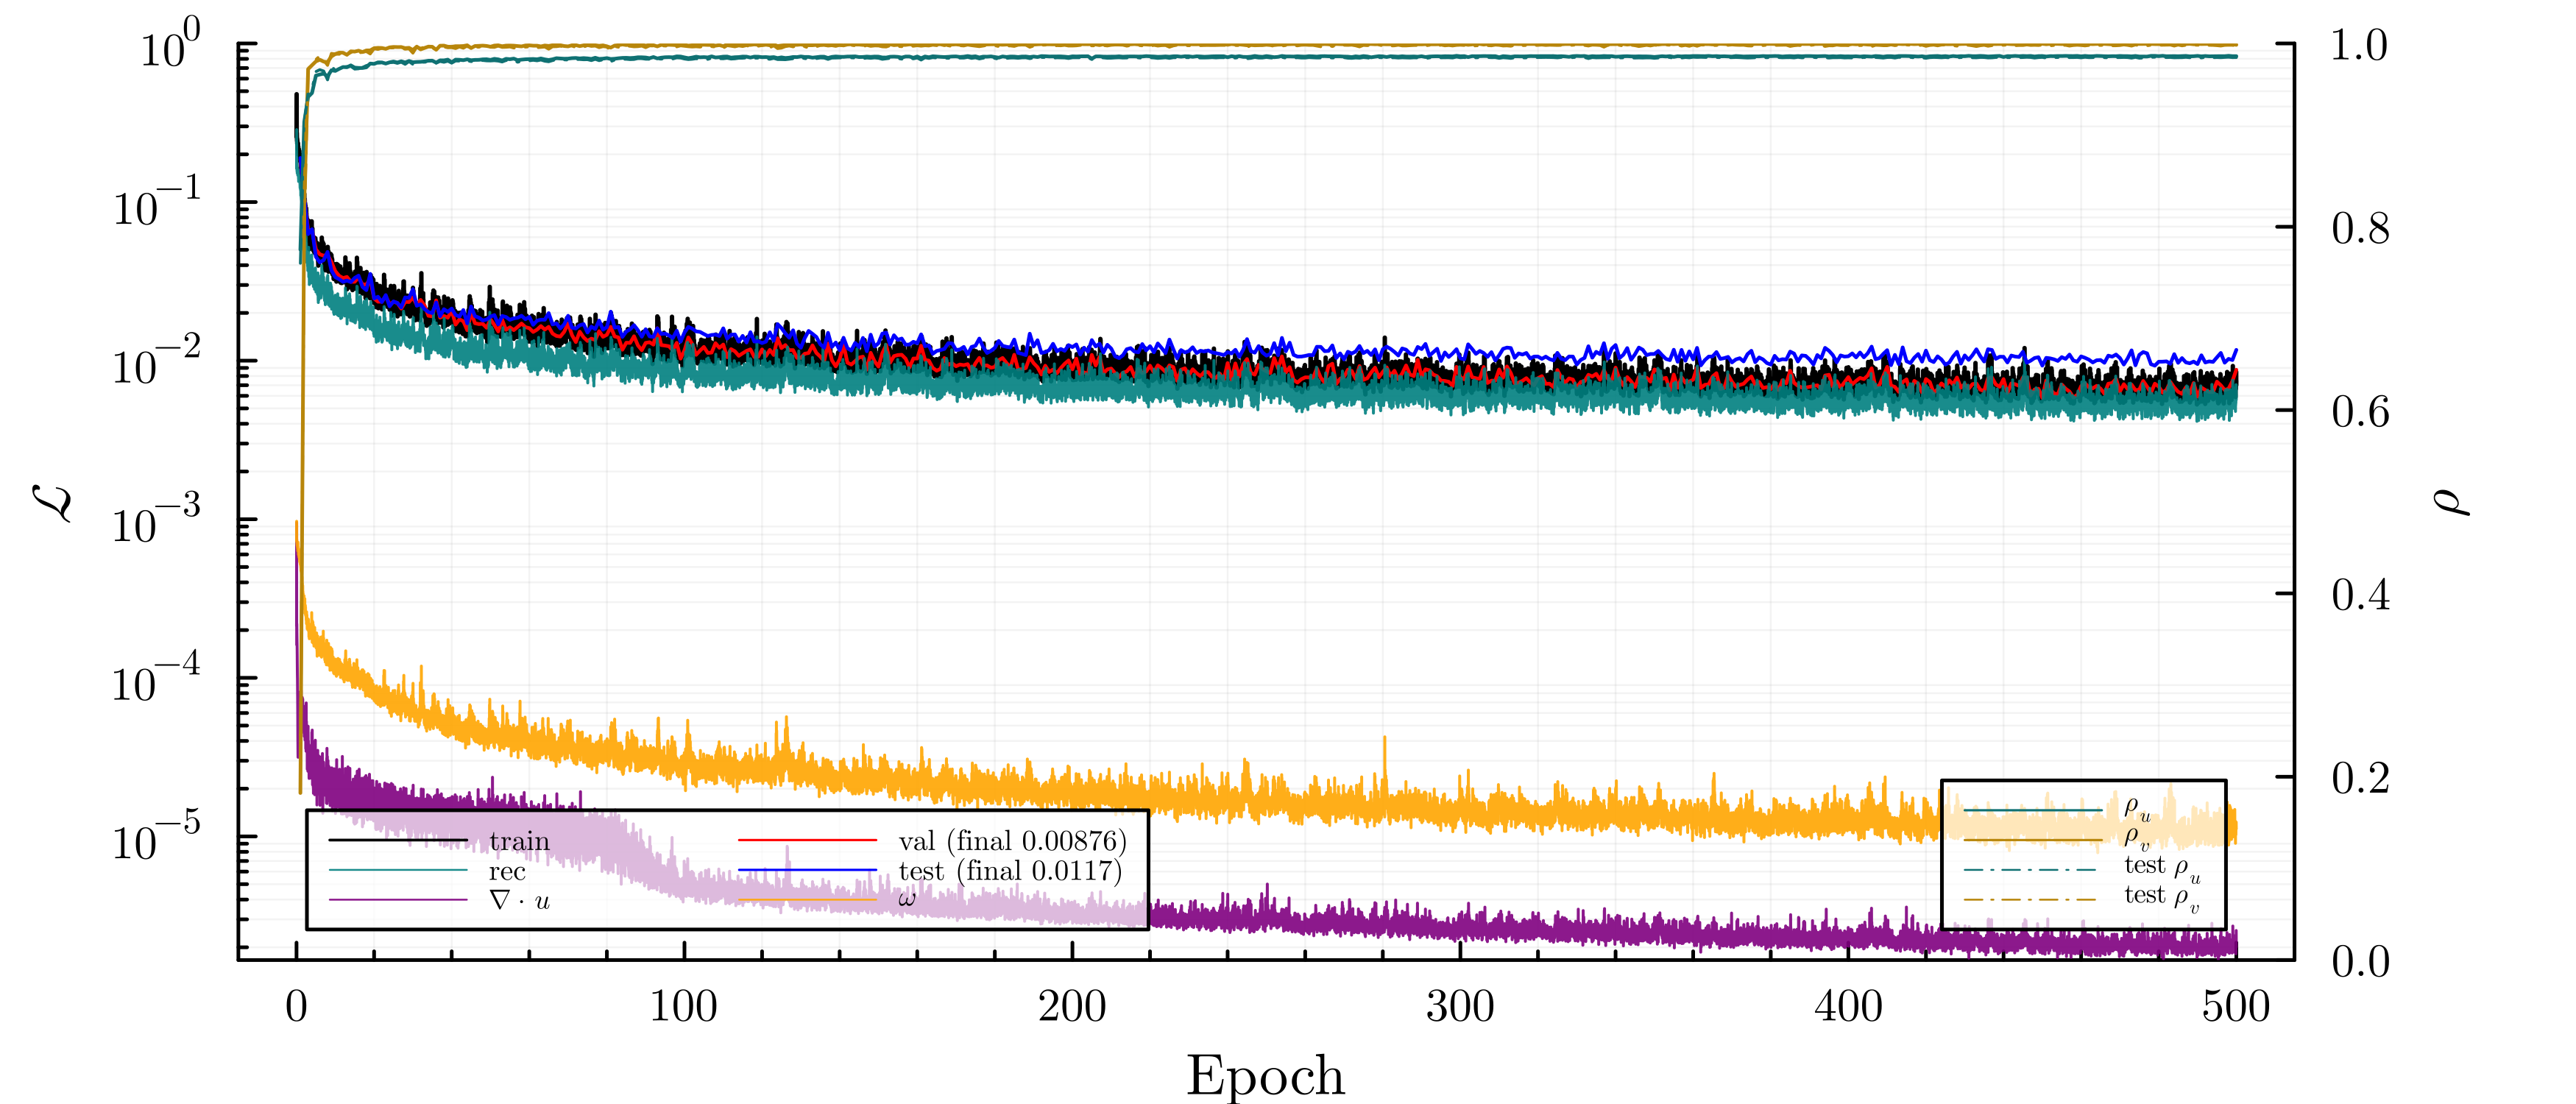
\includegraphics[width=\linewidth]{figures/Results/finer/loss_evolution.png}
    \caption{Initial training history of the autoencoder at $512^2$. Left axis ($\mathcal{L}$, logarithmic): total loss on the train, validation and test splits with the divergence ($\nabla\!\cdot\mathbf{u}$) and vorticity ($\omega$) penalties on the test split. Right axis ($CC$): reconstruction correlation coefficients $CC_u,\,CC_v$ on train and test. Validation and test losses converge to $8.6\times10^{-3}$ and $1.2\times10^{-2}$.}
    \label{fig: finer_loss}
\end{figure}

\autoref{fig: finer_loss} shows the autoencoder converging to $\mathcal{L}\approx8.6\times10^{-3}$ on the validation split and $1.2\times10^{-2}$ on the held-out test window, against $1.5\times10^{-2}$ and $3.6\times10^{-2}$ at $256^2$ (\autoref{fig: initial_training_base}).The train, validation and test curves now collapse onto one another, whereas the base case retained a test-to-validation gap of roughly a factor of two; the finer grid therefore generalises across the full simulation window rather than overfitting the initial data-gathering horizon, and $CC_u,\,CC_v$ reach unity within the first epochs.

The rapid convergence of the autoencoder shows that a large part of the training budget is spent unnecessarily: the train, validation and test losses practically collapse onto each other well before the end of the run, so there is no need to train over such a long epoch window. Since the initial autoencoder training consumes almost half of the complete integrated-workflow budget, reducing the epoch count translates directly into a higher effective speedup. If the initial autoencoder were trained for only $100$ epochs, its training cost would drop to $20\%$ of its current value. Together with a shorter update window for the retraining runs, the complete training wall time would fall to $1148.4$~s while preserving the reconstruction accuracy, since the loss is already converged at $100$ epochs. This yields an effective speedup of

\begin{align}
    S_\text{eff}
    &= \frac{T_\text{wall}^\text{ref}}{T_\text{wall}^\text{h, tot} + T_\text{wall}^\text{h, training}}
    = \frac{954.84}{401.883 + 1148.4}
    = \frac{954.84}{1550.28} \approx 0.62
\end{align}

This value shows that trimming the autoencoder schedule alone lifts $S_\text{eff}$ from $0.06$ at the base resolution to $0.62$ here, an order-of-magnitude gain that moves the integrated workflow from roughly ten times slower than the reference to within a factor of two of break-even, without touching the inference loop itself. It demonstrates that the cost of the framework is dominated by one-off training rather than by the accelerated integration: the inference loop is already cheaper than the reference, and the finer the grid, the larger that margin becomes. A single from-scratch run does not yet break even, but closing the remaining gap no longer requires a faster rollout; it requires either better use of the trained $\mathcal{P}$ across runs or overlapping training with the live simulation, together with a less strict integration monitor and switching schedule to convert the available loop speedup into actual wall-time savings.

A faithful velocity reconstruction is a key setup for the hybrid loop to accurately reproduce the loading on the cylinder. Since the force coefficients on the cylinder are calculated from the decoded velocity $\hat{\mathbf{u}}$; a reconstruction that preserves the near-body velocity, together with the divergence and vorticity penalties, feeds a more accurate pressure projection and, in turn, a more accurate integrated force. This behaviour can be seen when the force coefficients are displayed over the simulation time window in \autoref{fig: finer_forces}.

\begin{figure}[htp]
    \centering
    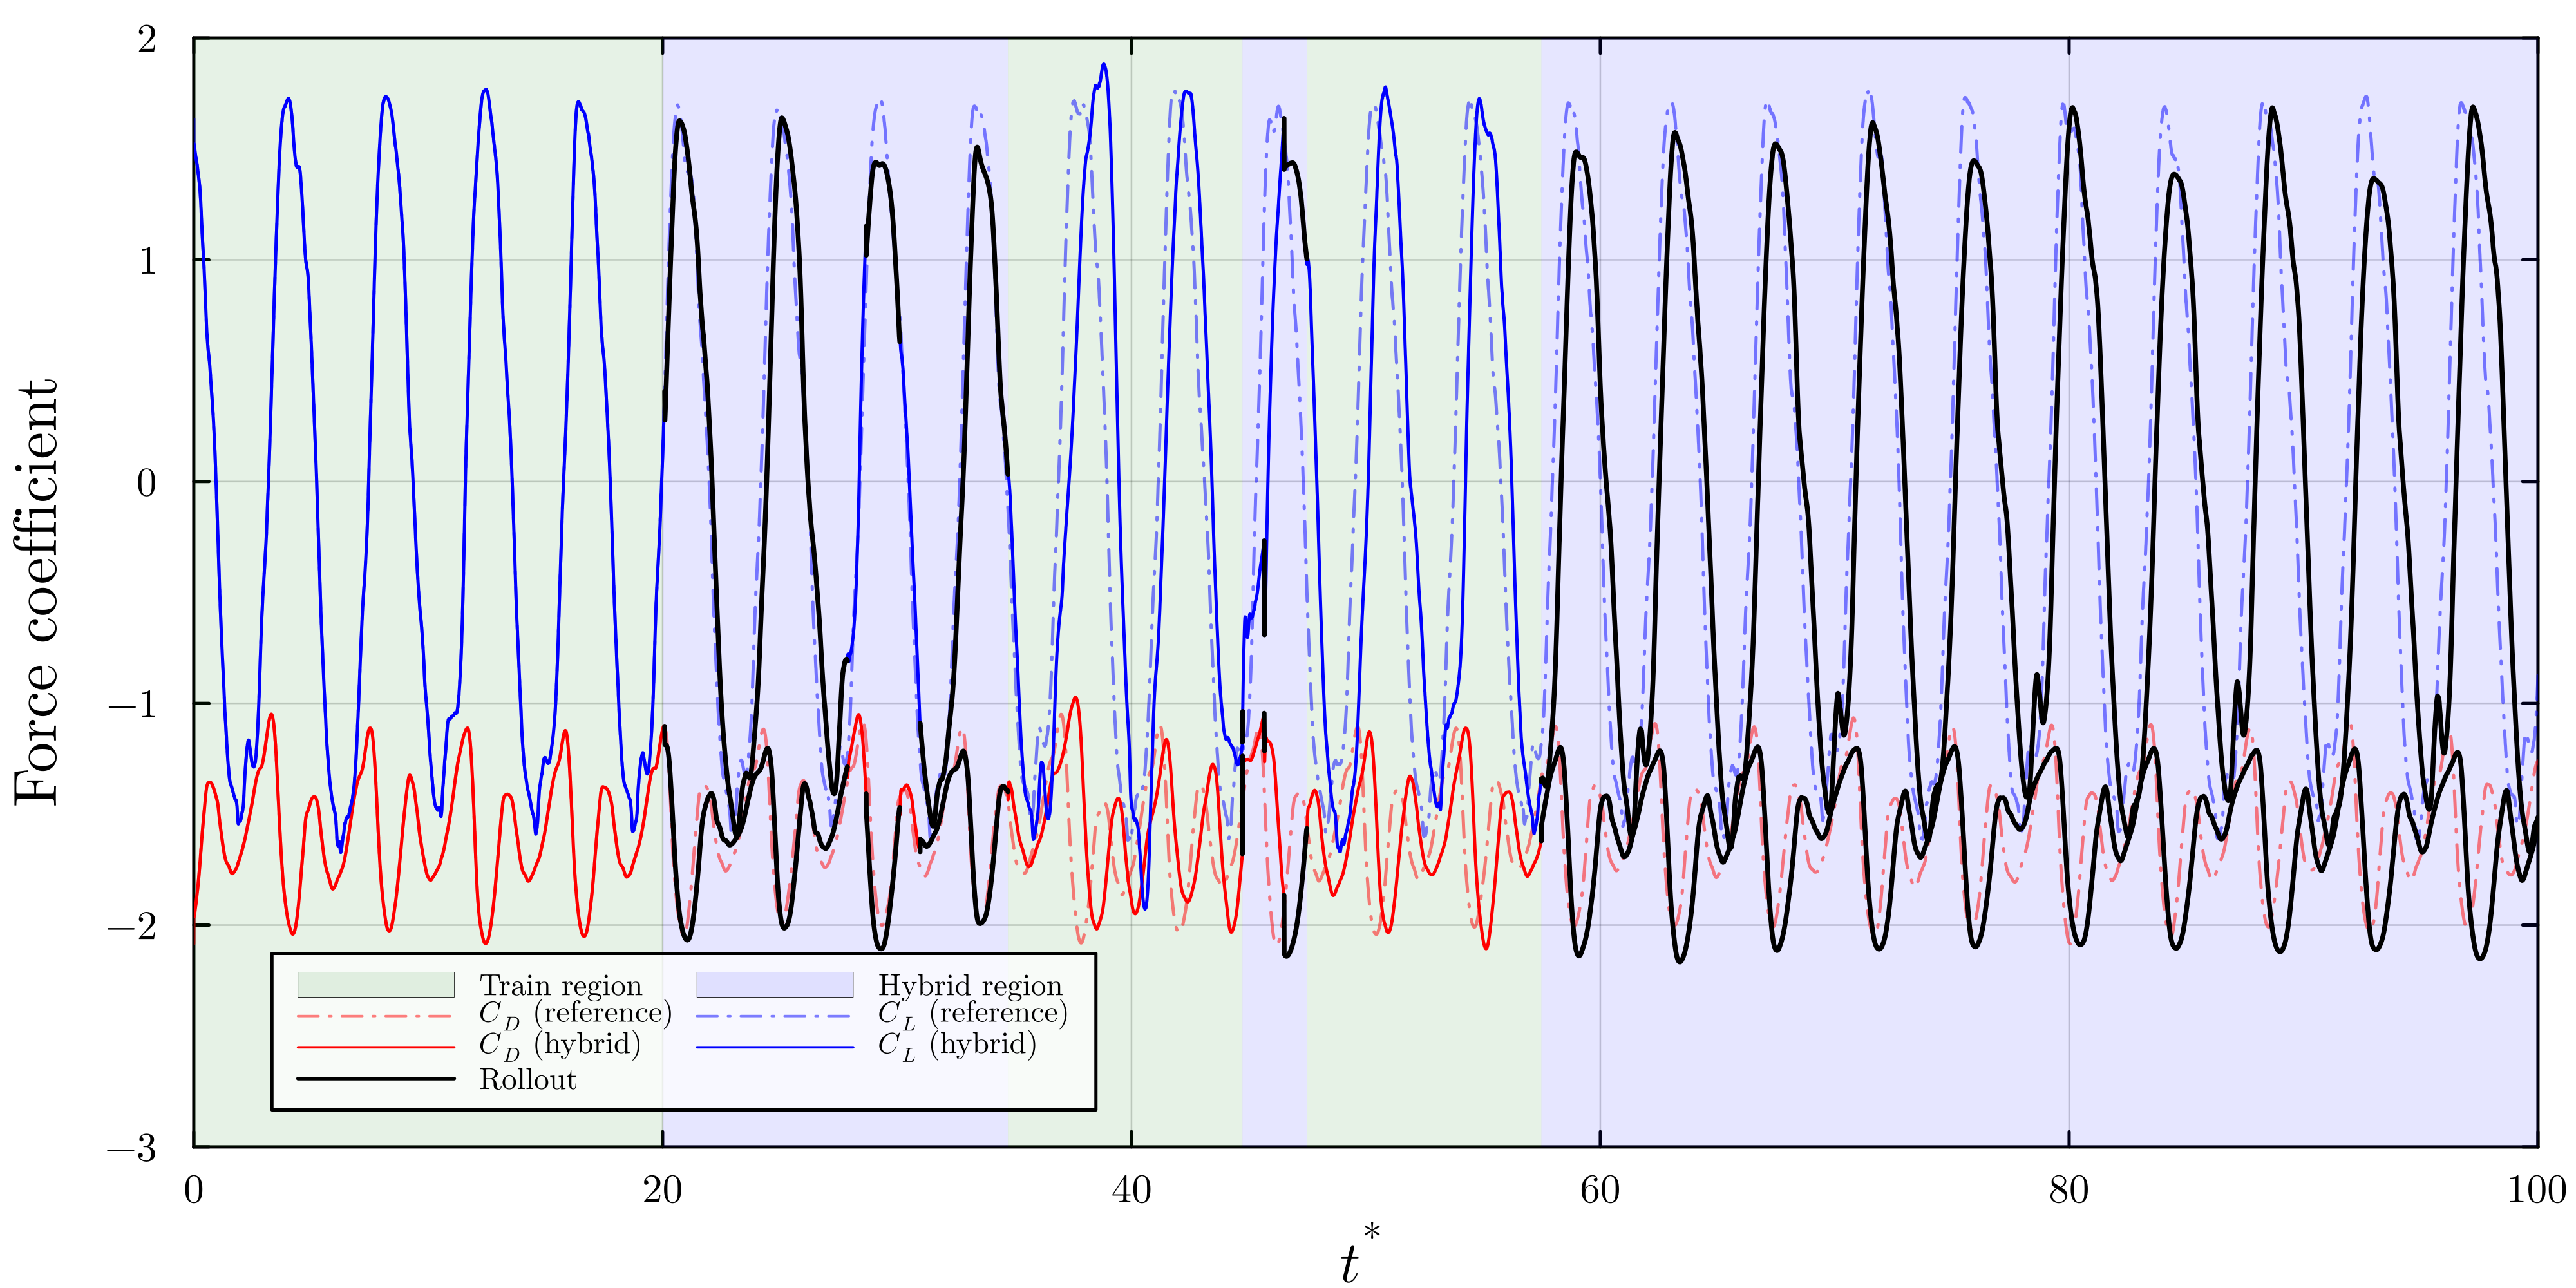
\includegraphics[width=.9\linewidth]{figures/Results/finer/forces.png}
    \caption{Lift ($C_L$) and drag ($C_D$) coefficients over $t^*$ for the finer ($512^2$) run at $Re=2500$. The hybrid loop (dashed) tracks the reference (solid) closely as an effect of the greater autoencoder performance; retraining is triggered at $t^* \approx 34.7$ and $t^* \approx 47.5$}
    \label{fig: finer_forces}
\end{figure}

\autoref{fig: finer_forces} shows that the rollouts correctly track the reference $\langle C_D \rangle$ and retain the primary shedding frequency over both the hybrid windows and the complete simulation window, with the lift preserving the shedding frequency while its fluctuation amplitude decays slightly within each rollout. This physical agreement is quantified in \autoref{tab: finer_forces}: the time-averaged drag is reproduced to within $0.64\%$ in the hybrid regions, and the time-averaged fields of \autoref{tab: finer_field} correlate with the reference at $\rho \geq 0.9966$ across the mean flow and all three Reynolds-stress
components. The only quantity that carries a visible rollout error is the lift fluctuation: the peak-weighted $C_L^\text{rms}$ error rises from $2.36\%$
over the full window to $6.83\%$ when the average is restricted to the hybrid regions. 

\begin{table}[htp]
    \centering
    \footnotesize
    \begin{subtable}[t]{0.56\textwidth}
        \centering
        \setlength{\tabcolsep}{4pt}
        \begin{tabular}{@{}lrrrr@{}}
            \toprule
            Quantity & Ref. & Hybrid & $e_\text{abs}$ & $e_\text{rel}$ [\%] \\
            \midrule
            \multicolumn{5}{l}{\textit{Full window} ($t^*\in[0,100]$)} \\
            $\langle C_D \rangle$ & $-1.57894$ & $-1.58510$ & $0.00616$ & $0.390$ \\
            $C_L^\text{rms}$      & $1.17231$  & $1.14463$  & $0.02768$ & $2.361$ \\
            \midrule
            \multicolumn{5}{l}{\textit{Hybrid regions only}} \\
            $\langle C_D \rangle$ & $-1.57201$ & $-1.58206$ & $0.01006$ & $0.640$ \\
            $C_L^\text{rms}$      & $1.16576$  & $1.08611$  & $0.07965$ & $6.832$ \\
            \bottomrule
        \end{tabular}
        \caption{Integrated force coefficients: time-mean drag
        $\langle C_D \rangle$ and r.m.s.\ lift $C_L^\text{rms}$ against the
        reference, with absolute and relative errors.}
        \label{tab: finer_forces}
    \end{subtable}
    \hfill
    \begin{subtable}[t]{0.40\textwidth}
        \centering
        \setlength{\tabcolsep}{5pt}
        \begin{tabular}{@{}lrr@{}}
            \toprule
            Quantity & $\varepsilon$ (MAE) & $\rho$ \\
            \midrule
            \multicolumn{3}{l}{\textit{Mean flow}} \\
            $\langle u \rangle$    & $0.004$ & $0.9989$ \\
            $\langle v \rangle$    & $0.004$ & $0.9970$ \\
            \midrule
            \multicolumn{3}{l}{\textit{Reynolds stresses}} \\
            $\langle u'u' \rangle$ & $0.002$ & $0.9976$ \\
            $\langle v'v' \rangle$ & $0.003$ & $0.9996$ \\
            $\langle u'v' \rangle$ & $0.001$ & $0.9966$ \\
            \bottomrule
        \end{tabular}
        \caption{Time-averaged field statistics over $\Omega$: mean absolute
        error $\varepsilon$ and spatial correlation $\rho$.}
        \label{tab: finer_field}
    \end{subtable}
    \caption{Hybrid-loop accuracy at the finer $512^2$ resolution.
    (a) integrated loading; (b) mean-flow and Reynolds-stress fields.}
    \label{tab: finer_accuracy}
\end{table}

\subsection{Latent dynamics}
\autoref{fig: finer_trajectories} shows the latent dynamics of $f_\phi$ at the finer resolution. The converged multiple-shooting fit (\autoref{fig: finer_retrain_node_ms}) reproduces all four representative components across the time windows, with $\tilde{z}$ overlaying the reference $z$ continuously through the shooting-segment boundaries of the earlier windows. The last plot of the training trajectories does show discontinuities at the segment boundaries. This mirrors the retraining imbalance identified for the base case (\autoref{subsect: 4_baseline}): since the newly augmented snapshots form a minority of the training set, so the multiple-shooting loss stays dominated by the older, well-represented dynamics and $f_\phi$ fits the newest state only weakly. 


\begin{figure}[htbp]
    \centering
    \begin{subfigure}[t]{0.48\textwidth}
        \centering
        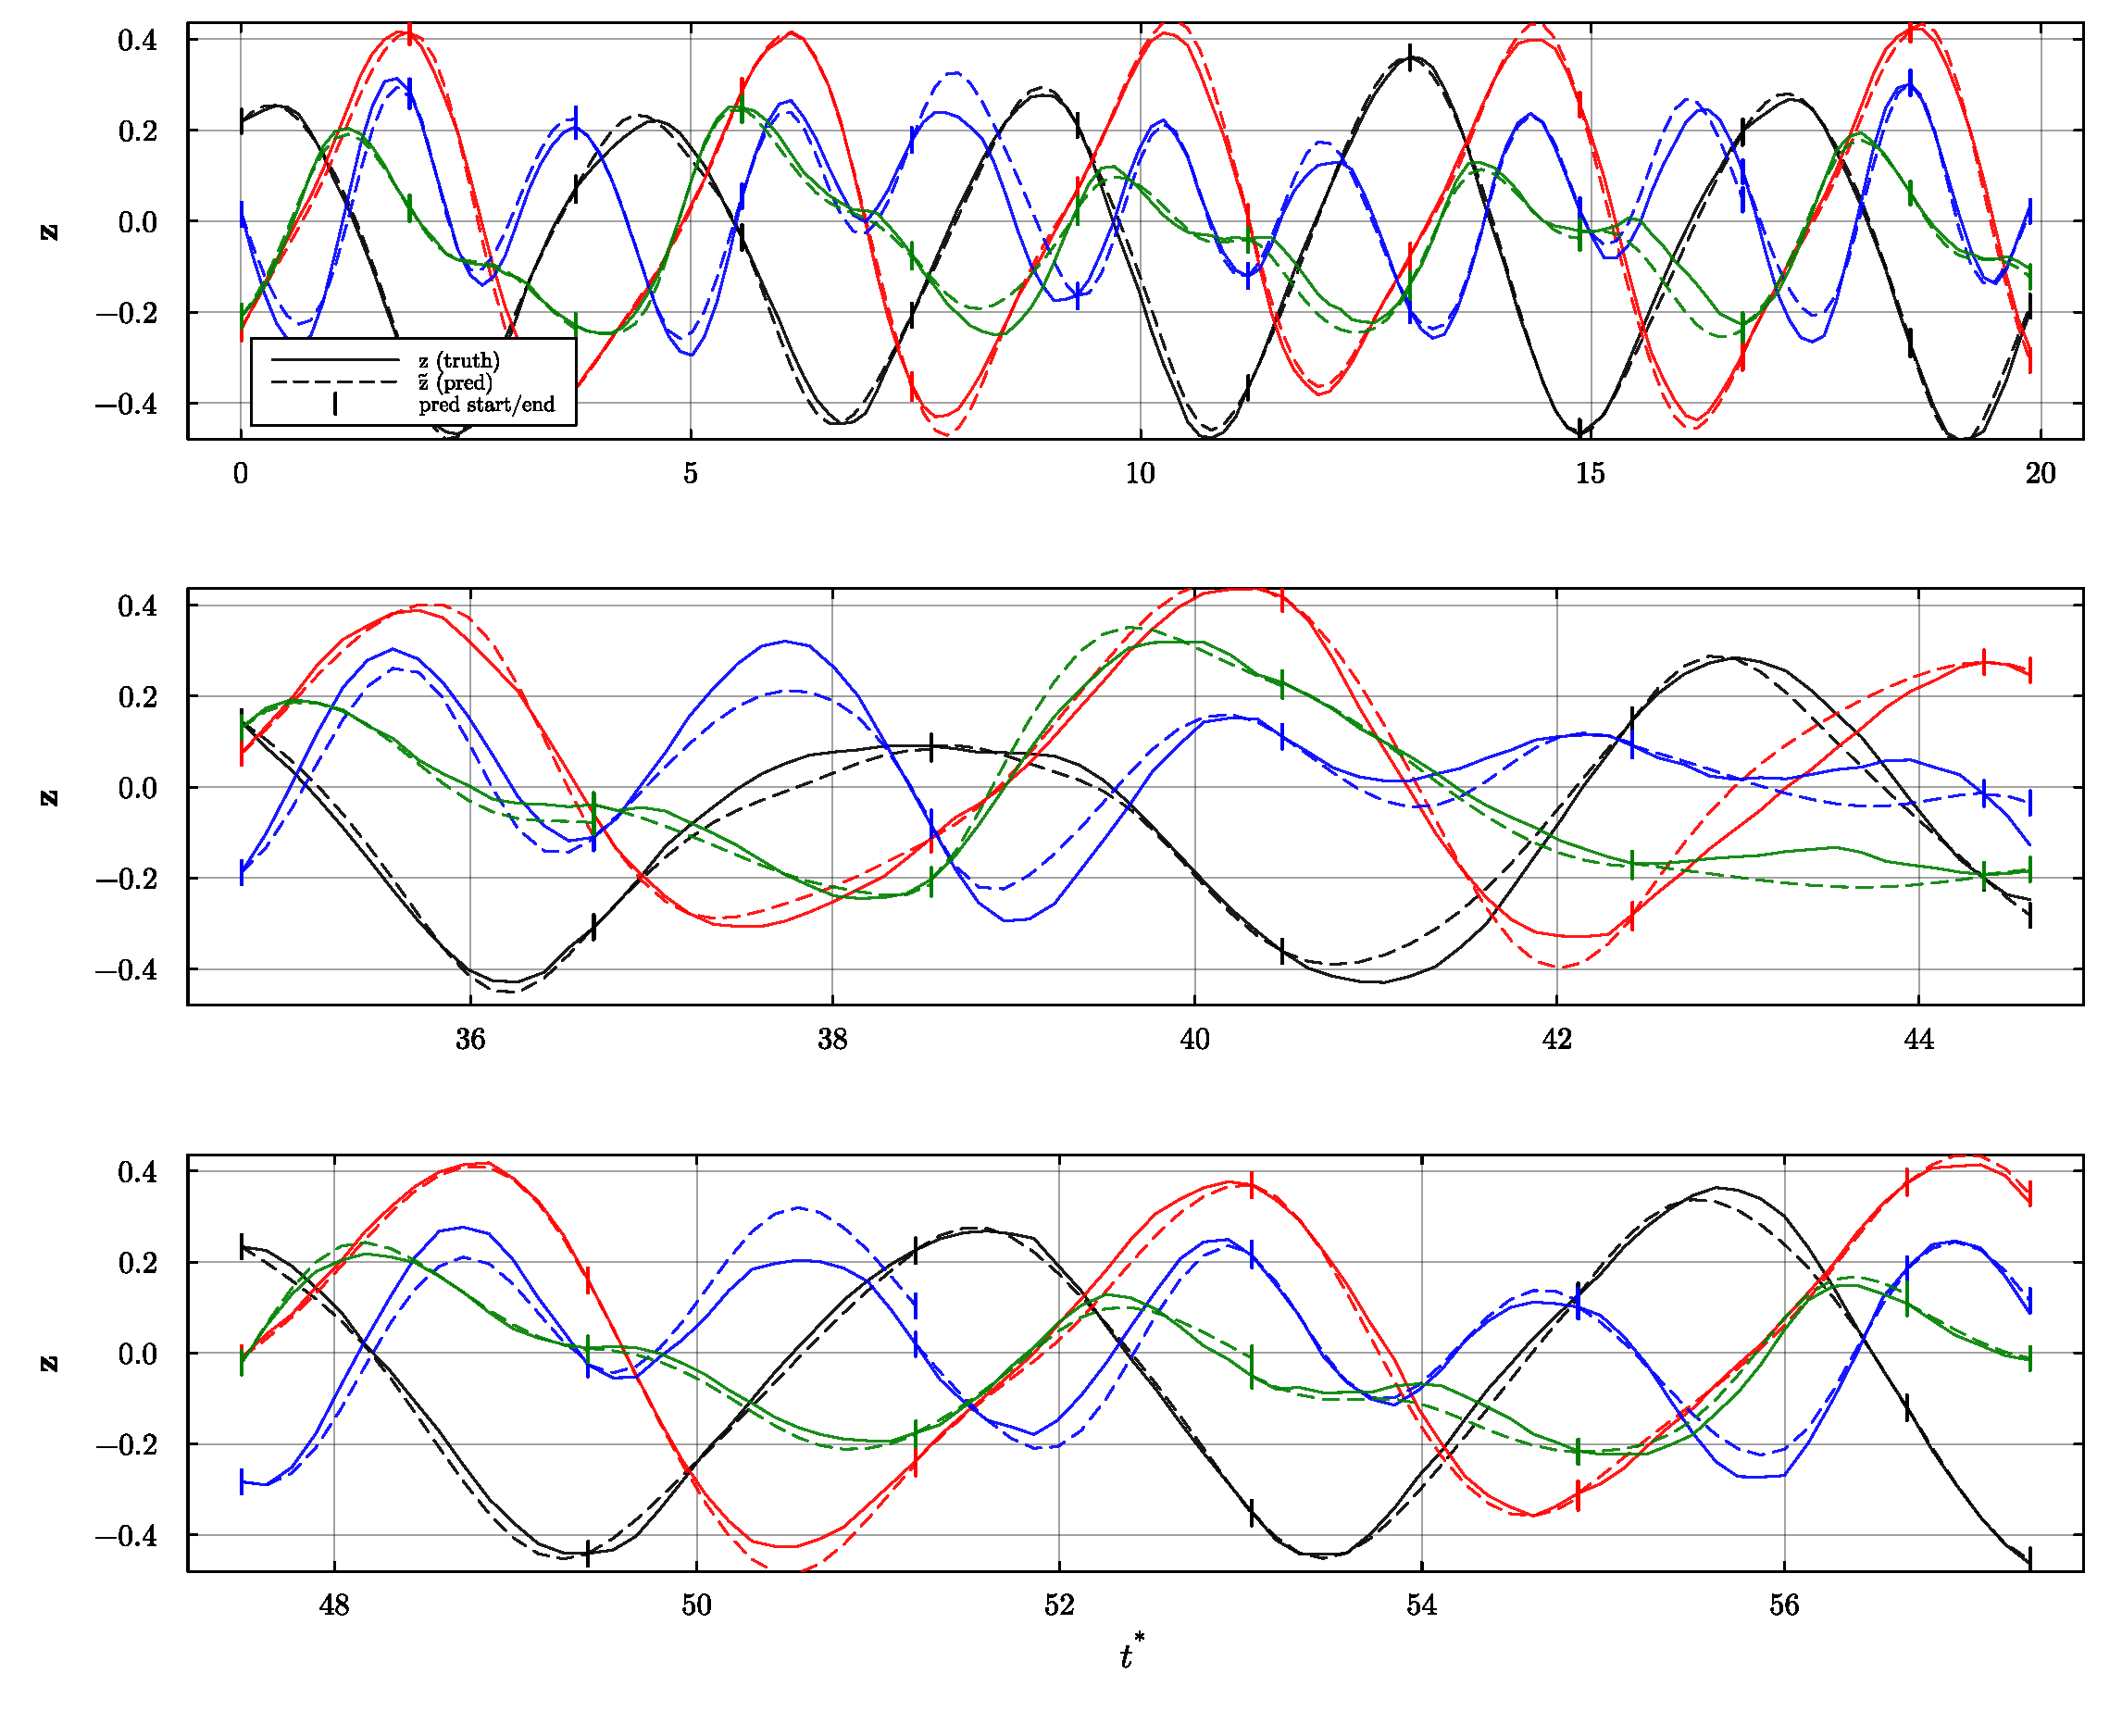
\includegraphics[width=\linewidth]{figures/Results/finer/trajectories.pdf}
    \caption{Converged multiple-shooting fit on the augmented trajectory set; markers denote shooting-segment boundaries.}
    \label{fig: finer_retrain_node_ms}
    \end{subfigure}
    \begin{subfigure}[t]{0.48\textwidth}
        \centering
        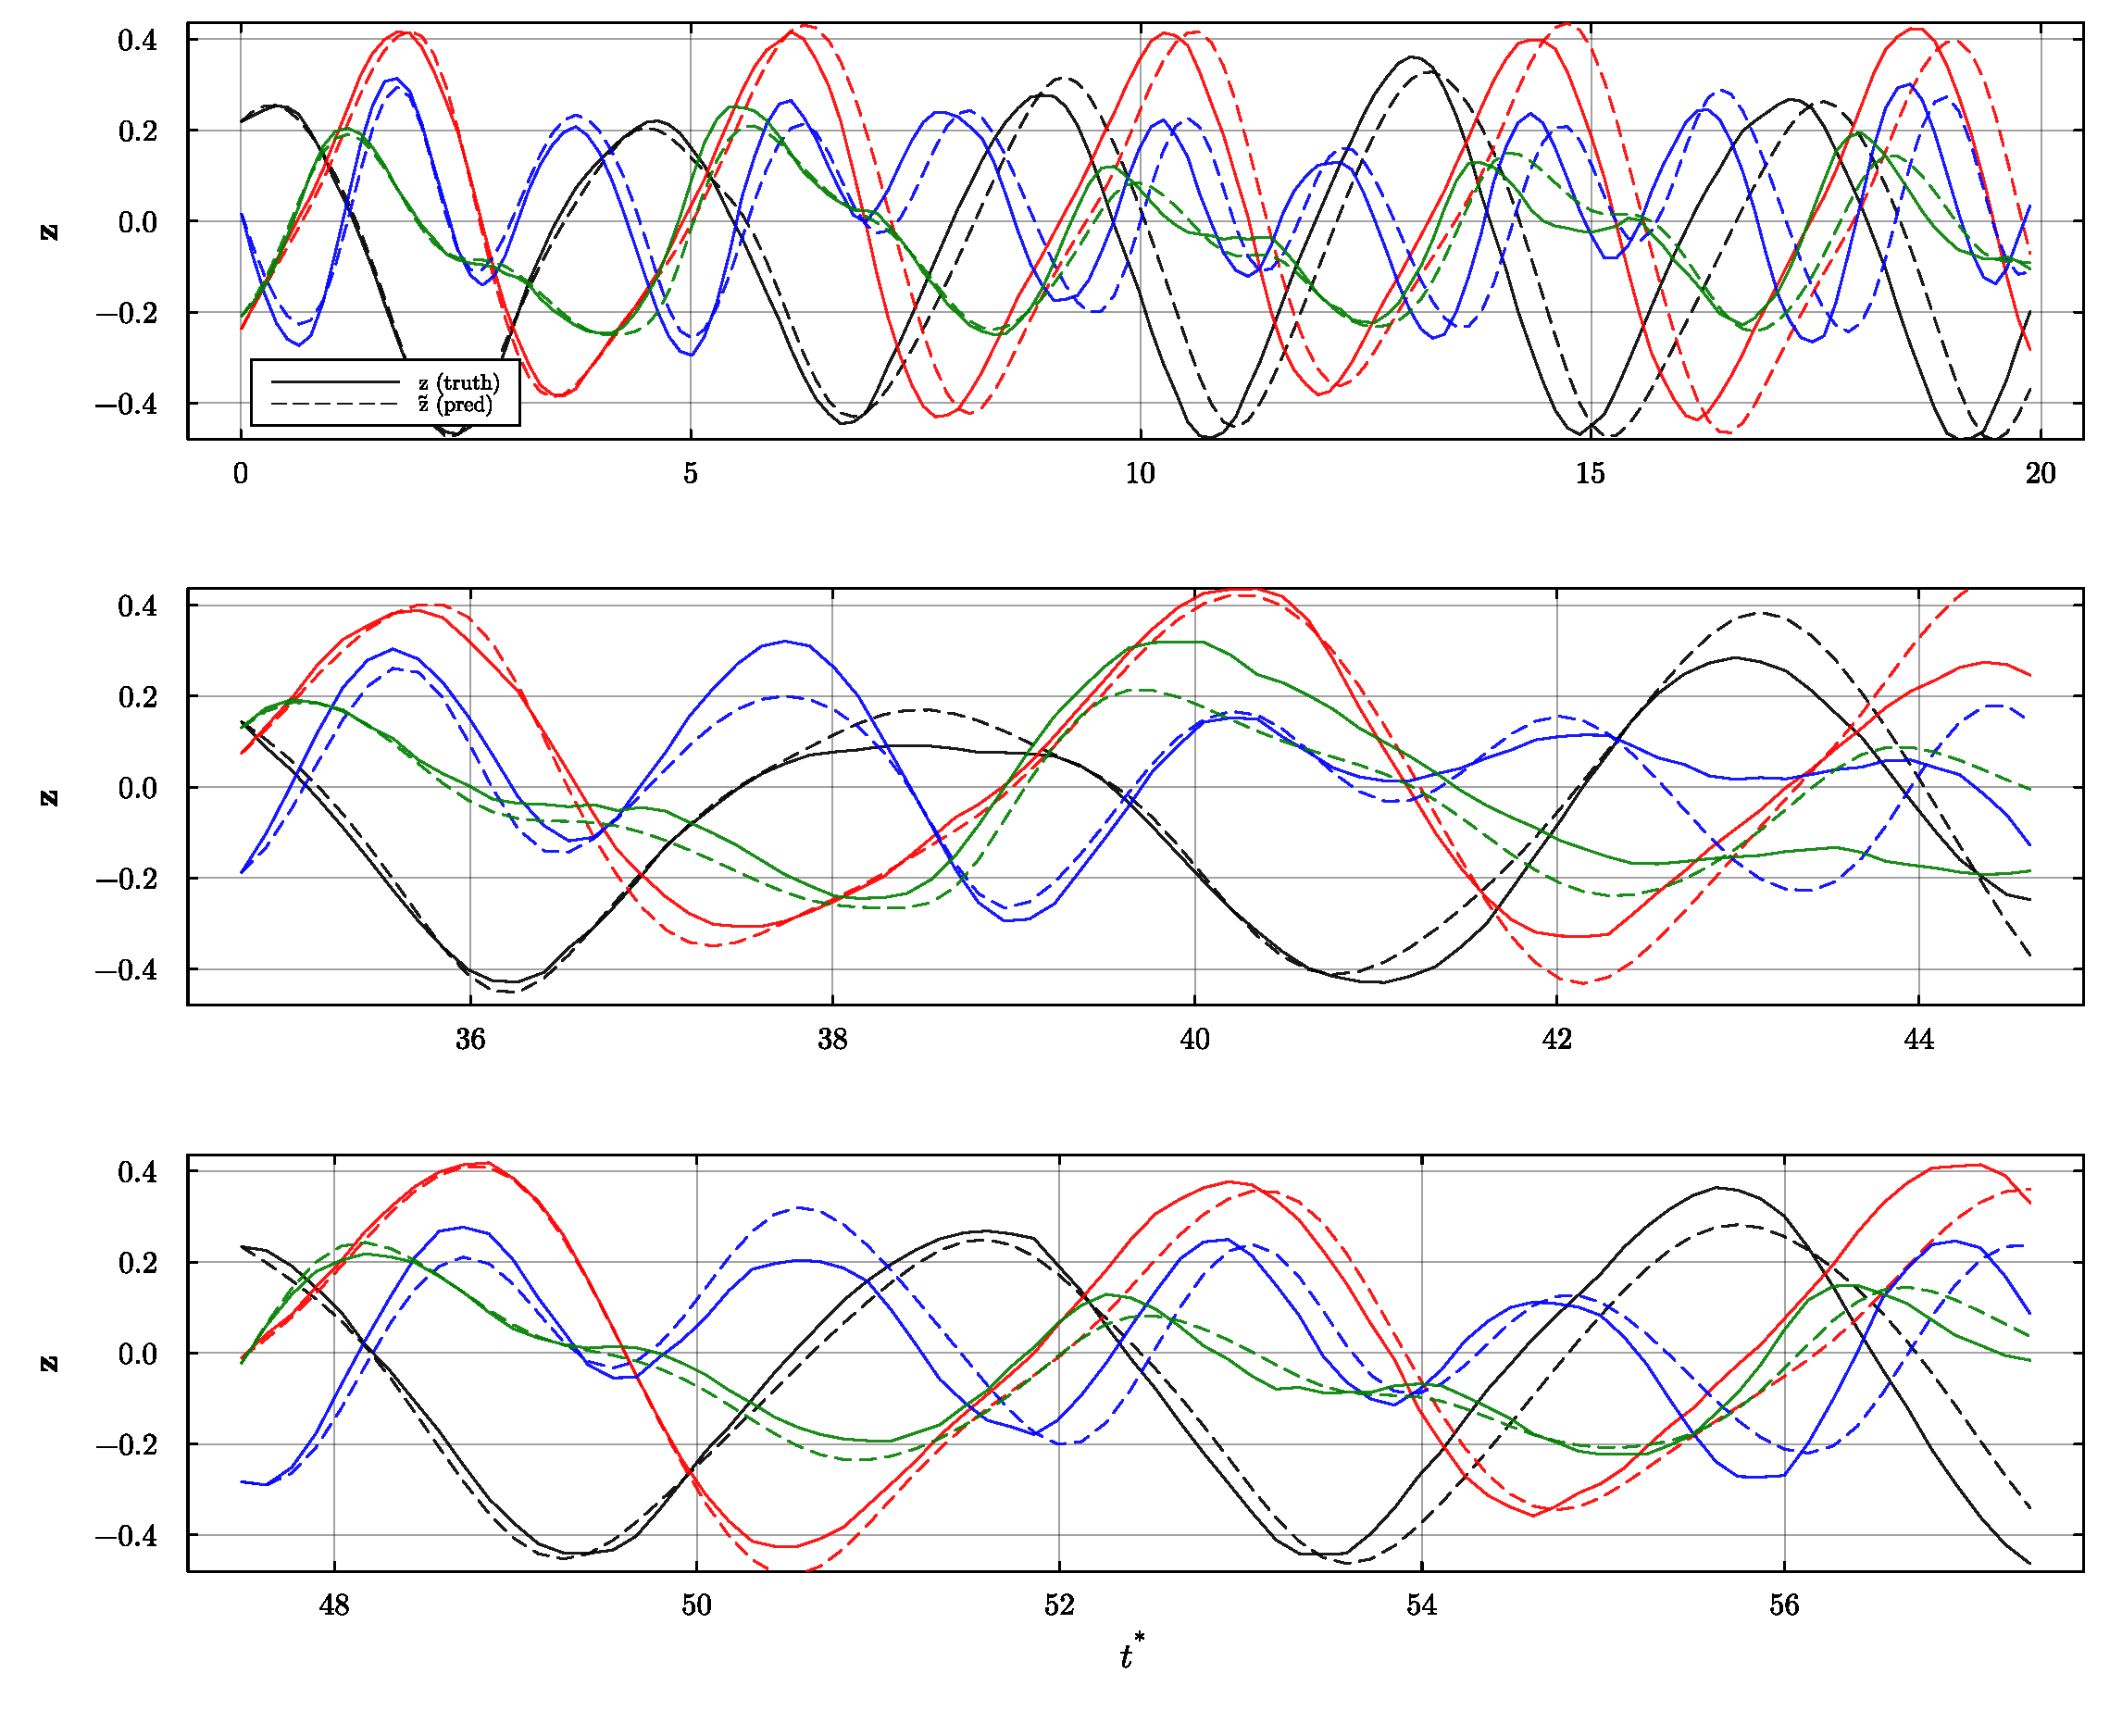
\includegraphics[width=\linewidth]{figures/Results/finer/rollout_single_shooting.pdf}
    \caption{Single rollout from $t^*=0$ across both windows after the first retraining, no segment resets.}
    \label{fig: finer_retrain_node_singleshoot}
    \end{subfigure}
    \caption{Latent dynamics of $f_\phi$ at finer grid resolution $512^2$, four representative components shown over all time windows. Reference $z$ (solid) against prediction $\tilde{z}$ (dashed). (a) Converged multiple-shooting fit on the augmented trajectory set, with segment start/end markers; (b) unaided single rollout from $t^*=0$ over the same windows.}
    \label{fig: finer_trajectories}
\end{figure}

The latent components produced by the highly accurate $\varphi_\theta$ are smooth and low in amplitude variance, showing a compact, near-periodic orbit in latent space rather than a broadly scattered cloud. Parallel to the low Re hybrid simulation discussed in \autoref{subsect: 4_re250}, this compact spread of latent vectors tightens the KNN monitor threshold $\tau$. Since the tightly clustered latent space yields small in-distribution scores and hence a small absolute $\tau$. Any divergent predictions of $\tilde{z}$ get flagged as OOD quickly and control is handed back to WaterLily, which is what caps the rollout length and forces the speedup at this resolution to come from the training budget (\autoref{subsect: 4_finer_walltime}) rather than from longer rollouts. 

The finer $512^2$ grid shows that the hybrid framework is transferable to a higher resolution without modification: the autoencoder reconstructs the velocity field more accurately and converges in a fraction of the epoch budget, the integrated drag and time-averaged fields remain near to the reference simulation, and the larger reference cost combined with the trimmable training schedule lifts the projected effective speedup by an order of magnitude over the base case. These results are promising but not complete. The $S_\text{eff}$ estimate rests on a single measured run and on the assumption that the turbulent statistics remain converged at the reduced epoch count, and the rollout length is still capped by the tight integration monitor. A dedicated study at finer resolution, covering the epoch--statistics trade-off, a measured rather than projected wall-time breakdown, and a less conservative gating schedule, could prove to be an interesting way to determine the true performance of this framework. 

